% !TEX TS-program = pdflatex
% !TEX encoding = UTF-8 Unicode

% This is a simple template for a LaTeX document using the "article" class.
% See "book", "report", "letter" for other types of document.

\documentclass[11pt]{article} % use larger type; default would be 10pt

\usepackage[utf8]{inputenc} % set input encoding (not needed with XeLaTeX)

%%% Examples of Article customizations
% These packages are optional, depending whether you want the features they provide.
% See the LaTeX Companion or other references for full information.

%%% PAGE DIMENSIONS
\usepackage{geometry} % to change the page dimensions
\geometry{a4paper} % or letterpaper (US) or a5paper or....
% \geometry{margin=2in} % for example, change the margins to 2 inches all round
% \geometry{landscape} % set up the page for landscape
%   read geometry.pdf for detailed page layout information

\usepackage{graphicx} % support the \includegraphics command and options

% \usepackage[parfill]{parskip} % Activate to begin paragraphs with an empty line rather than an indent

%%% PACKAGES
\usepackage{booktabs} % for much better looking tables
\usepackage{array} % for better arrays (eg matrices) in maths
\usepackage{paralist} % very flexible & customisable lists (eg. enumerate/itemize, etc.)
\usepackage{verbatim} % adds environment for commenting out blocks of text & for better verbatim
\usepackage{subfig} % make it possible to include more than one captioned figure/table in a single float
% These packages are all incorporated in the memoir class to one degree or another...

%%% HEADERS & FOOTERS
\usepackage{fancyhdr} % This should be set AFTER setting up the page geometry
\pagestyle{fancy} % options: empty , plain , fancy
\renewcommand{\headrulewidth}{0pt} % customise the layout...
\lhead{}\chead{}\rhead{}
\lfoot{}\cfoot{\thepage}\rfoot{}

%%% SECTION TITLE APPEARANCE
\usepackage{sectsty}
\allsectionsfont{\sffamily\mdseries\upshape} % (See the fntguide.pdf for font help)
% (This matches ConTeXt defaults)

%%% ToC (table of contents) APPEARANCE
\usepackage[nottoc,notlof,notlot]{tocbibind} % Put the bibliography in the ToC
\usepackage[titles,subfigure]{tocloft} % Alter the style of the Table of Contents
\renewcommand{\cftsecfont}{\rmfamily\mdseries\upshape}
\renewcommand{\cftsecpagefont}{\rmfamily\mdseries\upshape} % No bold!

%%% END Article customizations

%%% The "real" document content comes below...

\title{\huge{Bennington College Small Radio Telescope} \\ Operations Manual}
\author{}
\date{} % Activate to display a given date or no date (if empty),
         % otherwise the current date is printed 

\begin{document}
\maketitle


\vspace{4cm}

\begin{center}
\emph{\Large{Andrew Cencini – Hugh Crowl} \\ 
\large{William Buchanan, Alexander Curth, Erick Daniszewski, Evan Gall,
Clemente Gilbert-Espada, Chernoh Jalloh, Brendon Walter}}
\end{center}


\vspace{7cm}

\begin{center}
\emph{with guidance from} \\ 
\Large{\textbf{MIT Haystack Observatory's}} \\ 
Haystack Small Radio Telescope Project
\end{center}
\normalsize

\tableofcontents

\newpage

\section{Introduction}

This manual serves as a guide following the work done at Bennington College during the spring of 2014 to build and operate a radiotelescope, following the procedure layed out by MIT Haystack and their Small Radio Telescope (SRT) project. This manual contains information regarding both the hardware and software components of the project which should allow for a simple and successful build and operation of a SRT.

\section{Parts List}


\subsection{LNA to Dongle Interface}

\begin{tabular}{| p{6cm} | c | p{5cm} | l | c |}
\hline
\textbf{Part} & \textbf{Qty.} & \textbf{Manufacturer} & \textbf{Cost} \\ \hline \hline
SMA-M Crimp Connector Straight & 1 & Amphenol/Connex & \$5.95 \\ \hline
LMR-400 & 100ft & & \$102.99\\ \hline
Type-F Male Crimp Connector & 1 & Amphenol/Connex &\$4.95 \\ \hline
In-Line Amplifier & 1 & Blonder Tongue & \$8.22 \\ \hline
BNC Female Jack to Type-F Male Plug & 3 & & \$10.99 \\ \hline
BNC-M to BNC-M Patch Cable & 3 & Amphenol RF & \$12.55 \\ \hline
Power Injector & 1 & Channel Vision & \$14.71 \\ \hline
BNC-F to SMA-M Adapter & 1 & Vitelec / Emerson Connectivity Solutions & \$12.09 \\ \hline
Bandpass Filter & 1 & Mini-Circuits & \\ \hline
SMA-F to BNC-F Adapter & 1 & AIM-Cambridge / Emerson Connectivity Solutions & \$4.21 \\ \hline
BNC-F to SMB Plug Adapter & 1 & & \$8.49 \\ \hline
AC-to-DC Power Supply & 1 & & \$20.18 \\ \hline
Breadboard & 1 & Vector Electronics & \$5.75 \\ \hline
DC Jack & 1 & CUI Inc & \$1.00 \\ \hline
F-Type Plug & 1 & Bomar Interconnect/ Winchester Electronics & \$4.16\\ \hline
\end{tabular}

\subsection{Feed}

\begin{tabular}{| p{6cm} | c | p{5cm} | l | c |}
\hline
\textbf{Part} & \textbf{Qty.} & \textbf{Manufacturer} & \textbf{Cost} \\ \hline \hline
Ultra Low Noise Amplifier & 1 & Mini-Circuits & \\ \hline
Coaxial Bias-Tee & 1 & Mini-Circuits & \\ \hline
Coaxial Cable 086-6SM+ & 1 & Mini-Circuits & \\ \hline
Coaxial Cable 086-4SM+ & 1 & Mini-Circuits & \\ \hline
SMA-F to SMA-F Adapter & 1 & Mini-Circuits & \\ \hline
SMA-F to Solder Pin Bulkhead Connector & 1 & Emerson Network Power Connectivity Johnson & \$8.06 \\ \hline
SMA-M to SMA-M Right Angle Adapter & 1 & & \\ \hline
3M Adhesive Copper Foil Tape & 1 & 3M & \\ \hline
22 Gauge Copper Wire & 1 & & \\ \hline
Semi-Rigid Coaxial Cable & 1 & Micro-Coax & \$4.62 \\ \hline
F-Type Male to BNC Female & 1 & & \$0.89 \\ \hline
SMA-M to SMA-M Coupler & 1 & & \$7.49\\ \hline
\end{tabular}



\section{Tools List}

\subsection{Assembling the LNA and Feed}

\begin{tabular}{| l | p{10cm} |}
\hline
\textbf{Tool} & \textbf{Description} \\ \hline \hline
Soldering iron + solder & soldering components as specified by Haystack documentation \\ \hline
Wire cutter/ strippers & cutting 22 gauge copper wire\\ \hline
Screwdriver & assembling box of LNA\\ \hline
Labeler & labeling LNA\\ \hline
Hacksaw & cutting styrofoam\\ \hline
Metric measuring tape & measuring styrofoam, and helix position\\ \hline
Drill press and 1/4" bit & drilling hole into styrofoam, LNA baseplate, cake pan, pc board\\ \hline
X-acto knife & cutting copper tape\\ \hline
Straight edge & cutting copper tape\\ \hline
Marker & marking position of helix\\ \hline
\end{tabular}


\subsection{Assembling the Dish}

\begin{tabular}{| l | p{10cm} |}
\hline
\textbf{Tool} & \textbf{Description} \\ \hline \hline
Socket wrench set & bolting arms onto center\\ \hline
Hammer and tap & marking ends of arms and outer band to make drilling holes easier\\ \hline
Handheld Riveter/ rivets & riveting the outer band and strips over mesh on the arms.\\ \hline
Hacksaw & \\ \hline
Power drill + Drill bit & drilling holes to place rivets connecting outerband, mesh, strips, and dish arms\\ \hline
Safety Gloves & for your fingers\\ \hline
Pliers & Useful for bending mesh when wrapping around edge\\ \hline
Tin Snips & cutting mesh\\ \hline
Pen/Marker & mark hole locations pre-drilling\\ \hline
\end{tabular}


\subsection{Building the Mount}

\subsection{Attaching Arms}

\subsection{Mounting Dish}




\section{Installing SRTN Software}

The original SRT source can be found on the MIT Haystack Observatory website, here: http://www.haystack.mit.edu/edu/undergrad/srt/ . This source appears to work with ArchLinux and CentOS, and reportedly works on REHL (Red Hat Enterprise Linux). The source will not work immediately with Ubuntu, however a modified version of the source can be found here: https://github.com/BenningtonCS/Telescope-2014 , which will work on Ubuntu, as well as CentOS and ArchLinux (It may work with other linux-based operating systems, however, those listed are the only ones we have tested so far). 

\subsection{MIT Haystack Observatory SRT}
The MIT Haystack Observatory SRT website includes the manuals, documentation, and program code. The code base we are looking at, SRT Source Code ver 3, can be found here.

\subsection{Ubuntu}


These instructions were developed as a guide from a clean download of source files from the MIT Haystack Observatory website. If using the code pulled from the repository, some of the steps (modifying the srtnmake script for example) may not be necessary, but the guide should still hold, overall.
\\ \\
Note that these instructions were written for Ubuntu 12.10

\begin{verbatim}
$ lsb_release -a
No LSB modules are available.
Distributor ID: Ubuntu
Description:    Ubuntu 12.10
Release:    12.10
Codename:   quantal
\end{verbatim}



\subsubsection{Getting the Source Code}
To get the source code, either go to the website, linked above, and download SRT Source Code ver 3, or download directly from the link above. Once downloaded, the gzipped tarball should be in your Downloads directory: 
\begin{verbatim}
~/Downloads/newsrtsource_ver3.tar.gz
\end{verbatim}

\noindent\emph{Move and Unzip File in New Directory} 
\\ \\
To create a new directory, move the gzipped tarball into it, and then unzip it, follow the commands below:
\begin{verbatim}
~$ mkdir radio
~$ mv Downloads/newsrtsource_ver3.tar.gz radio
~$ cd radio
~/radio$ tar -xzvf newsrtsource_ver3.tar.gz
~/radio$ cd srtnver3
\end{verbatim}


\subsubsection{Adding Library Dependencies}
The reason the code would not compile is because SRT uses libraries which the computer you are using does not have. To get them, use the command below:

\begin{verbatim}
~/radio/srtnver3$ sudo apt-get install libgtk2.0-dev libusb-1.0-0-dev
\end{verbatim}


NOTE: If you are unable to download using apt-get install, try using the command apt-get update first, wait for all updates to be installed, and then retry the install command above.

Modifying the Compile Script
In order for the program to compile with gtk+-2.0, it must know that it has to use it/where to get it. (This was the problem that prevented it from compiling in class). To remedy this, simply
~/radio/srtnver3\$ sudo nano srtnmake
to edit the bash script. Scroll to the bottom of the file to the gcc line, which should look like:
gcc -W -Wall -03 \$CFLAGS \$LIBS main.c vspectra\_four.c disp.c plot.c cat.c geom.c time.c outfile.c sport.c map.c cmdfl.c cal.c srthelp.c velspec.c four.c librtlsdr.c tuner\_r820t.c -lm `pkg-config --libs --cflags libusb-1.0`
and change it so the end section is now
... `pkg-config --libs --cflags gtk+-2.0 libusb-1.0`
Now you have all the libraries and the script should be able to compile successfully.

\subsubsection{Compiling the Source Code}
The script to compile the code (the one you just edited) should take care of all the compilation, so it is just a matter of running it
~/radio/srtnver3\$ ./srtnmake
Once you execute this command, a few warnings should appear, with lines ending with [-Wunused-but-set-variable]. These errors are fine, and there should be relatively few of them as compared to before (running the compile script without the libraries or modification to the script). The output I got from running the compile script is shown below as a reference for which errors are acceptable.

Now the source code is successfully compiled!

\subsubsection{Running the Program}
If you look in the srtnver3 directory, you will notice an executable file called srtn. This is what we just compiled with srtnmake. To run:
~/radio/srtnver3\$ ./srtn
Once executed, this should open a window which looks similar to the image below.


\subsection{CentOS}


These instructions were made using CentOS release 6.5 with kernel version:

\begin{verbatim}
$ uname -r
2.6.32-431.el6.x86_64
\end{verbatim}
on a machine with an AMD processor.

\subsubsection{MIT Haystack Observatory SRT}
The MIT Haystack Observatory SRT website includes the manuals, documentation, and program code. The code base we are looking at, SRT Source Code ver 3, can be found here.

\subsubsection{Getting the Source Code}
From the website, linked above, or the download link provided, download the srtnver3 source files from the MIT Haystack website. Once the download is complete, the gzipped tarball should be in your Downloads directory.

\begin{verbatim}
$ cd Downloads
$ tar xzvf newsrtsource_ver4.tar.gz
If you want to move the source code out of the Downloads directory, and into the Home directory, for example:
$ mv srtnver3 ~
$ cd ~
\end{verbatim}

\subsubsection{Getting project dependencies}
From a clean install of CentOS, you will be missing some of the packages needed to run the software.
\\ \\
\emph{Getting sudo permissions} \\ \\
Before you do this though, you need to add your profile to the sudoers file, if you do not already have sudo permissions. To do this:

\begin{verbatim}
$ su
$ chmod +w /etc/sudoers
$ gedit /etc/sudoers
\end{verbatim}

Down by the bottom of the file will be the line:

\begin{verbatim}
\#\# Allow root to run any commands anywhere
root    ALL=(ALL)    ALL
\end{verbatim}

Below this add the line " ALL=(ALL) ALL", where is the username logged in to the computer, in our case 'radio telescope'

\begin{verbatim}
\#\# Allow root to run any commands anywhere
root    ALL=(ALL)    ALL
radiotelescope    ALL=(ALL)    ALL
\end{verbatim}

Save the file and exit gedit, then in the terminal, type exit to return to your user status:

\begin{verbatim}
[root@localhost radiotelescope]\# exit
exit
[radiotelescope@localhost ~]\$
\end{verbatim}

Now your user account should have sudo permission, so we can now install package dependencies.
\\ \\
\emph{Getting dependencies}
\\ \\
The packages needed are gtk+2, gcc, and libusb. These can be acquired using the CentOS package manager, yum:

\begin{verbatim}
\$ sudo yum install gtk2-devel gcc libusb1-devel
\end{verbatim}

If successful, you should now have all the packages you need to run the software.

\subsubsection{Compiling and running}

Now, move into the srtnver3 directory
\$ cd ~/srtnver3
and run srtnmake:
\$ ./srtnmake
This should complete successfully, but may show some warning messages. Now, to run the software:
\$ ./srtn

\subsubsection{Running with unsimulated dongle}
To run with the dongle, receiver simulation must be turned off. To do this, simply
\$ gedit srt.cat
In the edit window, find the line that says
SIMULATE RECEIVER
and change it to
*SIMULATE RECEIVER
Save the file and exit gedit. Now, we can run srtn using the dongle with
\$ sudo ./srtn
And it should work!
NOTE: Notice how before to run, it was just ./srtn and this time it is sudo ./srtn. If you try./srtn after enabling the dongle you will get a message similar to:
\$ ./srtn
Found 1 device(s)
  0:  ,   SN:  ?????
Using device 0: ezcap USB 2.0 DVB-T/DAB/FM dongle
usb\_open error -3
Please fix the device permissions, e.g. by installing the udev rules file rtl-sdr.rules
Failed to open rtlsdr device \#0.
As we see above, it is possible to run srtn without sudo, but to do so, we must do a little extra work in installing the provided udev rules. A guide to installing the udev rules will be added later.

\subsubsection{Running with unsimulated controller/rotator}
To run with the controller/rotator, antenna simulation must be turned off. To do this, simply
\$ gedit srt.cat
In the edit window, find the line that says
SIMULATE ANTENNA
and change it to
*SIMULATE ANTENNA
Save the file and exit gedit. Now, we can run srtn using the controller/rotator with
\$ sudo ./srtn
To test that the rotator works, try manually changing the az or el in-program using the 'azel' button. (Note: If the the rotator motion is moving in a direction you do not want it to go, you can press the 'S' button on the controller to stop movement.)
If you are unable to run the program successfully, look at the controller setup page to troubleshoot and make sure the controller was set up correctly.

\subsection{Arch}

The MIT Haystack Observatory SRT website includes the manuals, documentation, and program code. The code base we are looking at, SRT Source Code ver 3, can be found here.

\subsubsection{Getting the Source Code}
From the website, linked above, or the download link provided, download the srtnver3 source files from the MIT Haystack website. Once the download is complete, the gzipped tarball should be in your Downloads directory.

\begin{verbatim}
$ cd Downloads
$ tar xzvf newsrtsource_ver3.tar.gz
\end{verbatim}

\subsubsection{Getting Project Dependencies}
From a clean install of Archbang, there are a few necessary things missing, namely make andpatch.
From the command line, run:

\begin{verbatim}
$ sudo pacman -S make patch
\end{verbatim}

\subsubsection{Install gcc-4.4}
Unfortunately, the program will not run properly using a current version of gcc, so it is necessary to download and install version 4.4. As gcc-4.4 is not in pacman, gcc-4.4 must be downloaded from the AUR.
You can find gcc-4.4 in the Arch User Repository here
Download the tarball. It should appear in your Downloads folder. Untar it by using:

\begin{verbatim}
$ cd ~/Downloads
$ tar xzvf gcc44.tar.gz
\end{verbatim}

and move into the new folder that was created.

\begin{verbatim}
$ cd gcc44
\end{verbatim}

Use the command makepkg by itself to make the package. NOTE: It might be necessary to make the package as root. If this is the case, run:

\begin{verbatim}
$ sudo makepkg --asroot
\end{verbatim}

As gcc is a large program, it might take a very long time to download. Once it's downloaded, run:

\begin{verbatim}
$ sudo pacman -U gcc44-4.4.7-6-x86_64.pkg.tar.xz
\end{verbatim}

Once again, as gcc is a large program, this will take a long time to complete.

\subsubsection{Compile and Run Source}
Move into the srtnver3 folder that you downloaded and untared from MIT. Assuming it's in your Downloads folder, use:
\$ cd Downloads/srtnver3

Edit srtnmake
To make the makefile use gcc-4.4 instead of the default version, you will have to edit the make file.
\$ nano srtnmake
Change gcc to gcc-4.4
Save and exit out of nano.

Compile srtnmake
Run:
\$ ./srtnmake
If everything is done right, the program should compile with few errors.

Running srtn
To run the program:
\$ ./srtn
Running with unsimulated dongle
NOTE: It might be necessary to blacklist the driver in order to run properly. Please look at 'Blacklist Driver' under the troubleshooting section.
To run with the dongle, receiver simulation must be turned off. To do this, simply
\$ nano srt.cat
In the edit window, find the line that says
SIMULATE RECEIVER
and change it to
*SIMULATE RECEIVER
Save the file and exit nano. Now, we can run srtn using the dongle with
\$ sudo ./srtn
And it should work!
NOTE: Notice how before to run, it was just ./srtn and this time it is sudo ./srtn. If you try./srtn after enabling the dongle you will get a message similar to:
\$ ./srtn
Found 1 device(s)
  0:  ,   SN:  ?????
Using device 0: ezcap USB 2.0 DVB-T/DAB/FM dongle
usb\_open error -3
Please fix the device permissions, e.g. by installing the udev rules file rtl-sdr.rules
Failed to open rtlsdr device \#0.
As we see above, it is possible to run srtn without sudo, but to do so, we must do a little extra work in installing the provided udev rules. A guide to installing the udev rules will be added later.

\subsubsection{Running with unsimulated controller/rotator}
To run with the controller/rotator, antenna simulation must be turned off. To do this, simply
\$ nano srt.cat
In the edit window, find the line that says
SIMULATE ANTENNA
and change it to
*SIMULATE ANTENNA
Save the file and exit nano. Now, we can run srtn using the controller/rotator with
\$ sudo ./srtn
To test that the rotator works, try manually changing the az or el in-program using the 'azel' button. (Note: If the the rotator motion is moving in a direction you do not want it to go, you can press the 'S' button on the controller to stop movement.)
If you are unable to run the program successfully, look at the controller setup page to troubleshoot and make sure the controller was set up correctly.

\subsubsection{Troubleshooting}
Blacklist driver
It may be necessary to blacklist the driver so it will not already be in use when we try to call on it:
\$ sudo -i
\# echo "blacklist dvb\_usb\_rtl28xxu" > /etc/modprobe.d/librtlsdr-blacklist.conf
This will require a reboot before the effects can be seen.
\$ sudo reboot



\section{RAS SPID Rotator}

\subsection{Setup}

\subsection{Wiring}

\subsection{Controller Settings}

\section{Building Components}


\subsection{LNA}

Attached the coupler to the "In" side of Amp 1.
Then attached the bandpass filter to the "Out" side of Amp 1. 

\begin{center}
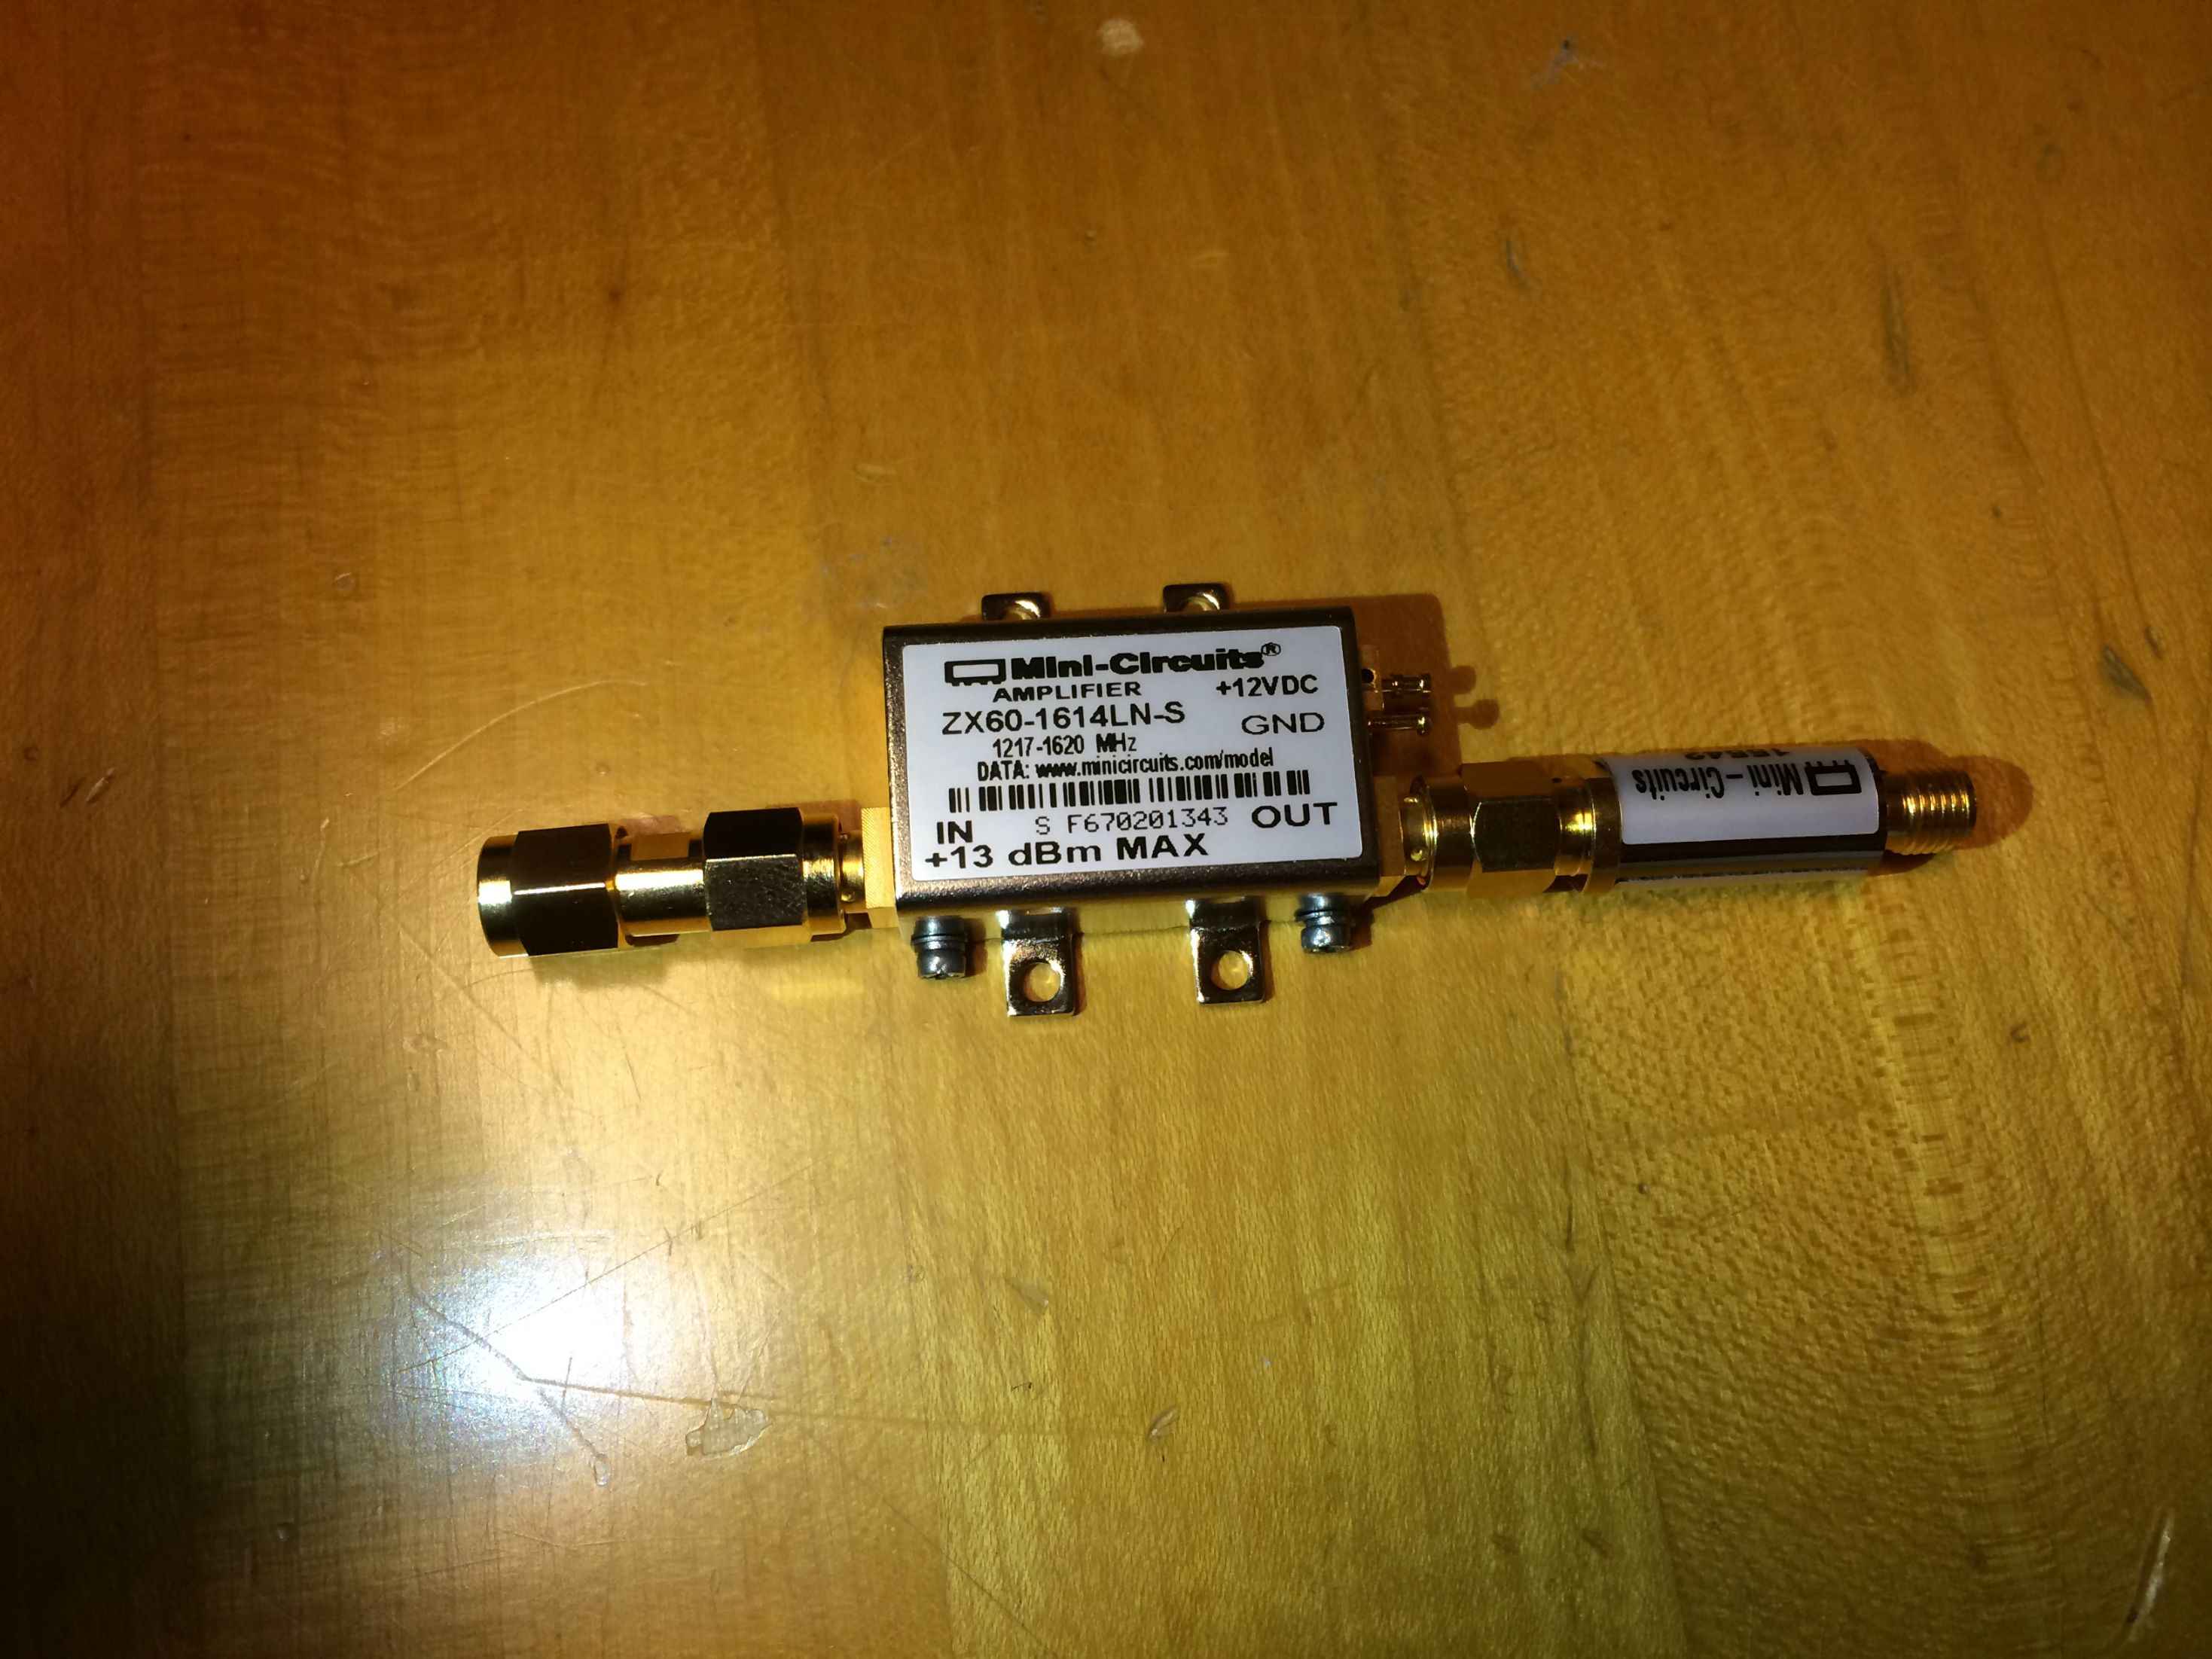
\includegraphics[scale=0.12]{lna/01.jpeg}
\end{center}

Connected one coaxial cable to bandpass. 

\begin{center}
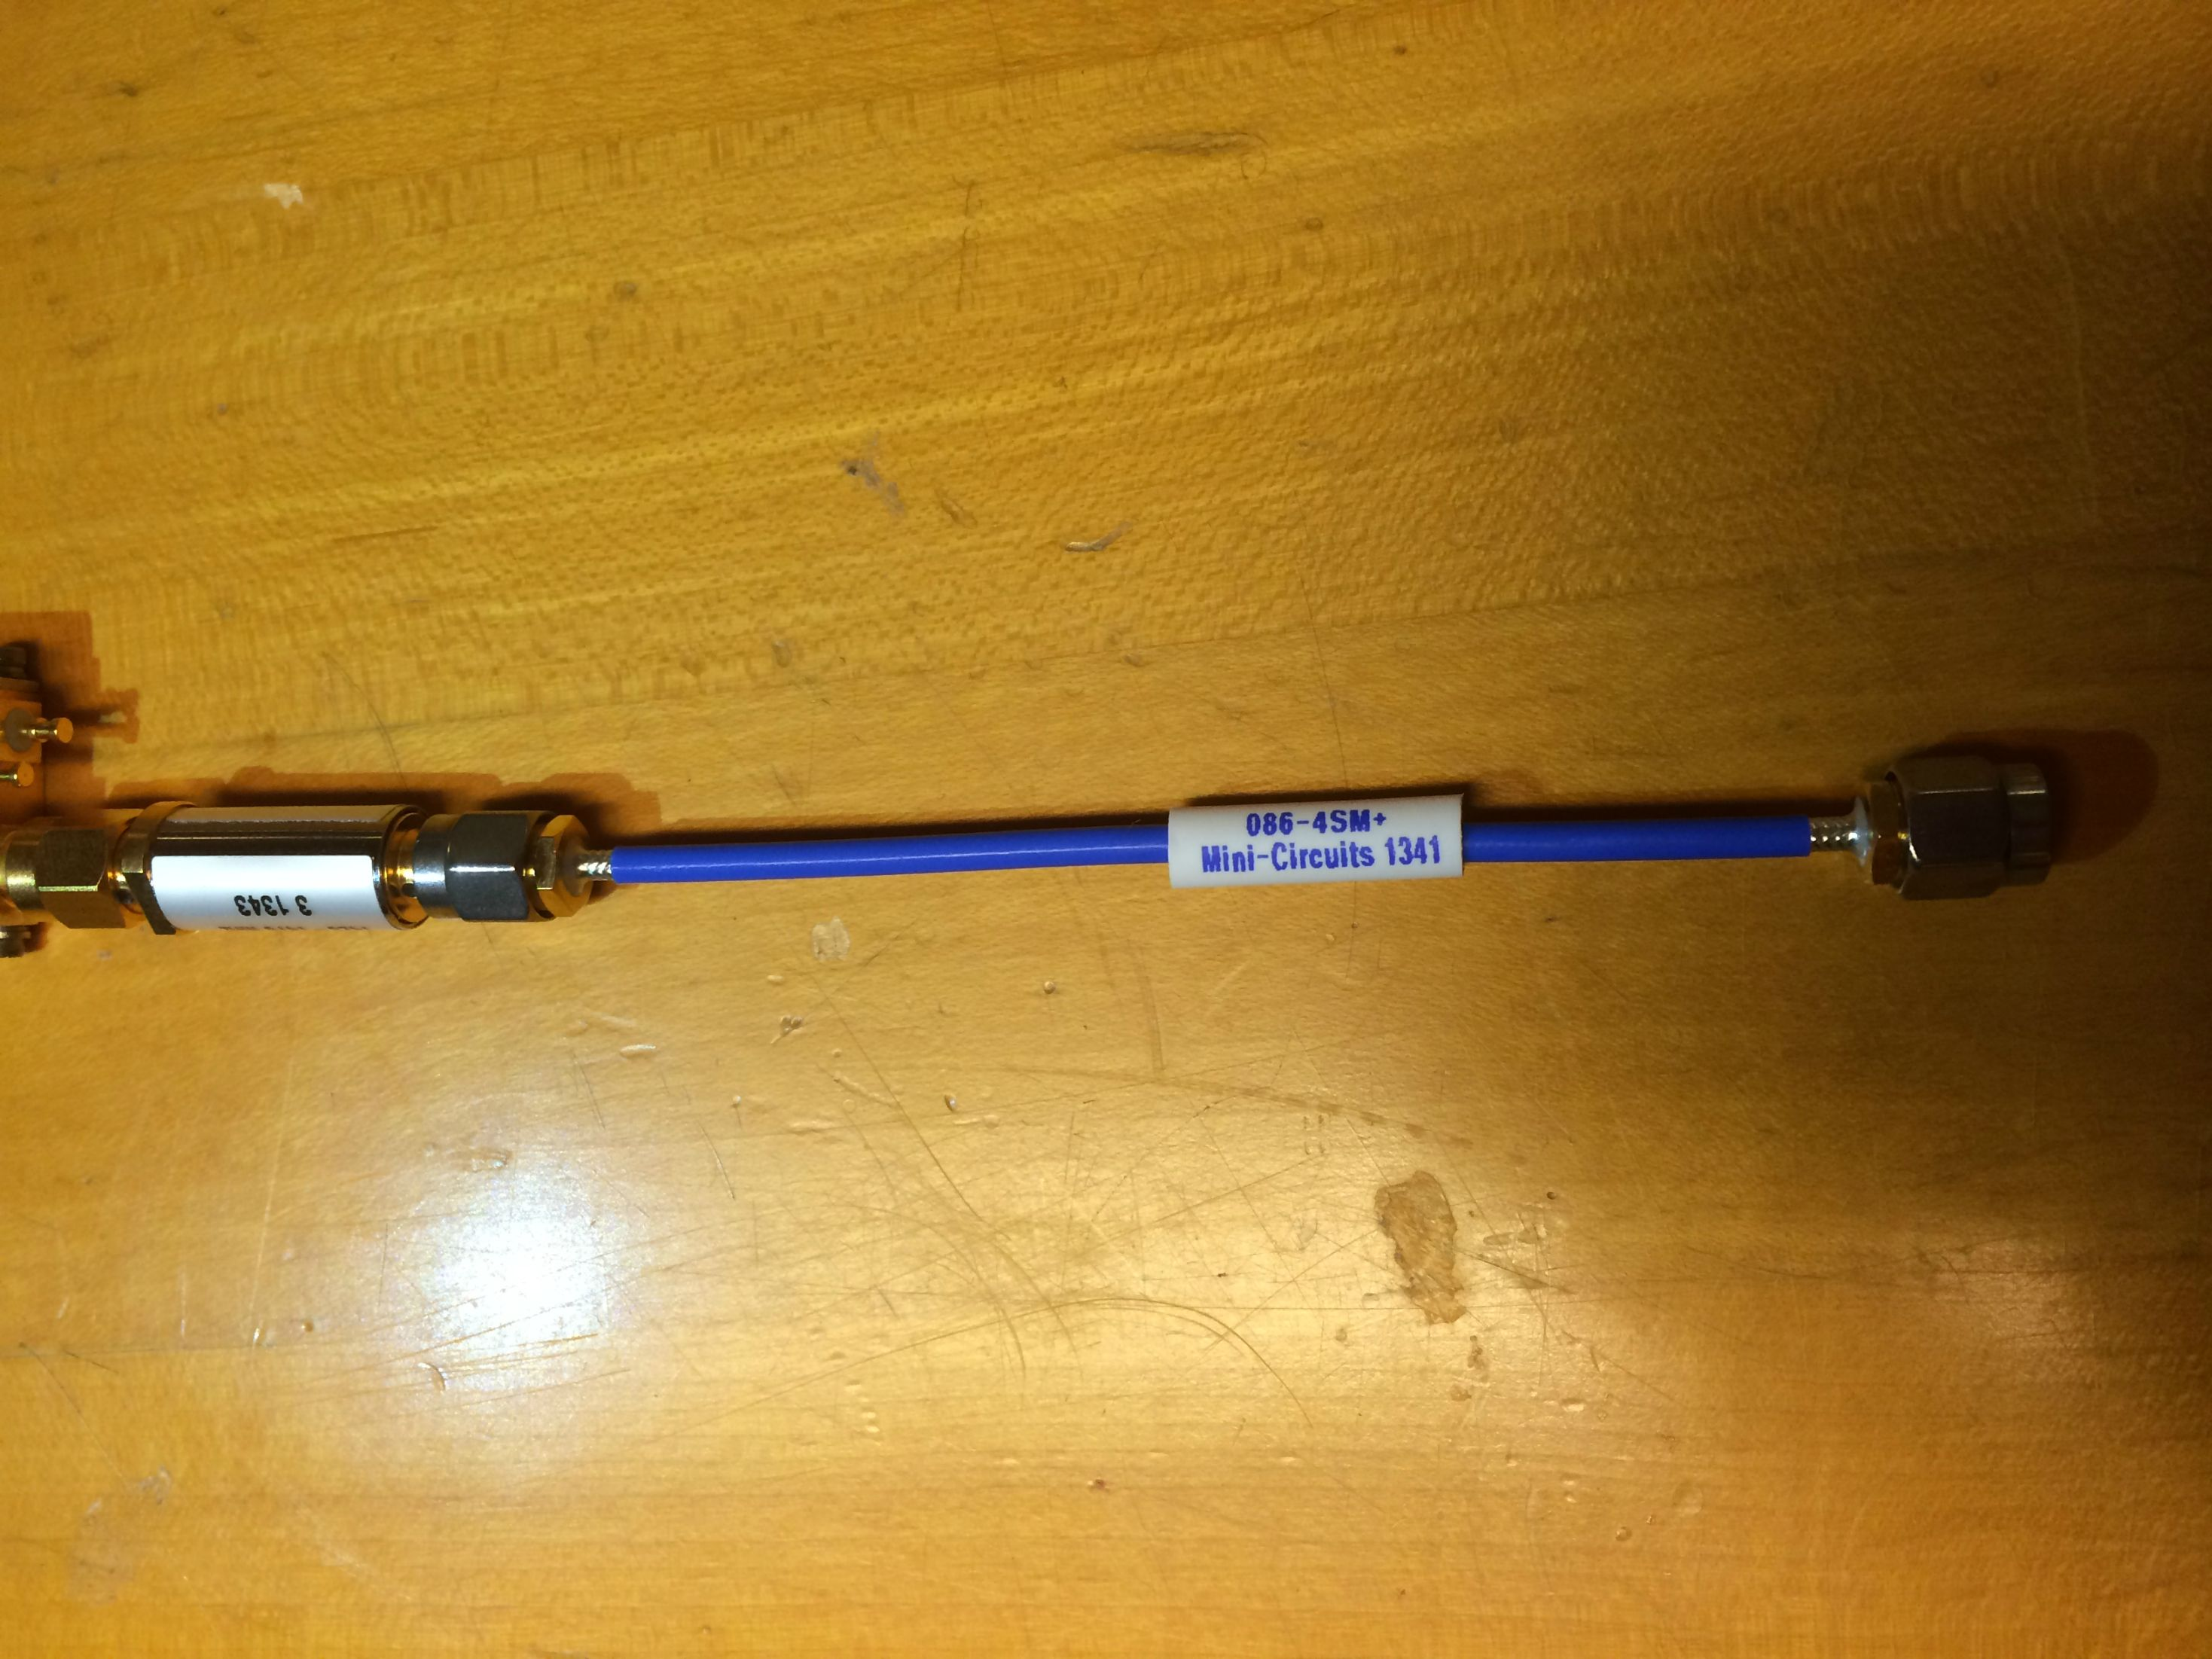
\includegraphics[scale=0.12]{lna/02.jpeg}
\end{center}

Connected opposite end of coaxial cable to "In" side of Amp 2. 

\begin{center}
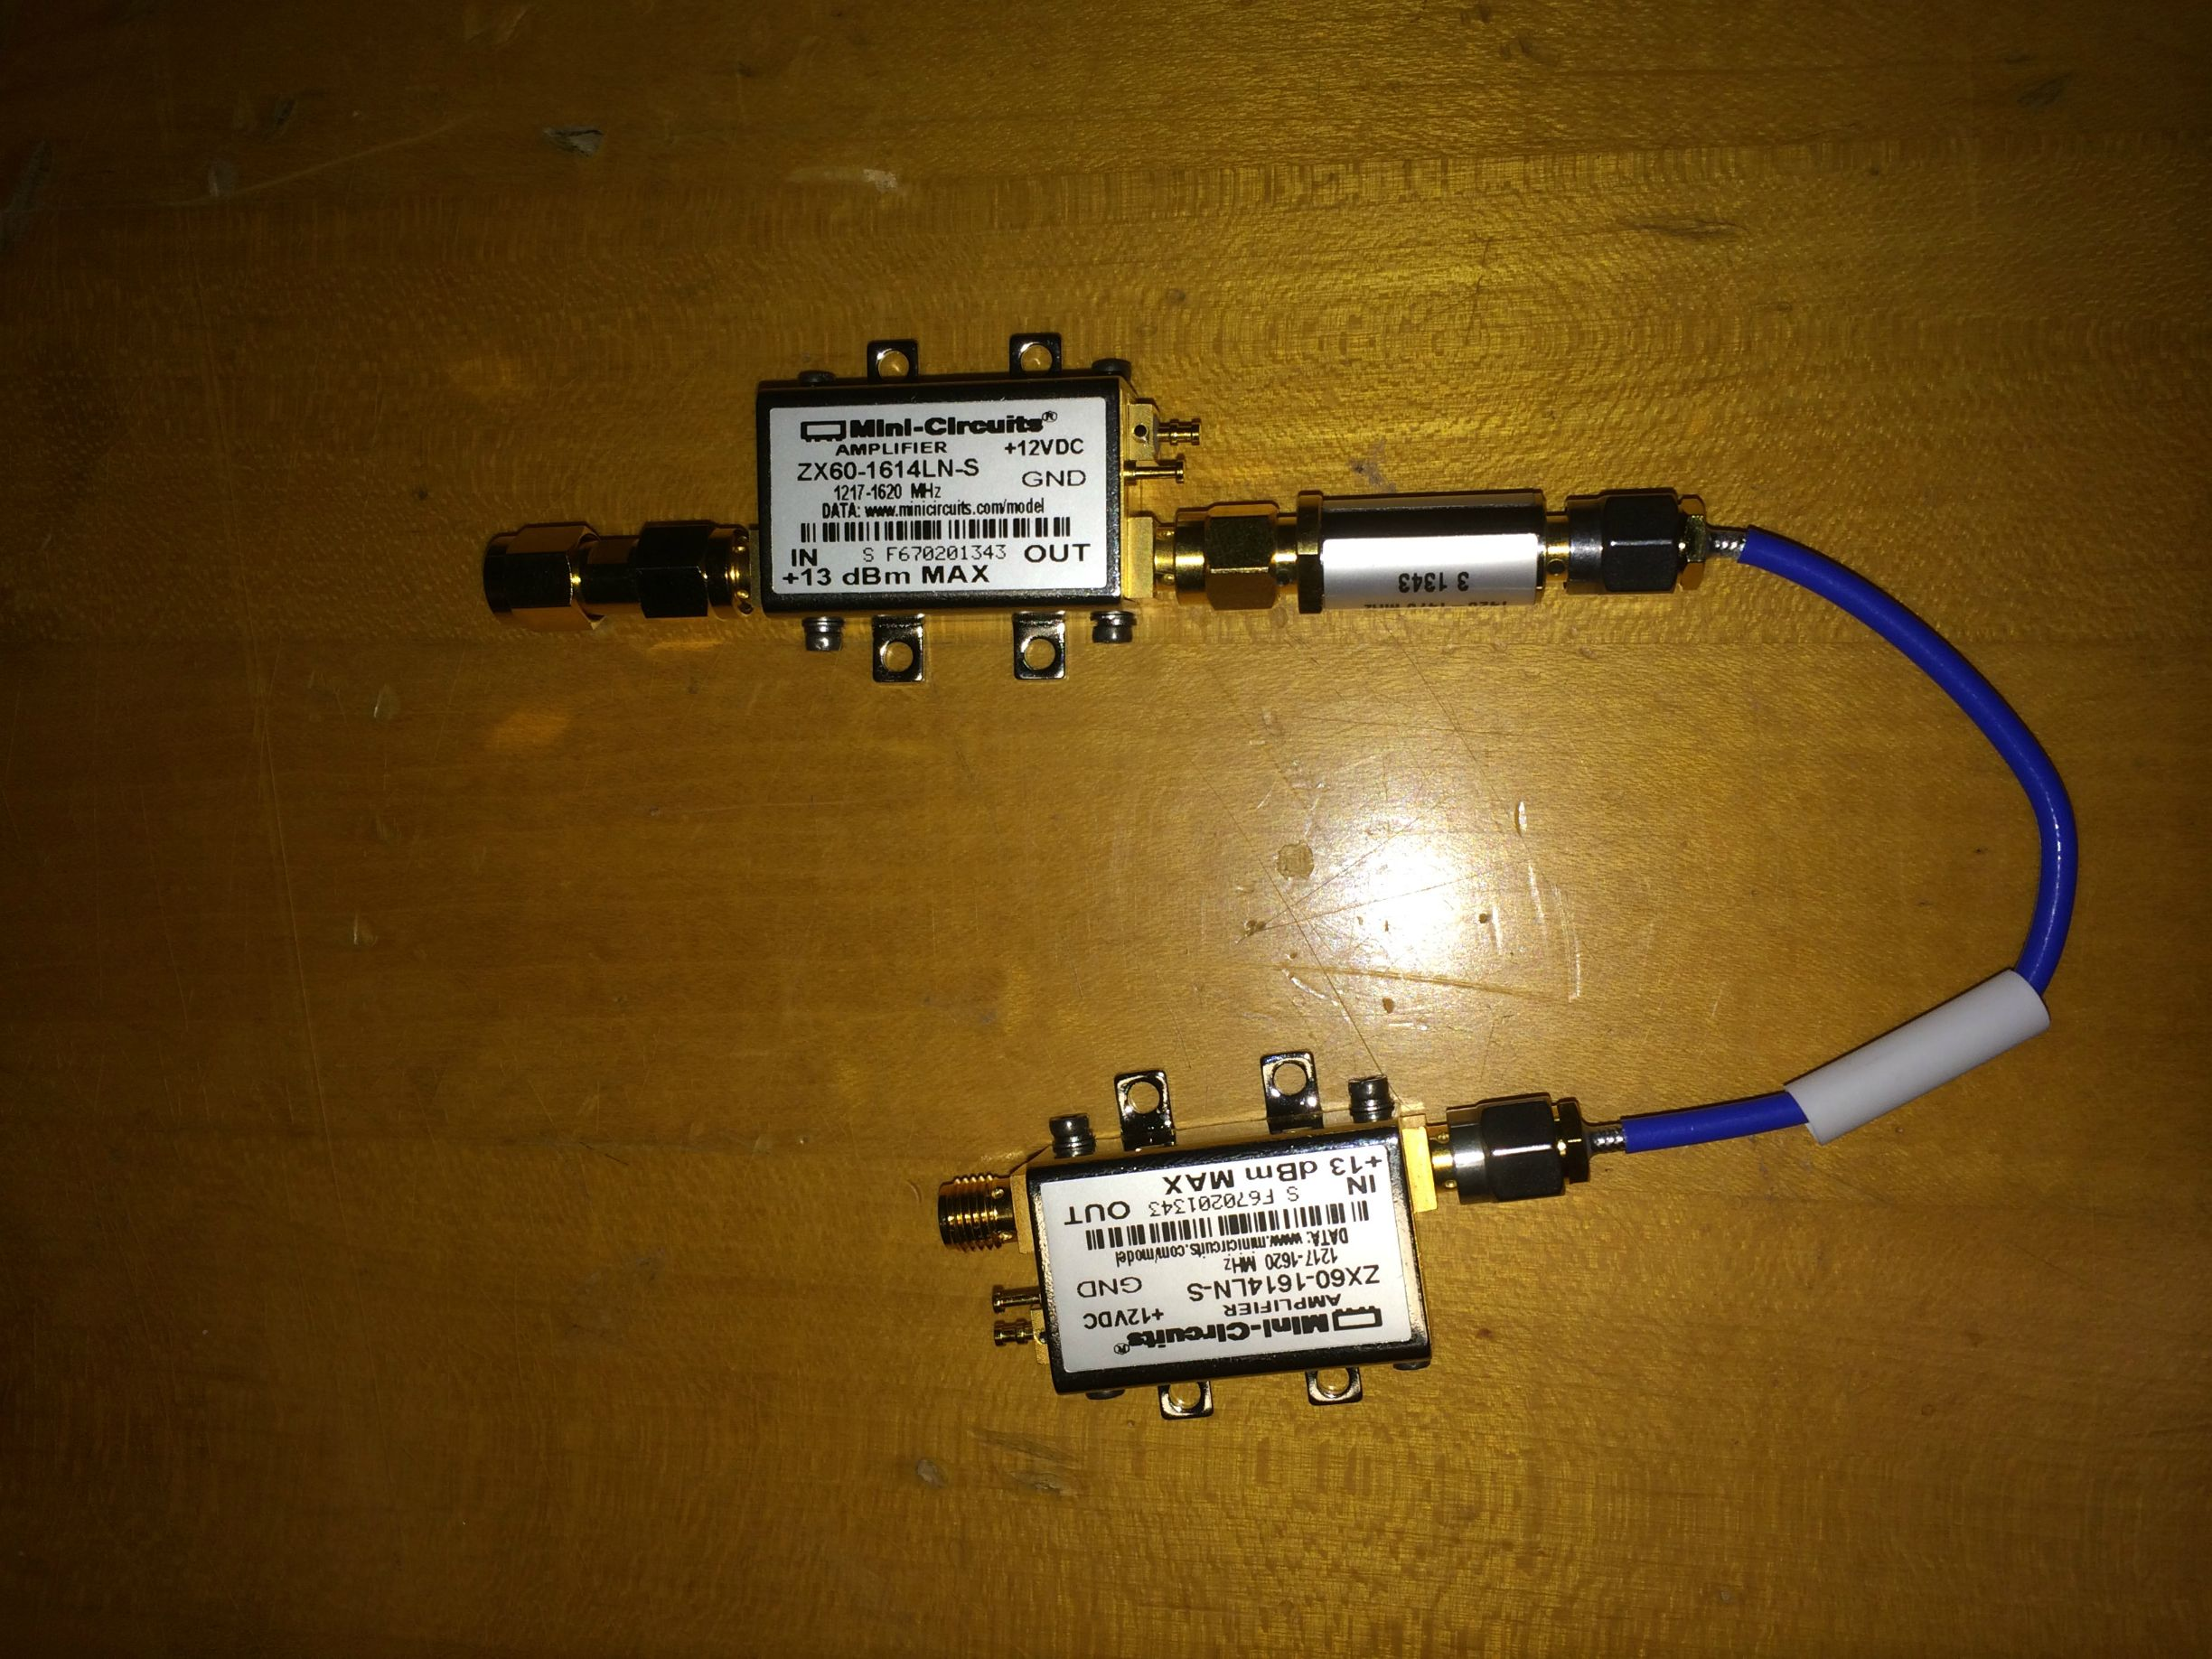
\includegraphics[scale=0.14]{lna/03.jpeg}
\end{center}

Cut two lengths of 15-20 centimeter long 22 gauge copper wire. 
Soldered one wire to both Amps.
Soldered the other wire to Amp 2. 

\begin{center}
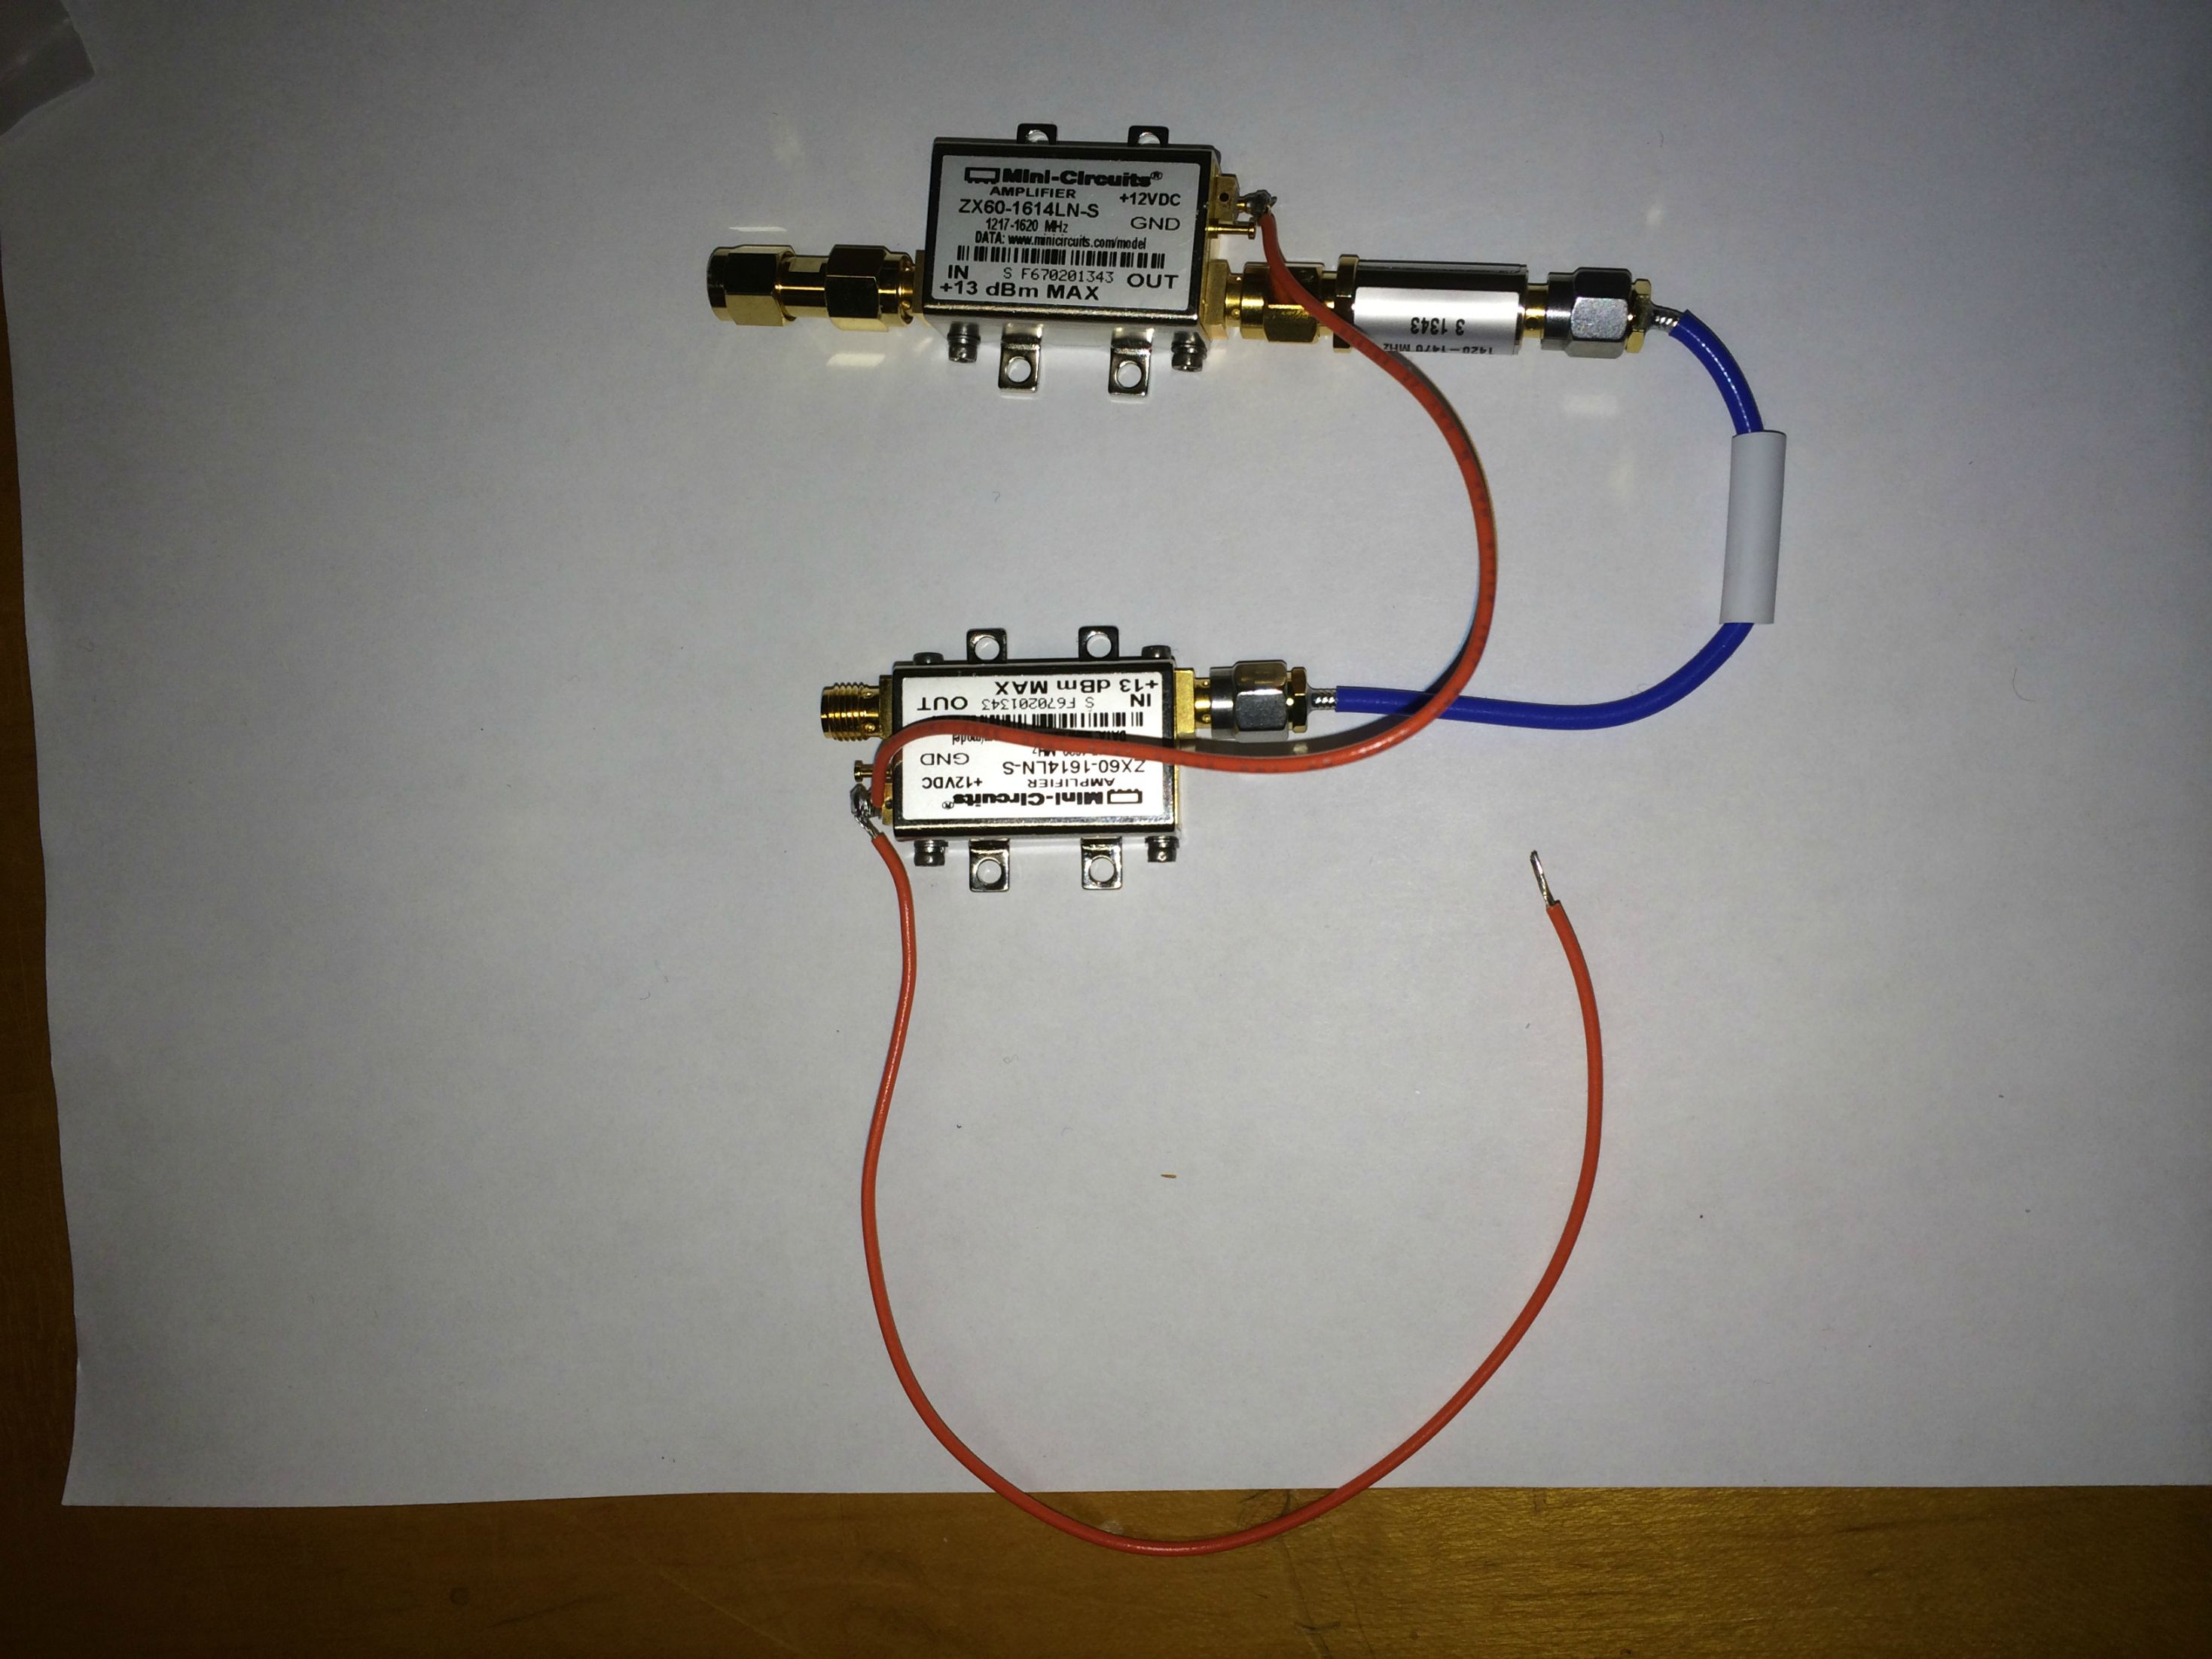
\includegraphics[scale=0.13]{lna/04.jpeg}
\end{center}

Soldered the other end of the second wire to the 12 volt pin on the bias tee.
Connected "RF" side of the bias tee and "out" side of Amp 2 with coaxial cable. 

\begin{center}
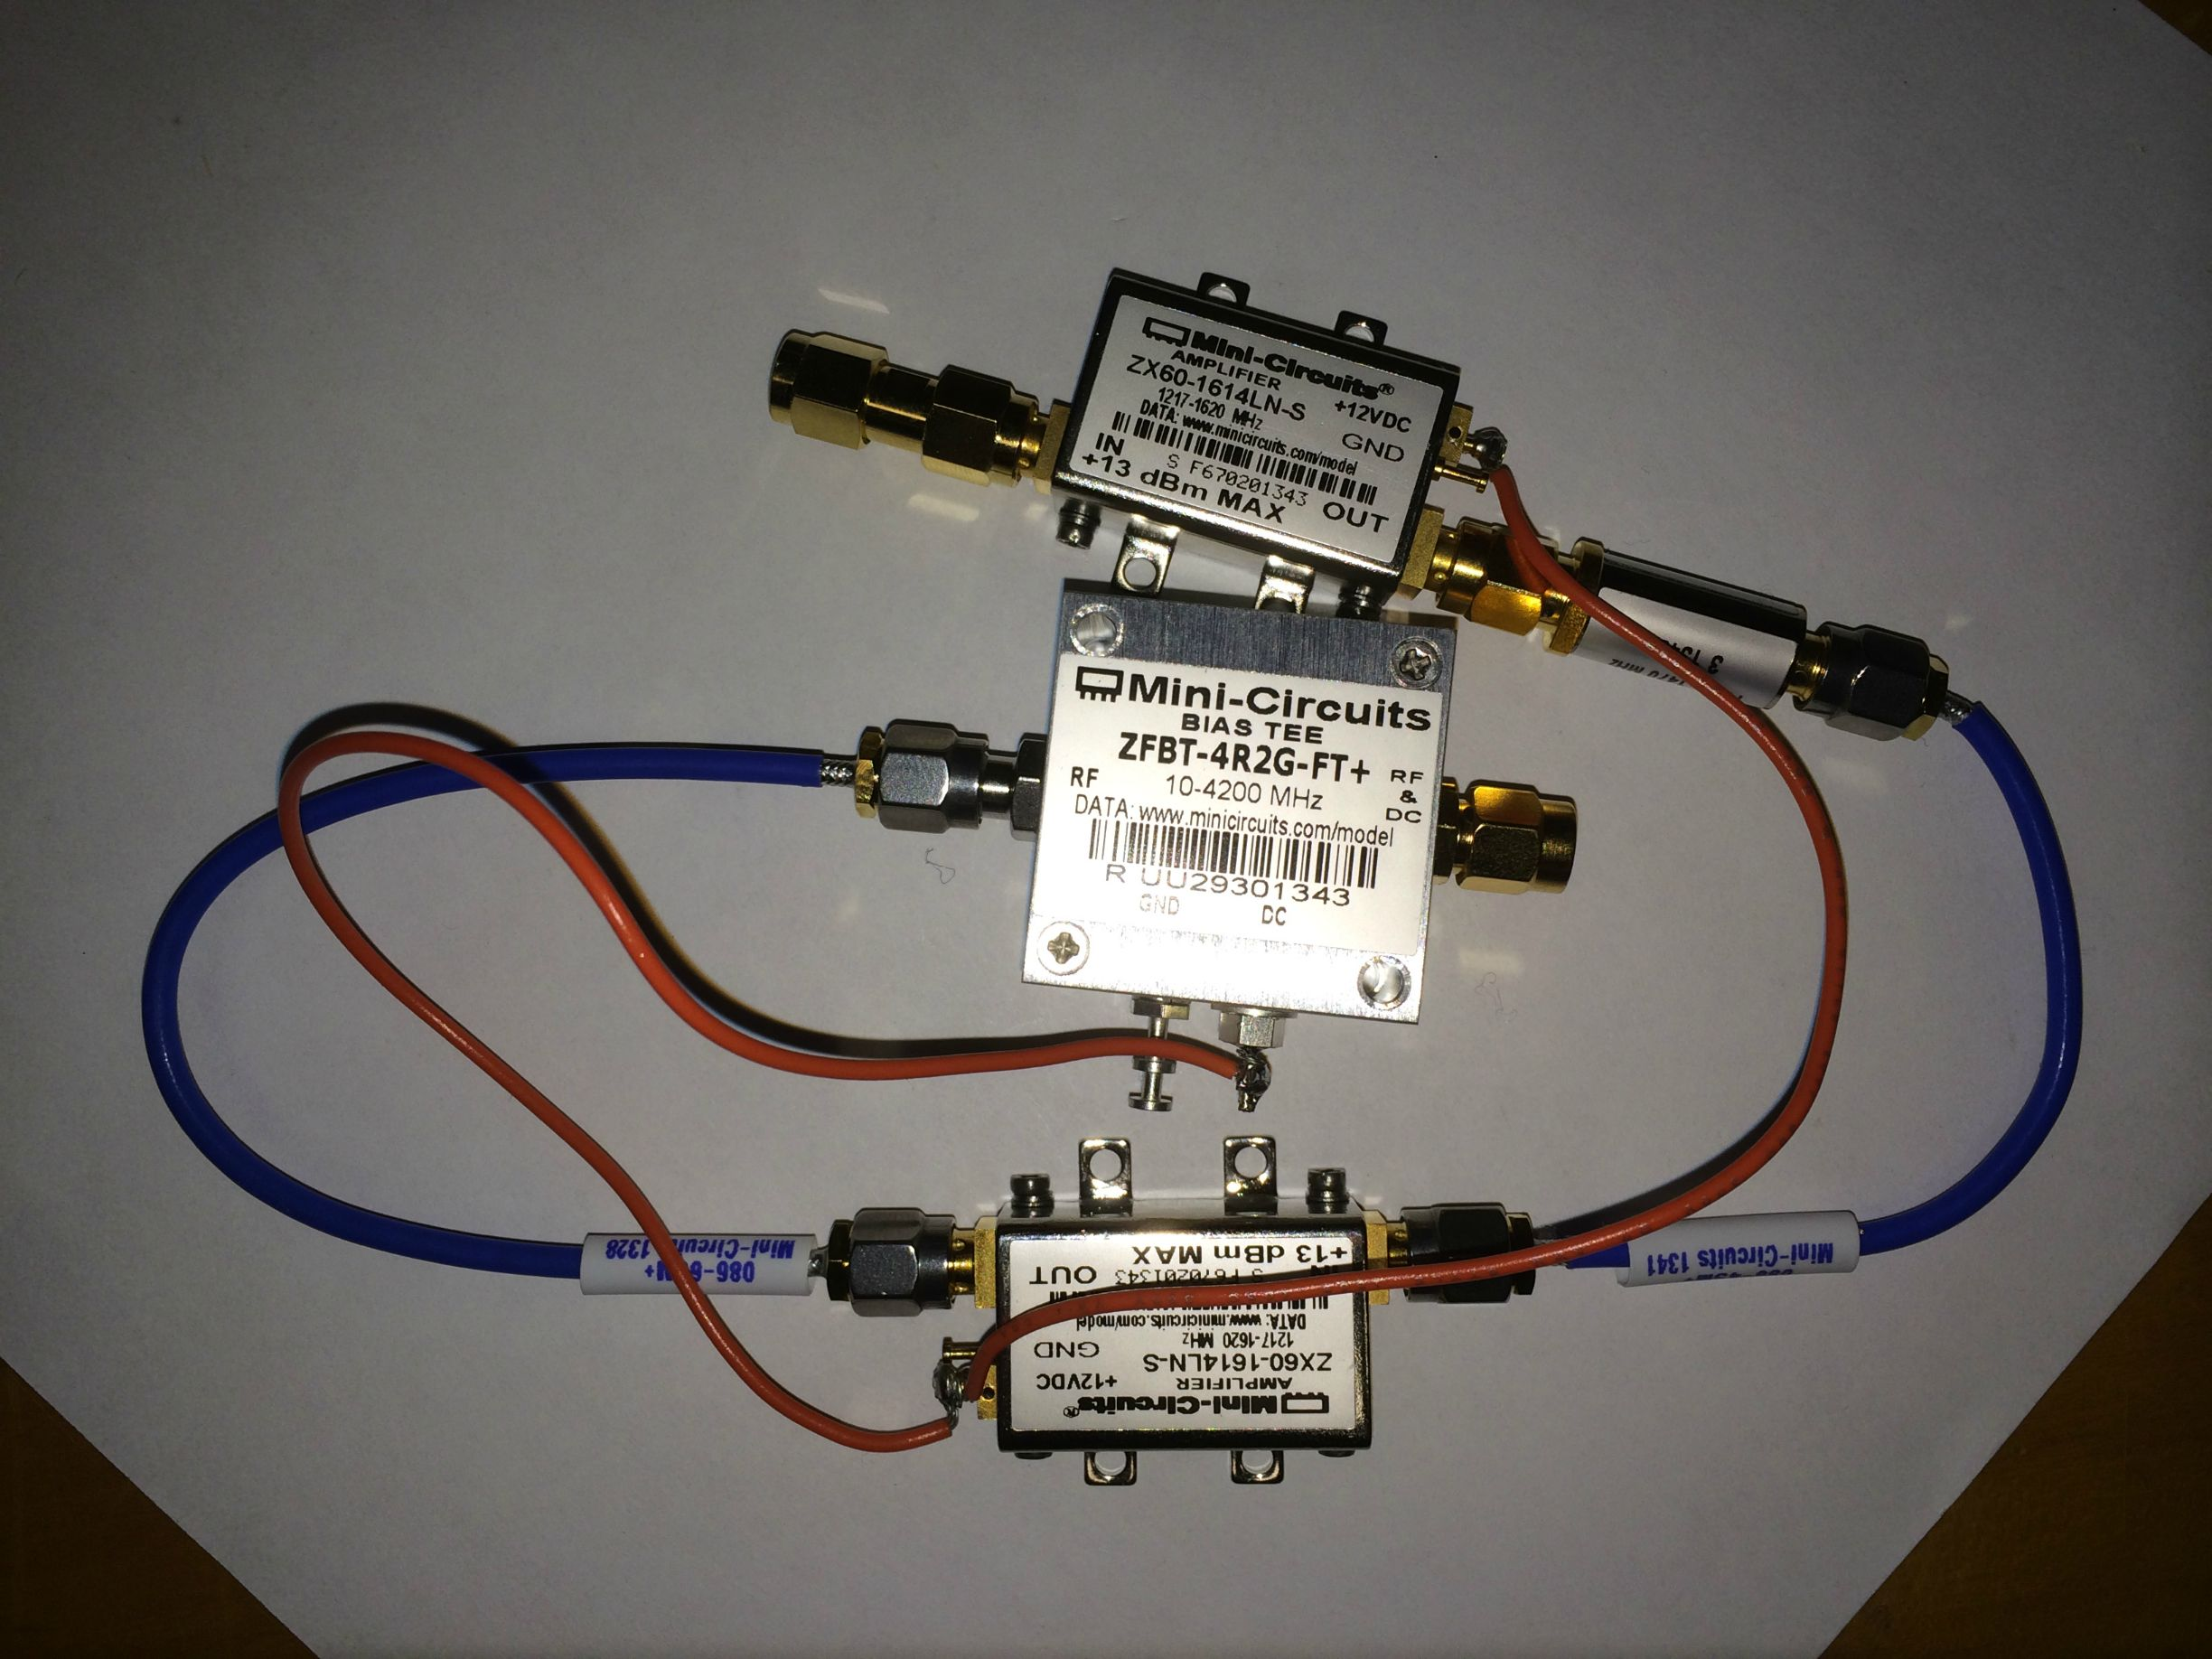
\includegraphics[scale=0.15]{lna/05.jpeg}
\end{center}

Placed this group into the case, with coupler and "RF DC" side of the bias tee protruding from the holes. 

\begin{center}
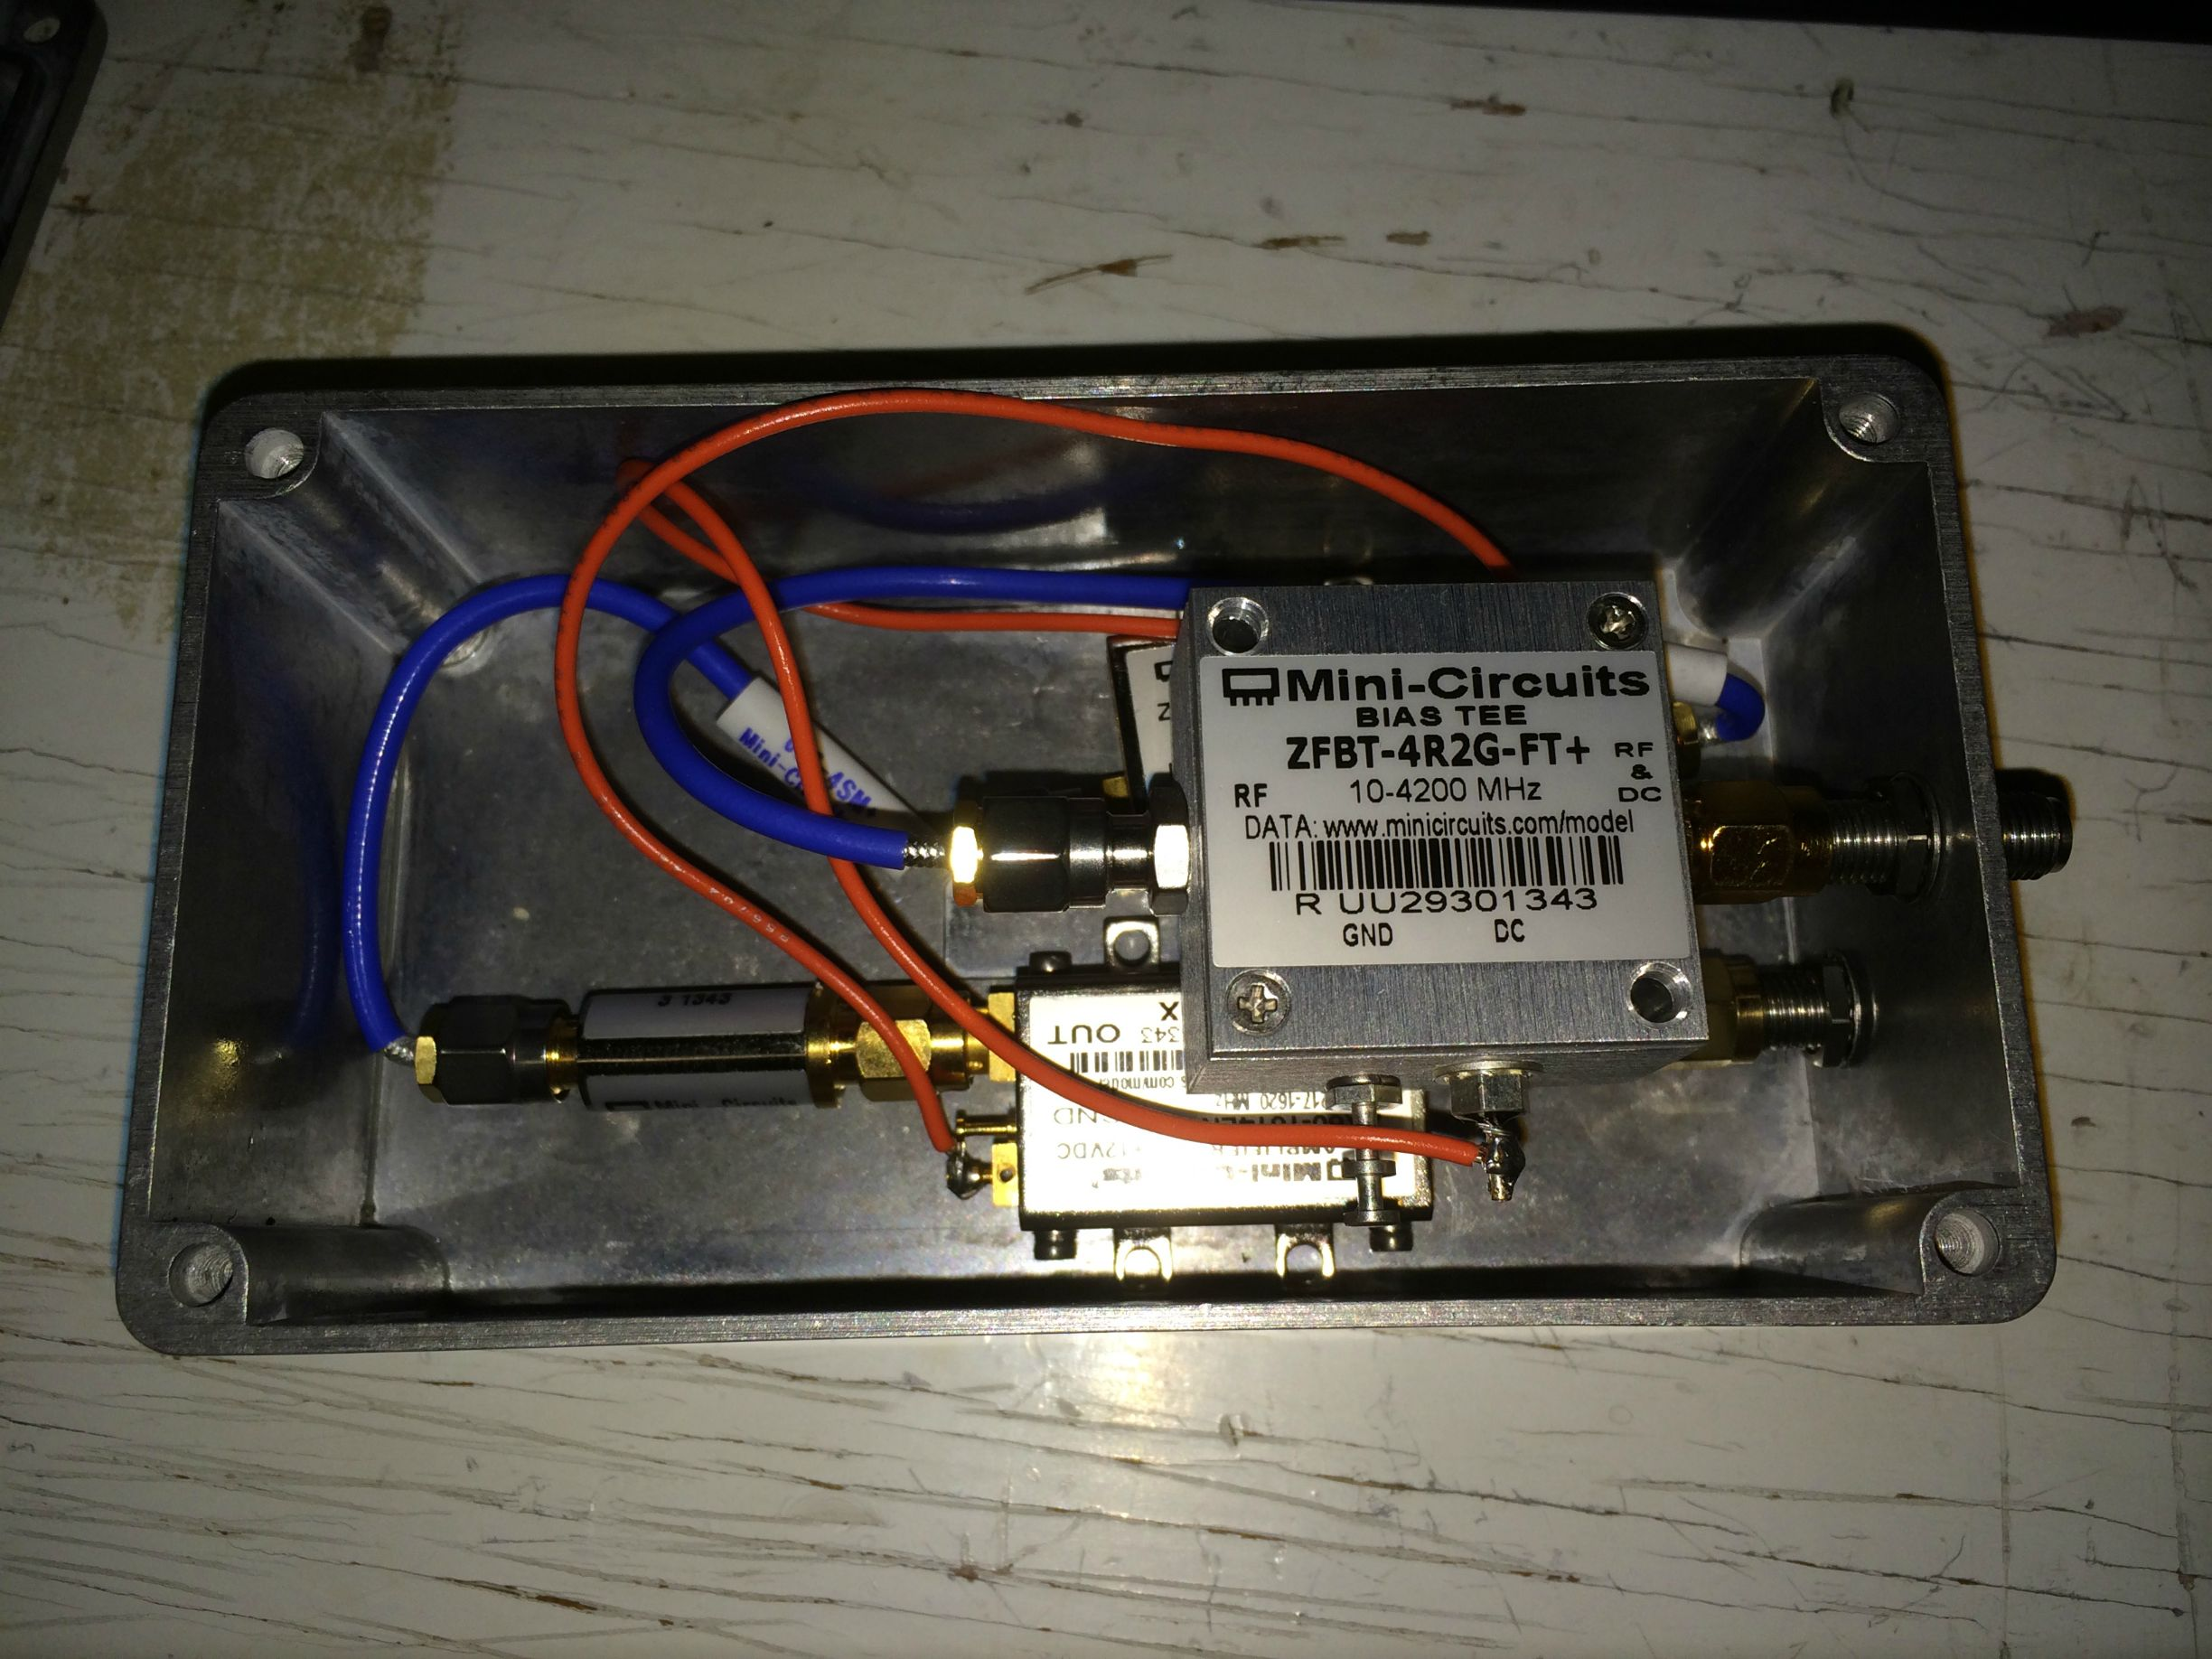
\includegraphics[scale=0.12]{lna/06.jpeg}
\end{center}

Placed on rubber lining, and case cover, wrote LNA on top, and screwed into place. 

\begin{center}
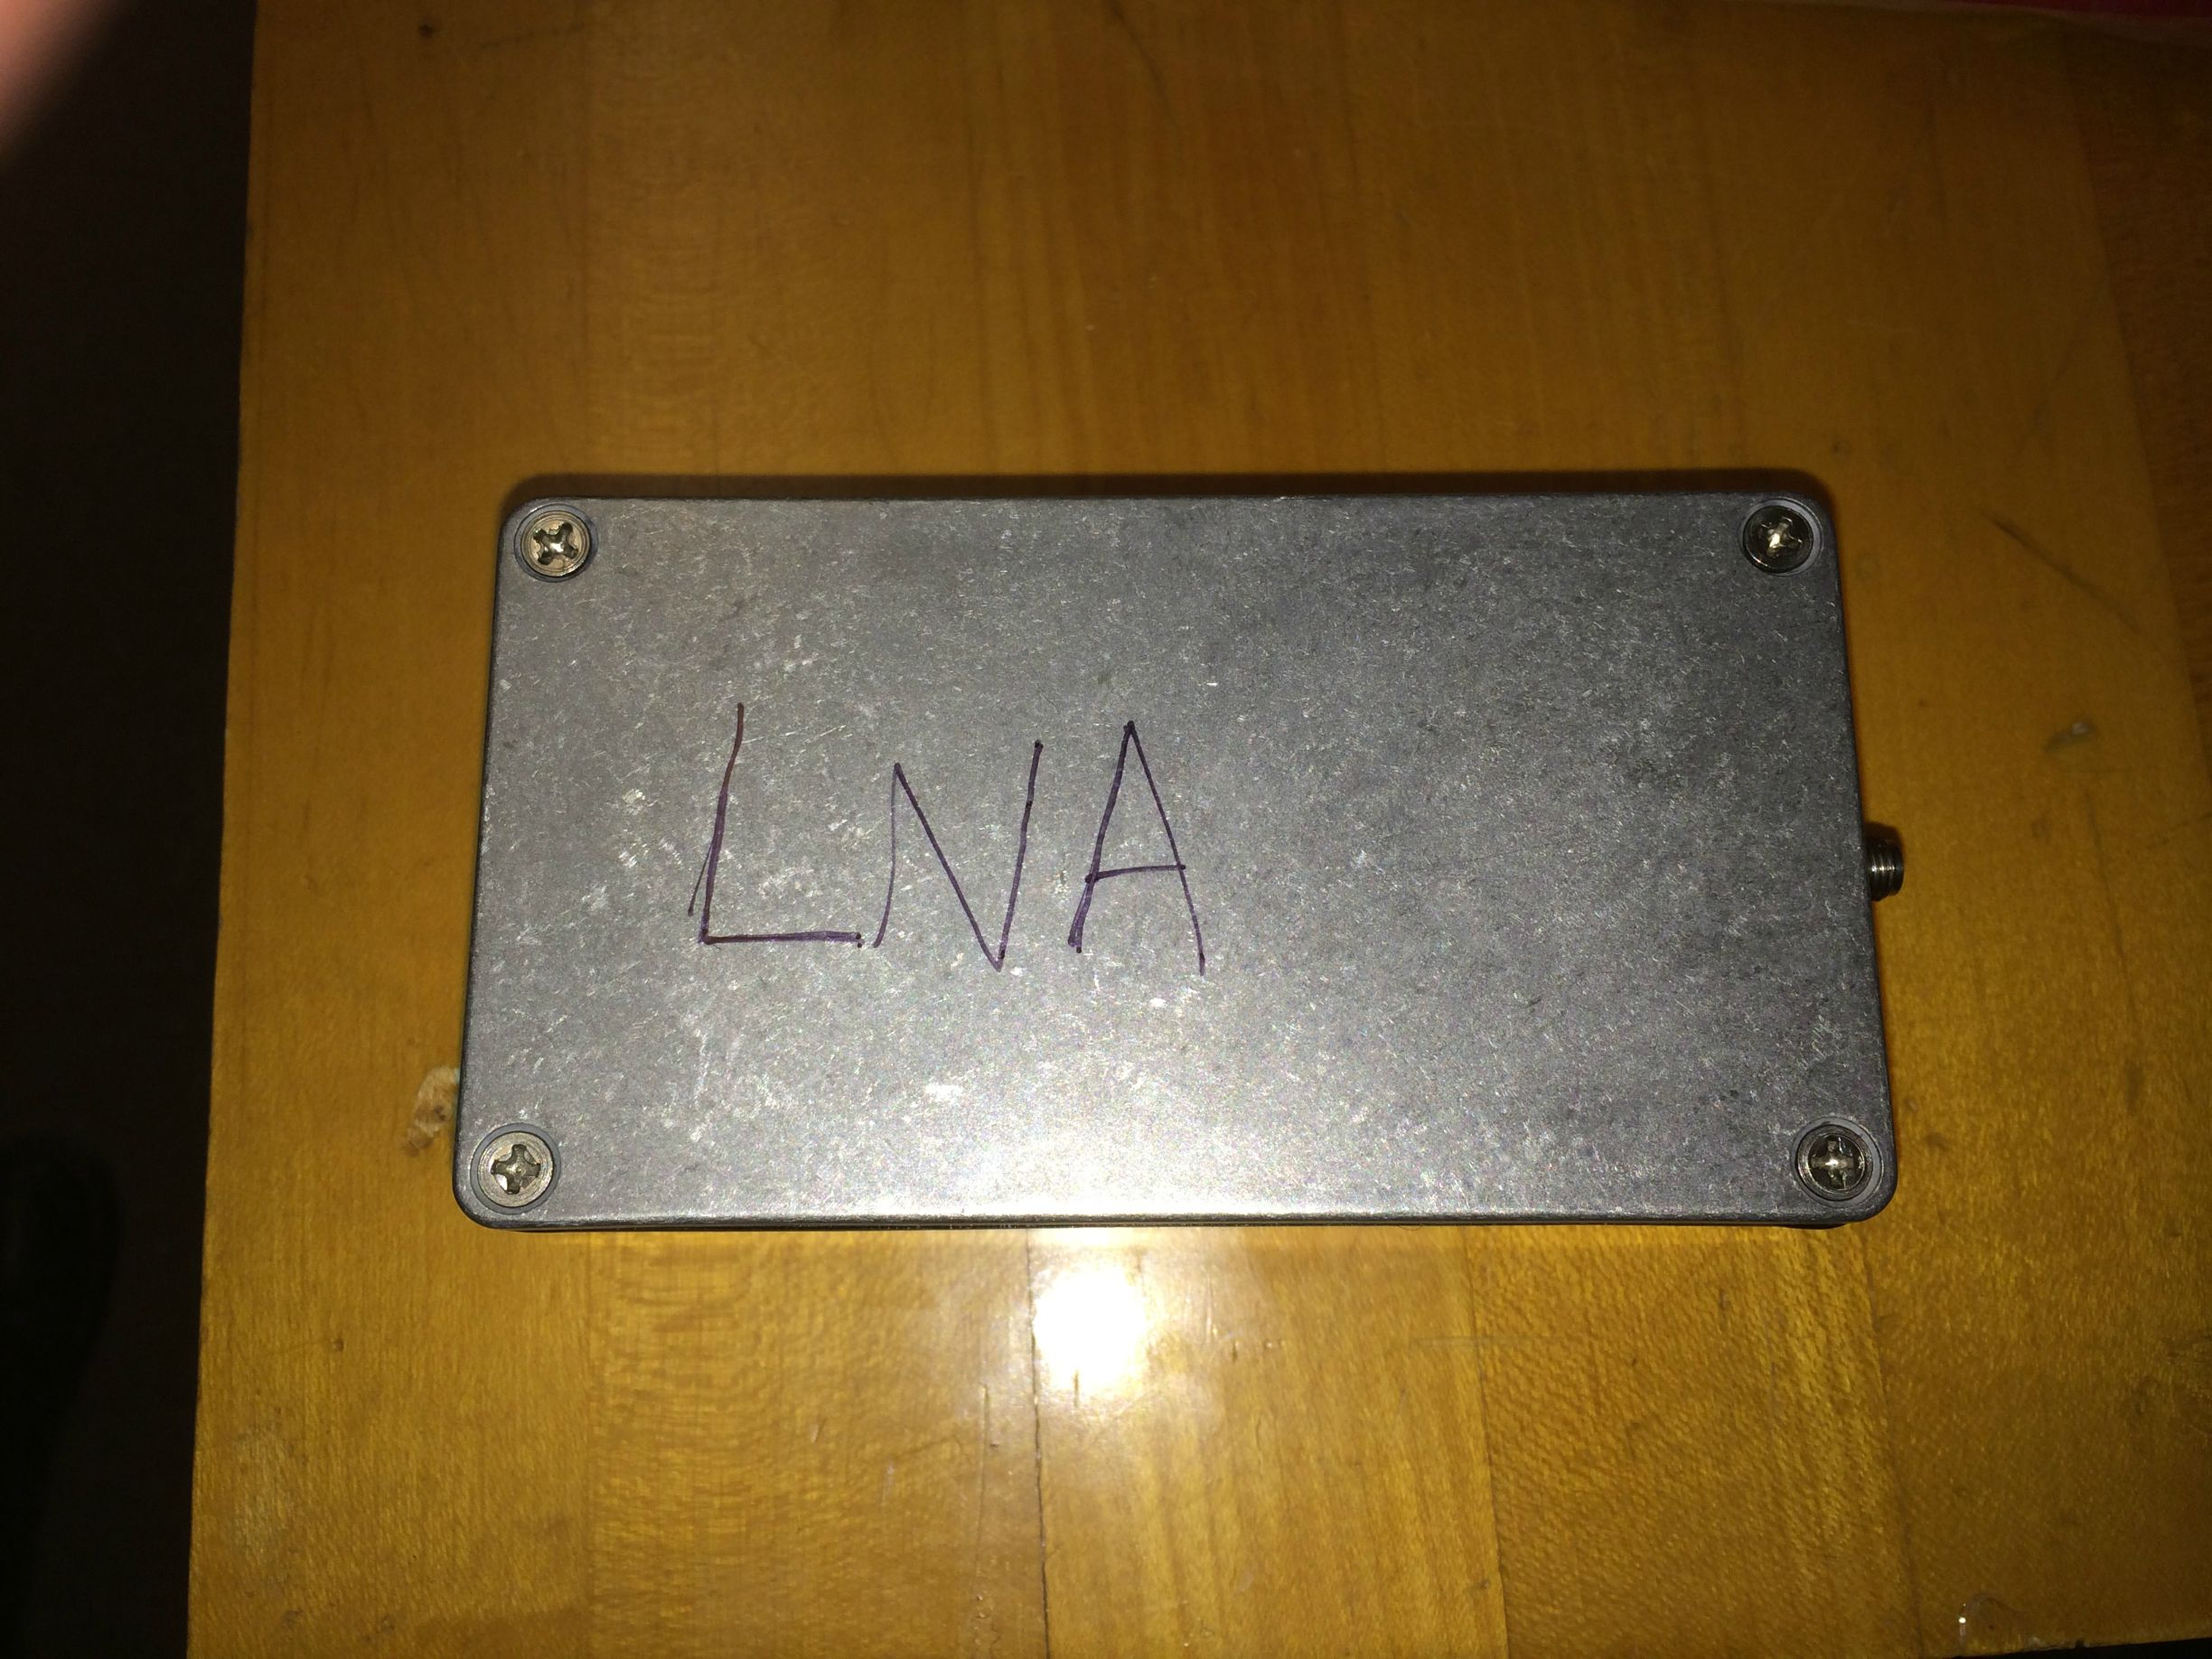
\includegraphics[scale=0.12]{lna/07.jpeg}
\end{center}

Pics of assembly of dc jack connector to f type coax adapter.
Solder middle pin of dc plug connector to perf board.
Solder middle pin of f type plug connector to same conductive strip of perf board. 

\begin{center}
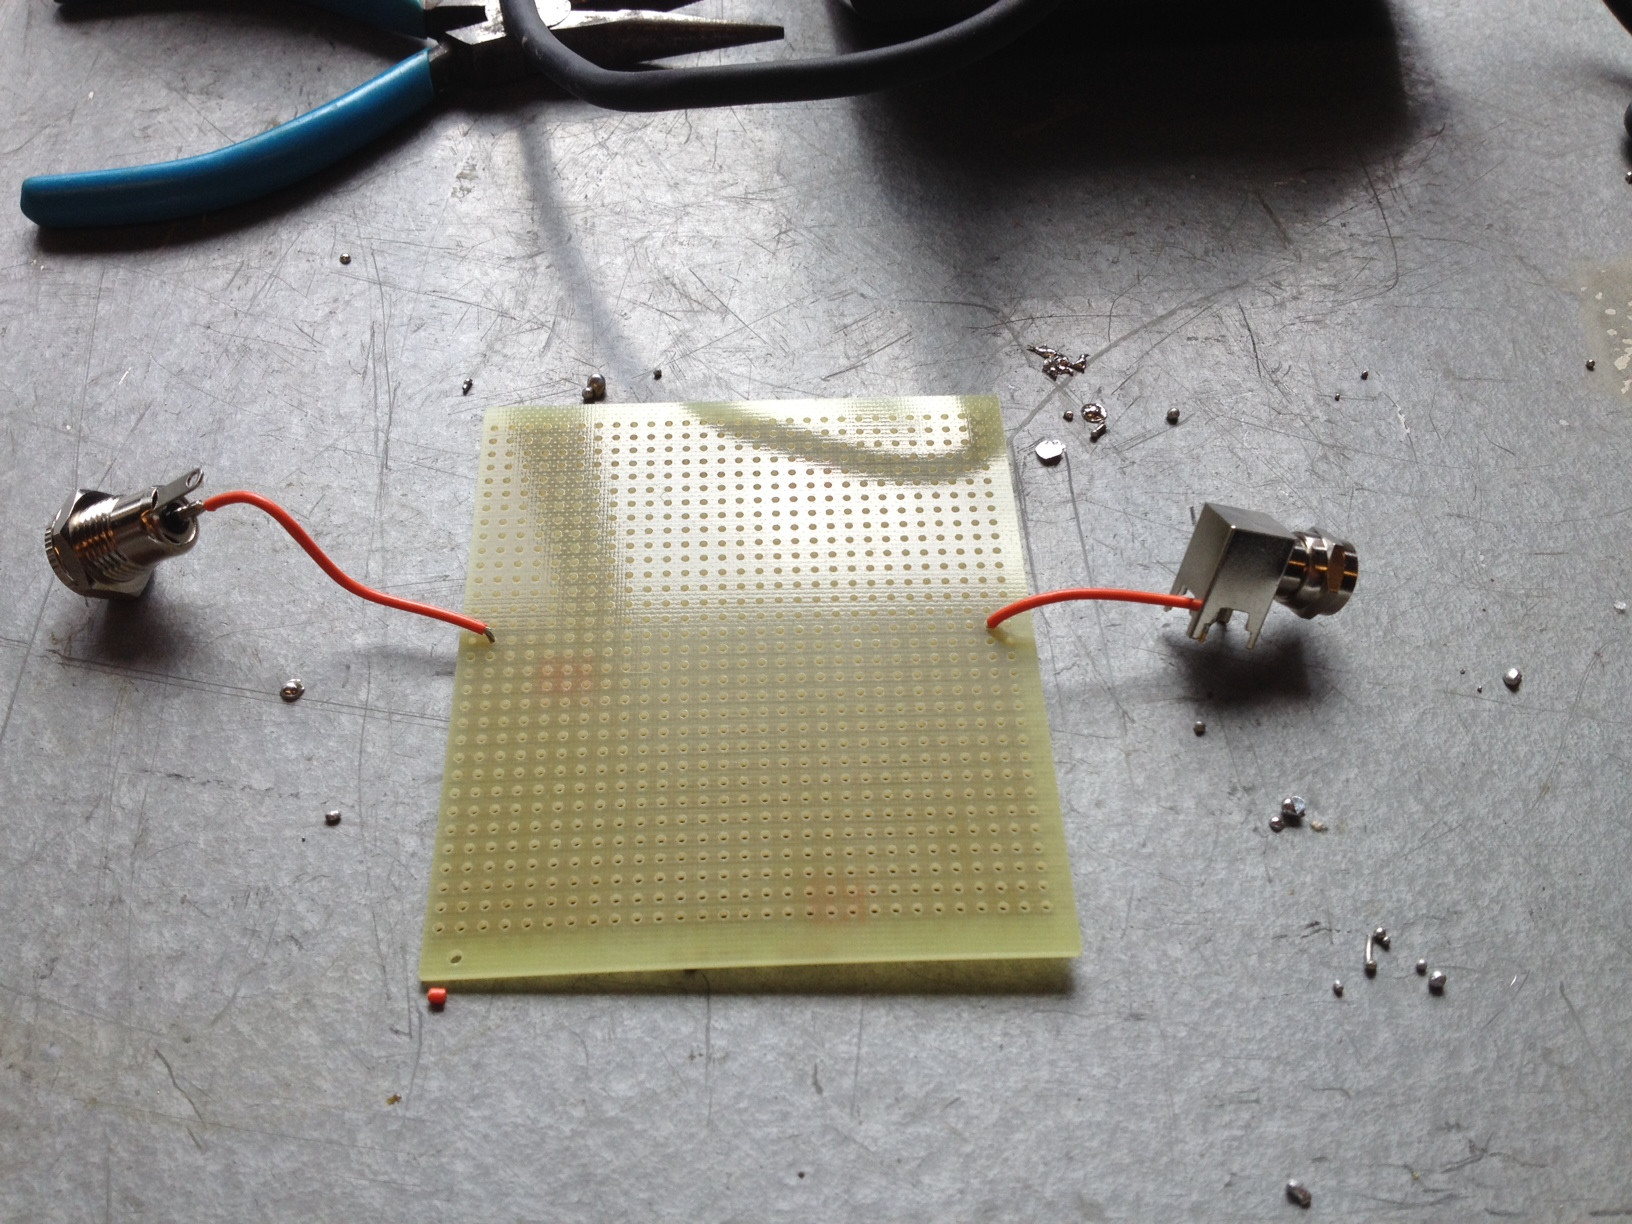
\includegraphics[scale=0.20]{lna/08.jpeg}
\end{center}

Under side. 

\begin{center}
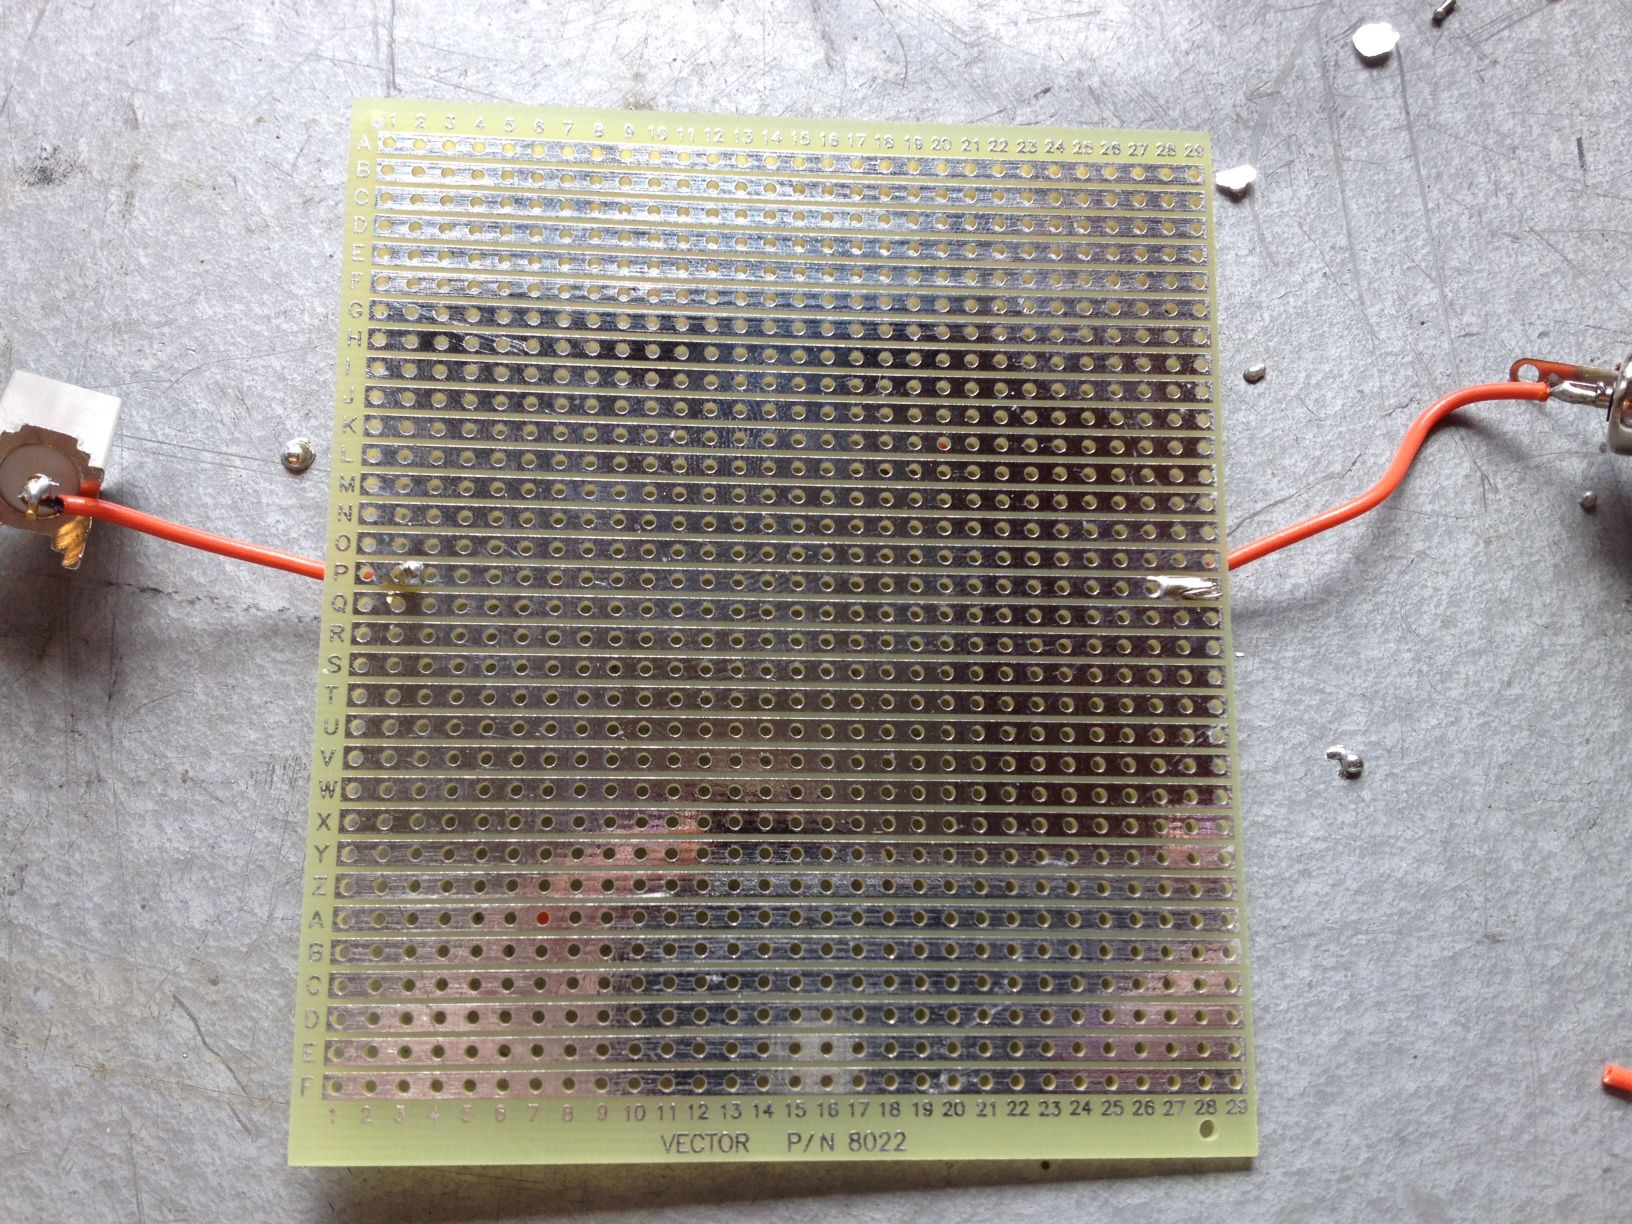
\includegraphics[scale=0.20]{lna/09.jpeg}
\end{center}

Solder ground pin on dc jack connector directly to one of the ground pins on the f type plug connector. 

\begin{center}
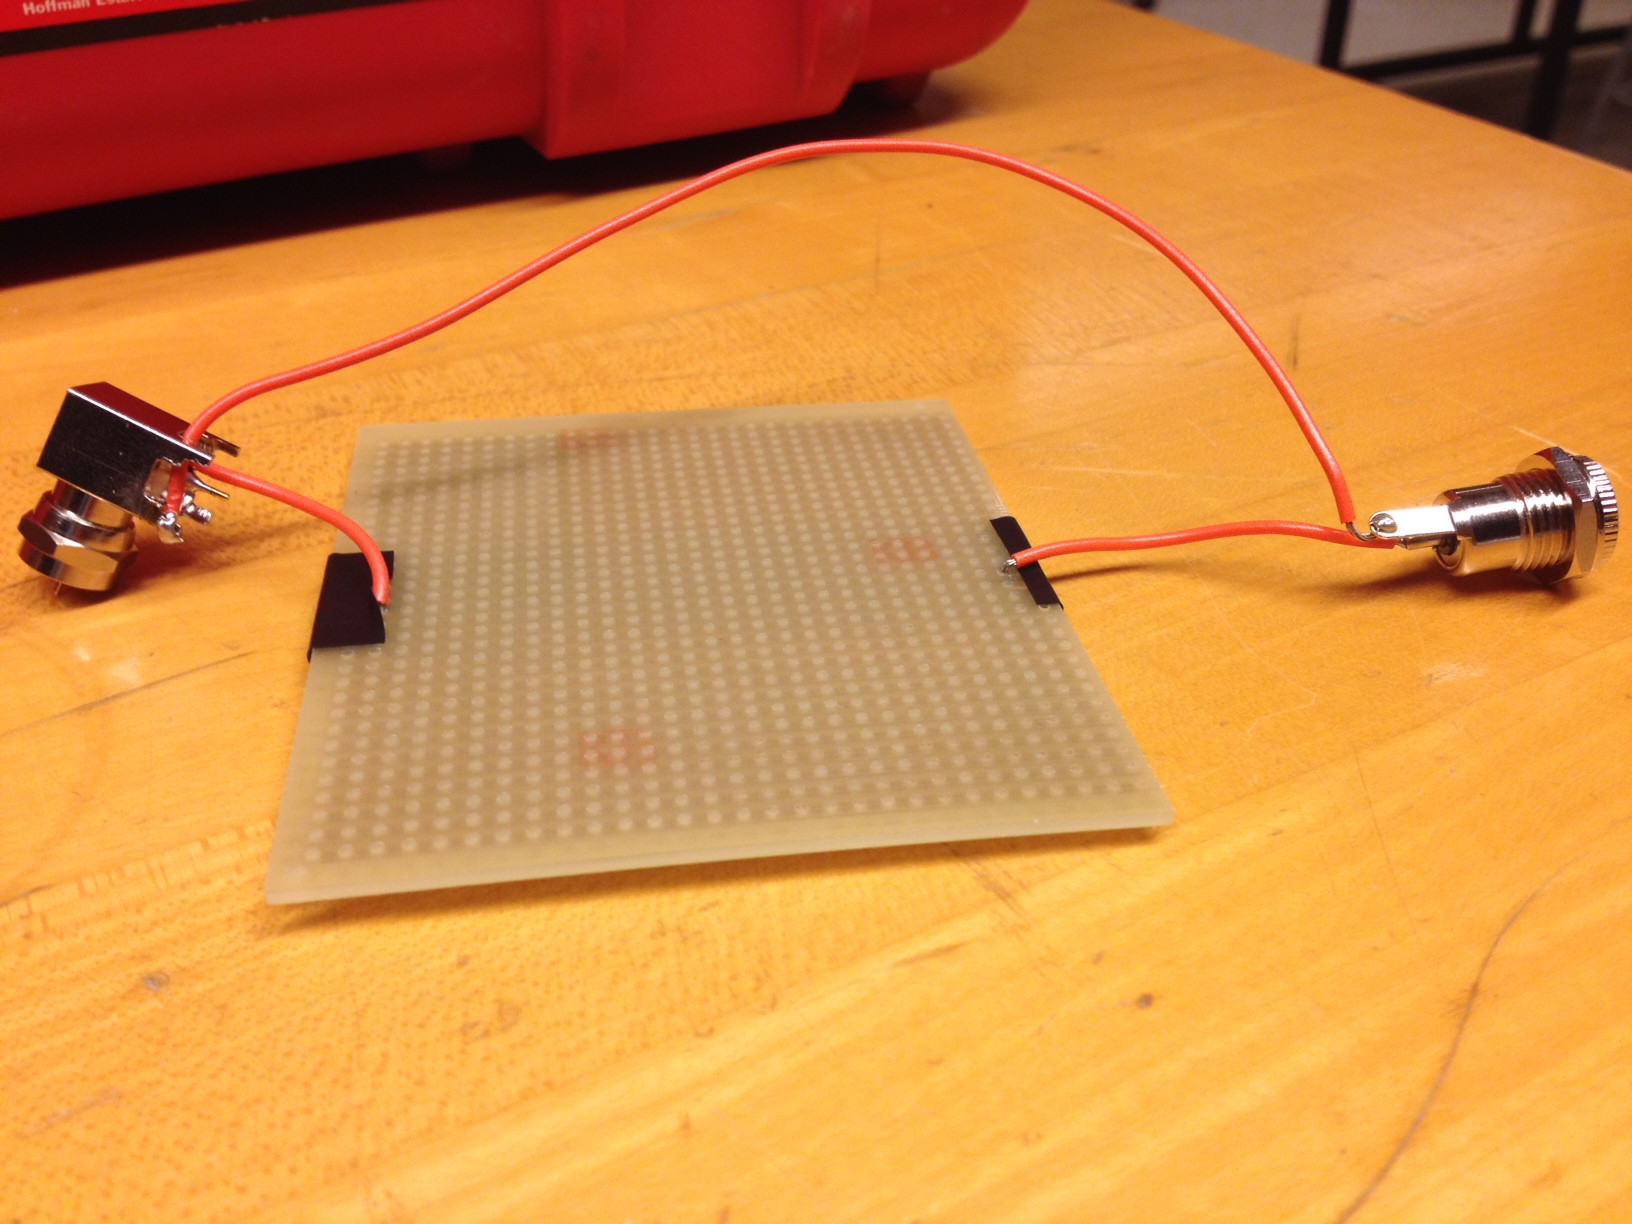
\includegraphics[scale=0.20]{lna/10.jpeg}
\end{center}

Back End b/t Dongle and LNA Put Together 

\begin{center}
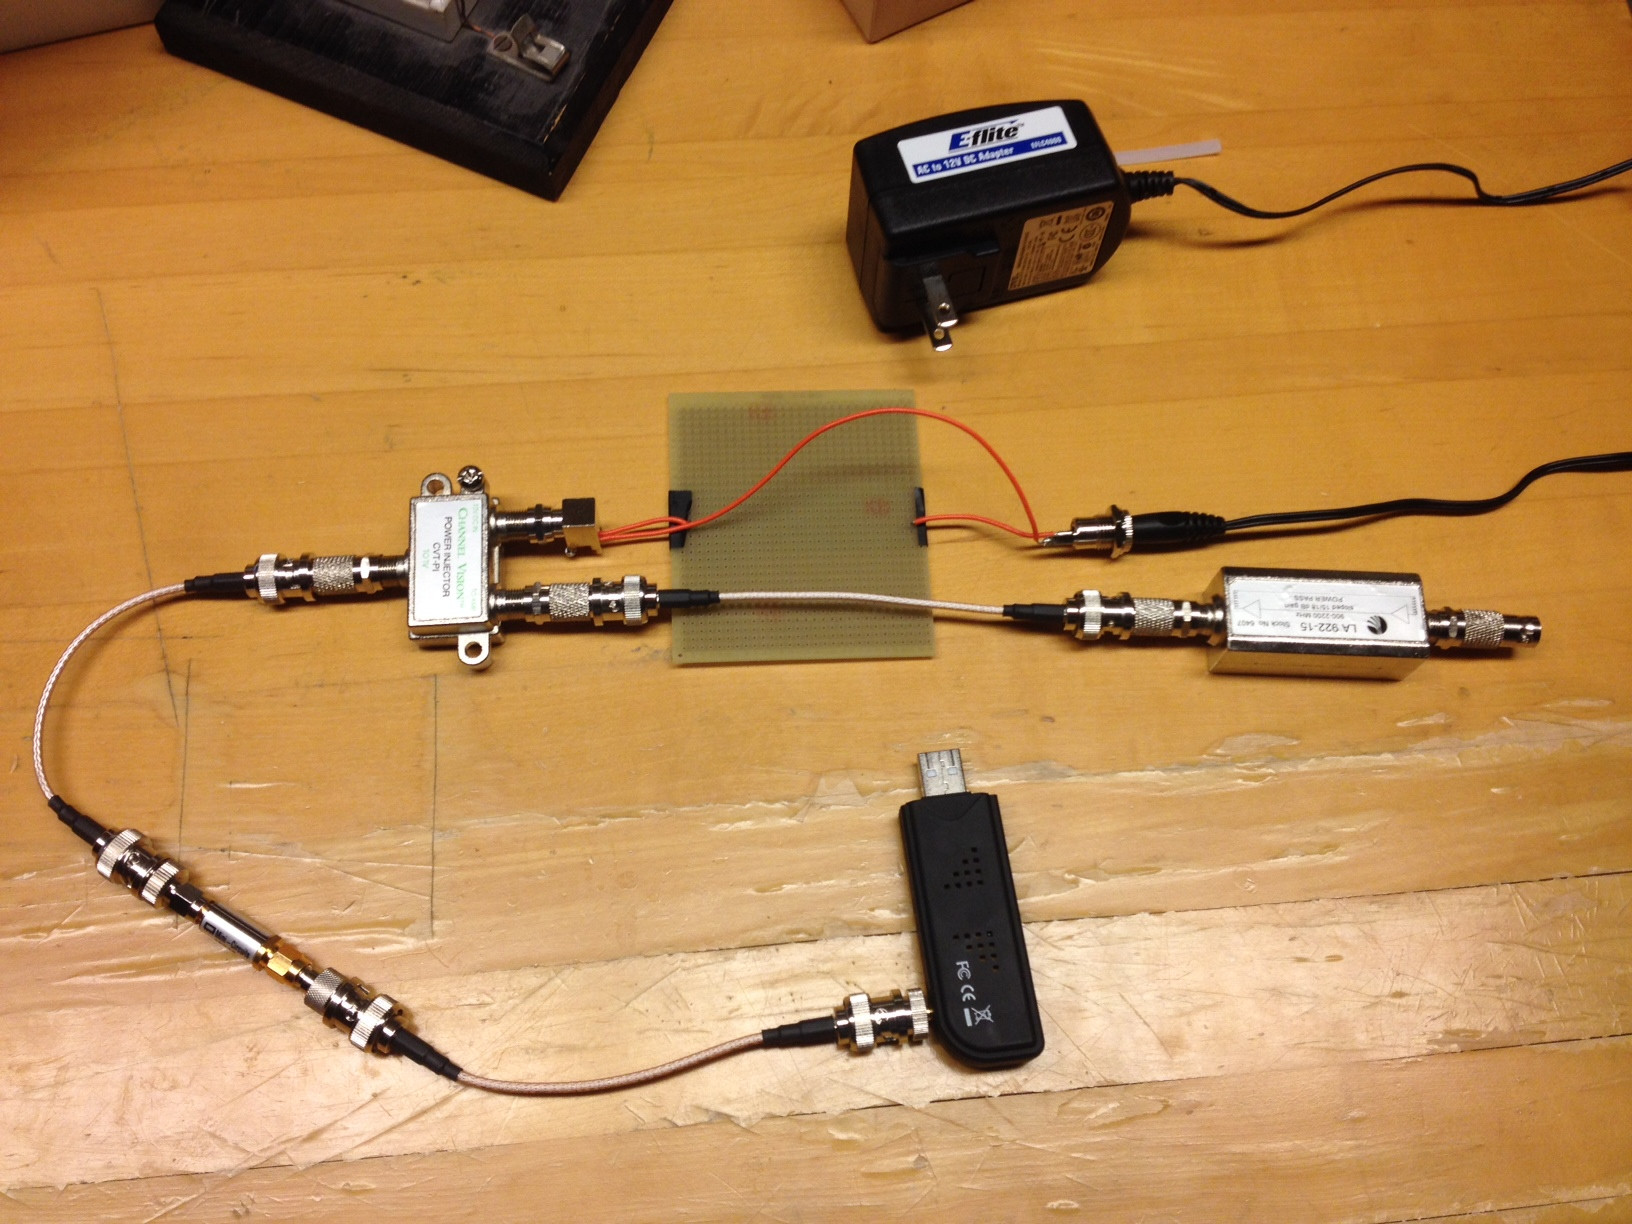
\includegraphics[scale=0.20]{lna/11.jpeg}
\end{center}

%%%%%%%%%%%%%%%%%%%%%%%%%%%%%%%%%%%%%%%%

\subsection{Feed}

\subsubsection{Cutting Styrofoam Rod}
We used a hack saw in a jig to get perfectly straight cuts in the 2.5" Styrofoam rod. 

\begin{center}
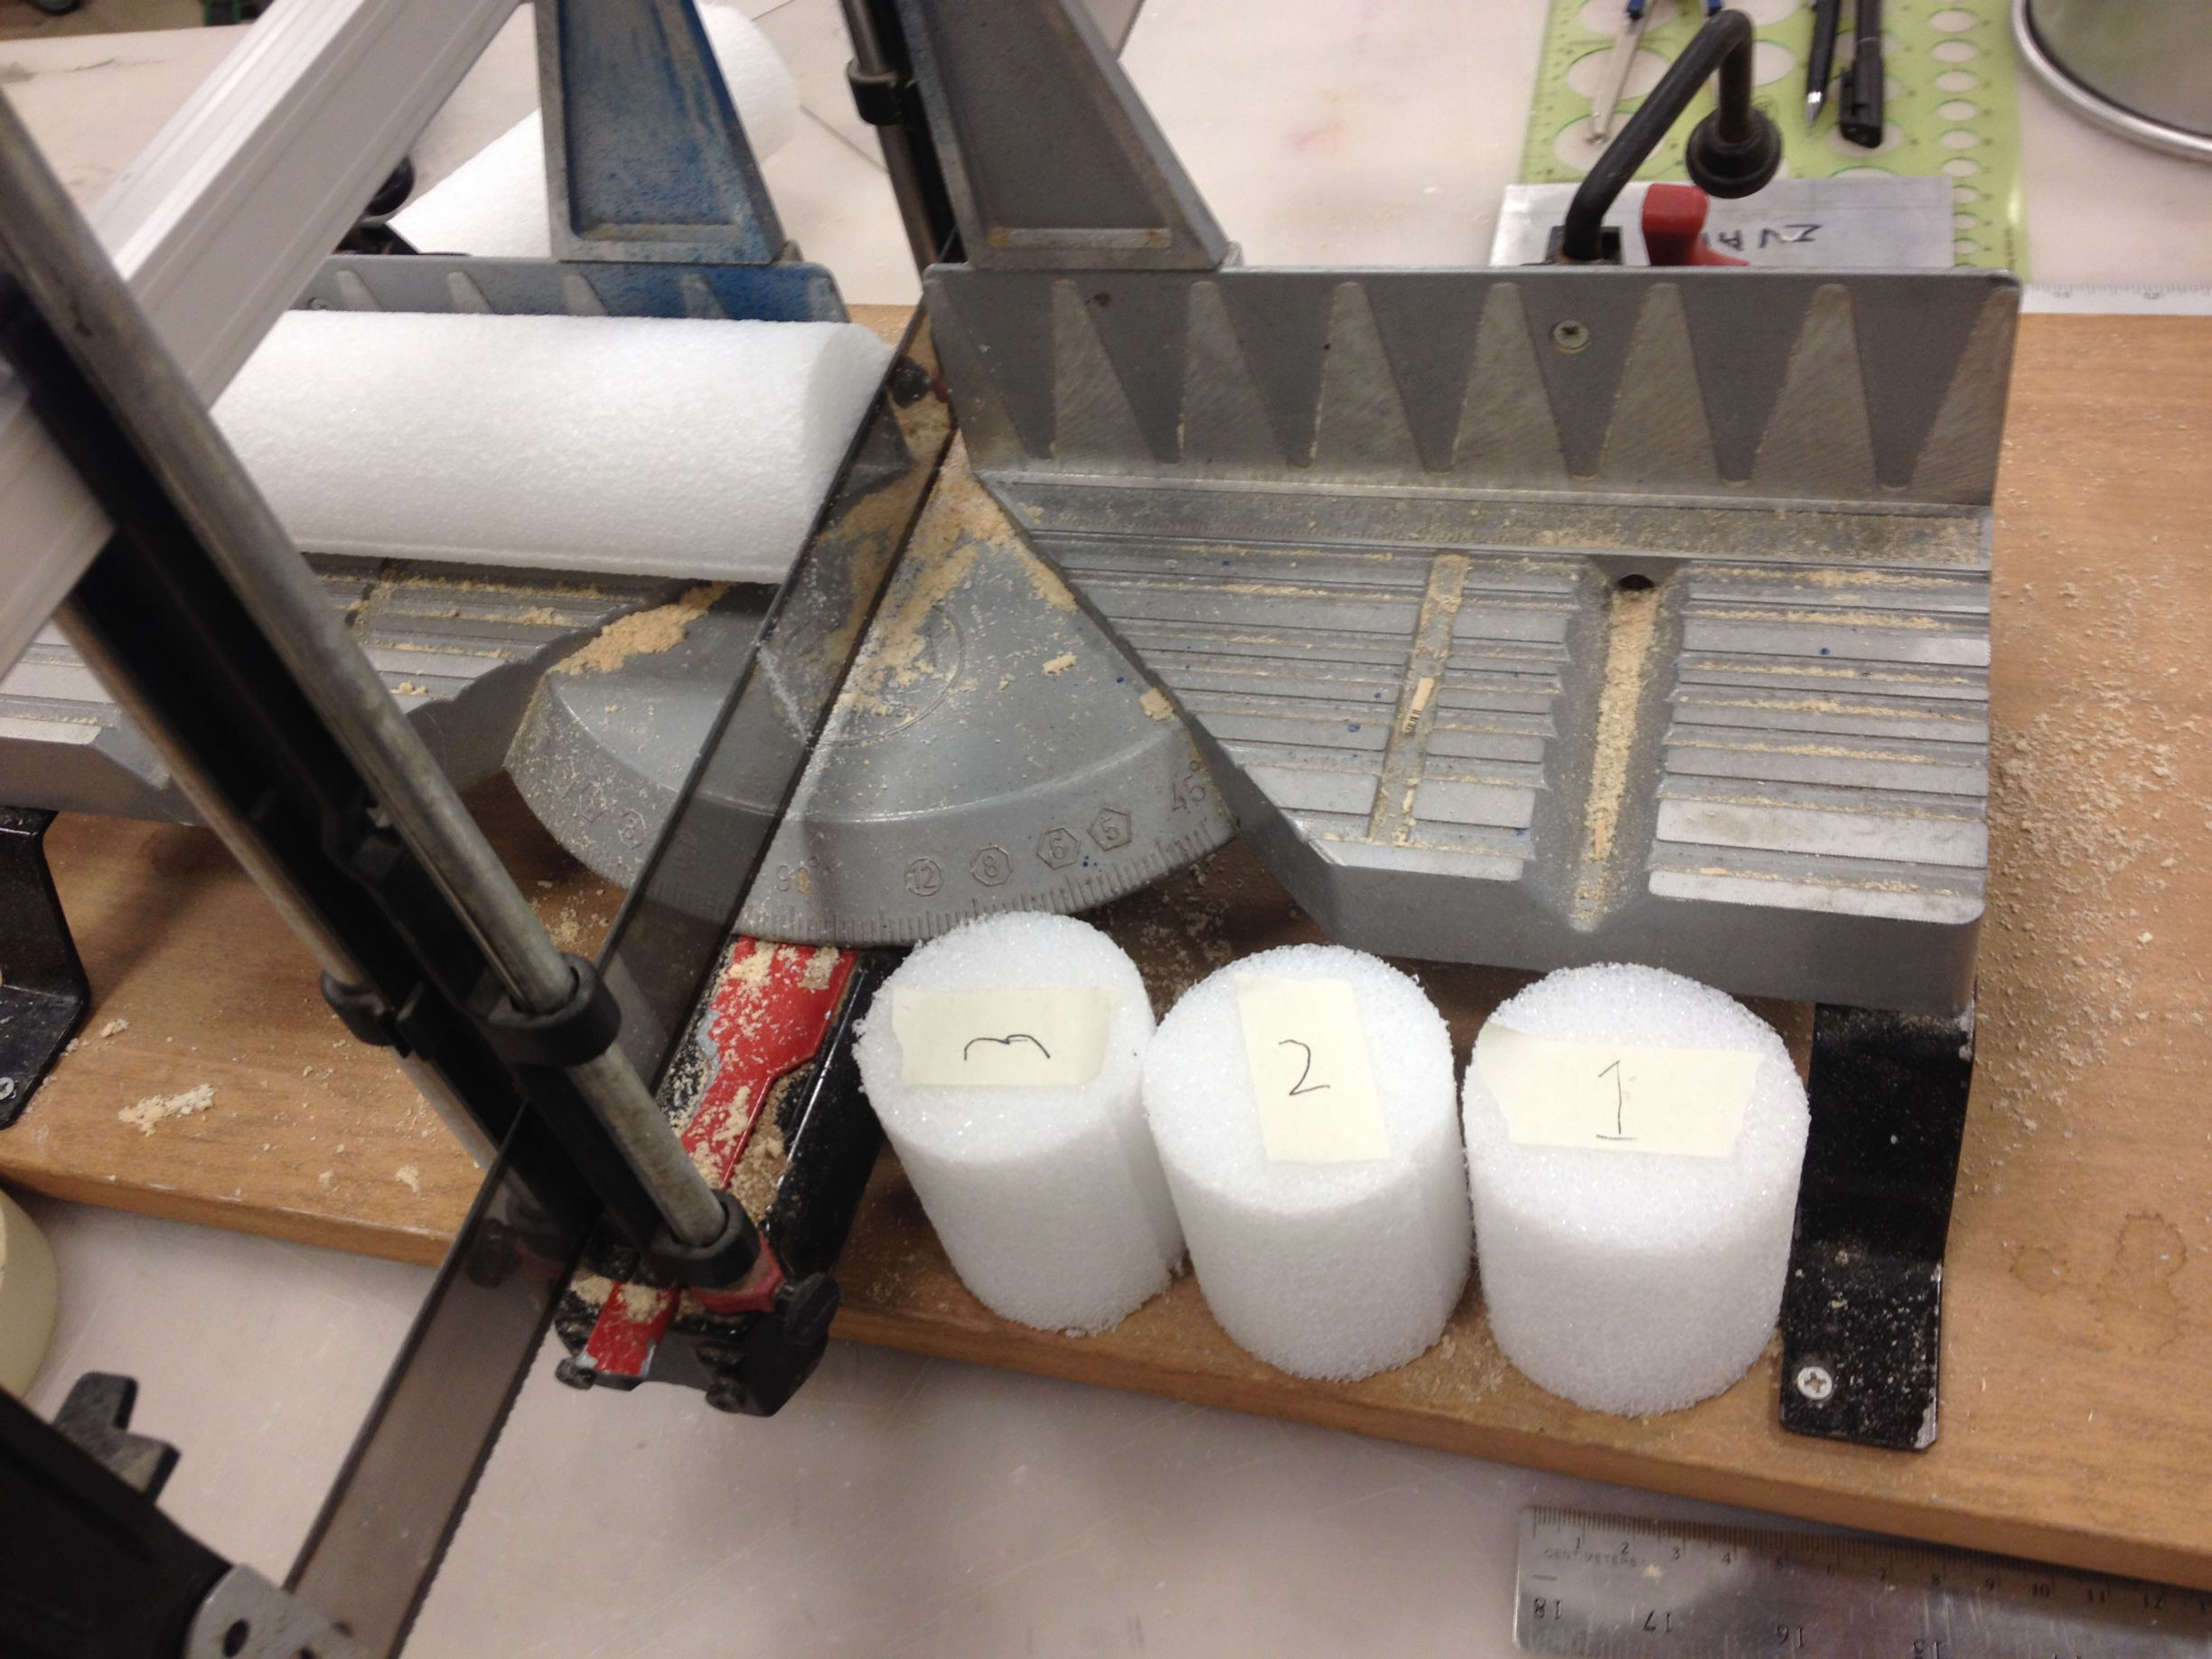
\includegraphics[scale=0.15]{feed/01.jpeg}
\end{center}

The Styrofoam was measured from multiple sides to determine the center. The rod we have ranges from 2 5/16" to 2 1/2" in diameter.

We used a drill press with a 1/4" bit. The Styrofoam was held by a vice on the drilling table. (The Styrofoam is a bit messy so we put down a rag under the vice) 

\begin{center}
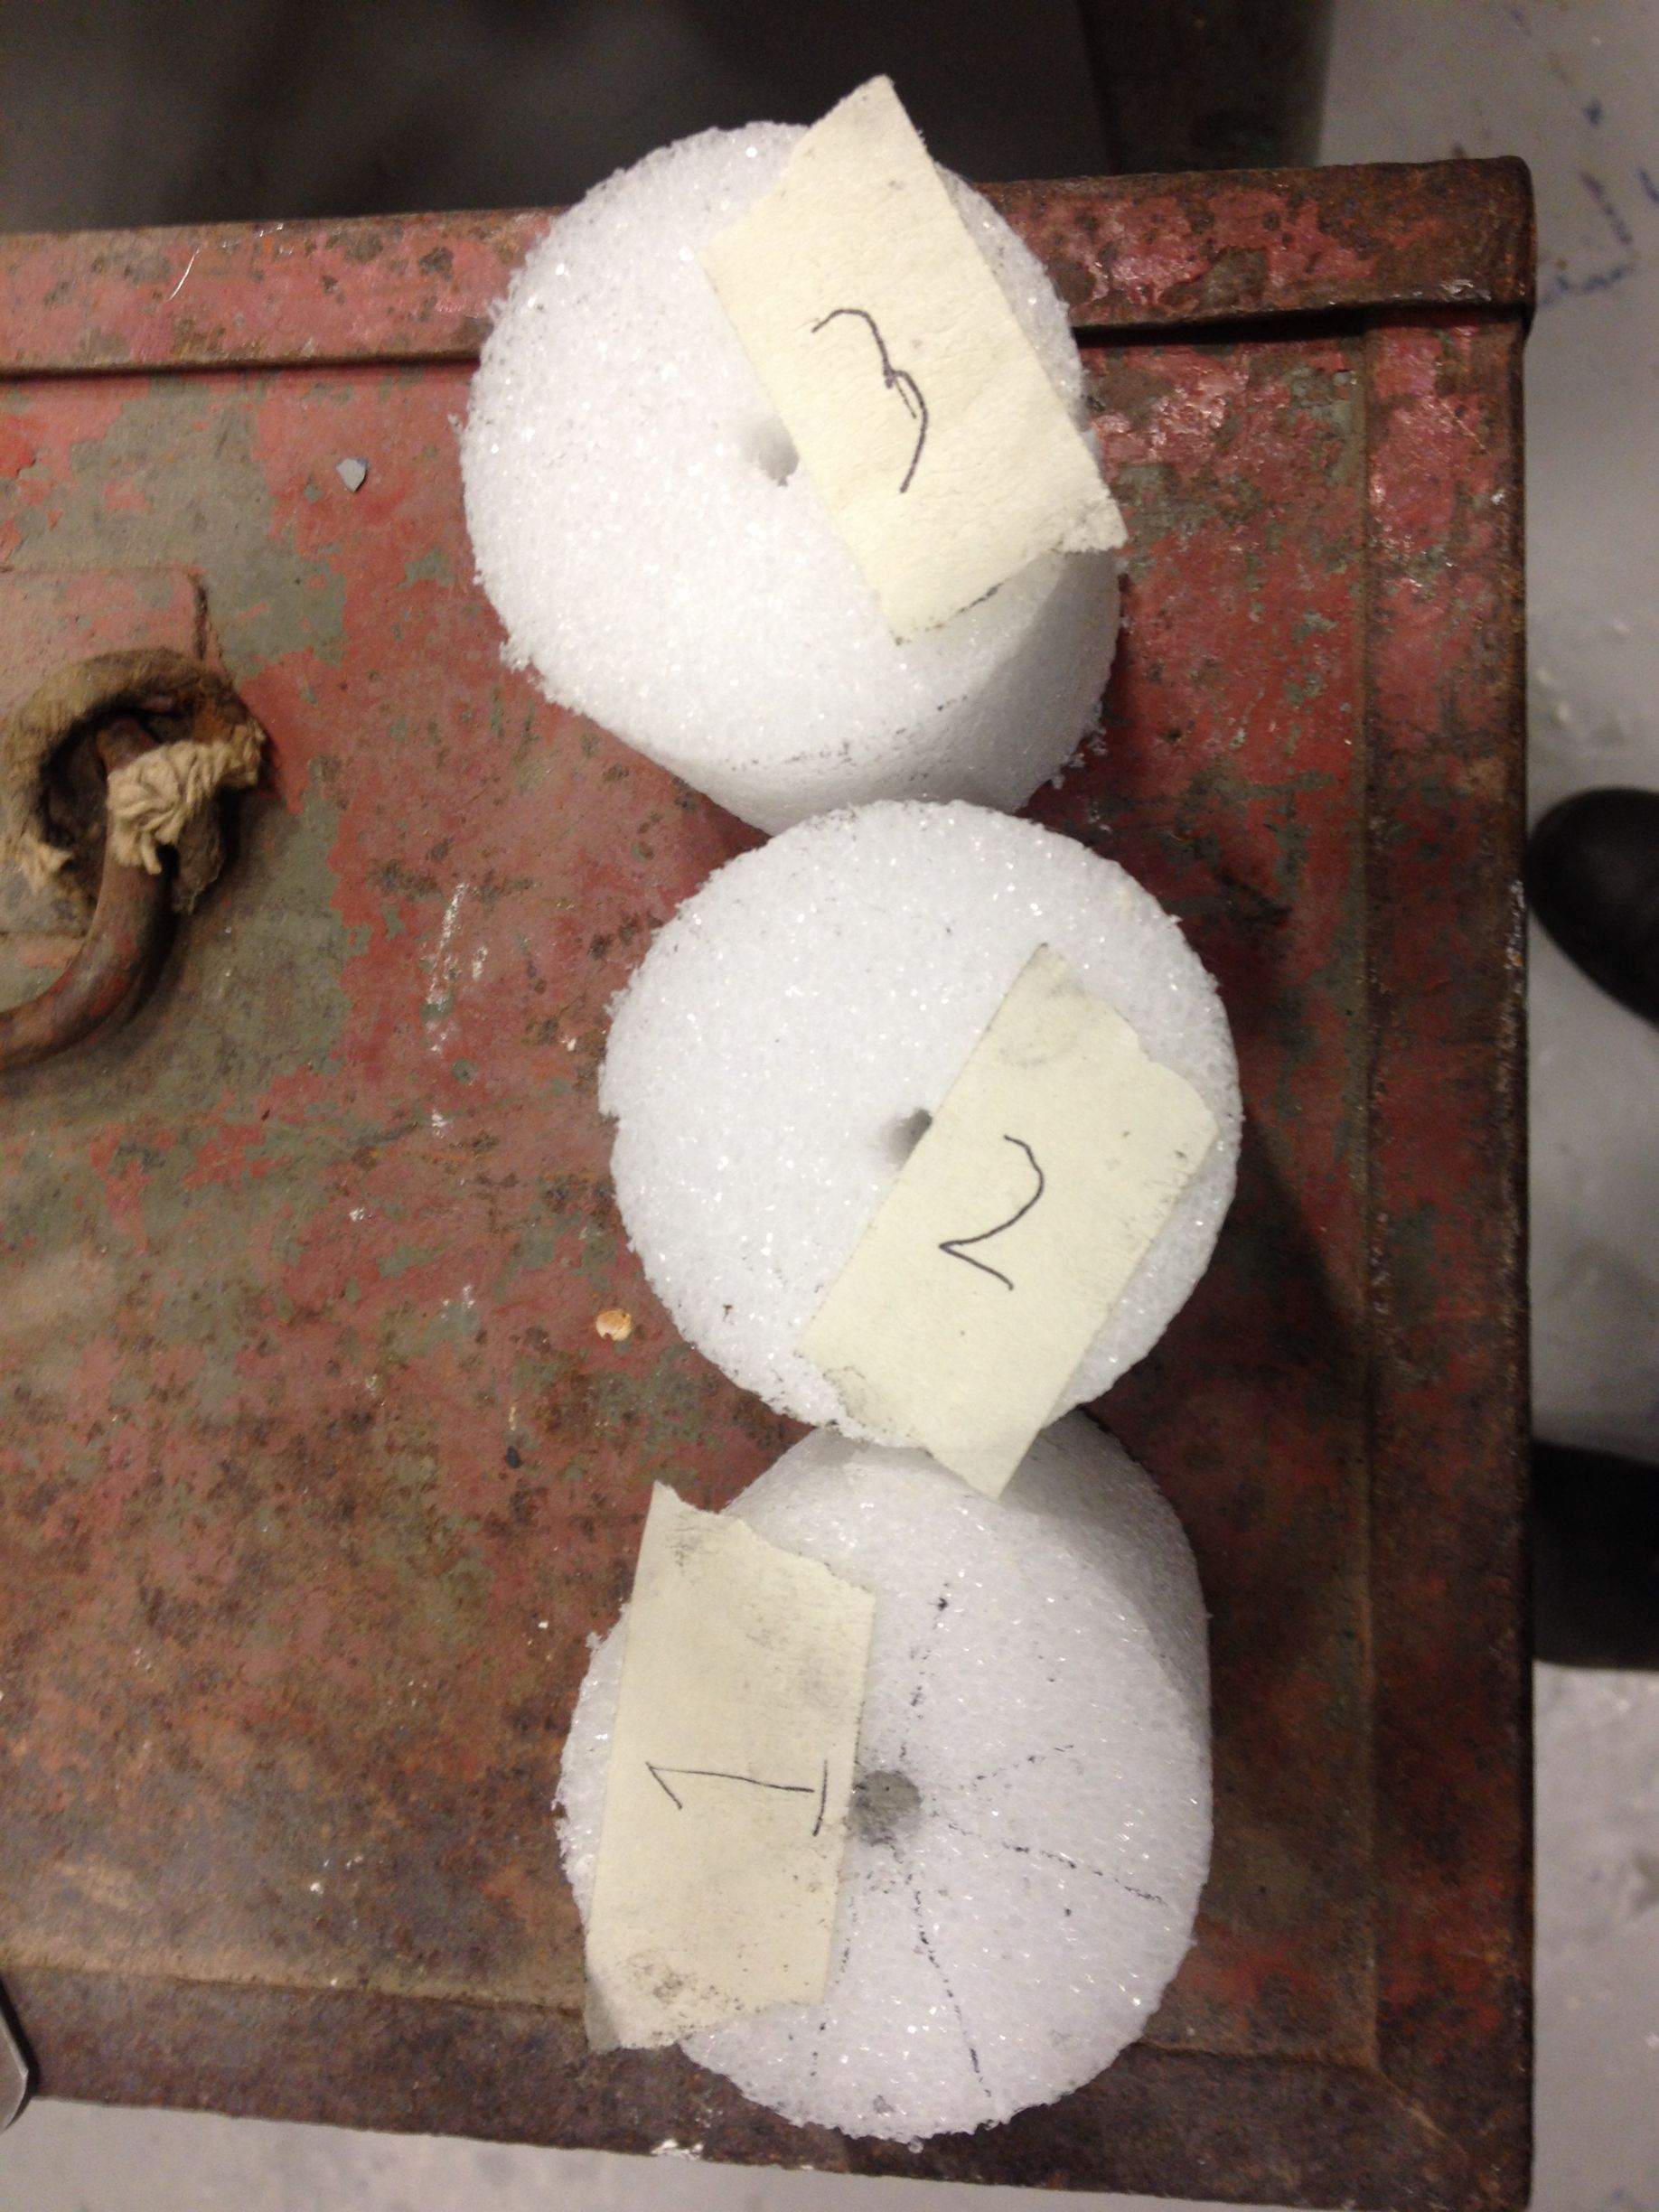
\includegraphics[scale=0.09]{feed/02.jpeg}
\end{center}

Note: we made three rods to provide room for error in the application and soldering of the copper tape later.

\subsubsection{Drilling Aluminum LNA Base Plate}

We put the plate in a vice which we secured on the drill press table with some heavy steel blocks.

\begin{center}
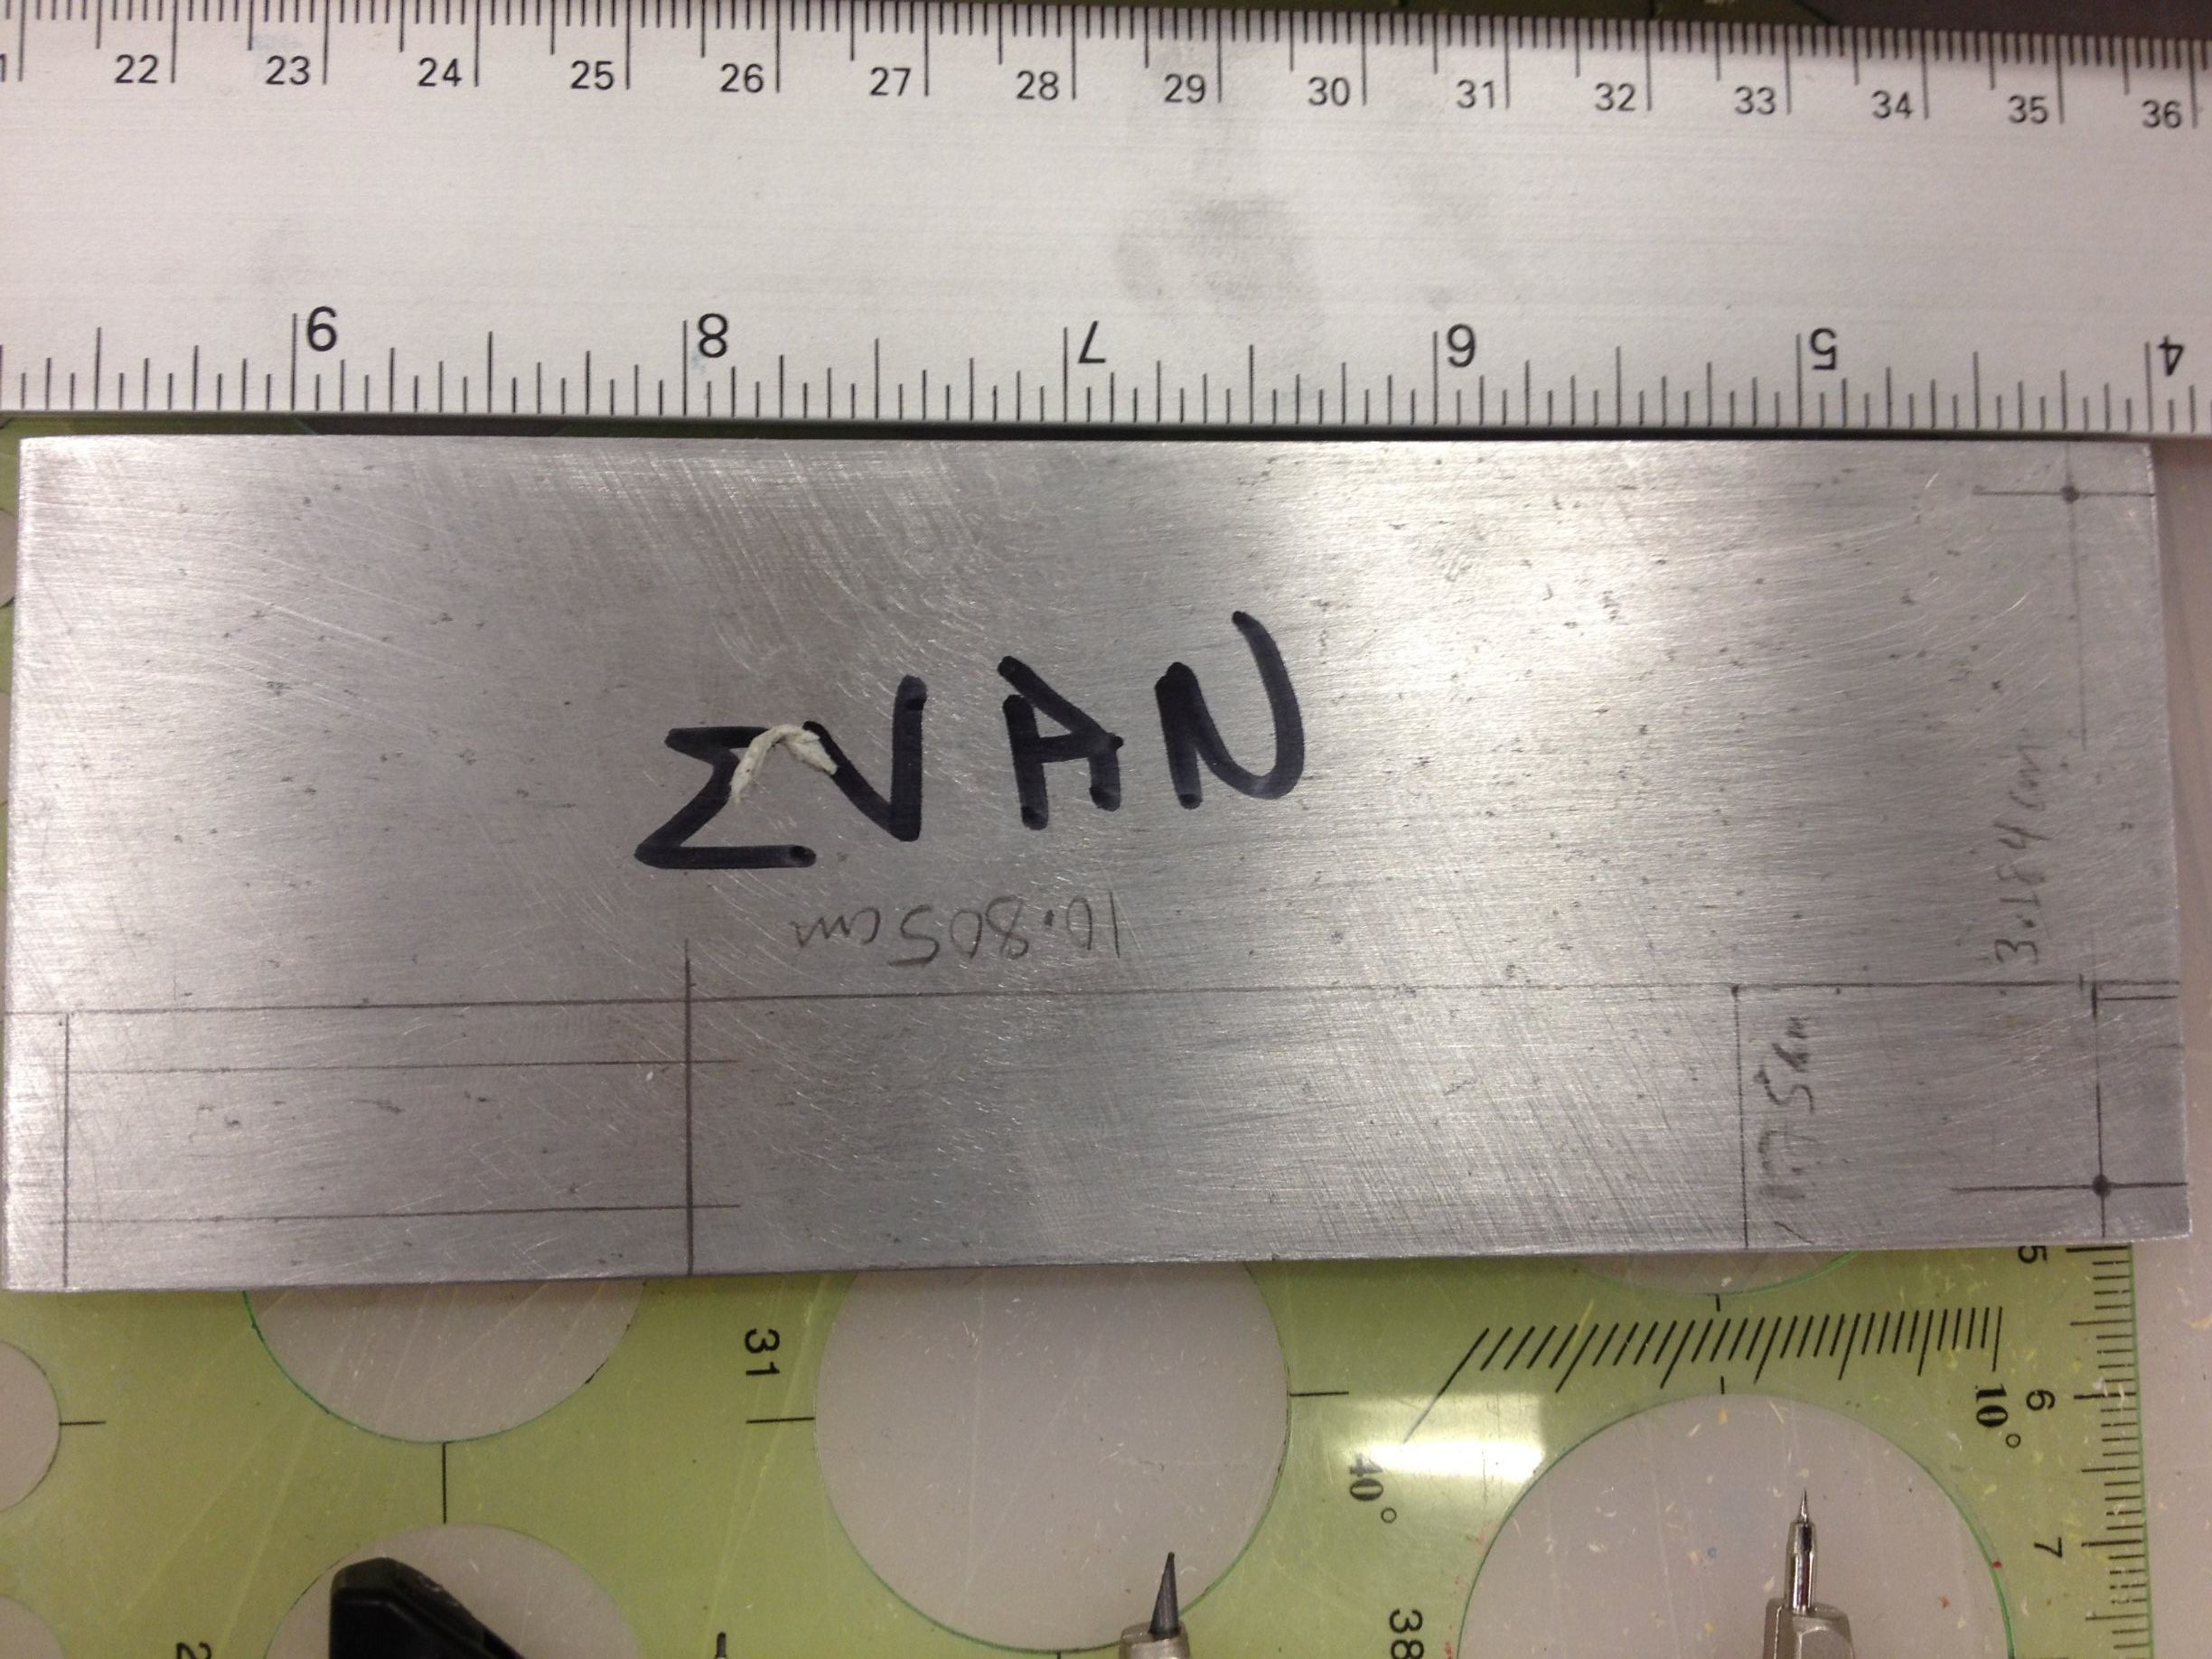
\includegraphics[scale=0.12]{feed/03.jpeg}
\end{center}

\subsubsection{Drilling Aluminum Cake Pan}

We made the measurements of the cake pan working out from the center which we found by transecting the circle and then making perpendicular rays from the center of each line cutting across the arc. This proved to be adequately precise. 

\begin{center}
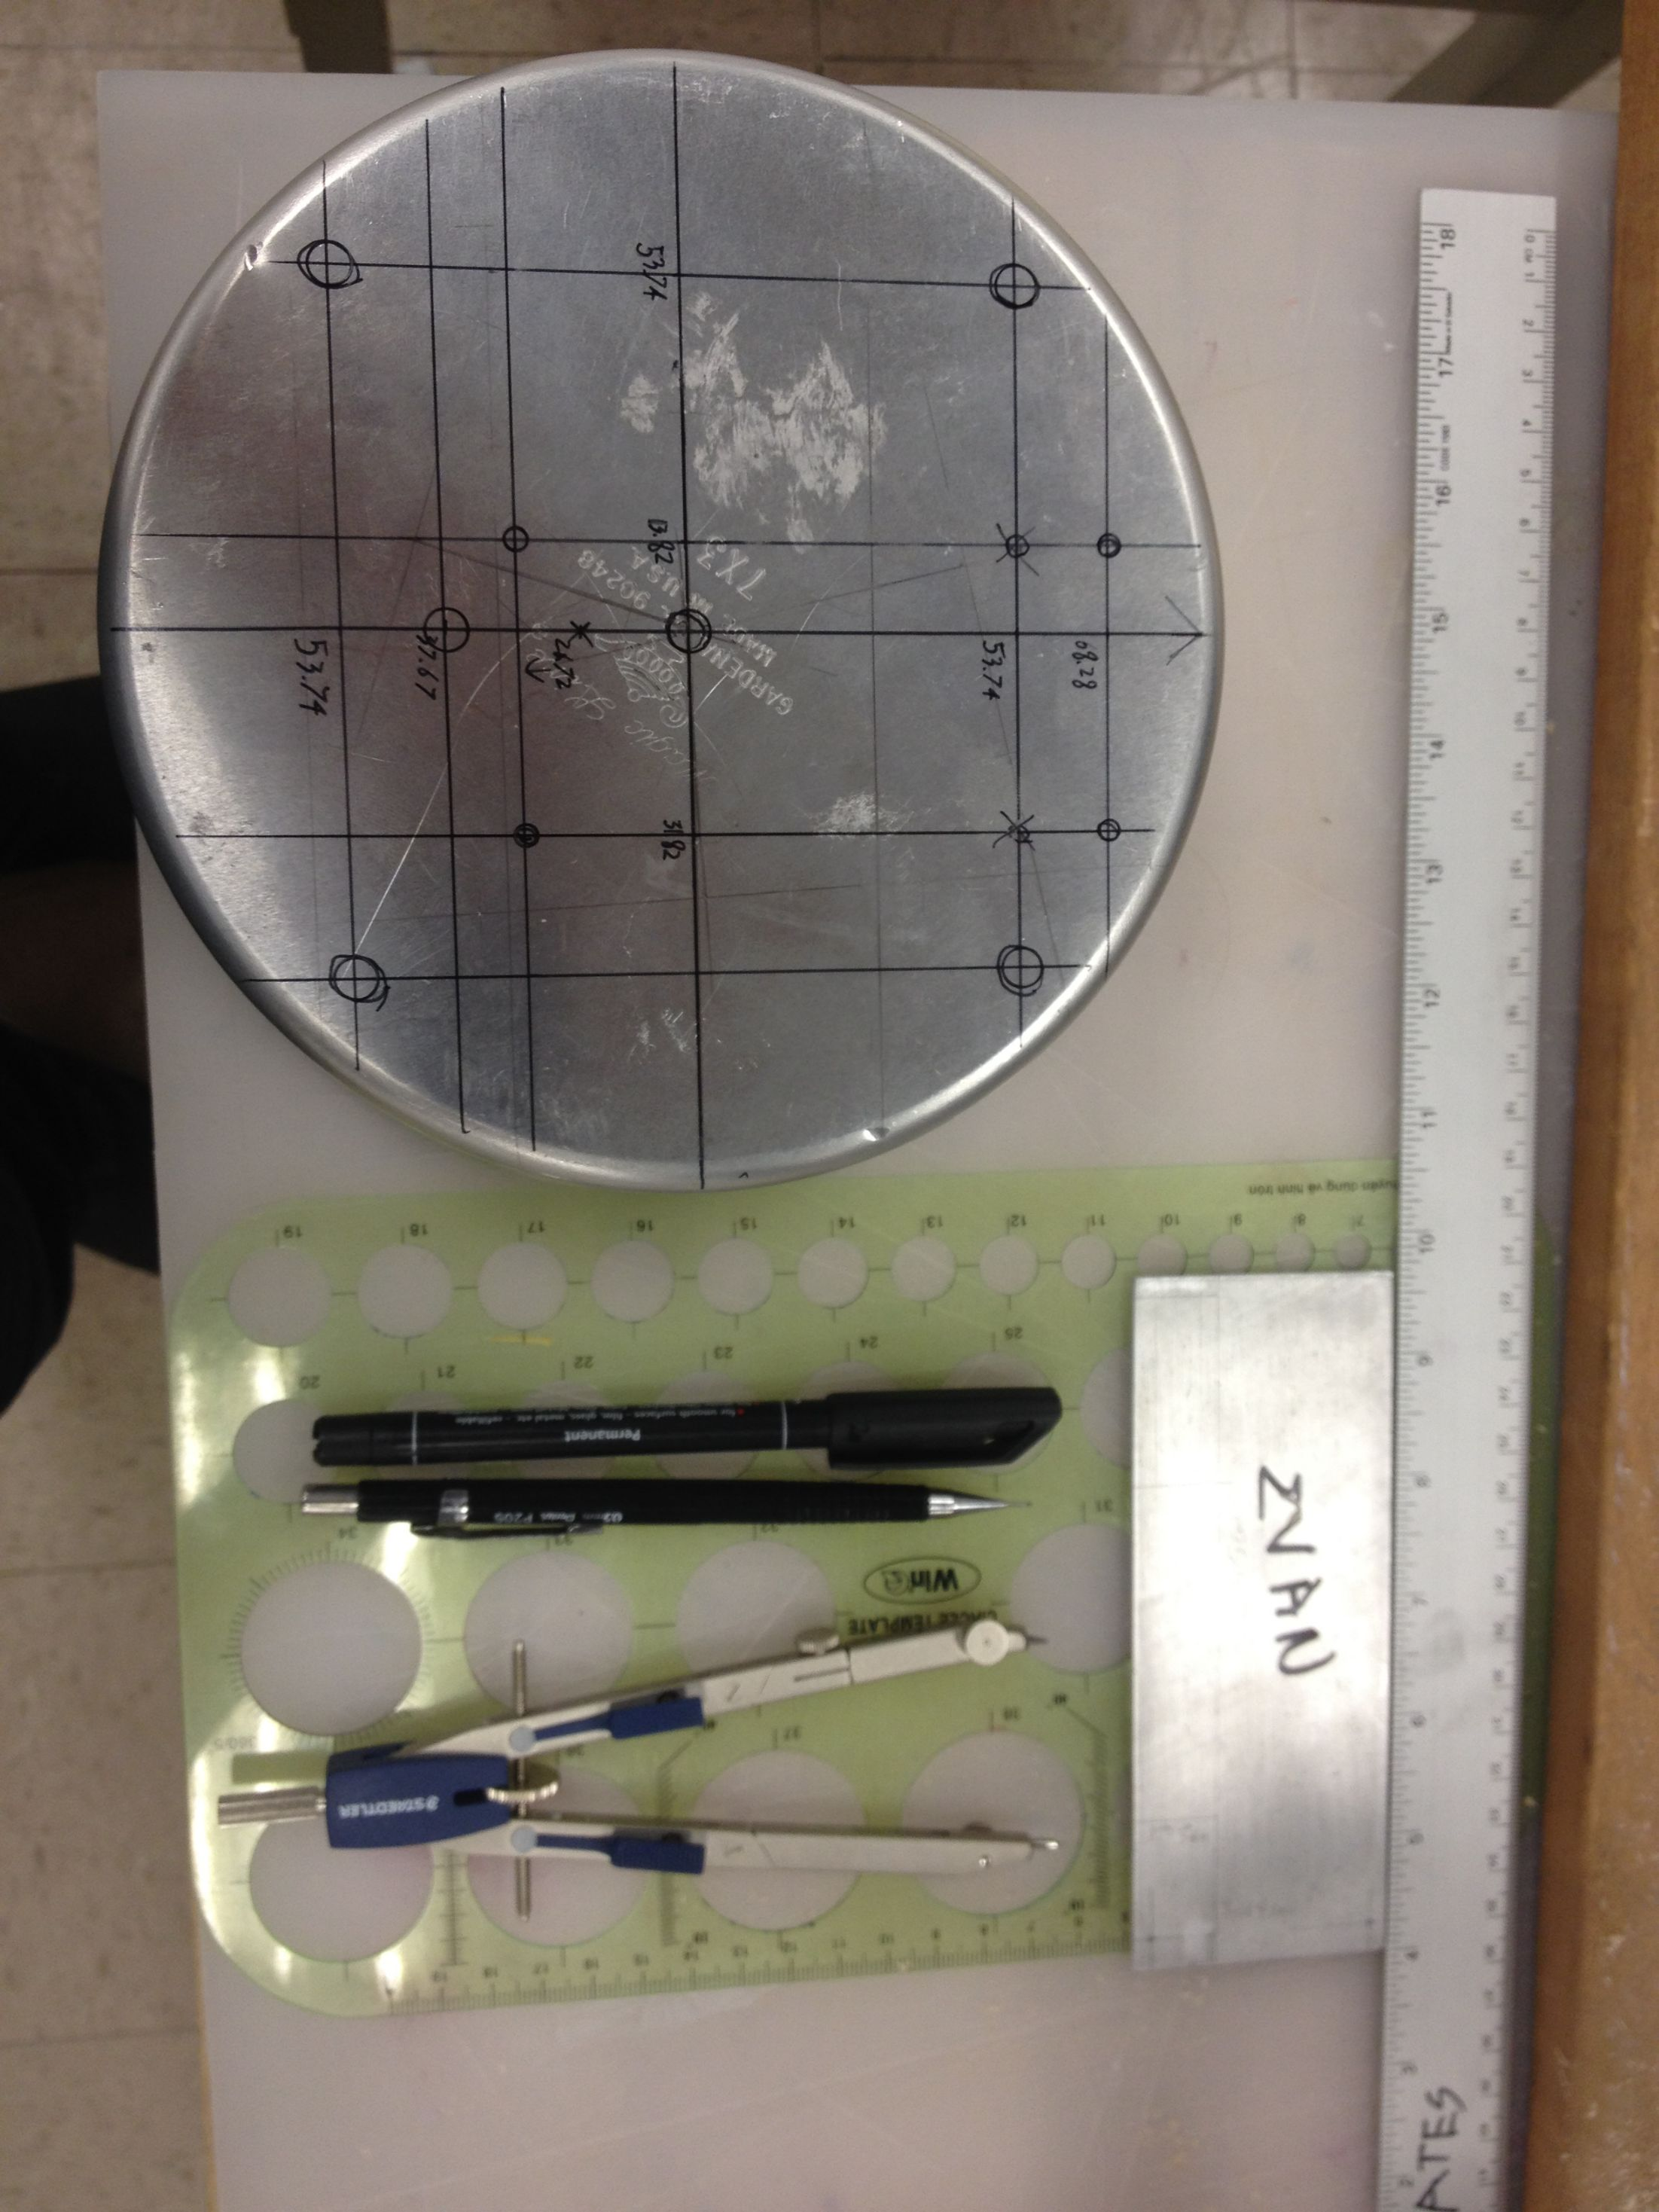
\includegraphics[scale=0.11]{feed/04.jpeg}
\end{center}

The cake pan was more of a challenge to drill than the base plate as it was tricky to secure to the drill press table so we could make accurate holes. We ended up putting a 4" piece of angle iron on the pan and then clamping that down to the edges of the table. 

\begin{center}
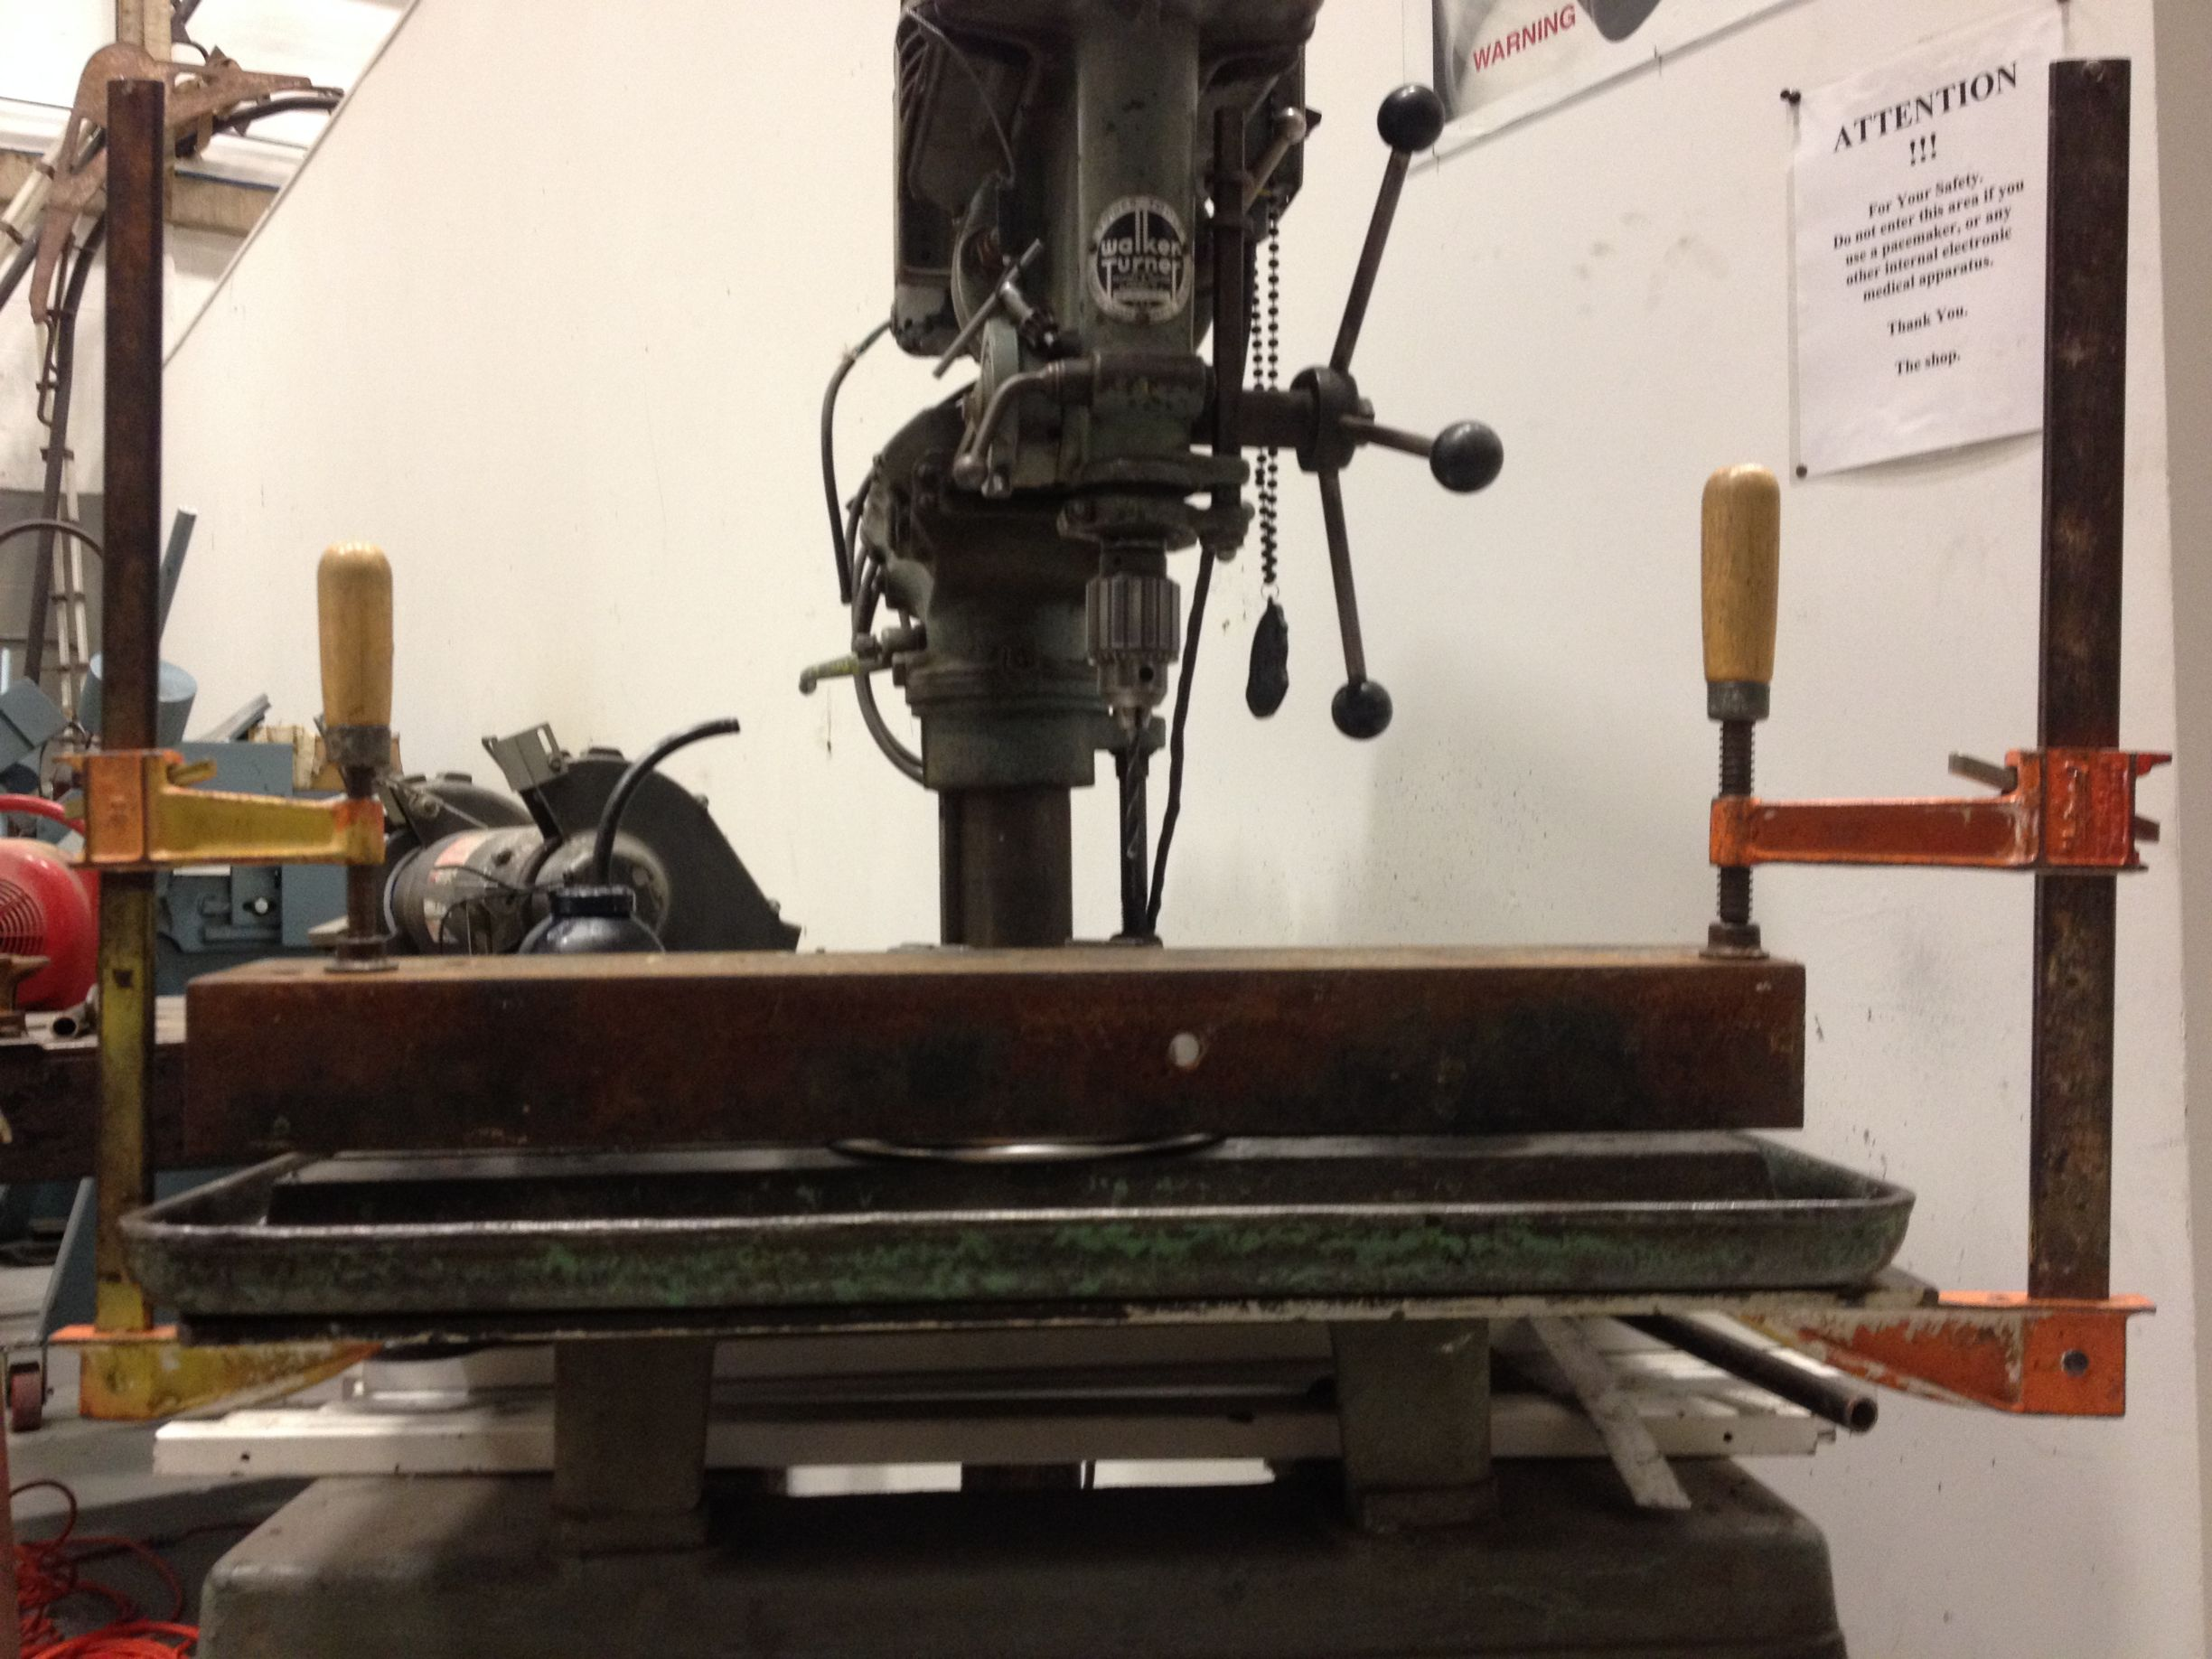
\includegraphics[scale=0.15]{feed/05.jpeg}
\end{center}

Finished drilling

\begin{center}
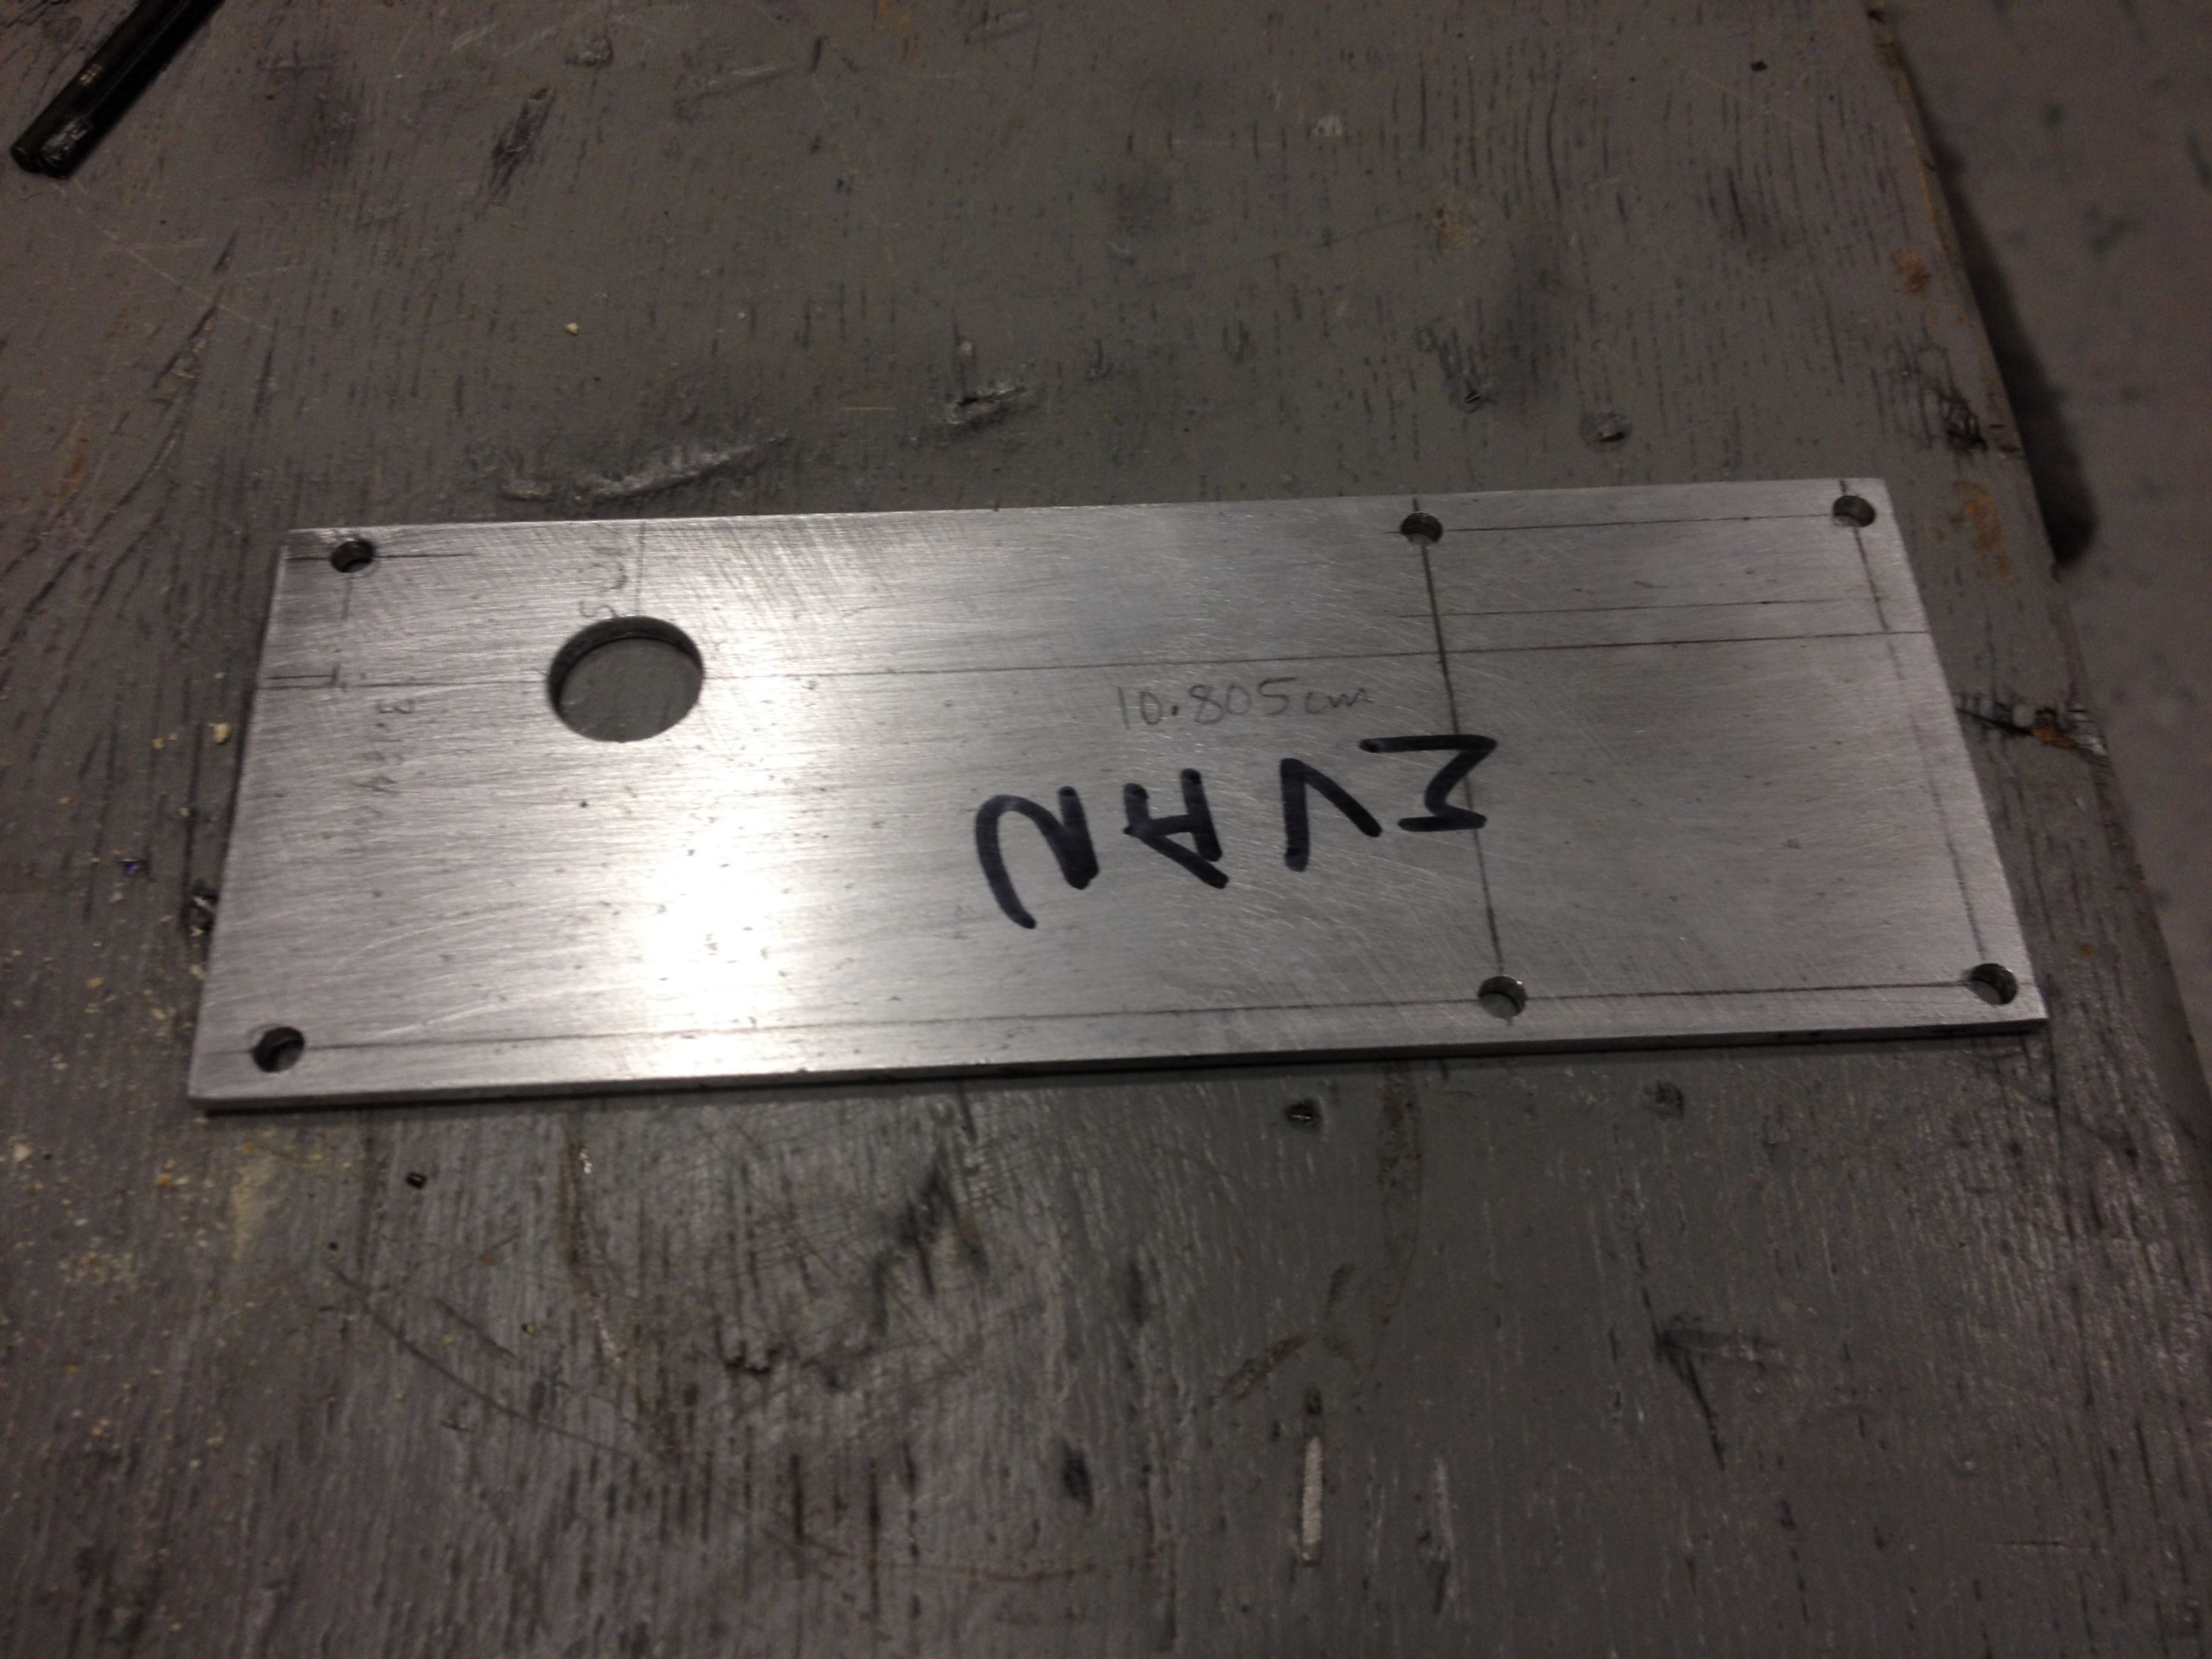
\includegraphics[scale=0.10]{feed/06.jpeg}
\end{center}

\begin{center}
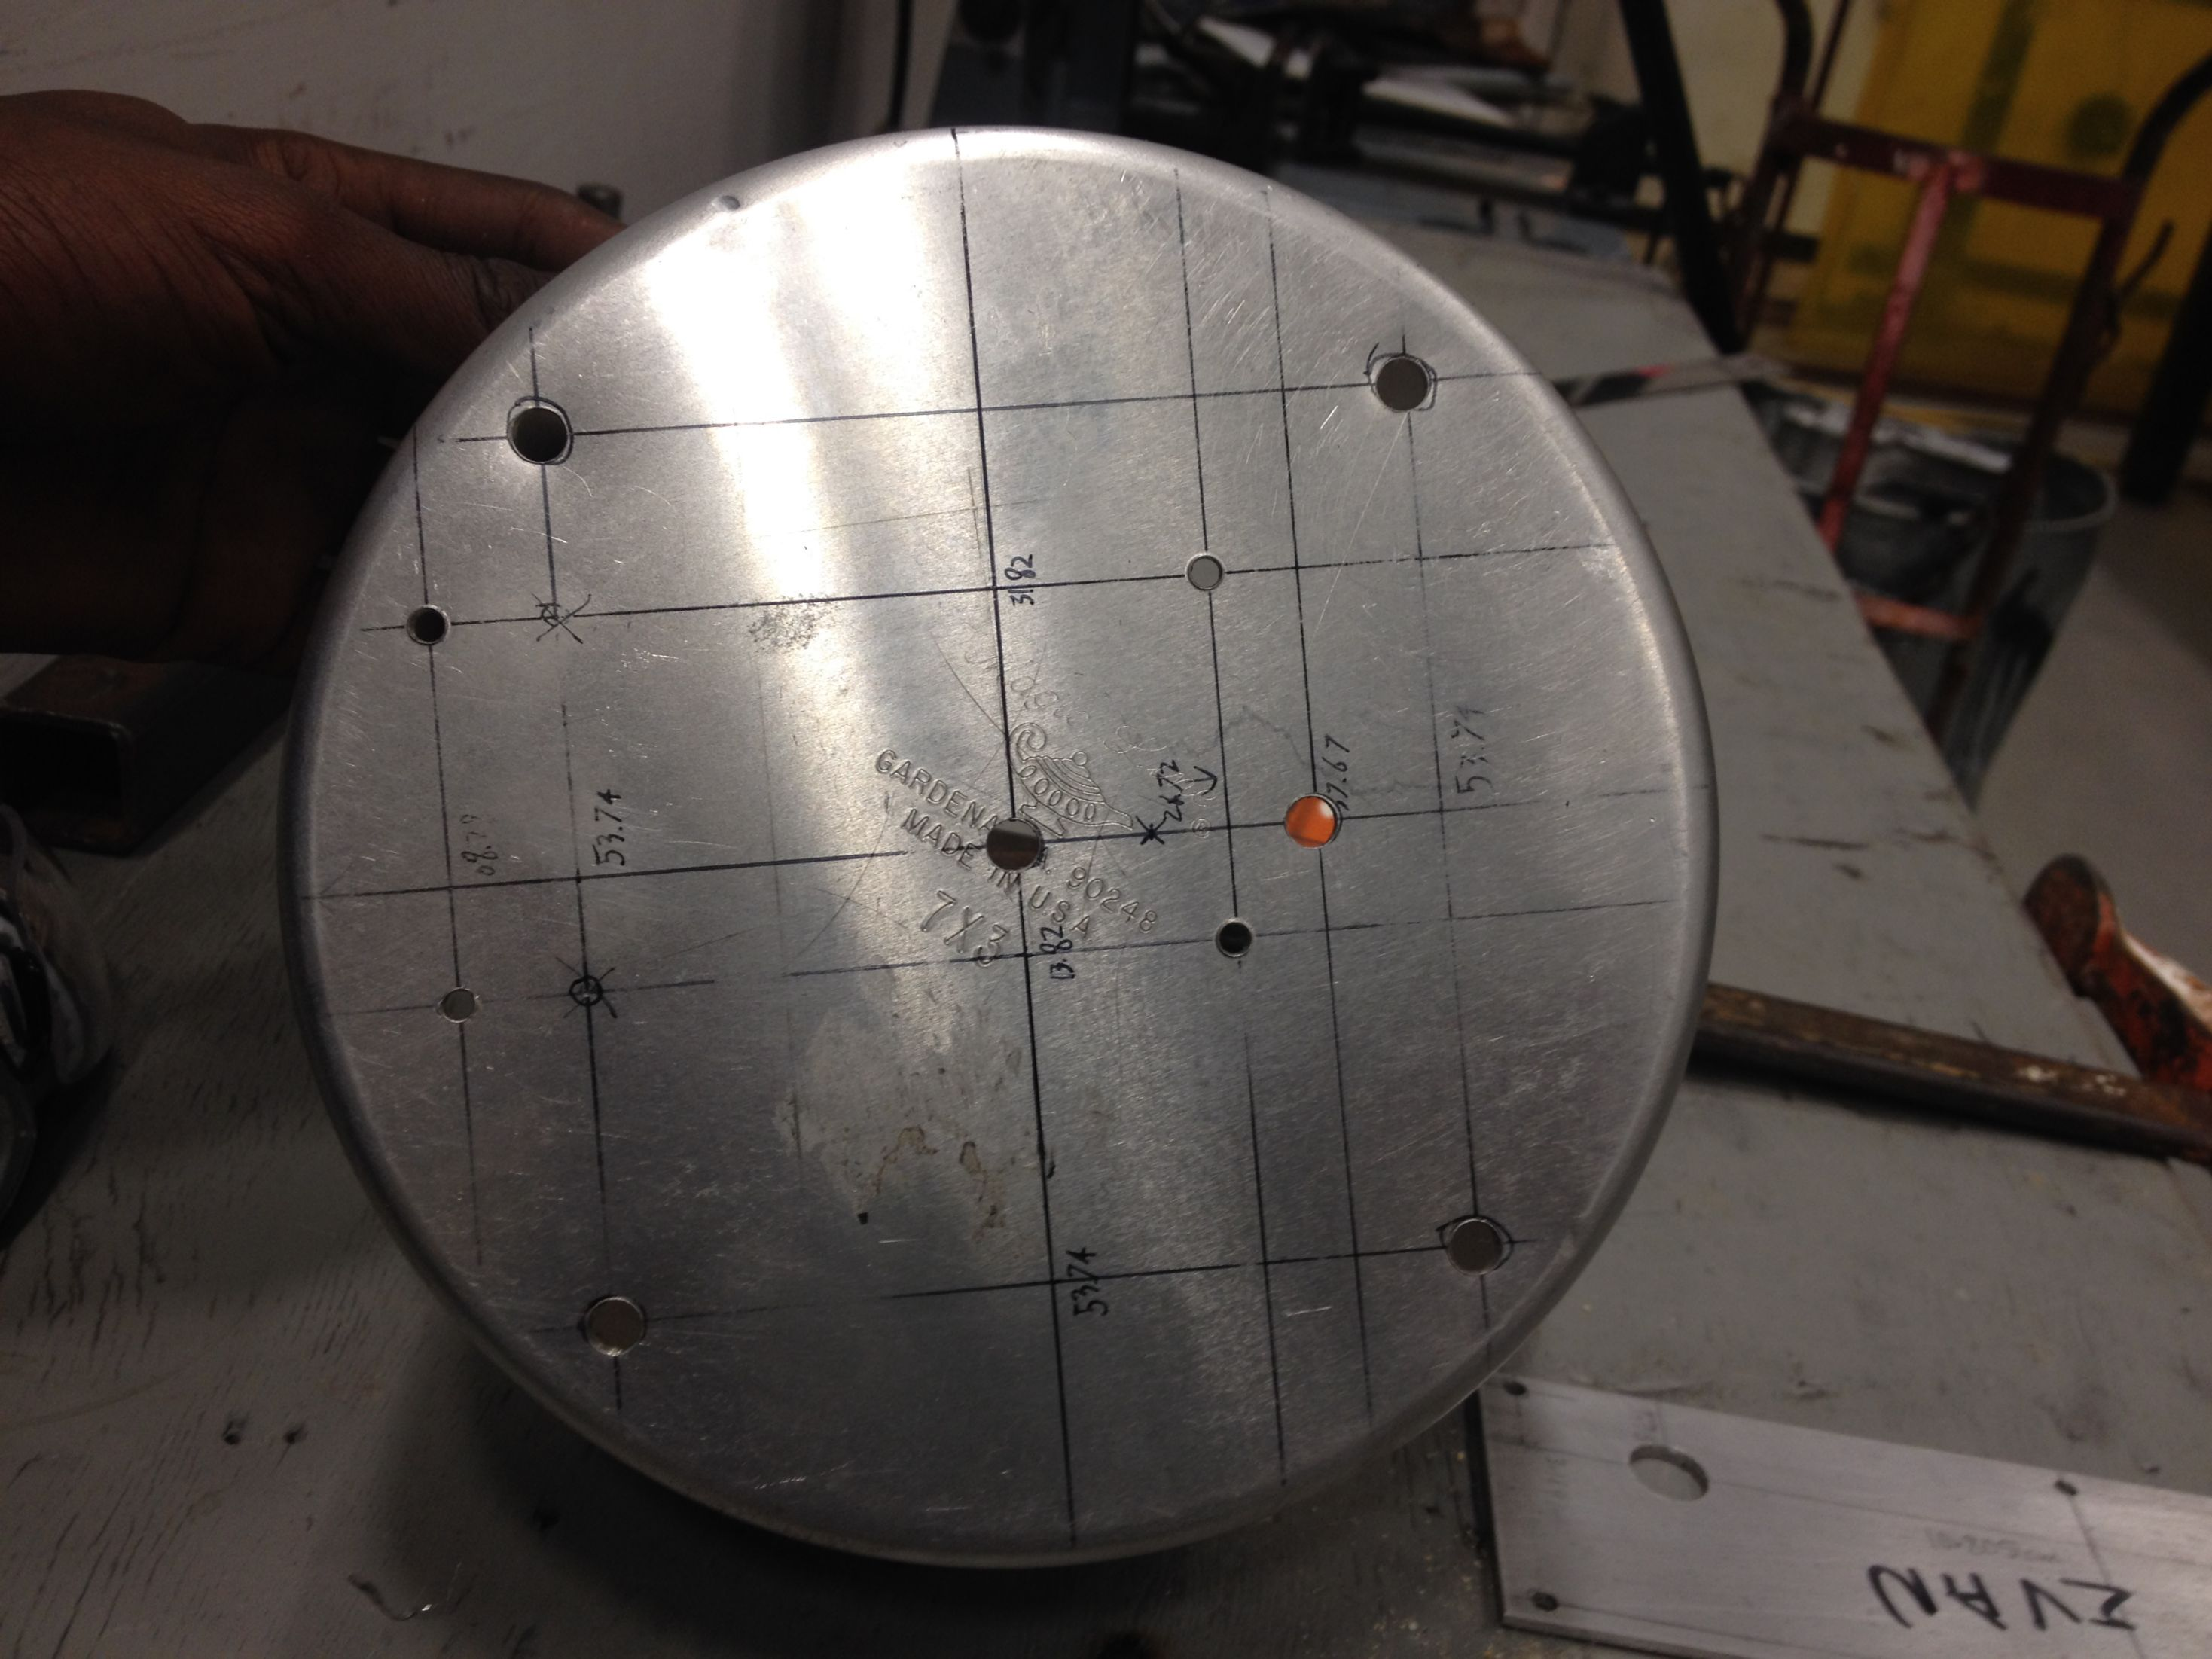
\includegraphics[scale=0.11]{feed/07.jpeg}
\end{center}

\subsubsection{Minor concerns}
The drilling instructions are precise to a 100th of a millimeter. We did the drilling with a drill press, not a CNC machine, so I would say our precision was closer to a 10th of a millimeter.

Also, the cake pan is really not a precisely made object, it is certainly not as precise as the schematics given by MIT. I think that indicates that our slight reduction in precision will be fine.

The cake pan is made of what seems to be a softer aluminum than the LNA base plate. This made the metal not cut cleanly on the inside of the pan (the bit went through the outside first). The holes are the correct dimensions but there is some extra material around the holes. I have tried to clean it up with an x-acto knife and been relatively successful. I think the metal is so soft that these small bits of extra material will be squished when we insert the hardware, making their effect negligible. 

\begin{center}
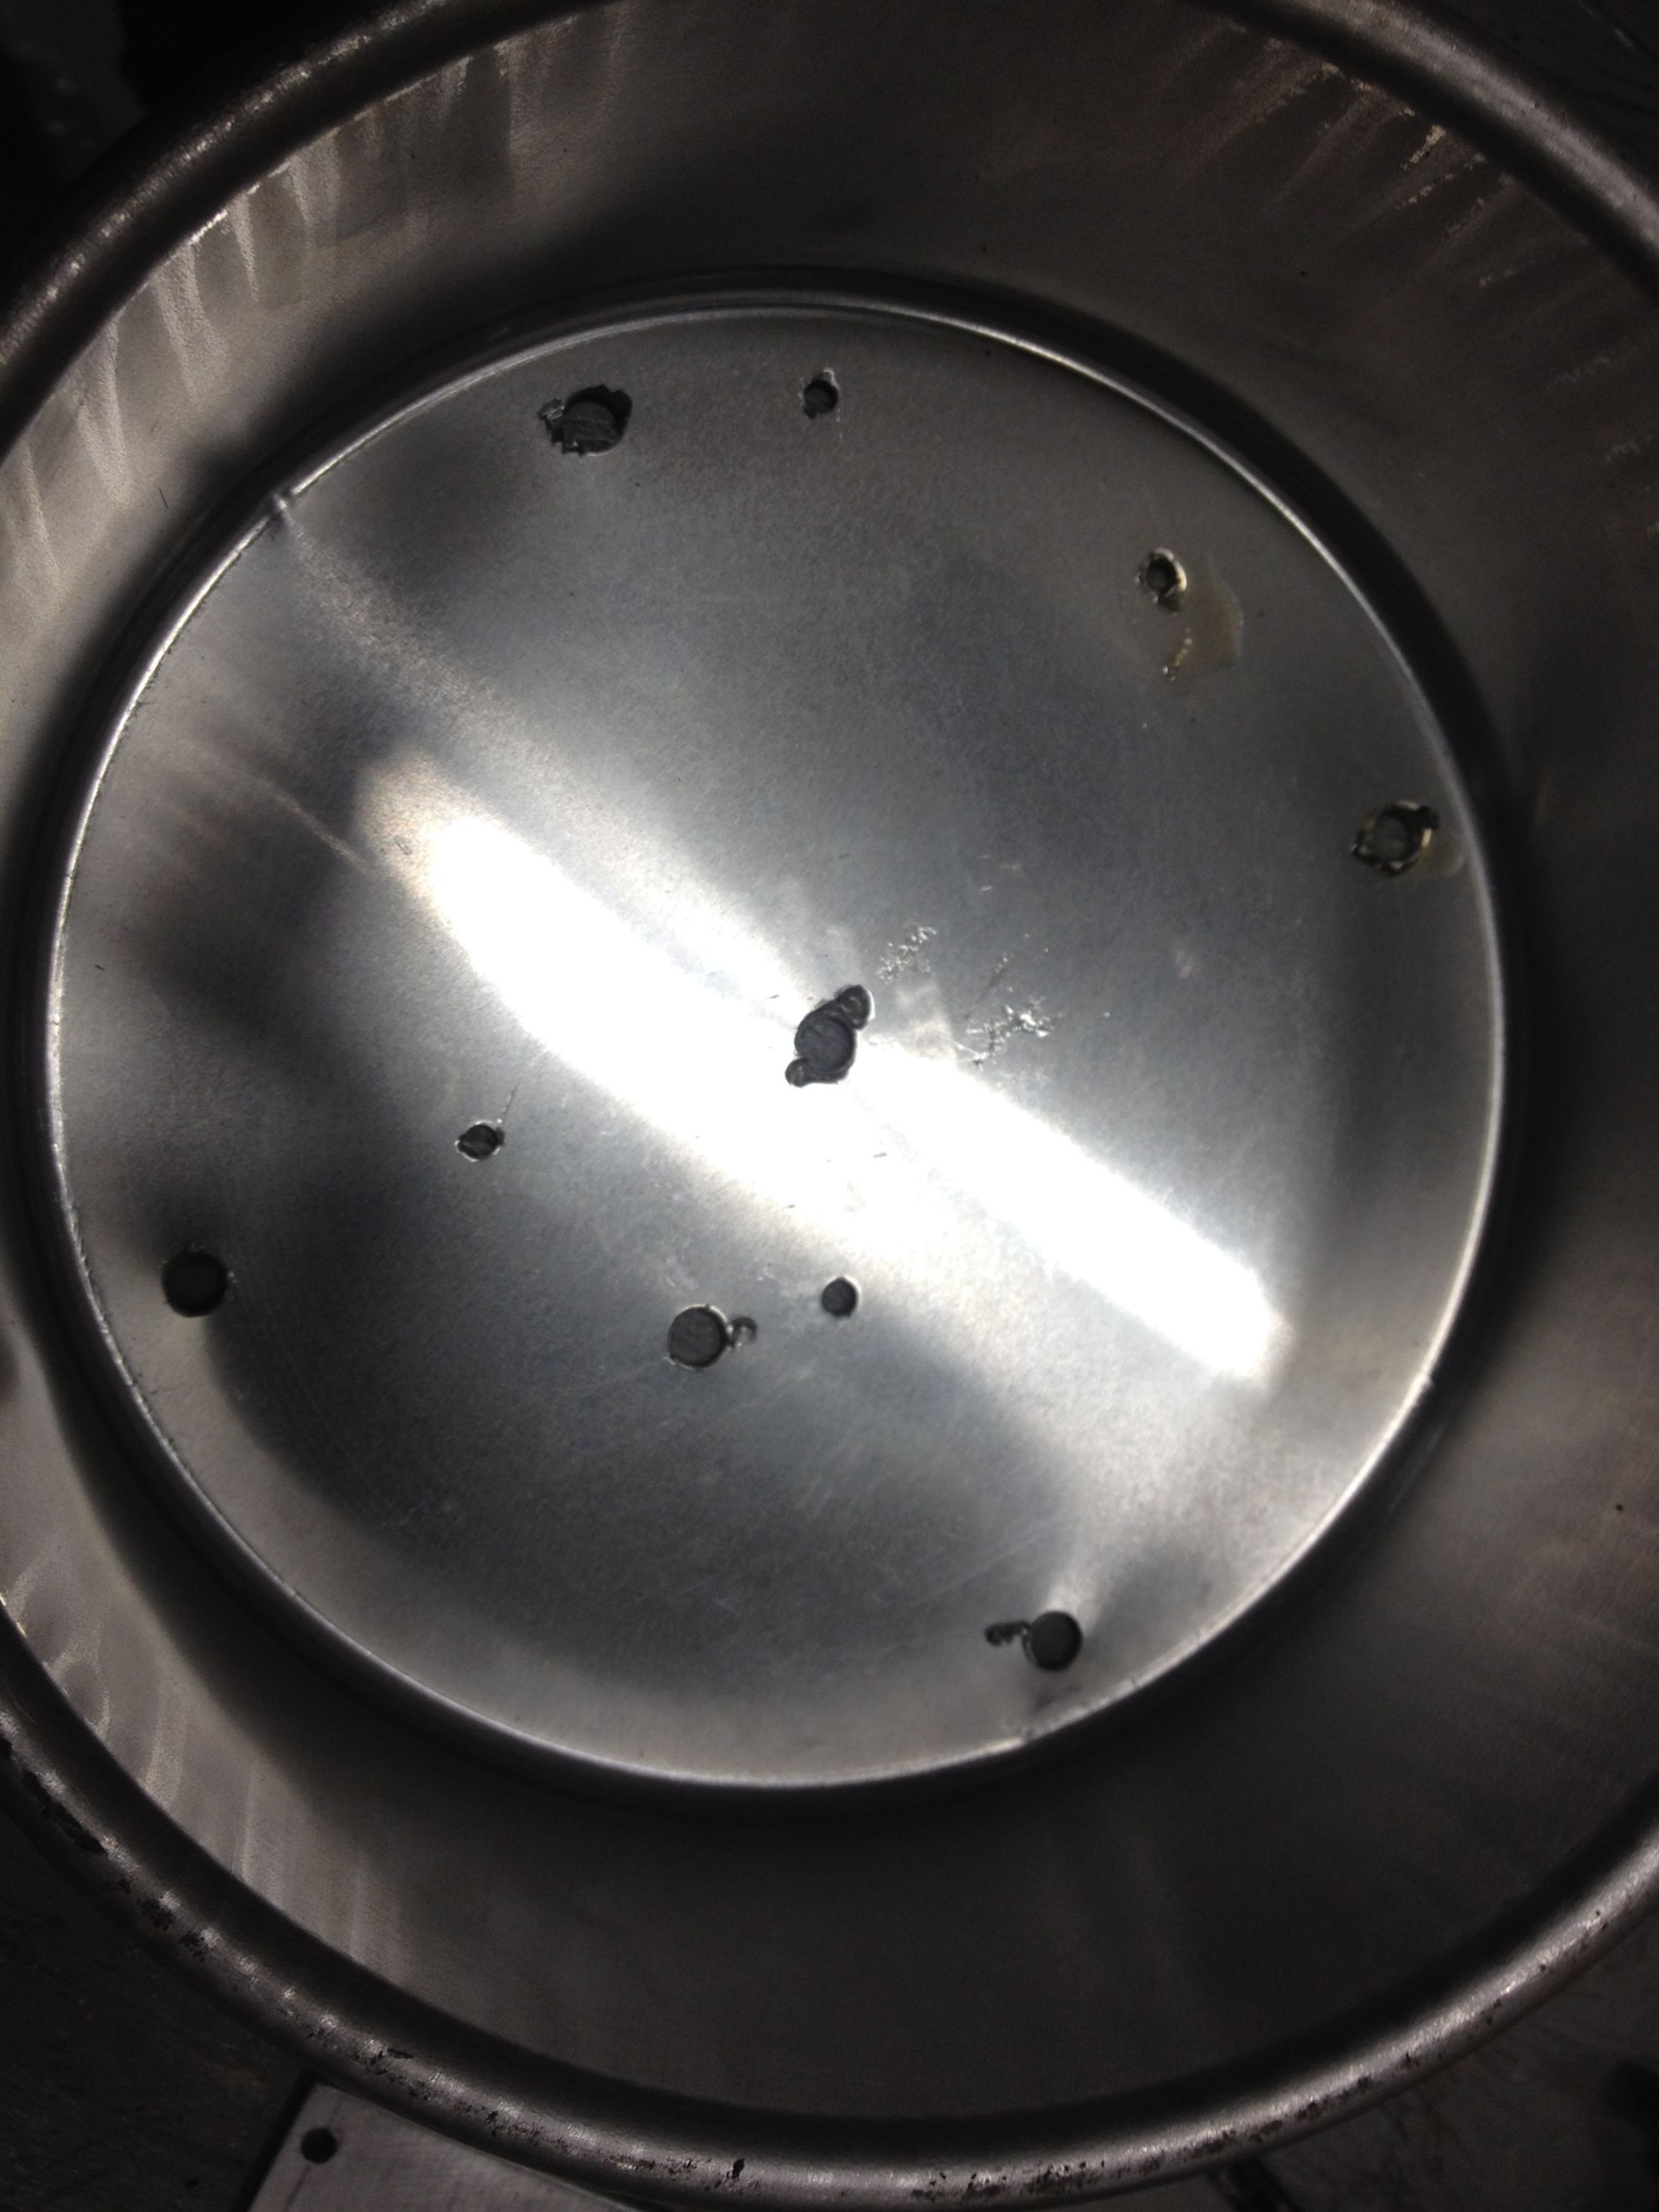
\includegraphics[scale=0.12]{feed/08.jpeg}
\end{center}

\subsubsection{Making helical antenna}
We cut out strips of copper tape with an X-acto knife and a straight edge. 

\begin{center}
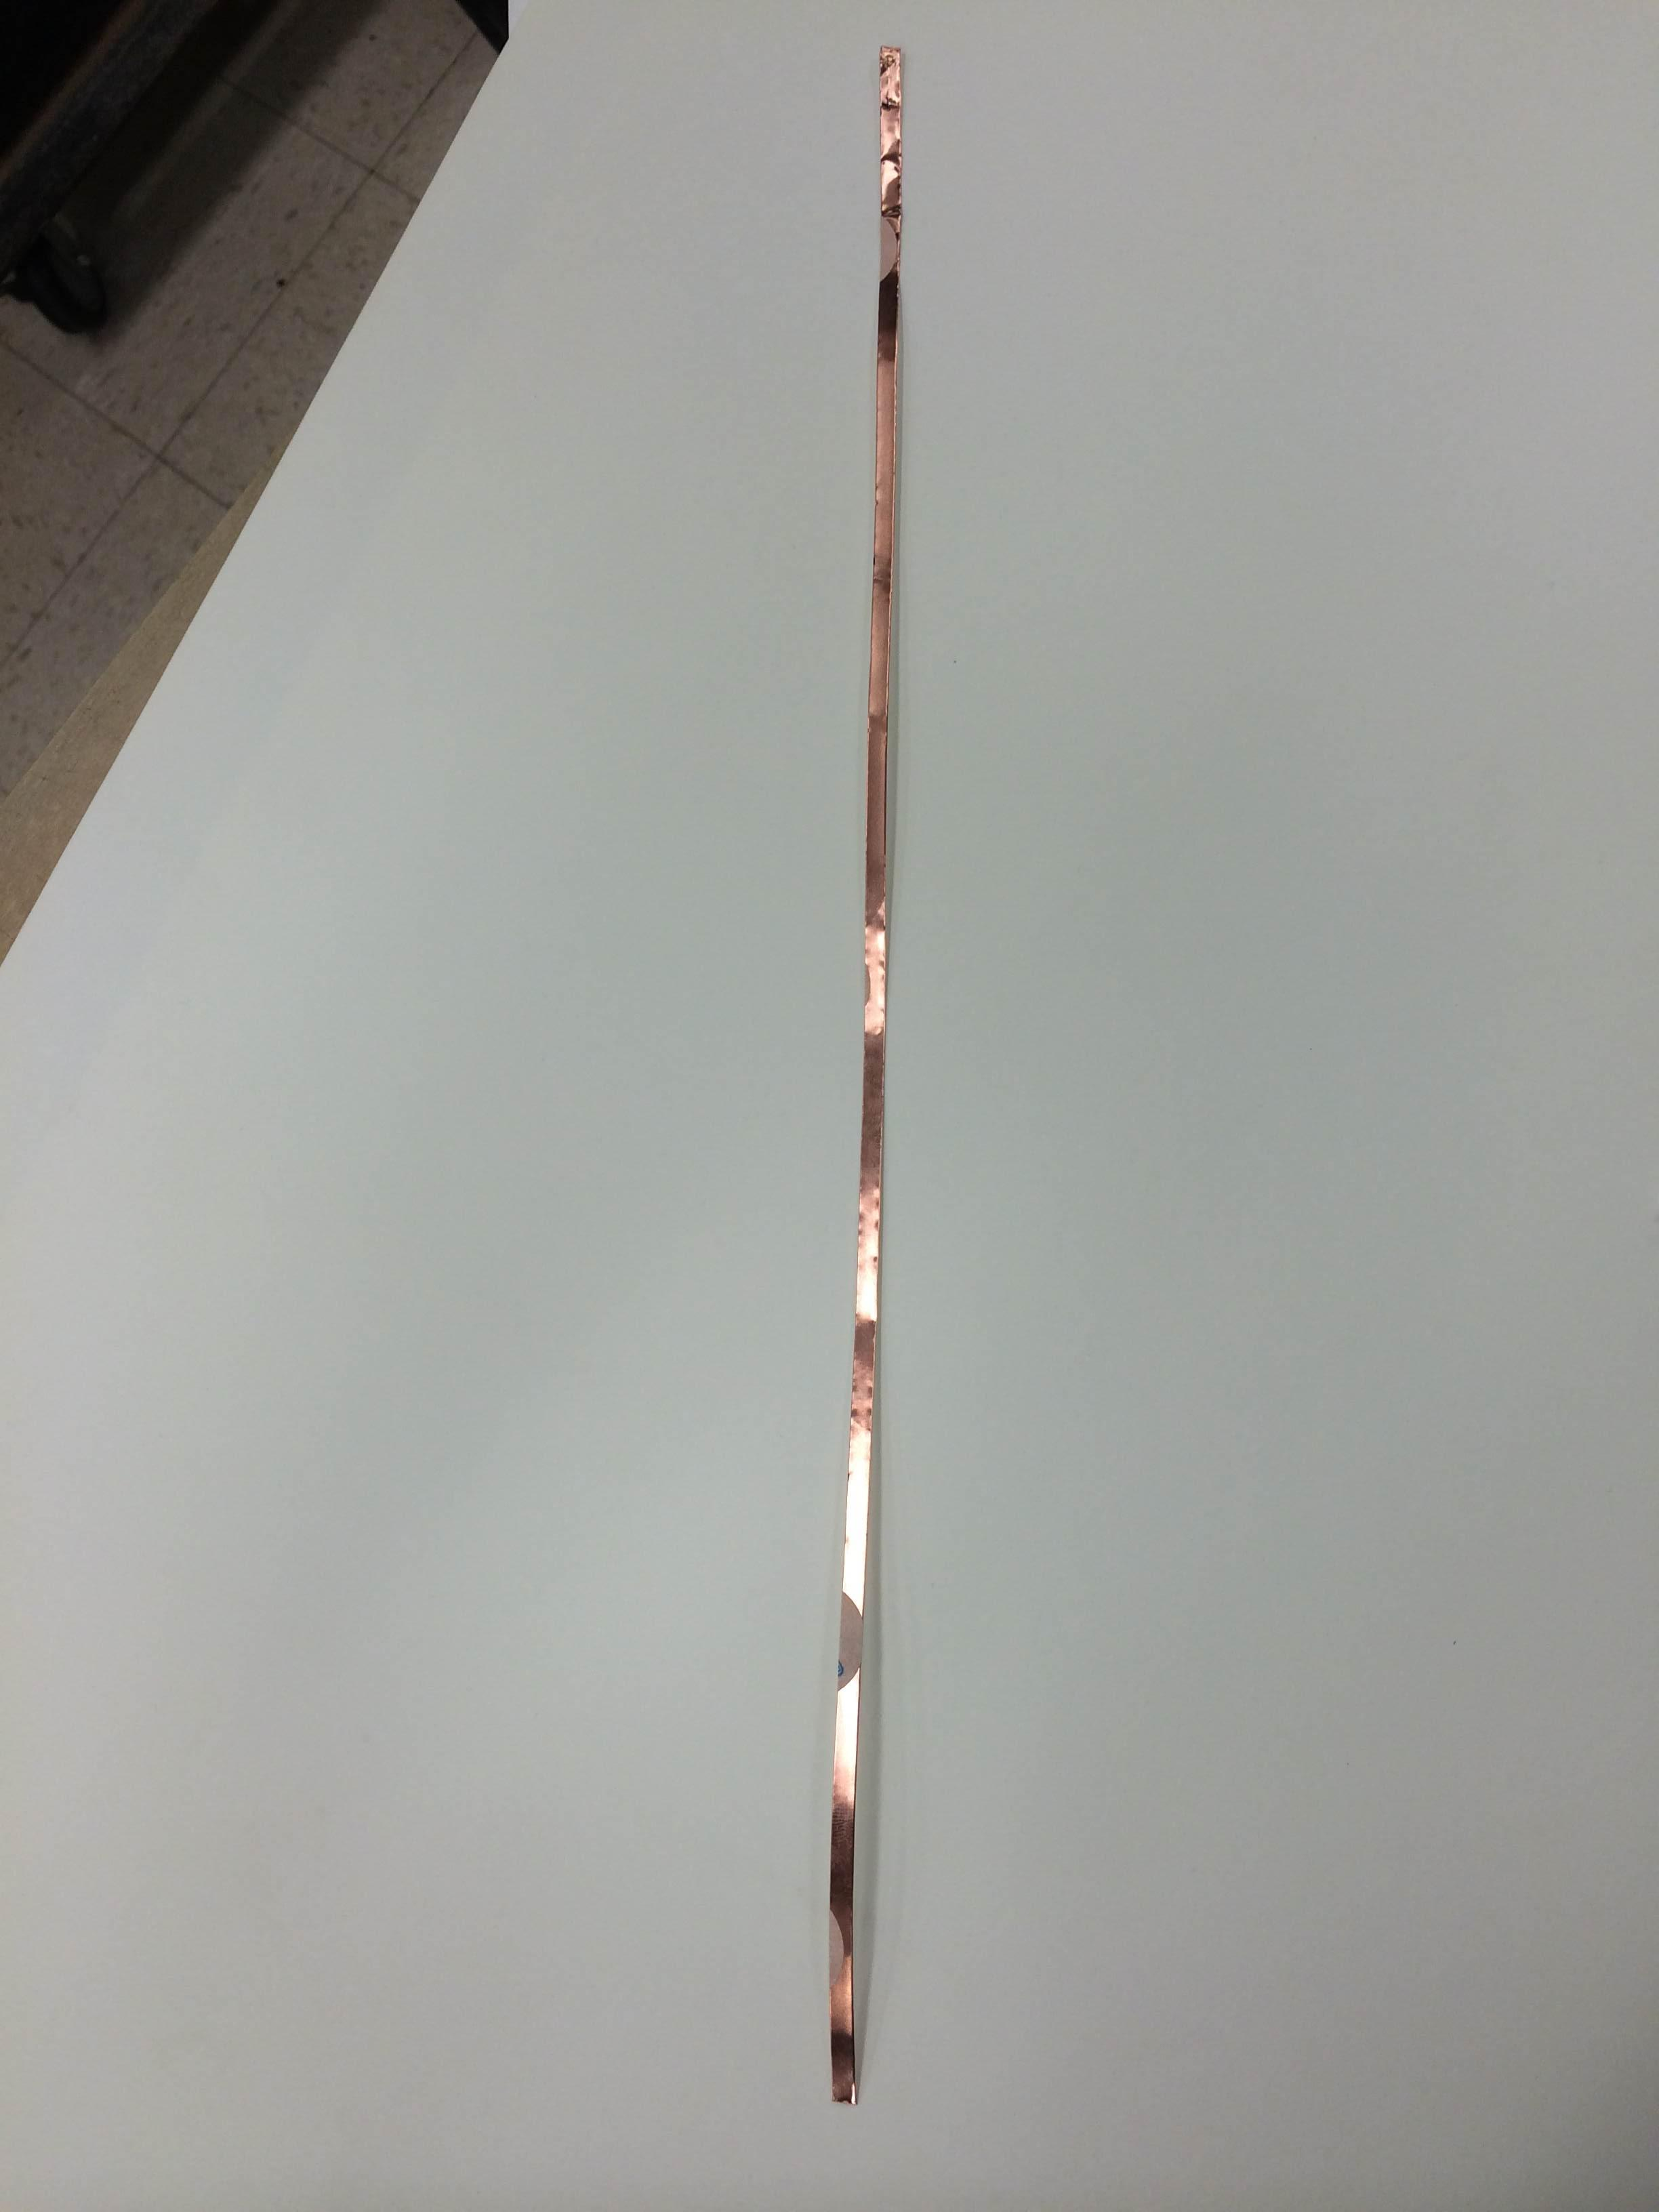
\includegraphics[scale=0.10]{feed/09.jpeg}
\end{center}

Then we measured marked the styrofoam rod at even intervals as specified by the manual to get a consistent helix with the tape. 

\begin{center}
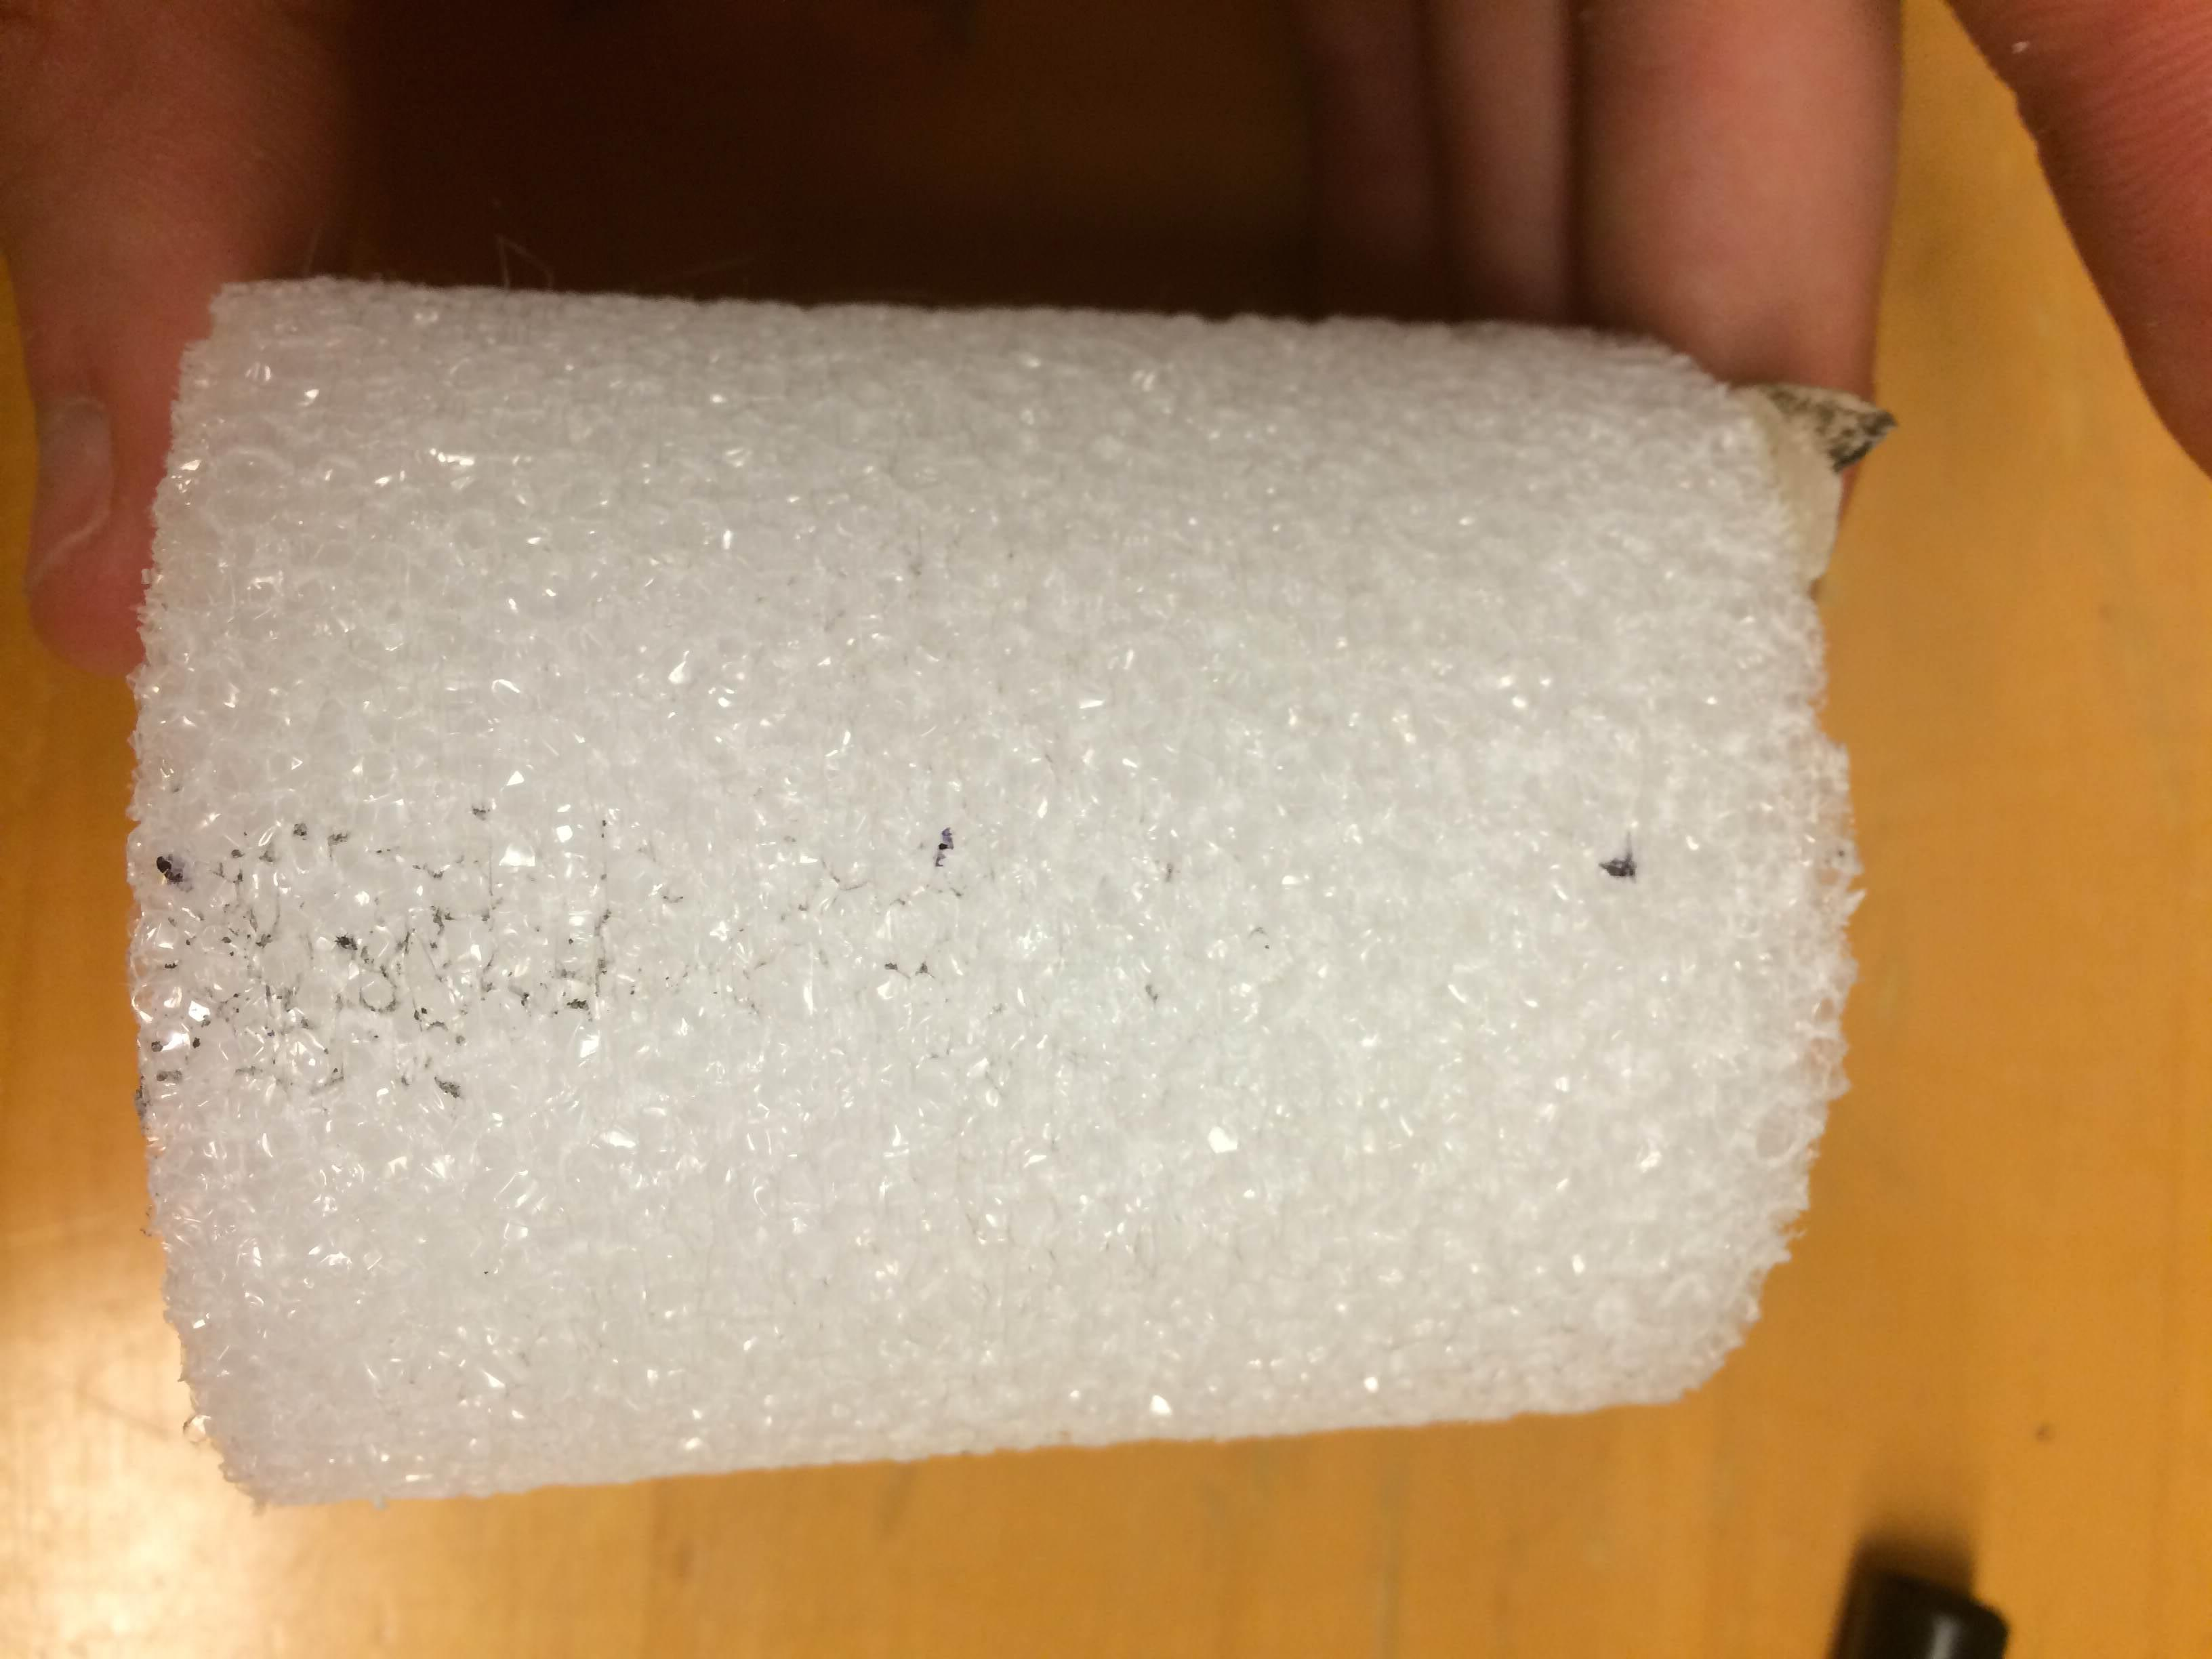
\includegraphics[scale=0.08]{feed/10.jpeg}
\end{center}

\begin{center}
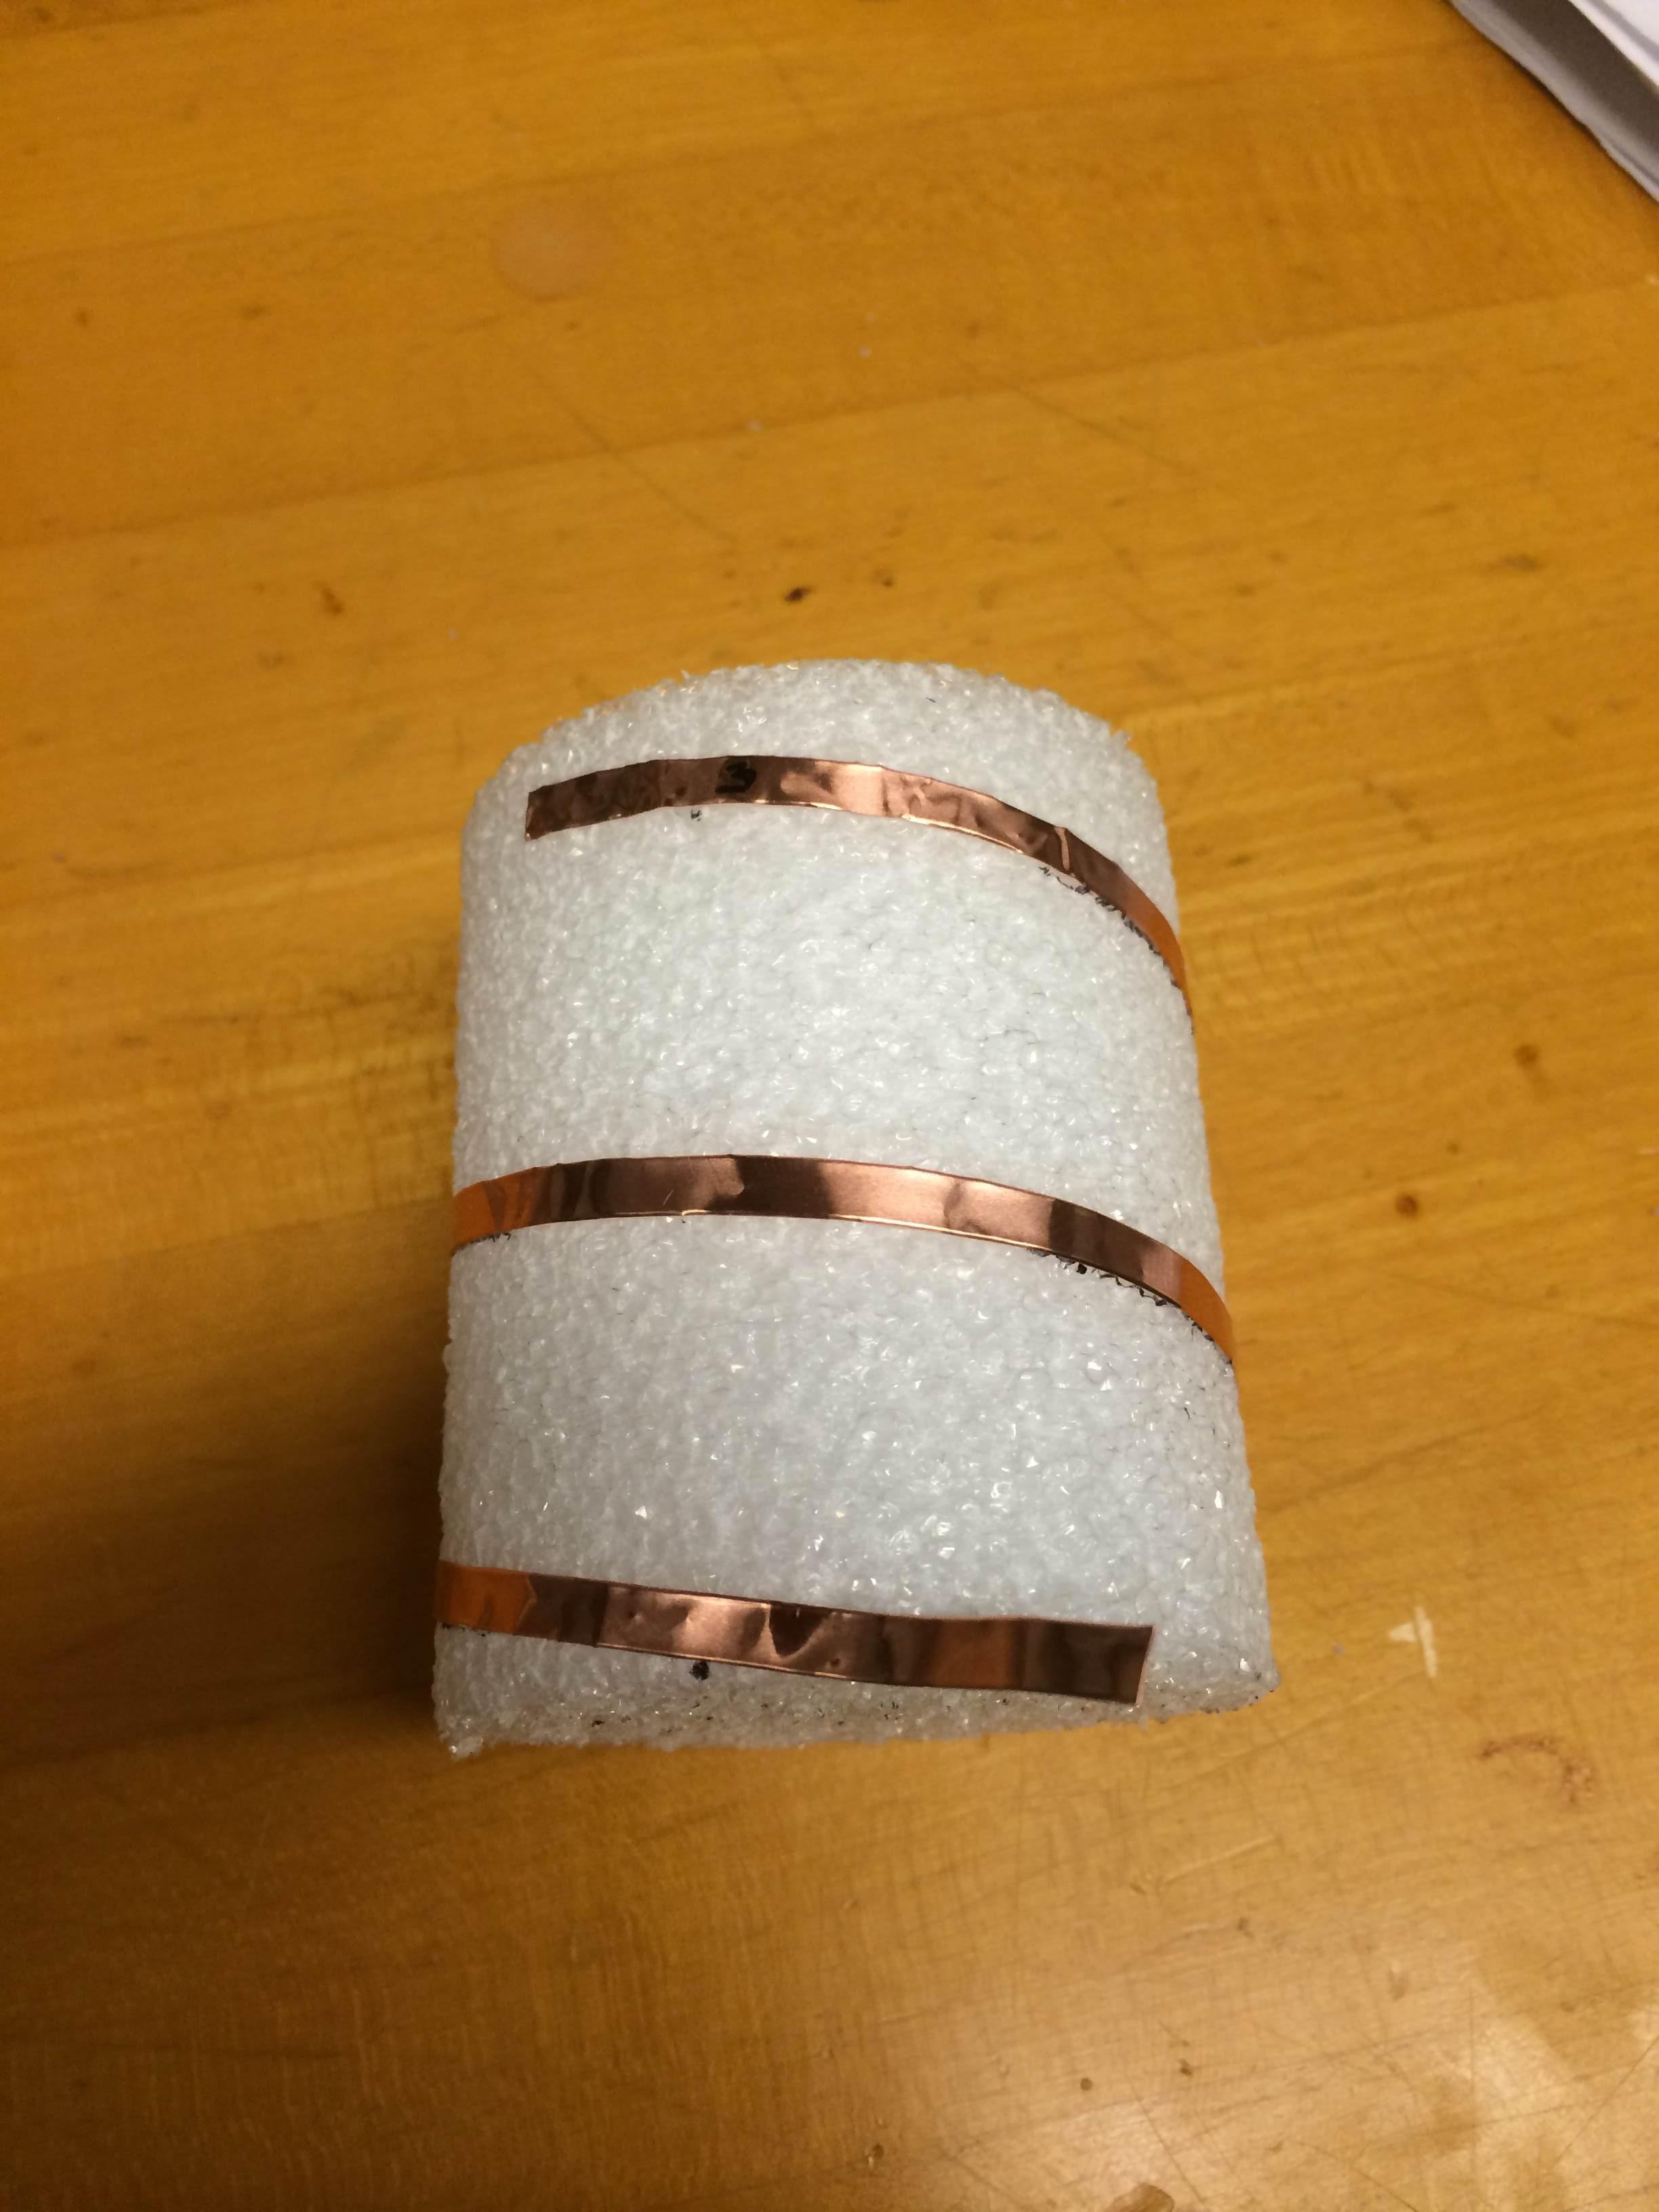
\includegraphics[scale=0.08]{feed/11.jpeg}
\end{center}


Once the tape was applied we soldered on 26.25mmx13mm piece of copper tape for impedance matching section. Note: It is important to include an extra 3-4mm on the long side of the rectangle so that it can be attached to the helix. 


In the process we melted some of the rod. This should be ok as long as the tape stays in a helix. 

\begin{center}
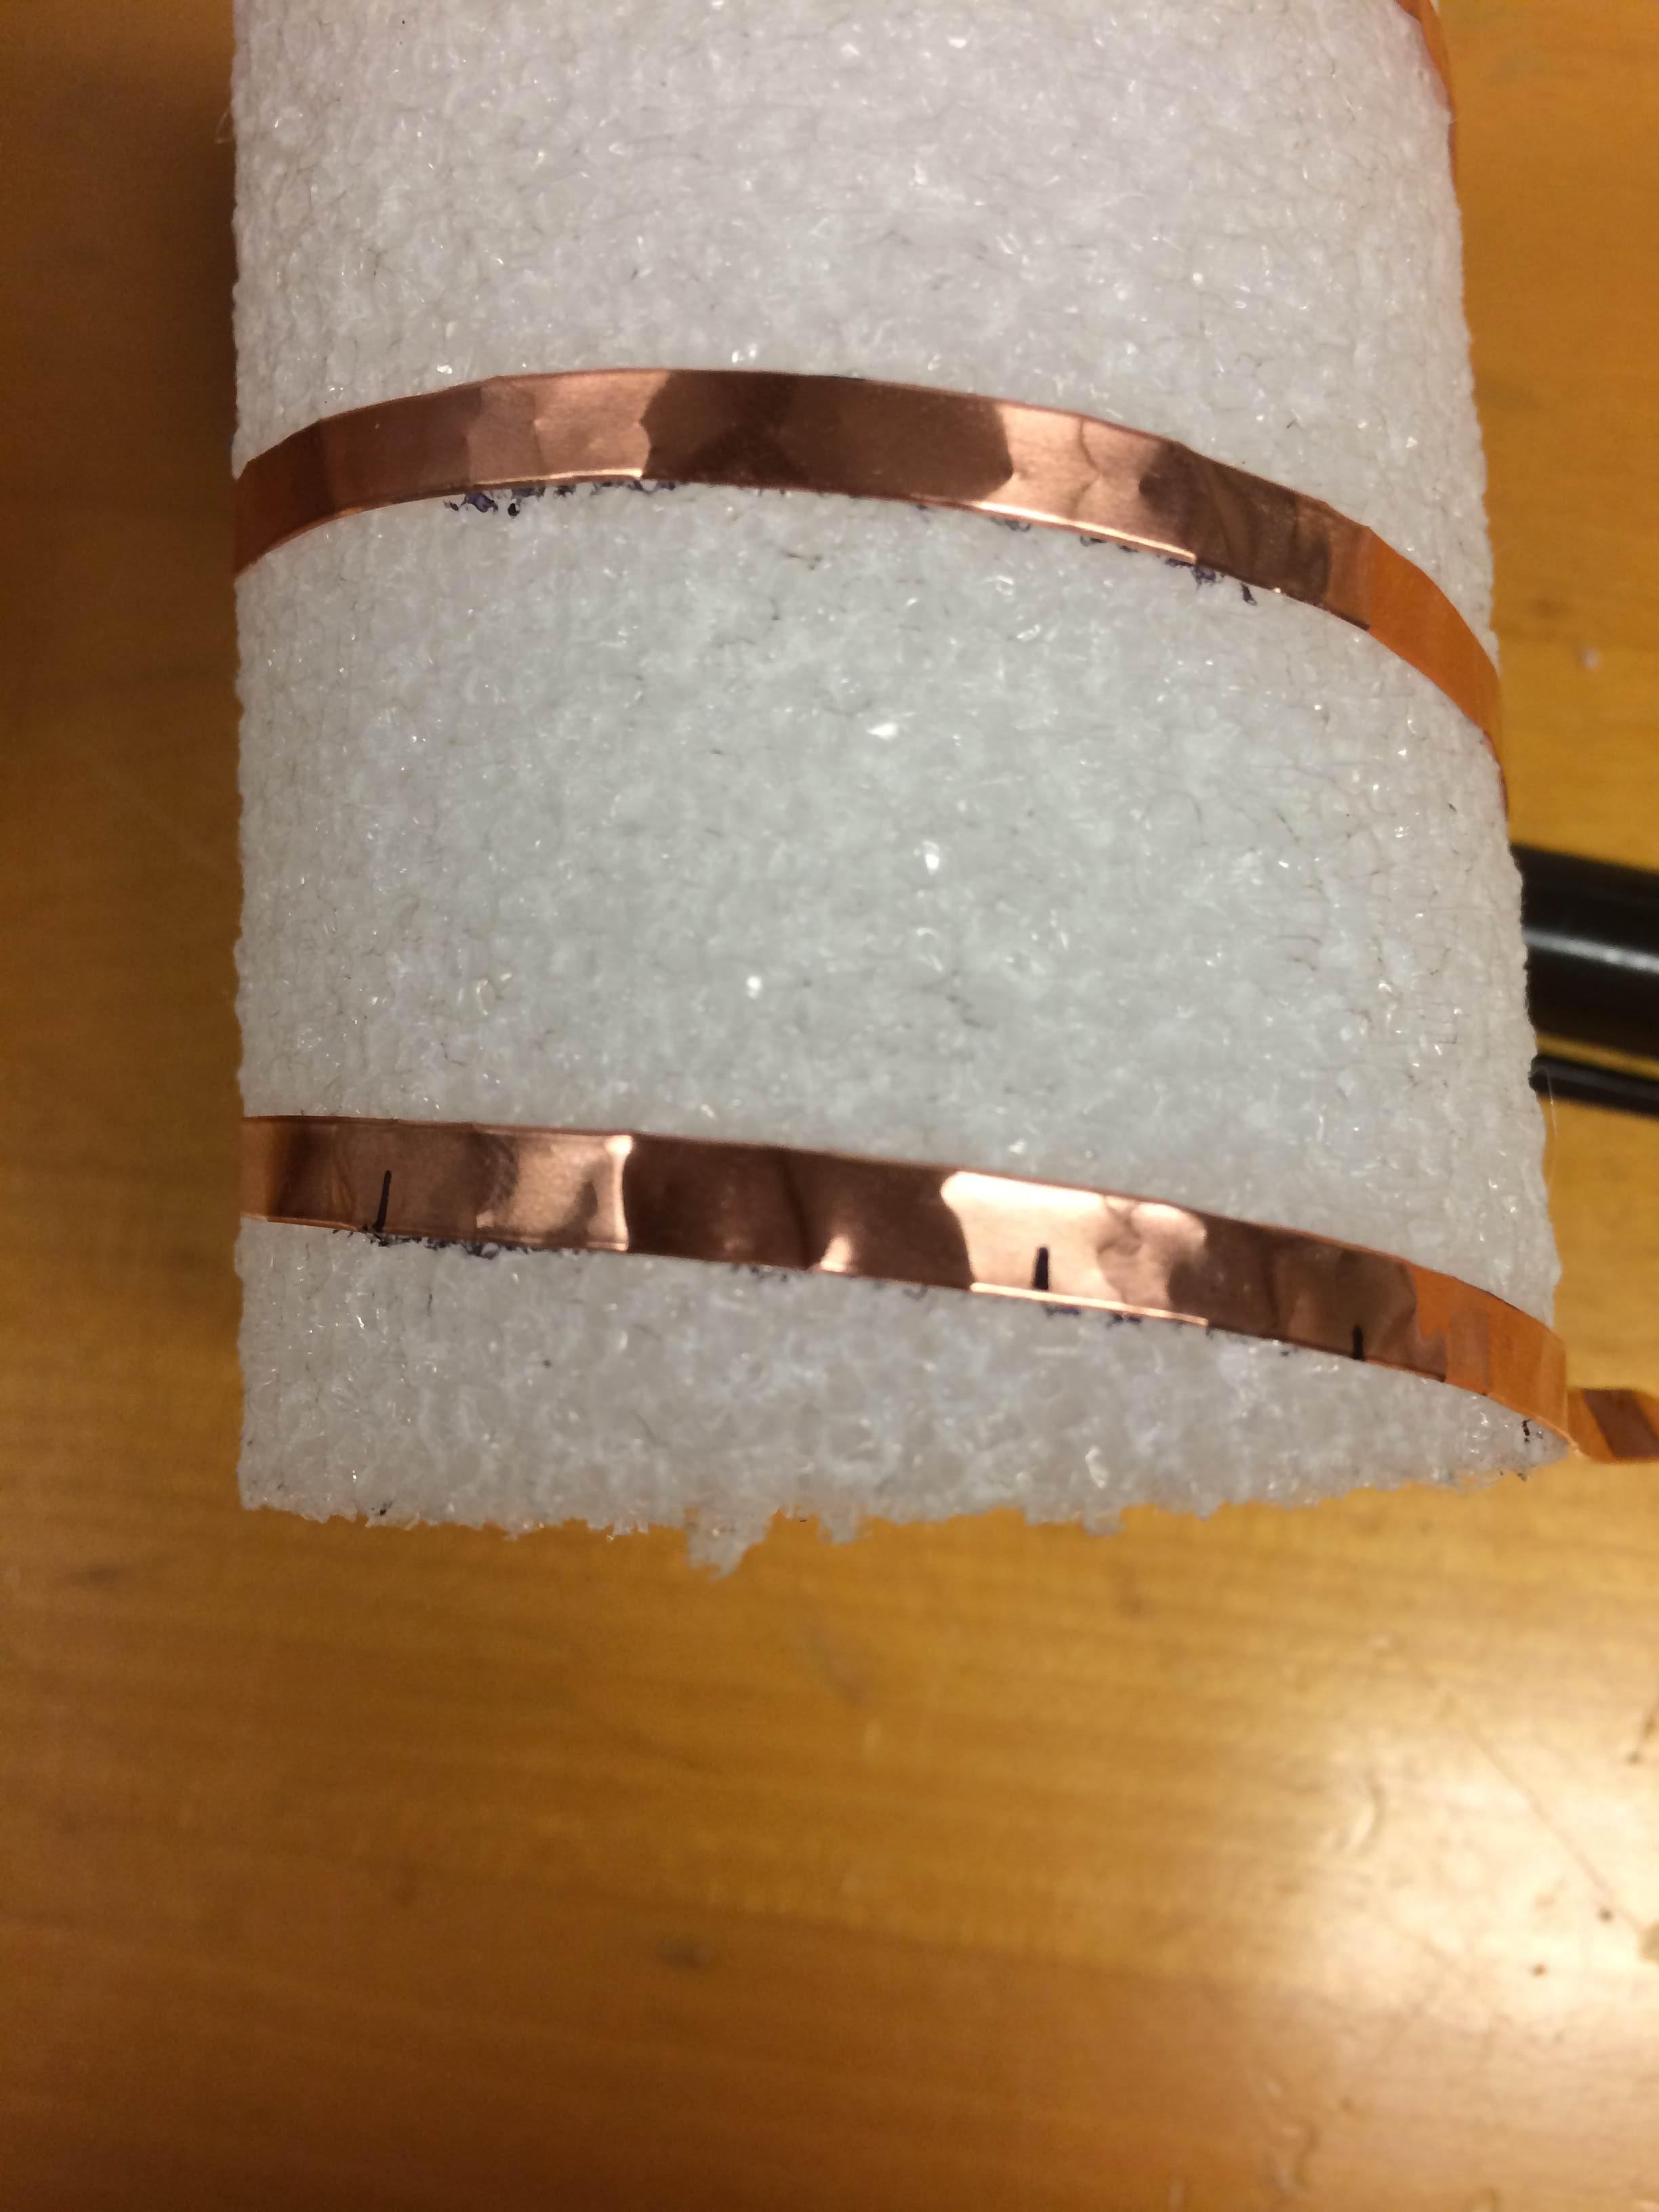
\includegraphics[scale=0.14]{feed/12.jpeg}
\end{center}


\begin{center}
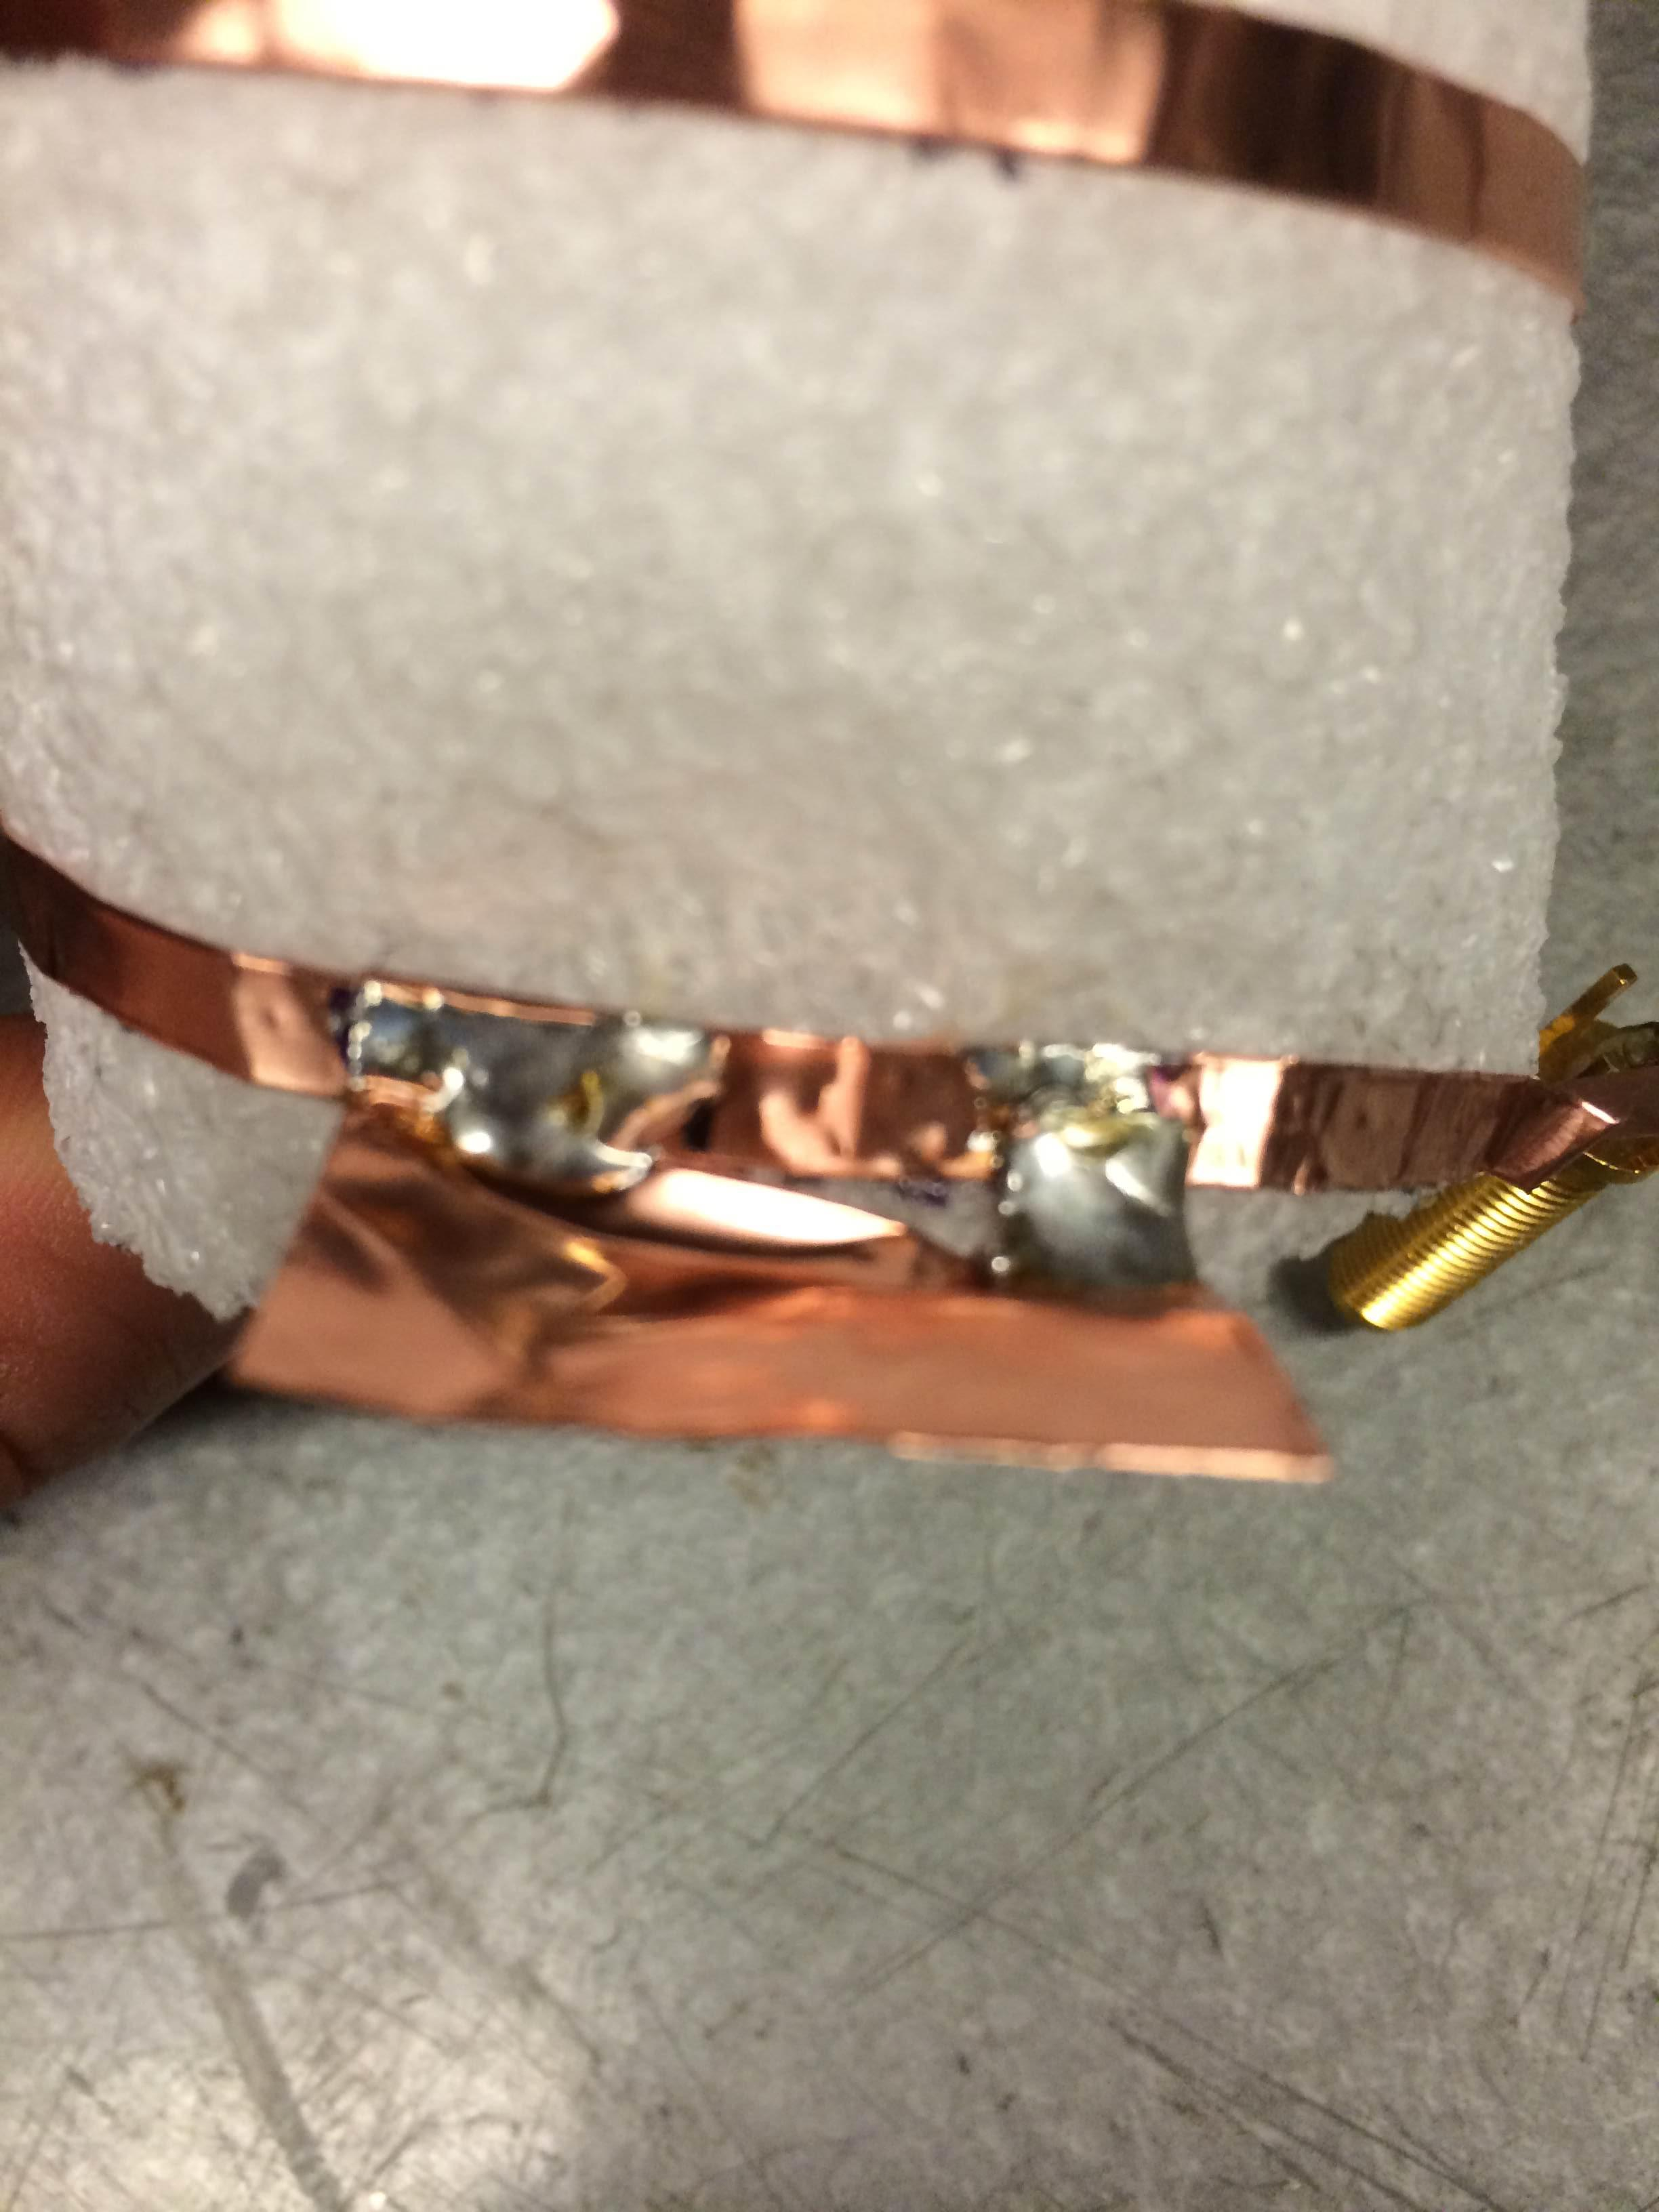
\includegraphics[scale=0.10]{feed/13.jpeg}
\end{center}


The we soldered the end of the helix to the SMA connector. MIT cut off some of the ground pins to make that easier. We left them on and it worked out the same. 

\begin{center}
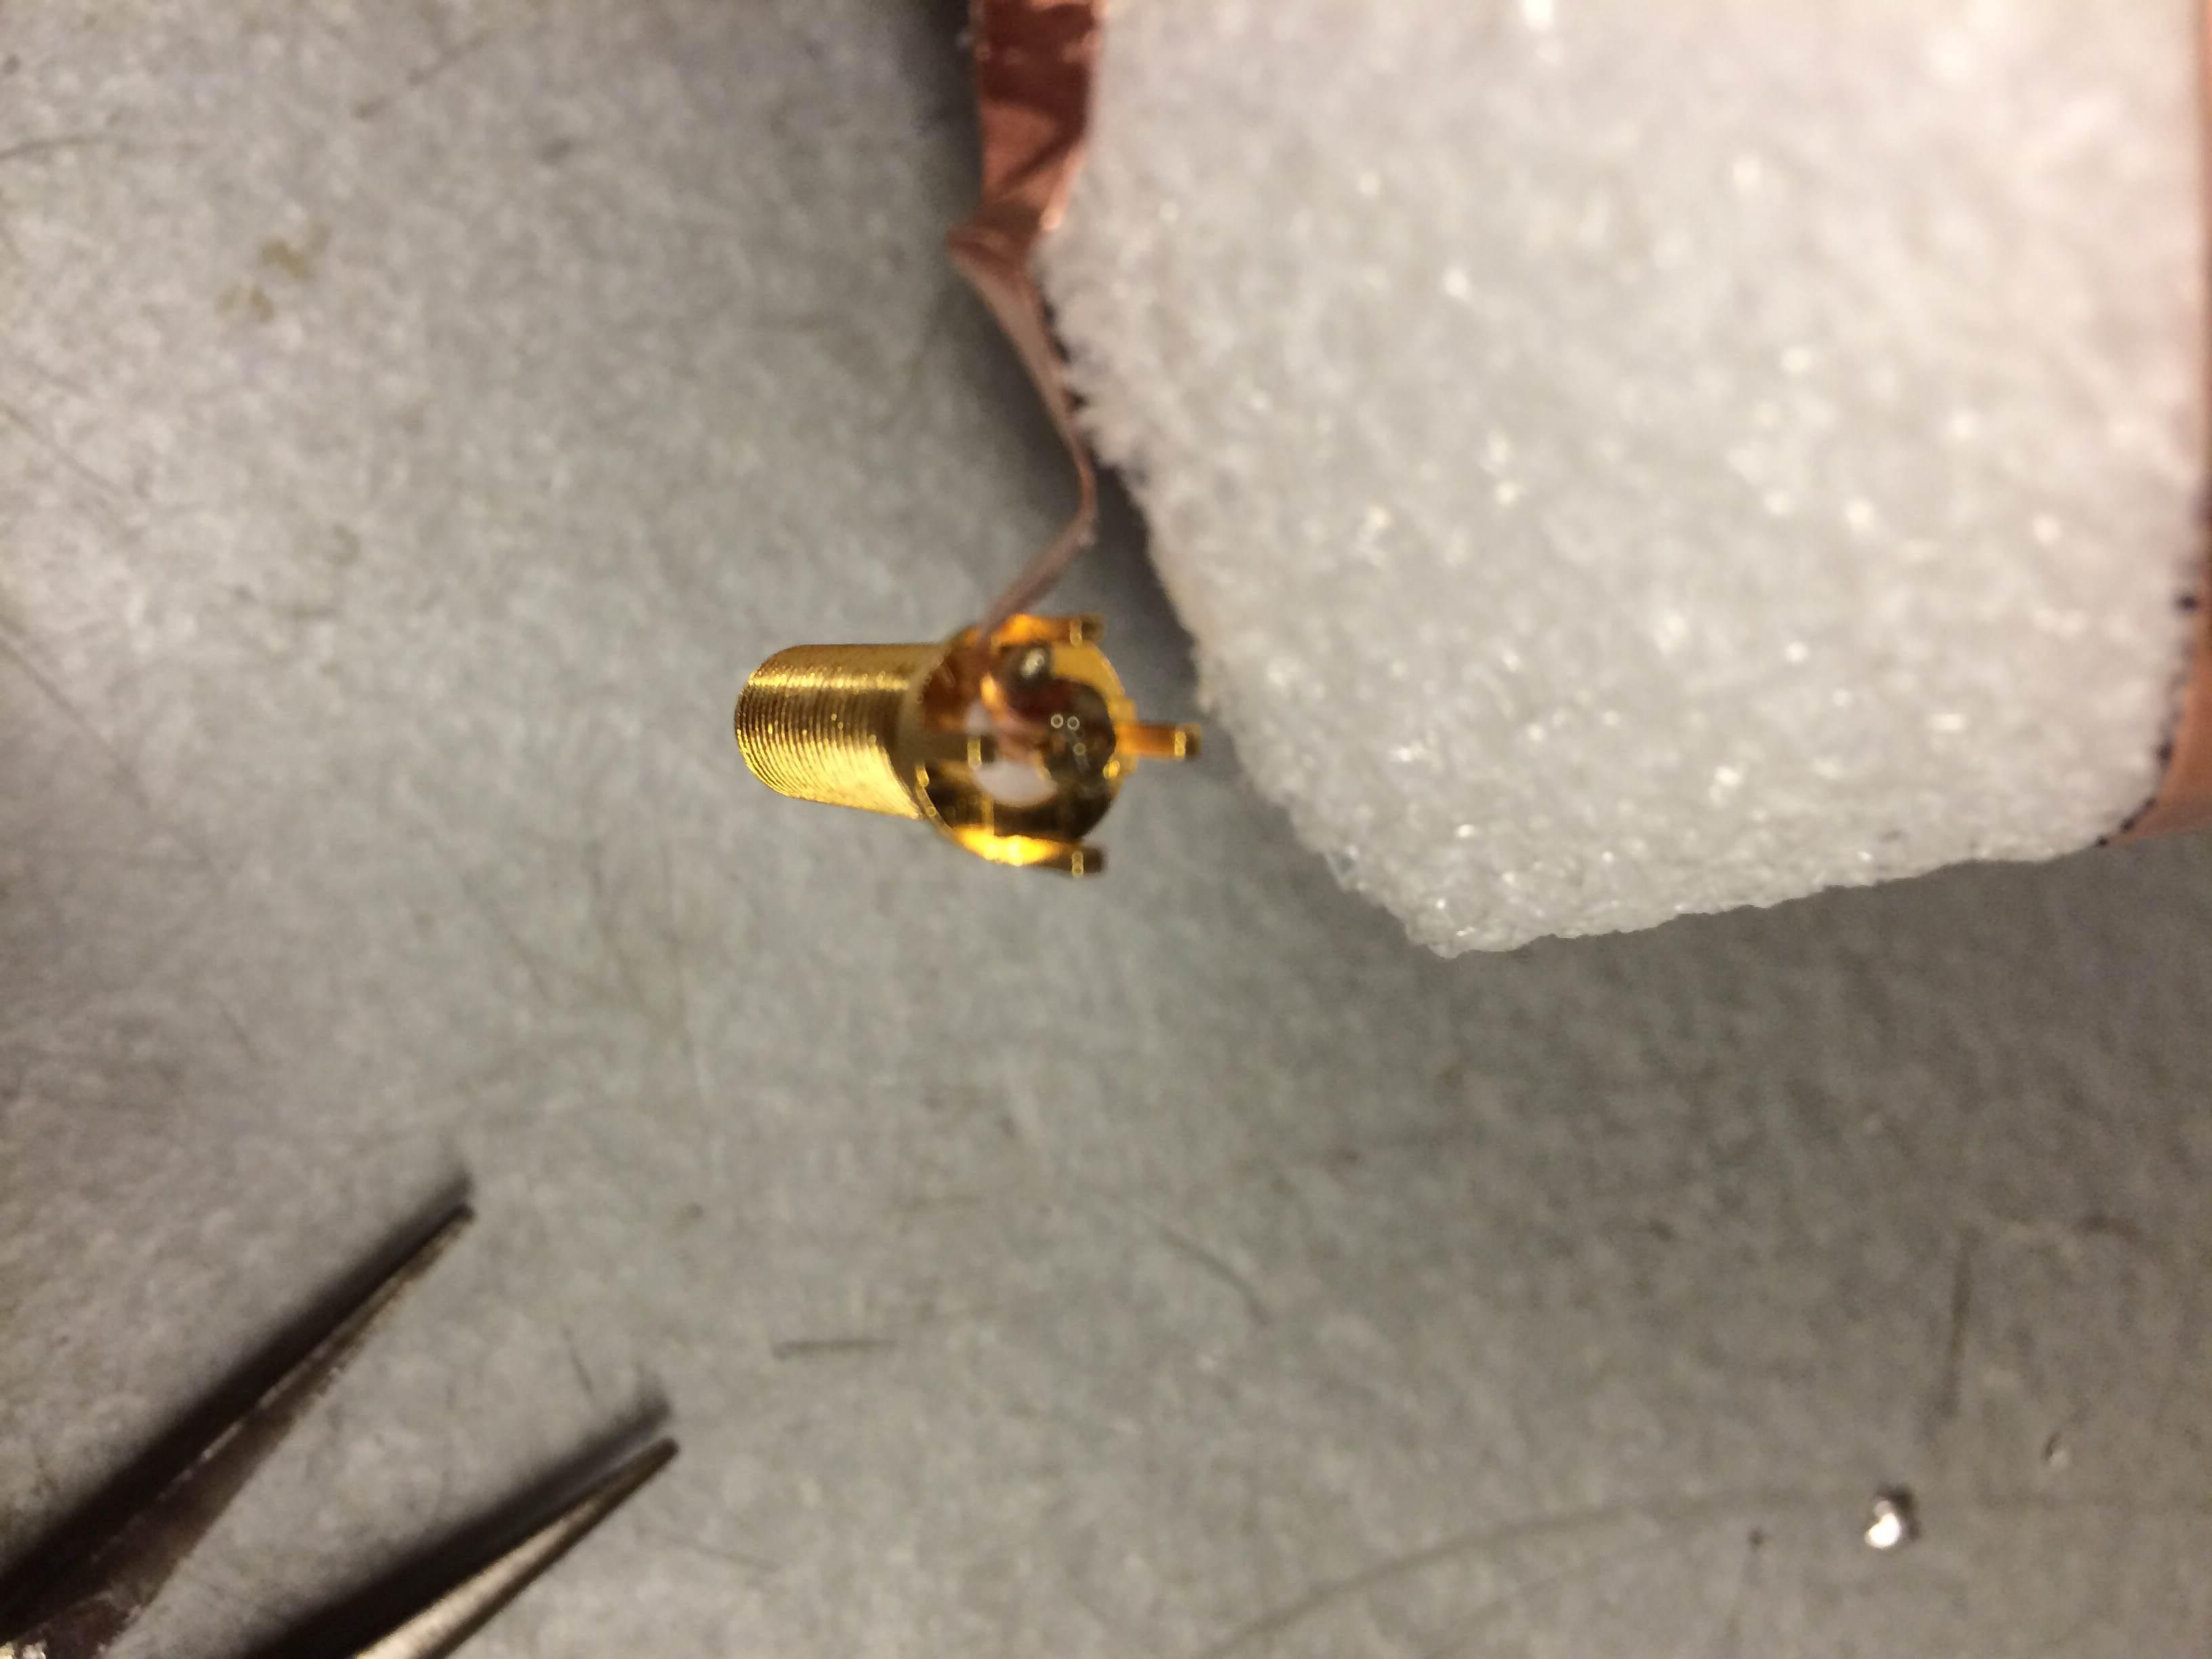
\includegraphics[scale=0.10]{feed/14.jpeg}
\end{center}


\subsubsection{Drilling/cutting PC board}
We cut the PC board into 63mm squares (We had enough PC board to make a couple back ups). 

\begin{center}
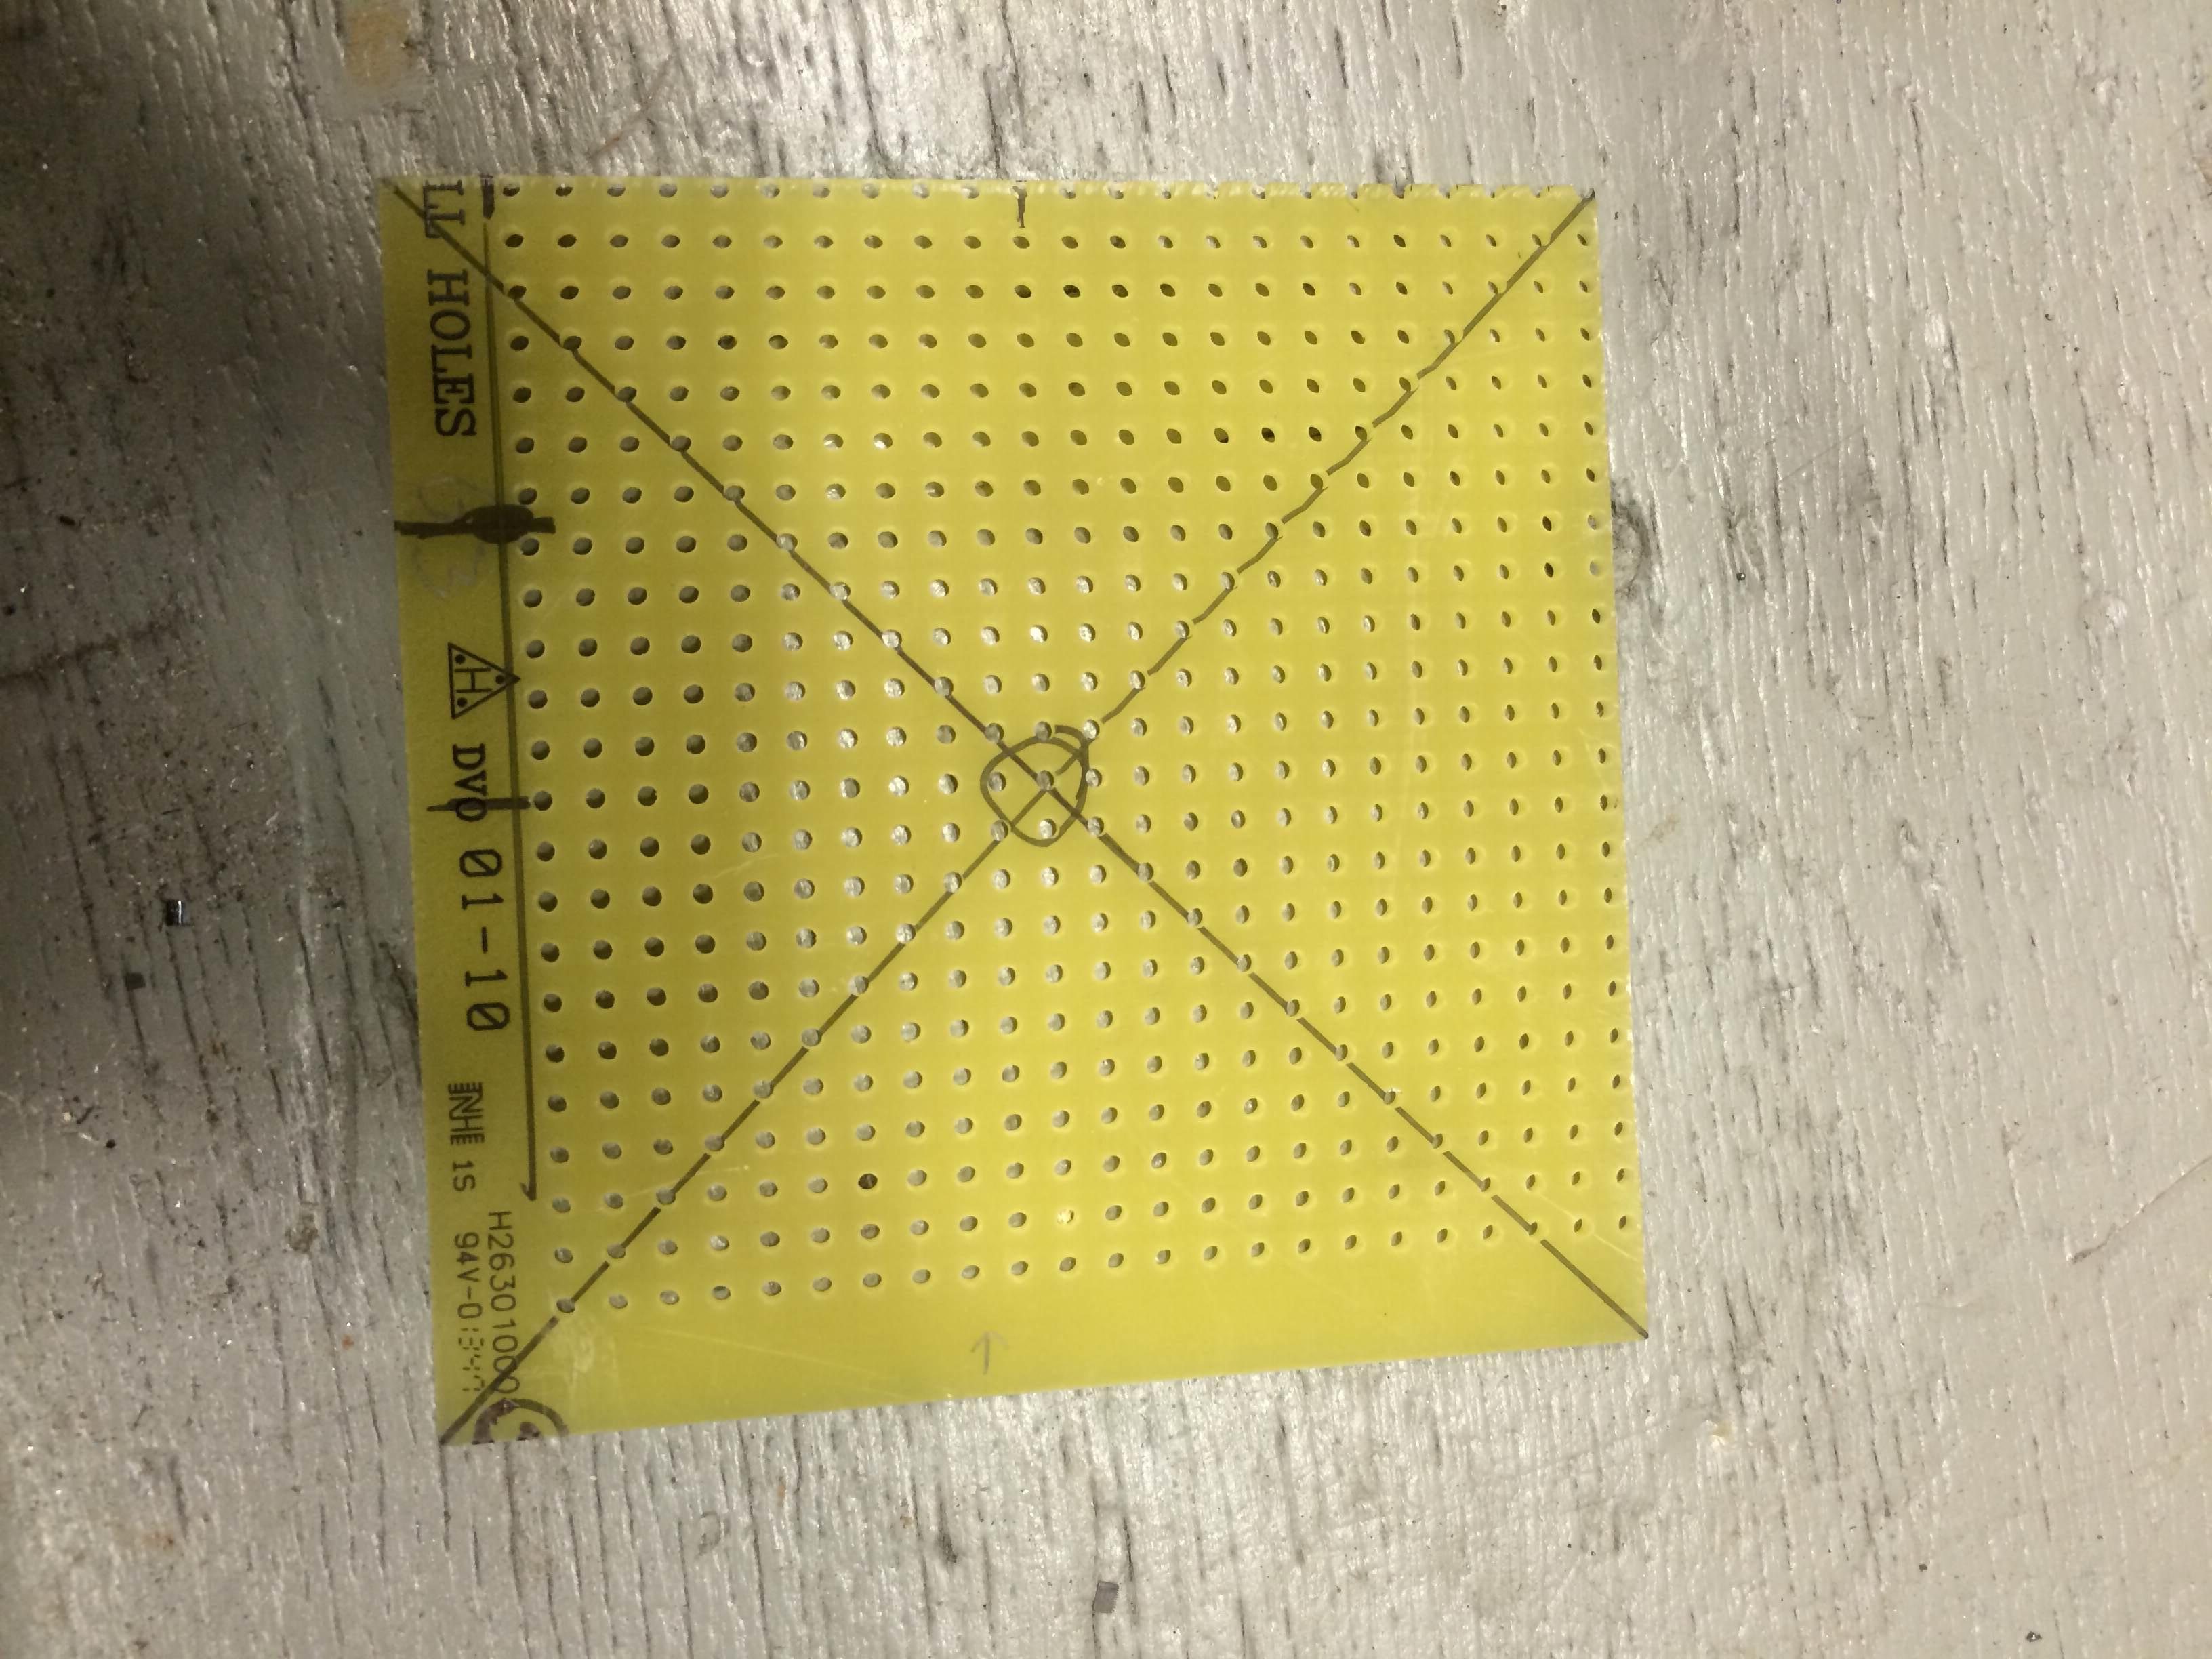
\includegraphics[scale=0.08]{feed/15.jpeg}
\end{center}


Then we drilled holes in it as specified by the manual using a drill press. It was relatively easy to secure the board in a vice for drilling. 

\begin{center}
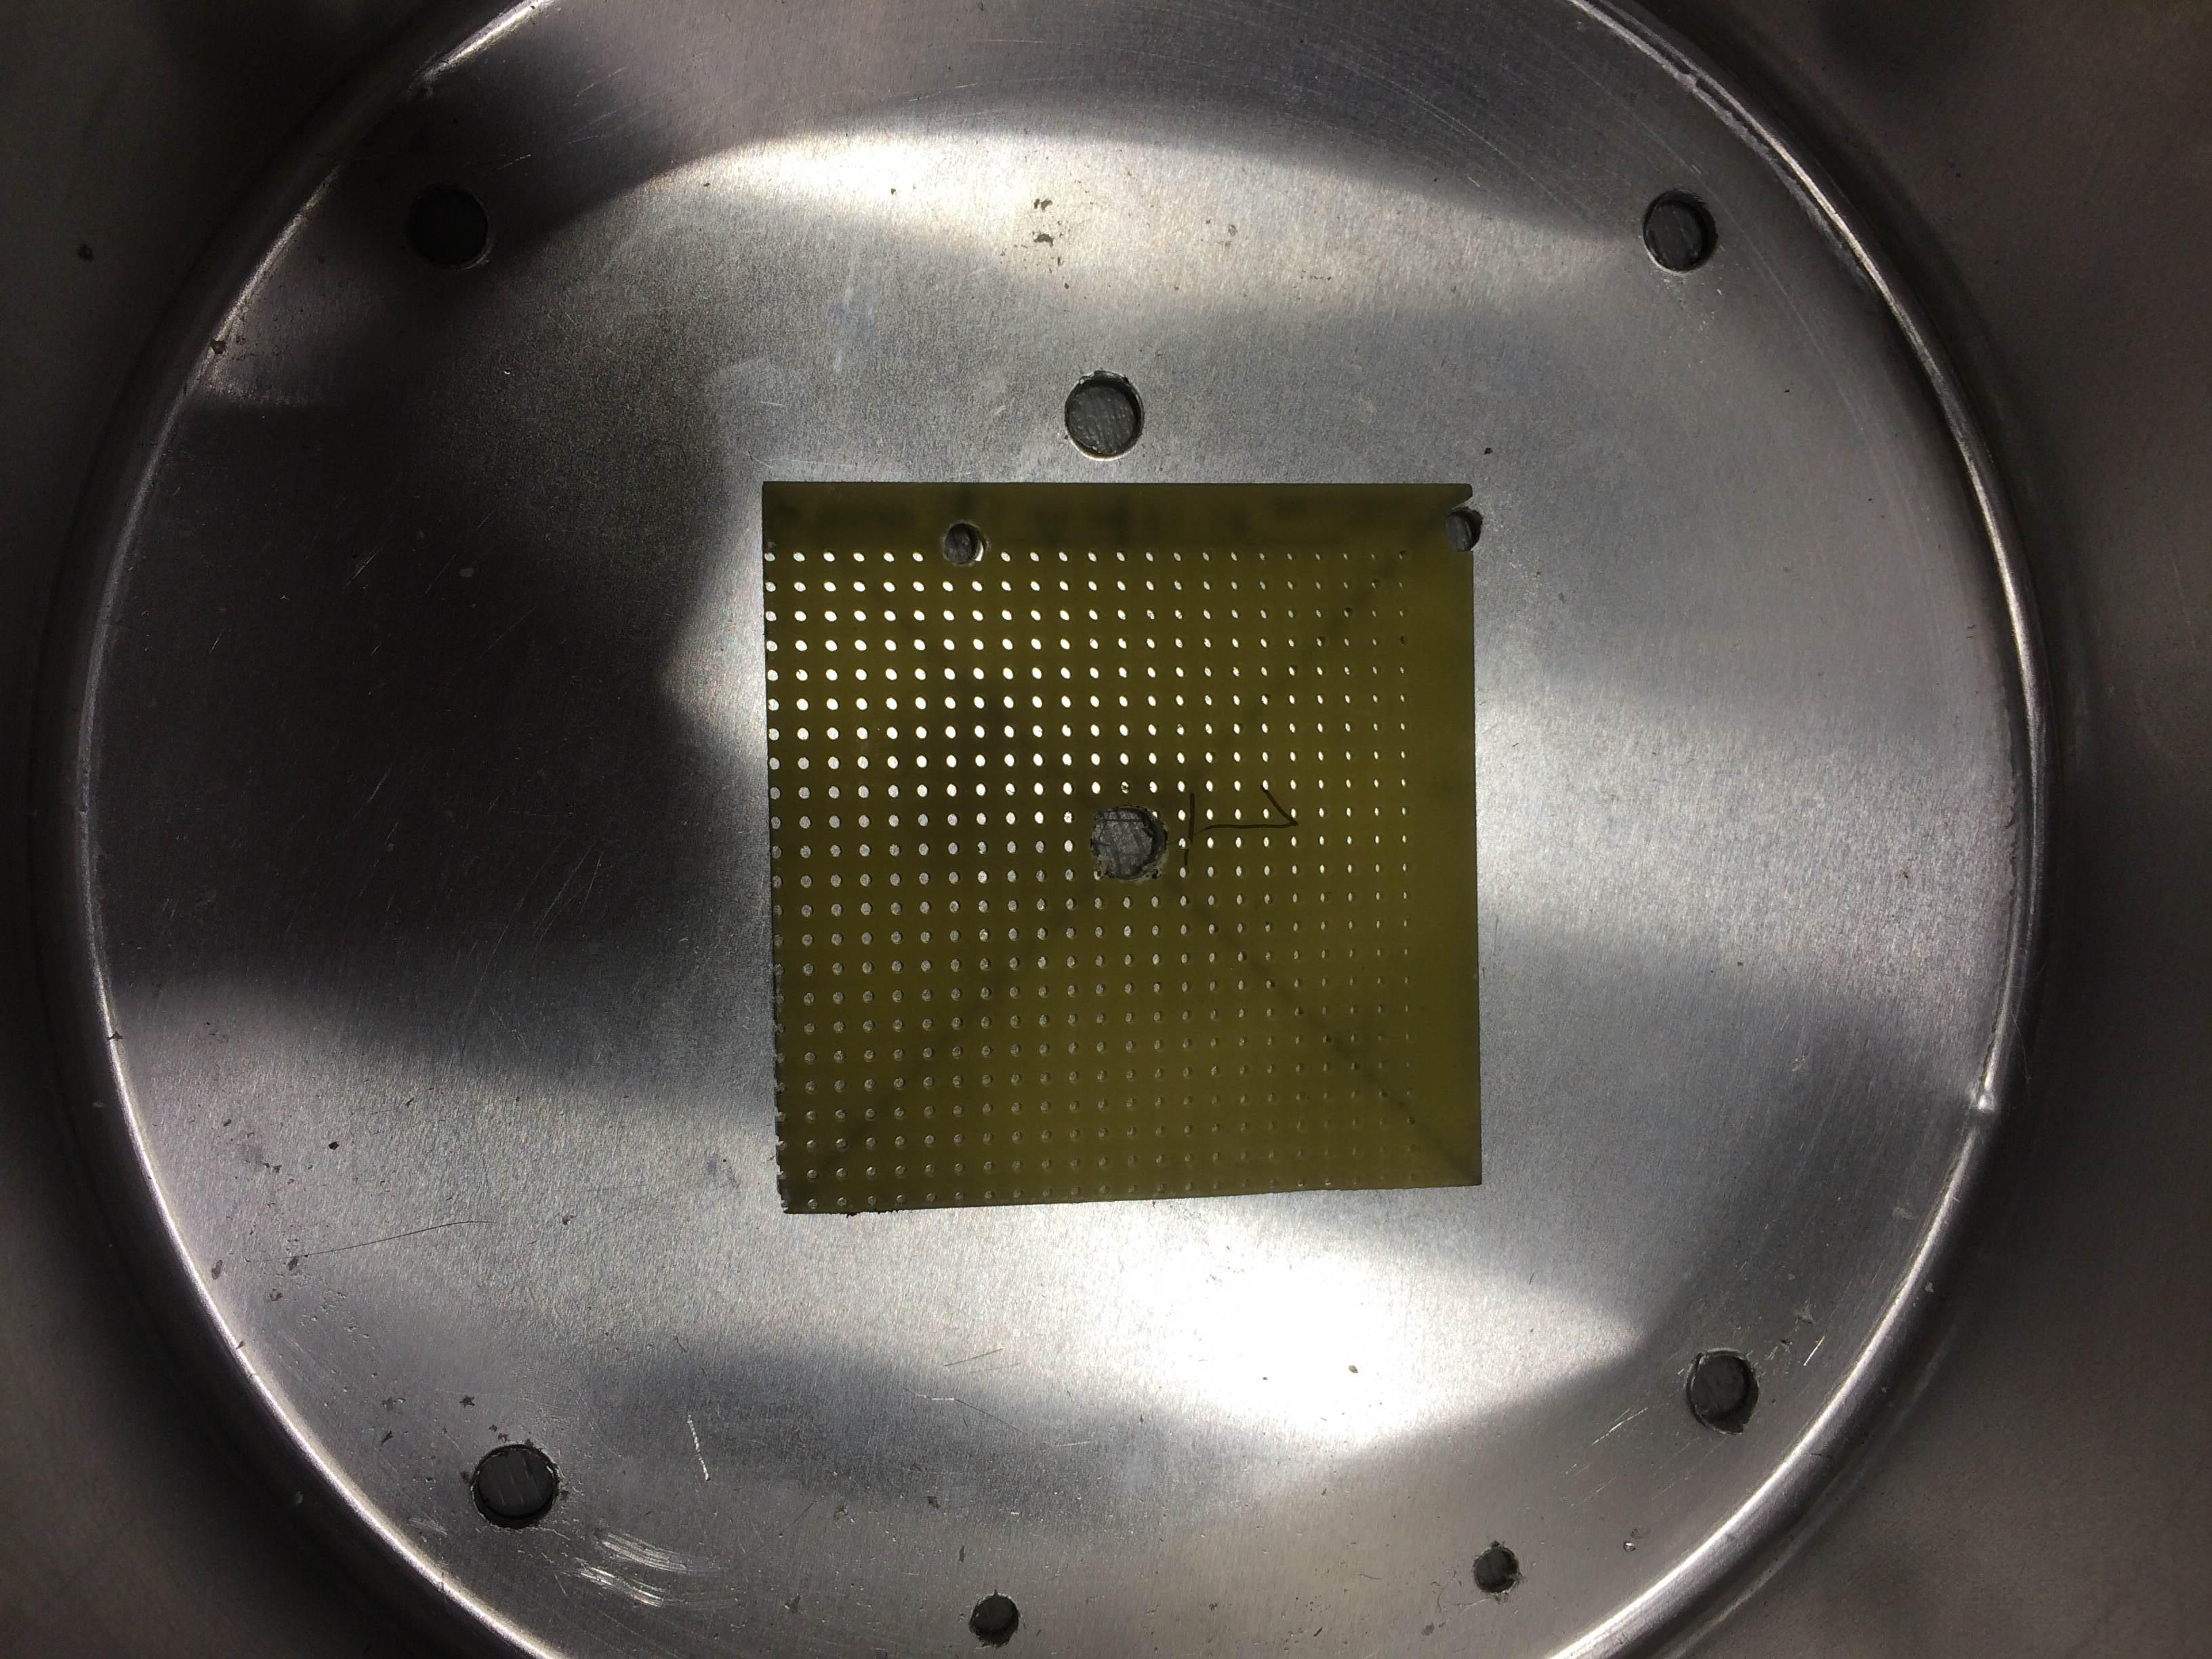
\includegraphics[scale=0.08]{feed/16.jpeg}
\end{center}


\subsubsection{Assembly}
All the components were then bolted together. 

\begin{center}
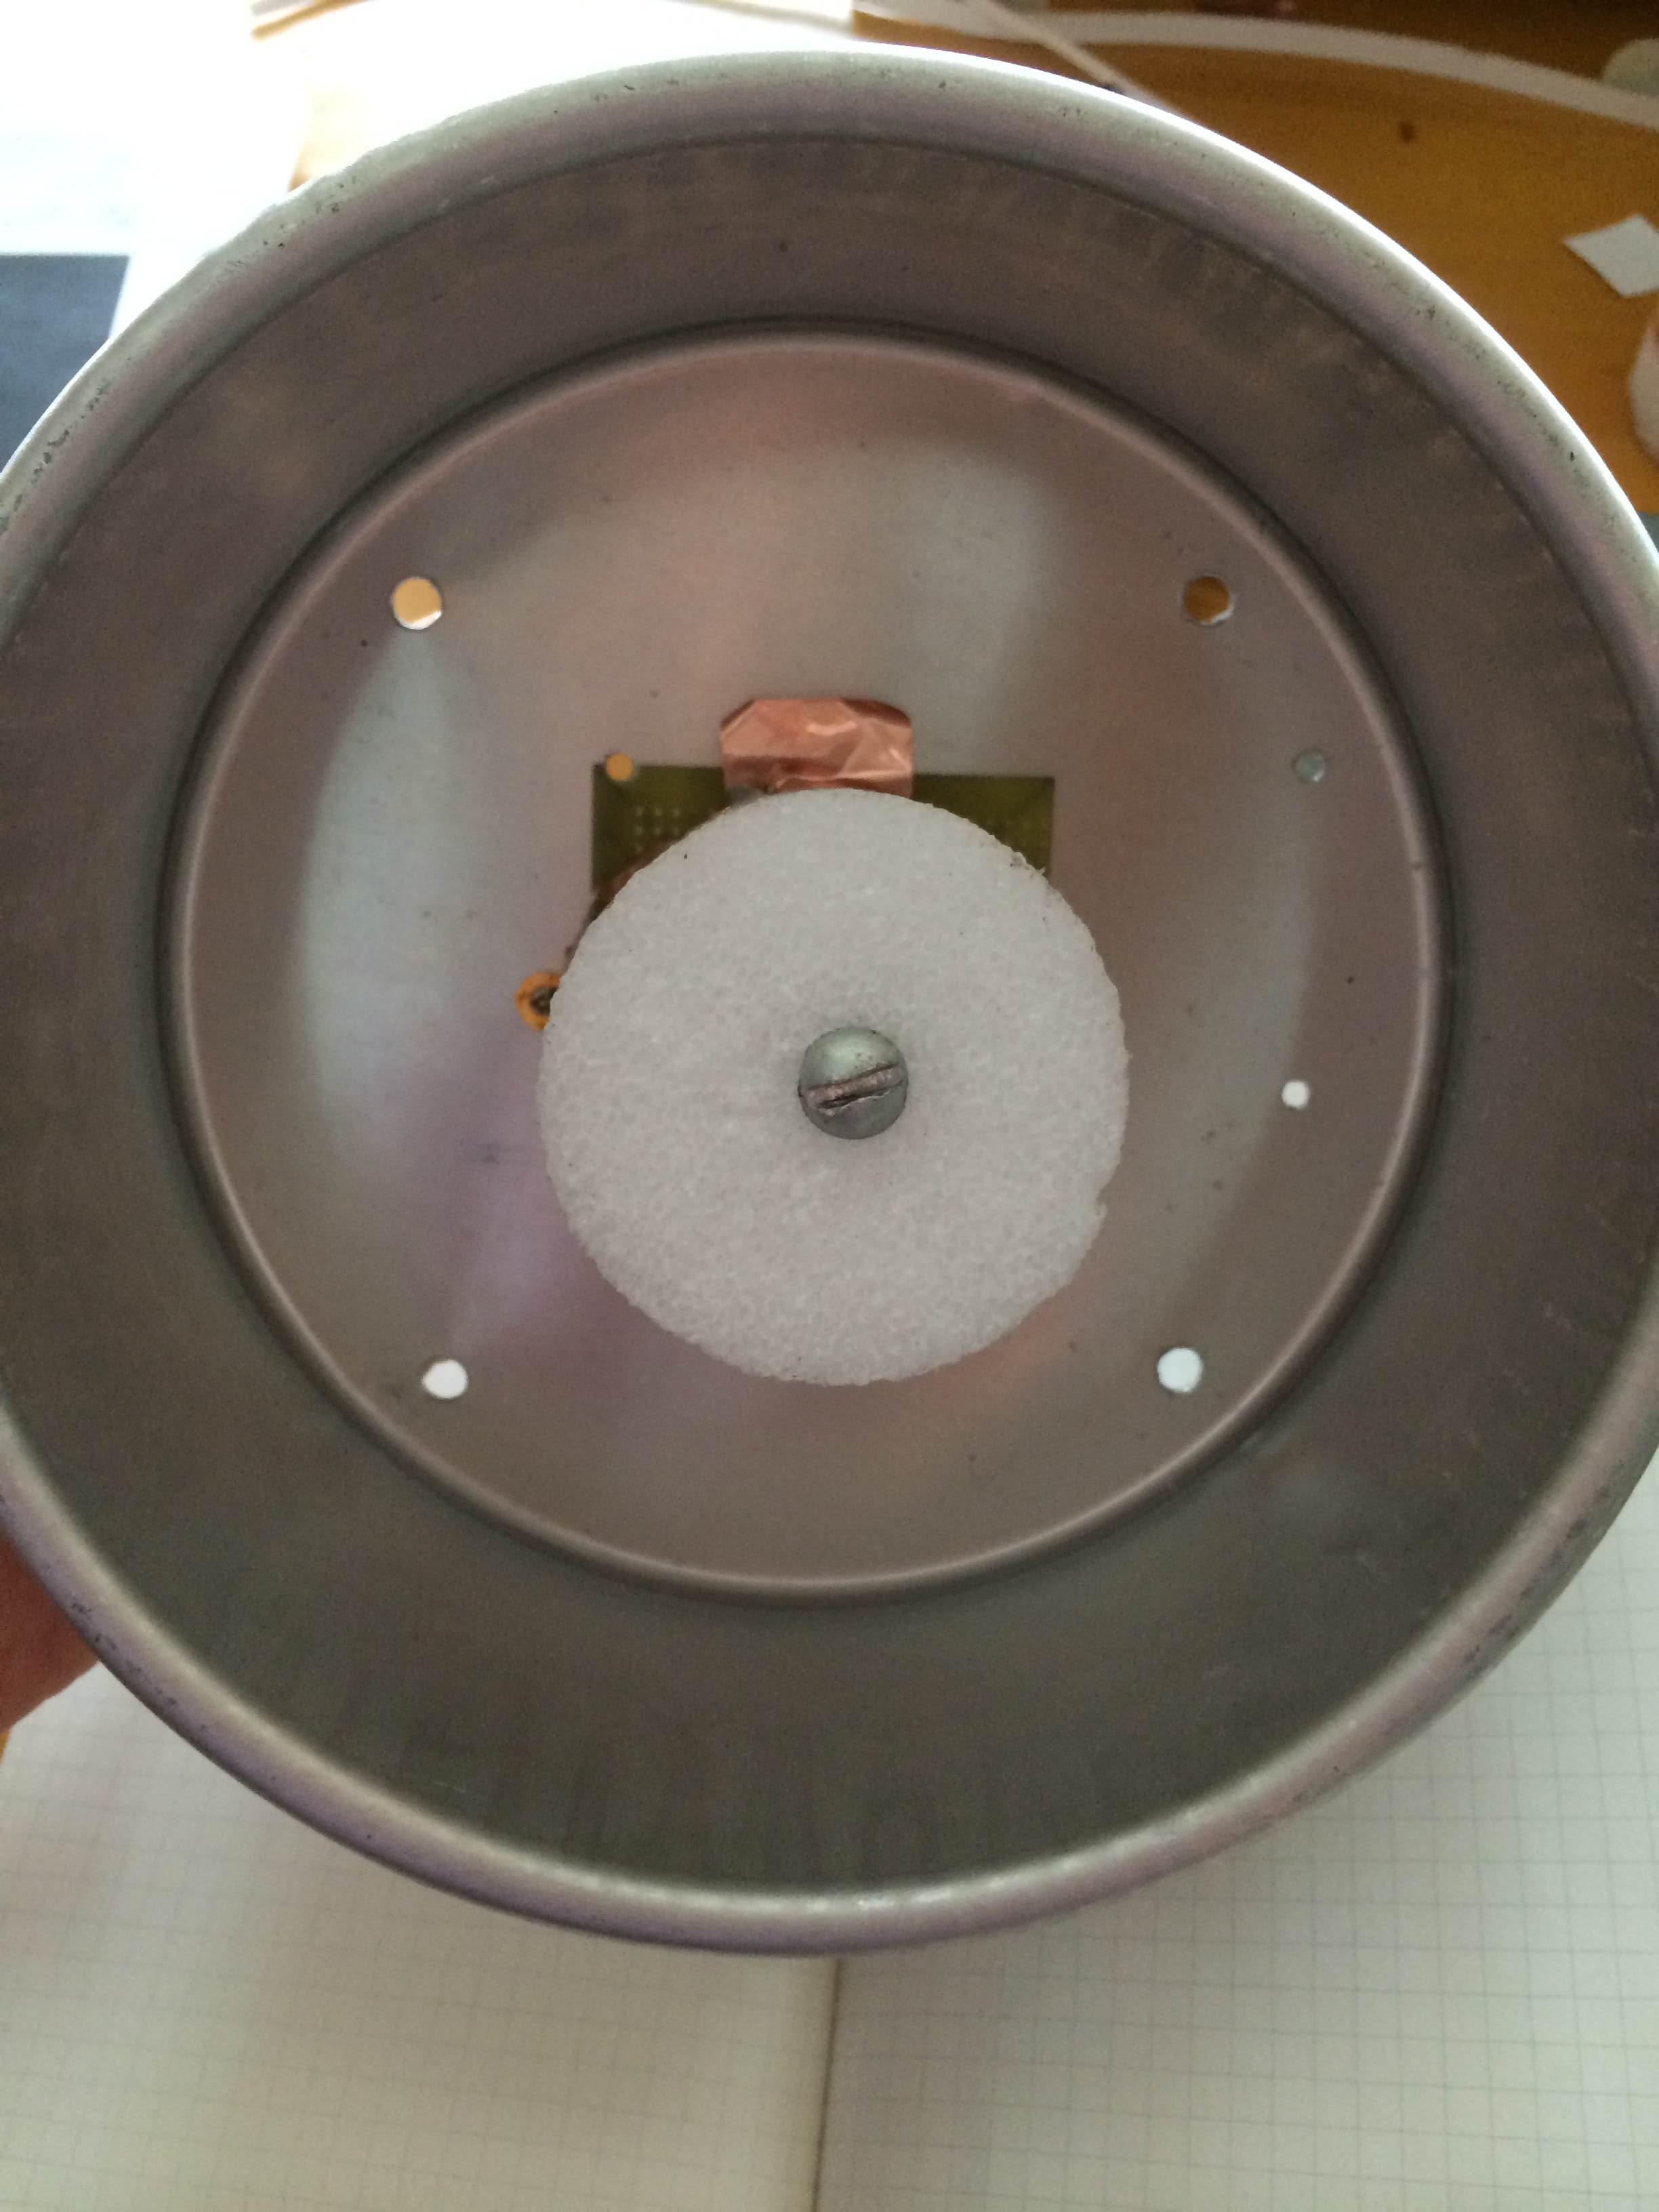
\includegraphics[scale=0.08]{feed/17.jpeg}
\end{center}

\begin{center}
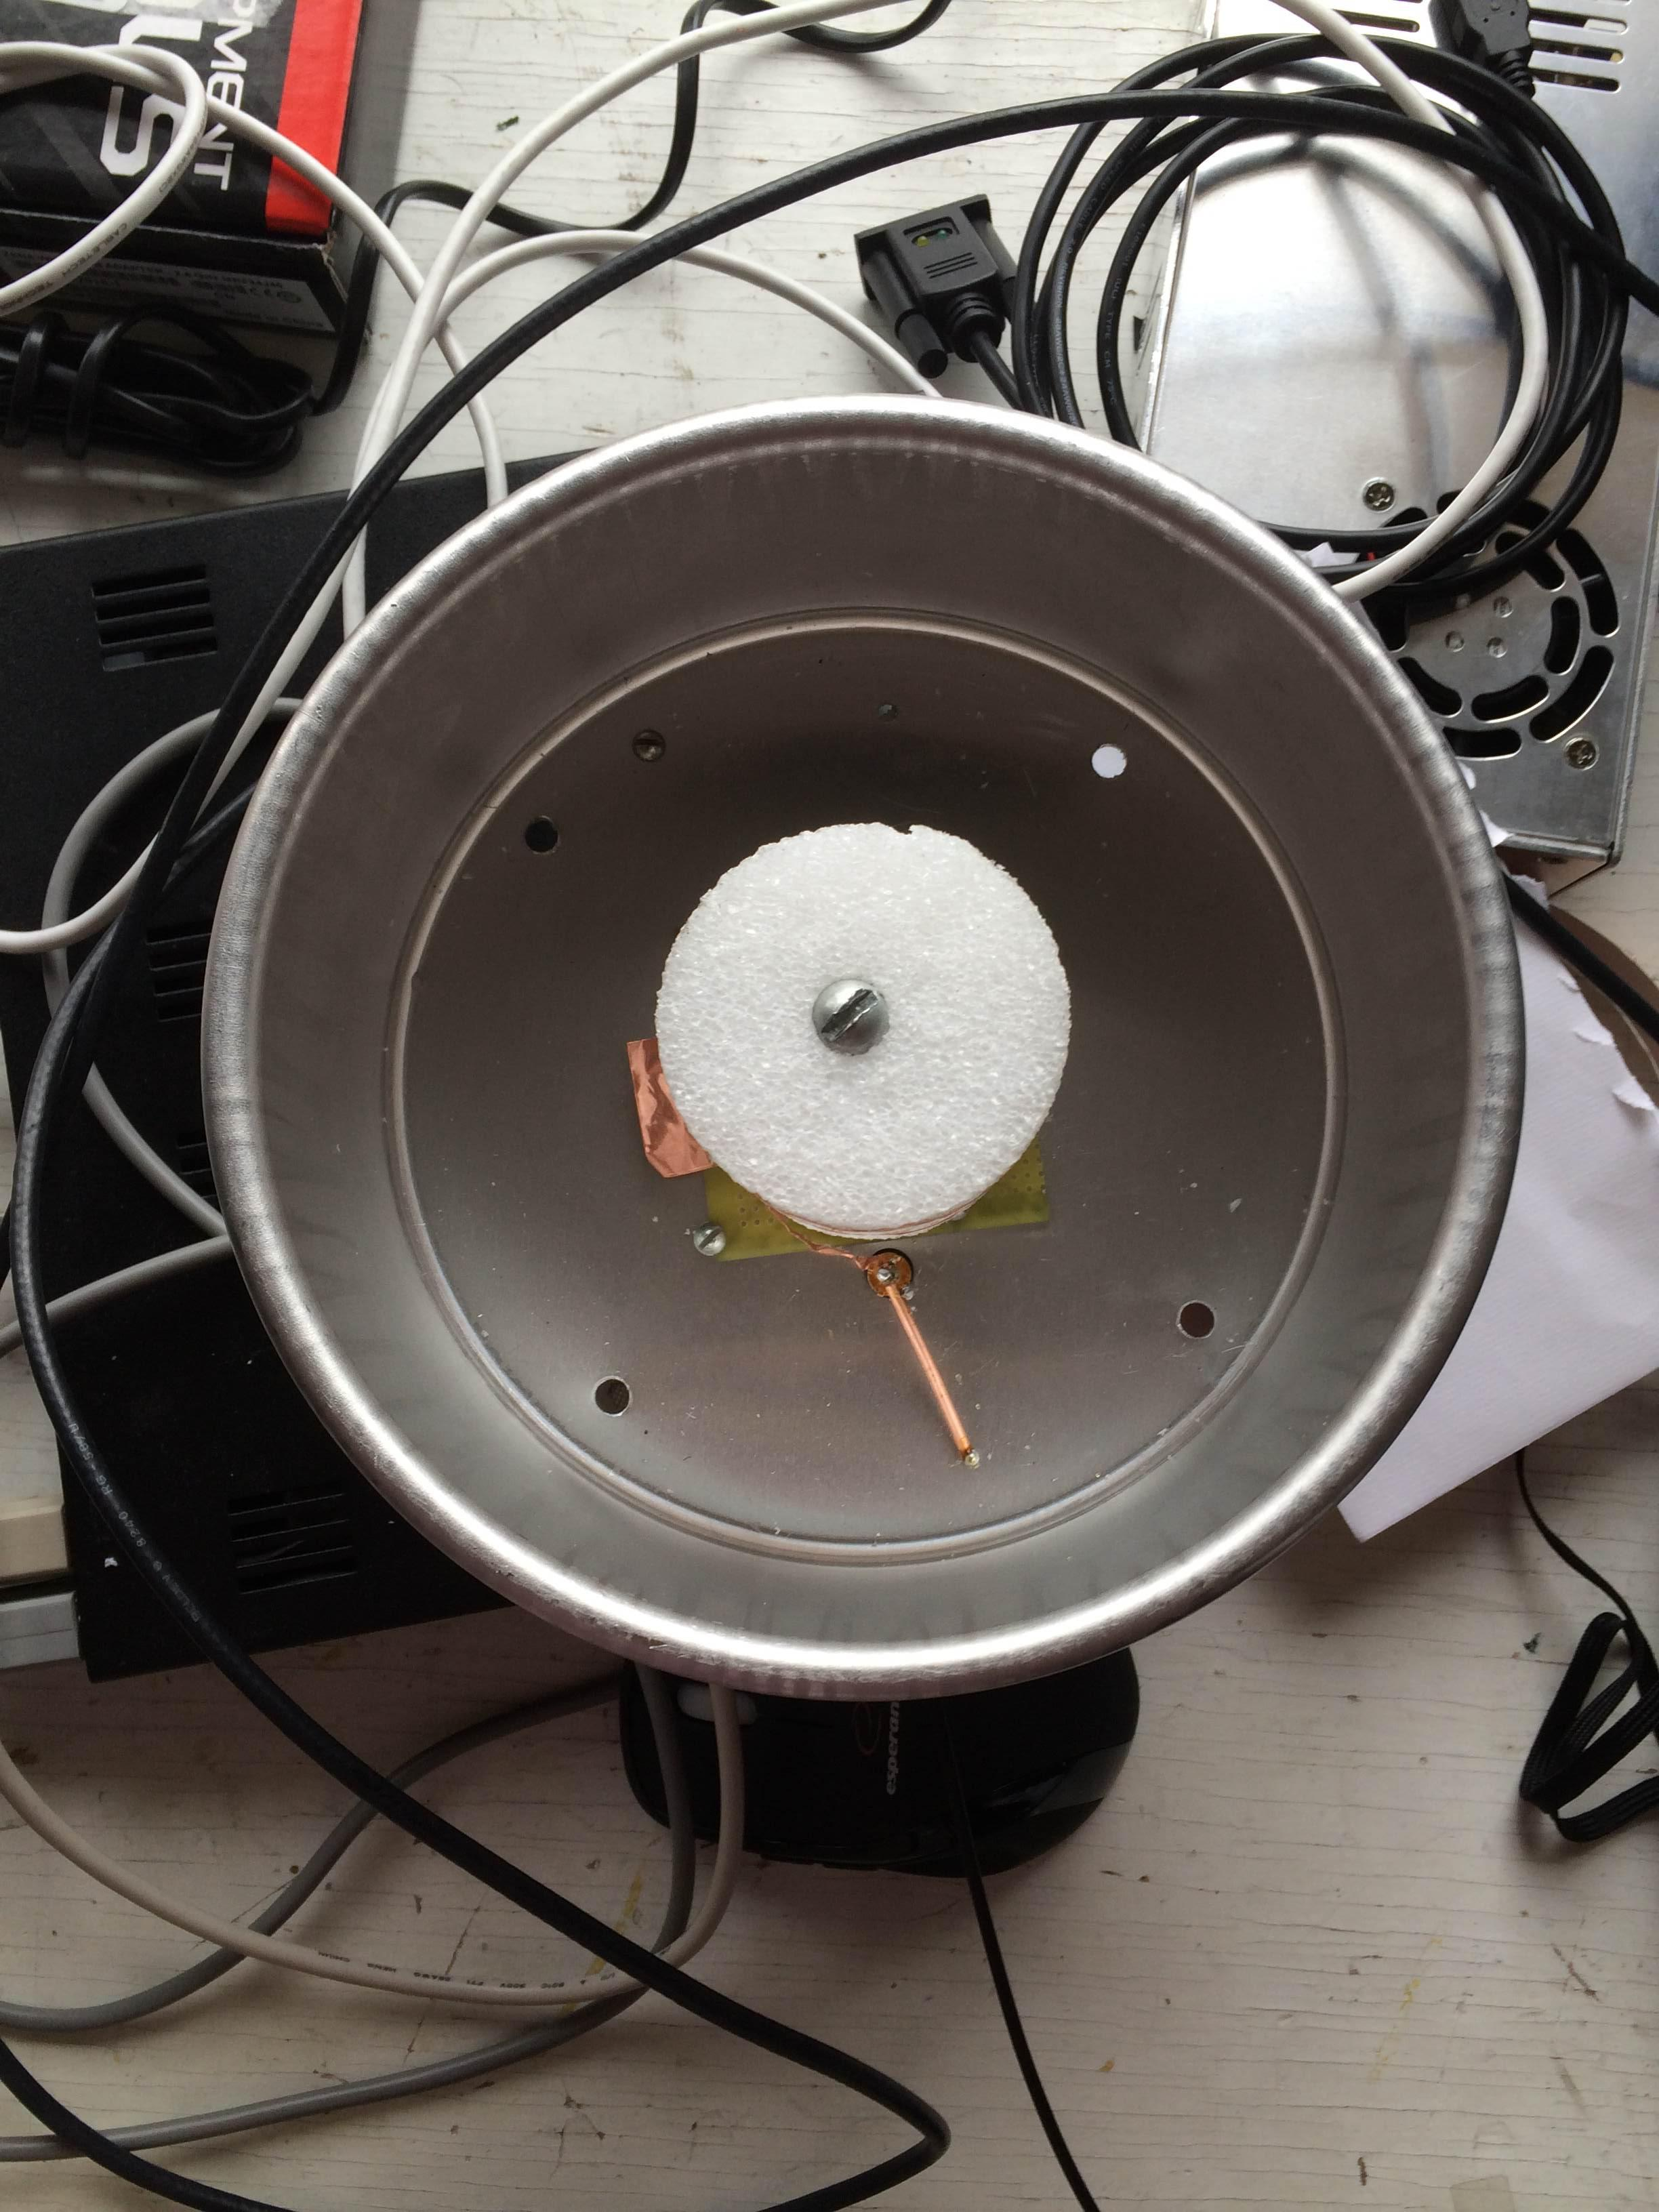
\includegraphics[scale=0.08]{feed/18.jpeg}
\end{center}

\begin{center}
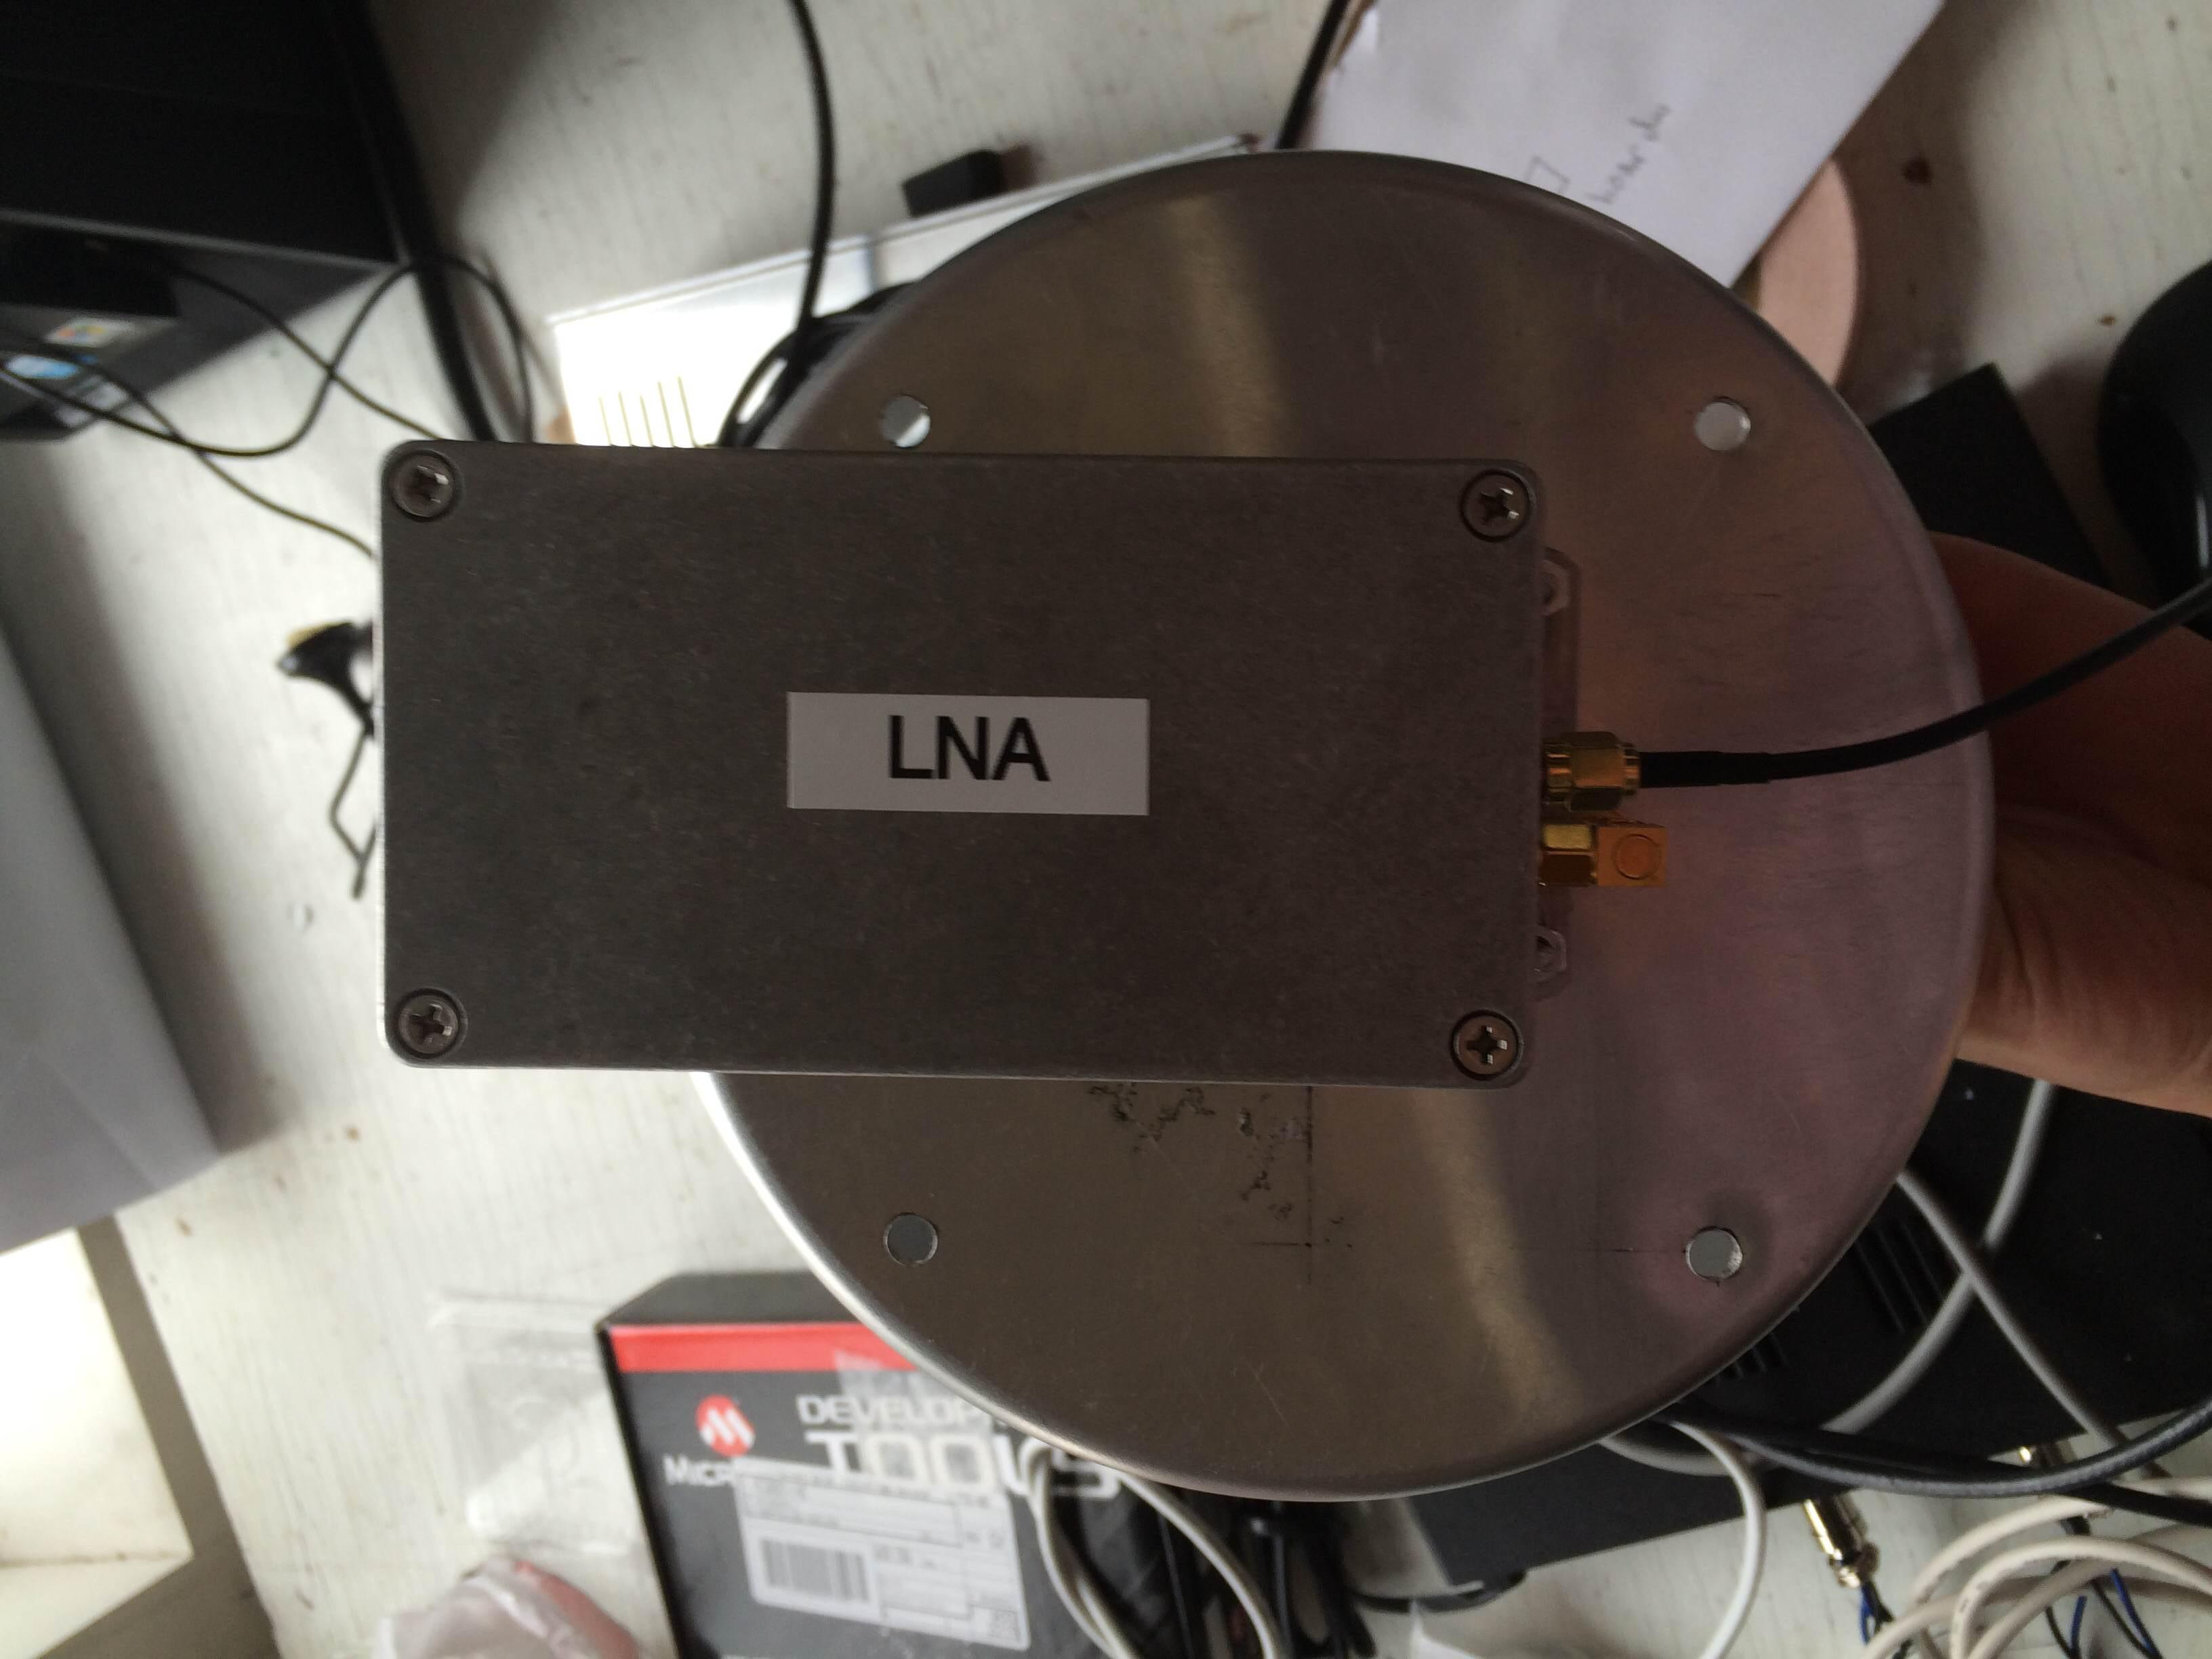
\includegraphics[scale=0.08]{feed/19.jpeg}
\end{center}

\begin{center}
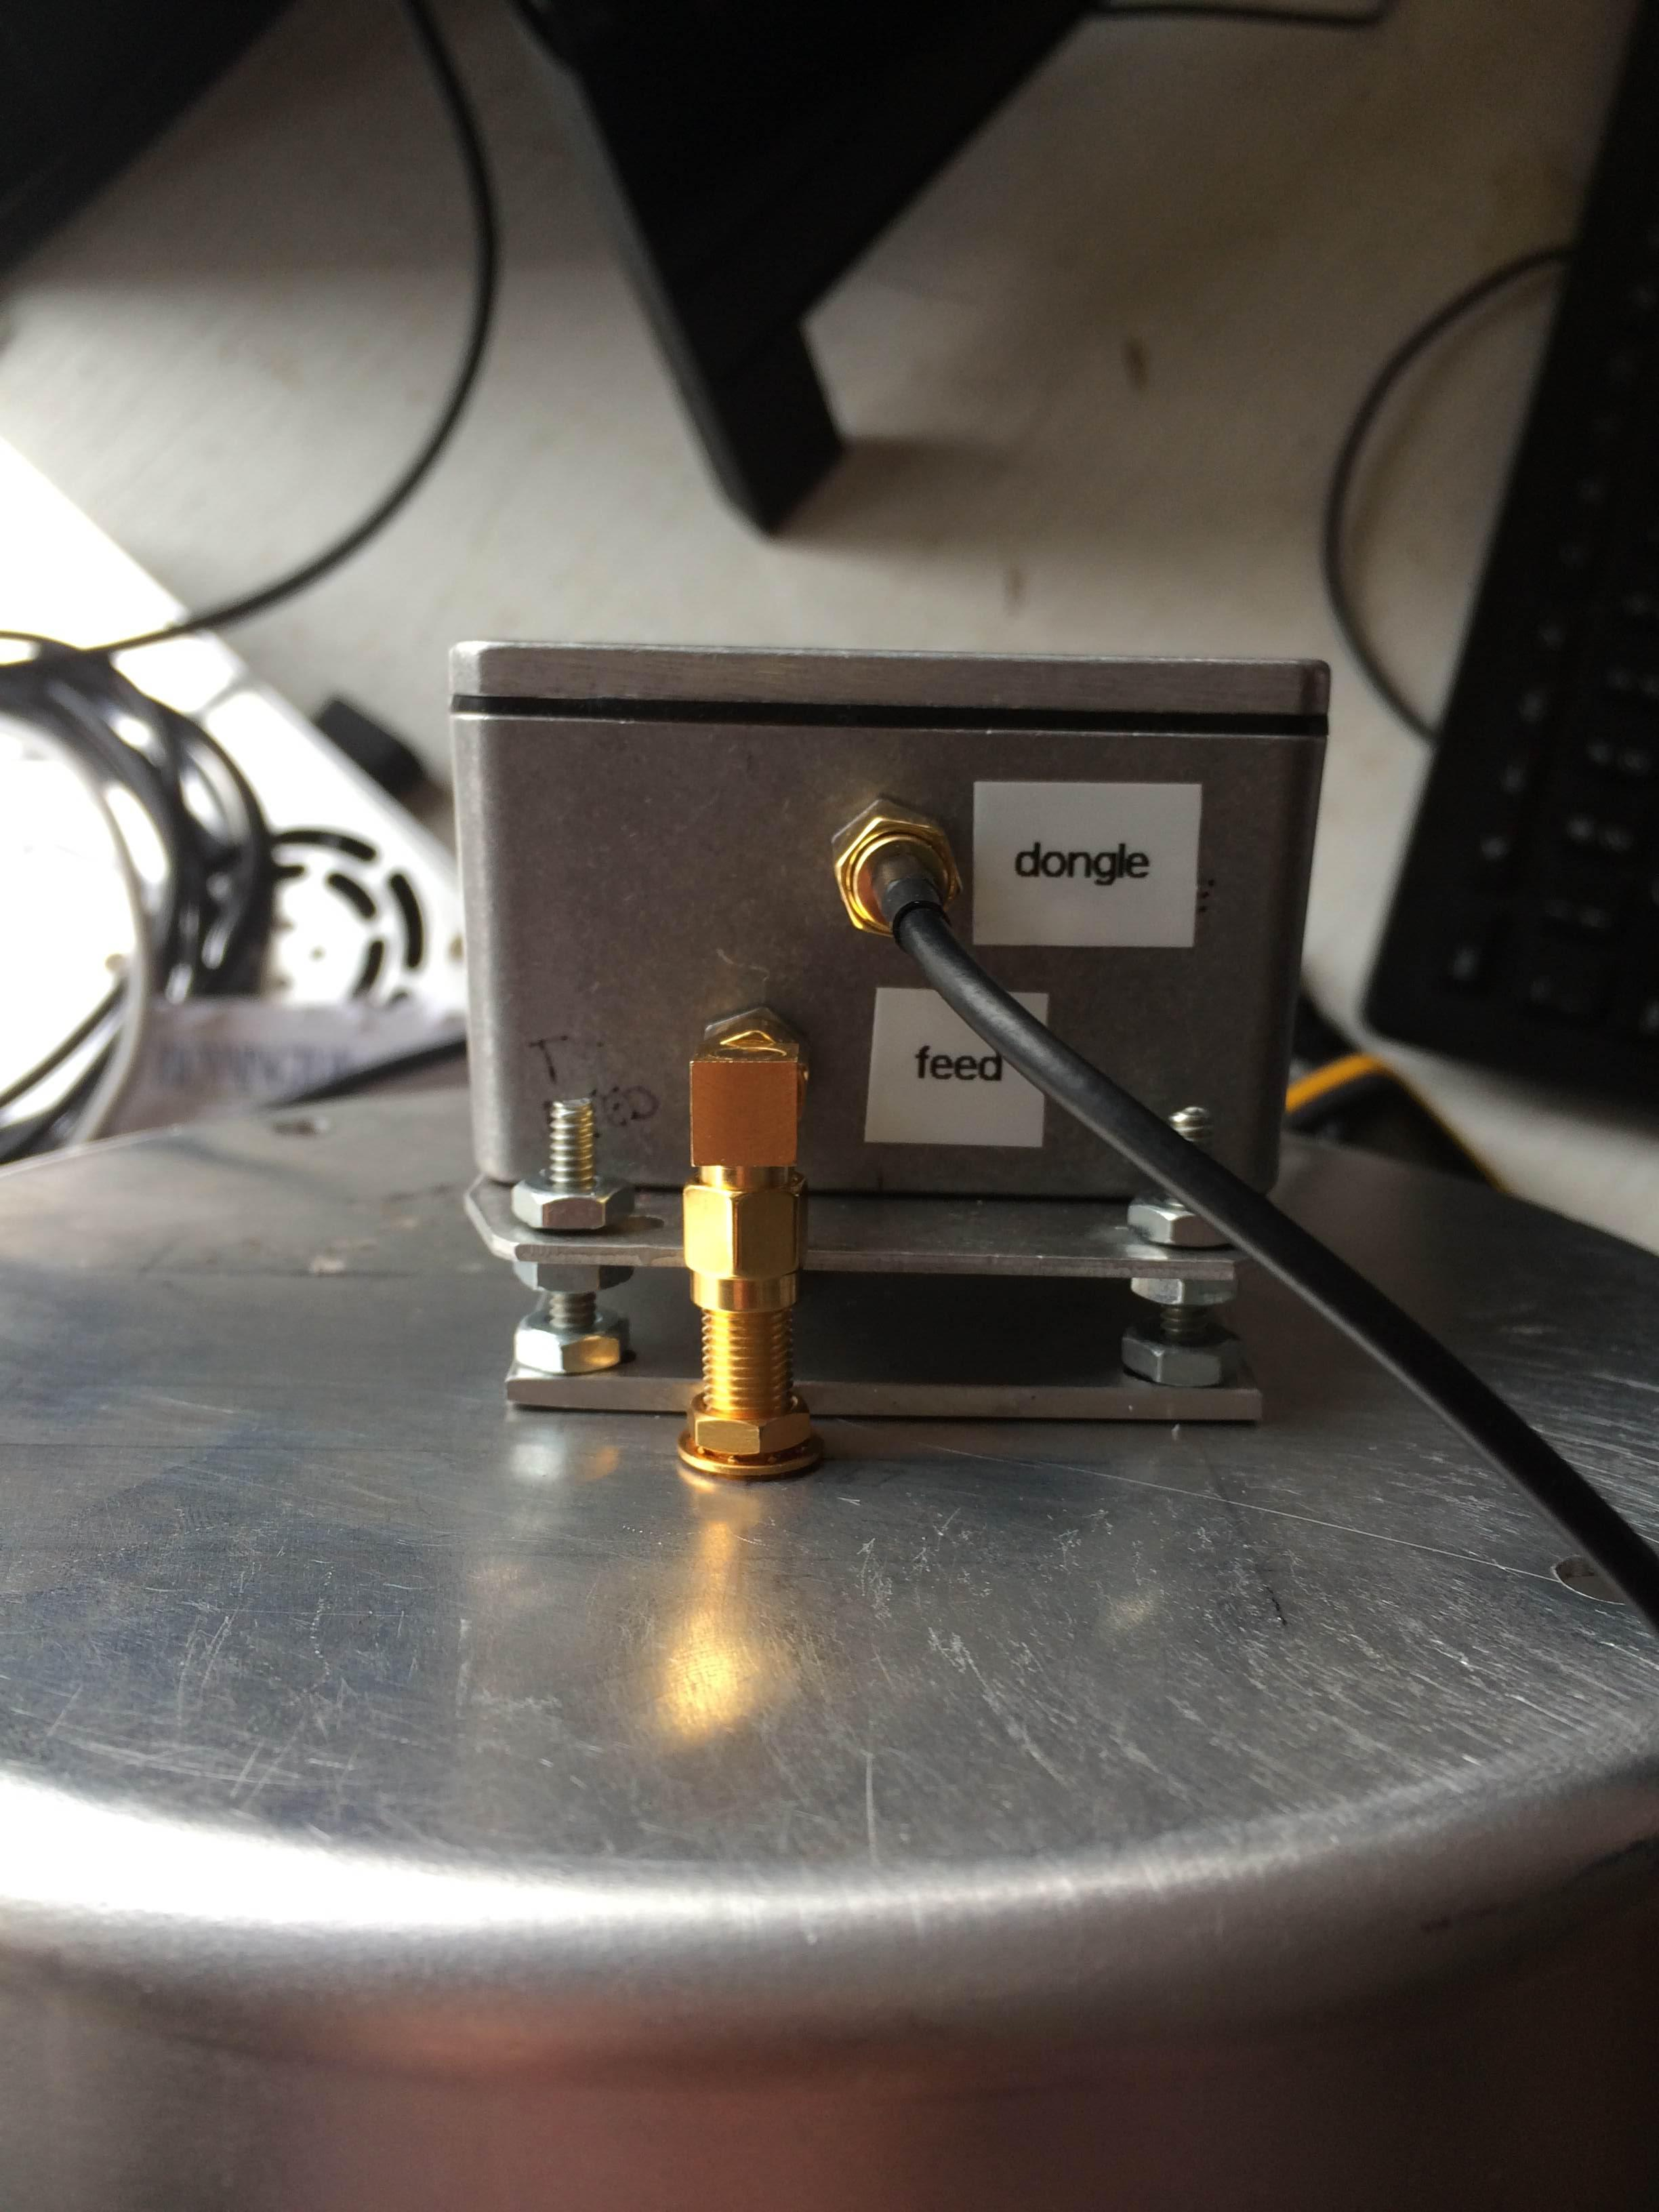
\includegraphics[scale=0.08]{feed/20.jpeg}
\end{center}





%%%%%%%%%%%%%%%%%%%%%%%%%%%%%%%%%%%%%%%%

\subsection{Roof Mount}

\begin{center}
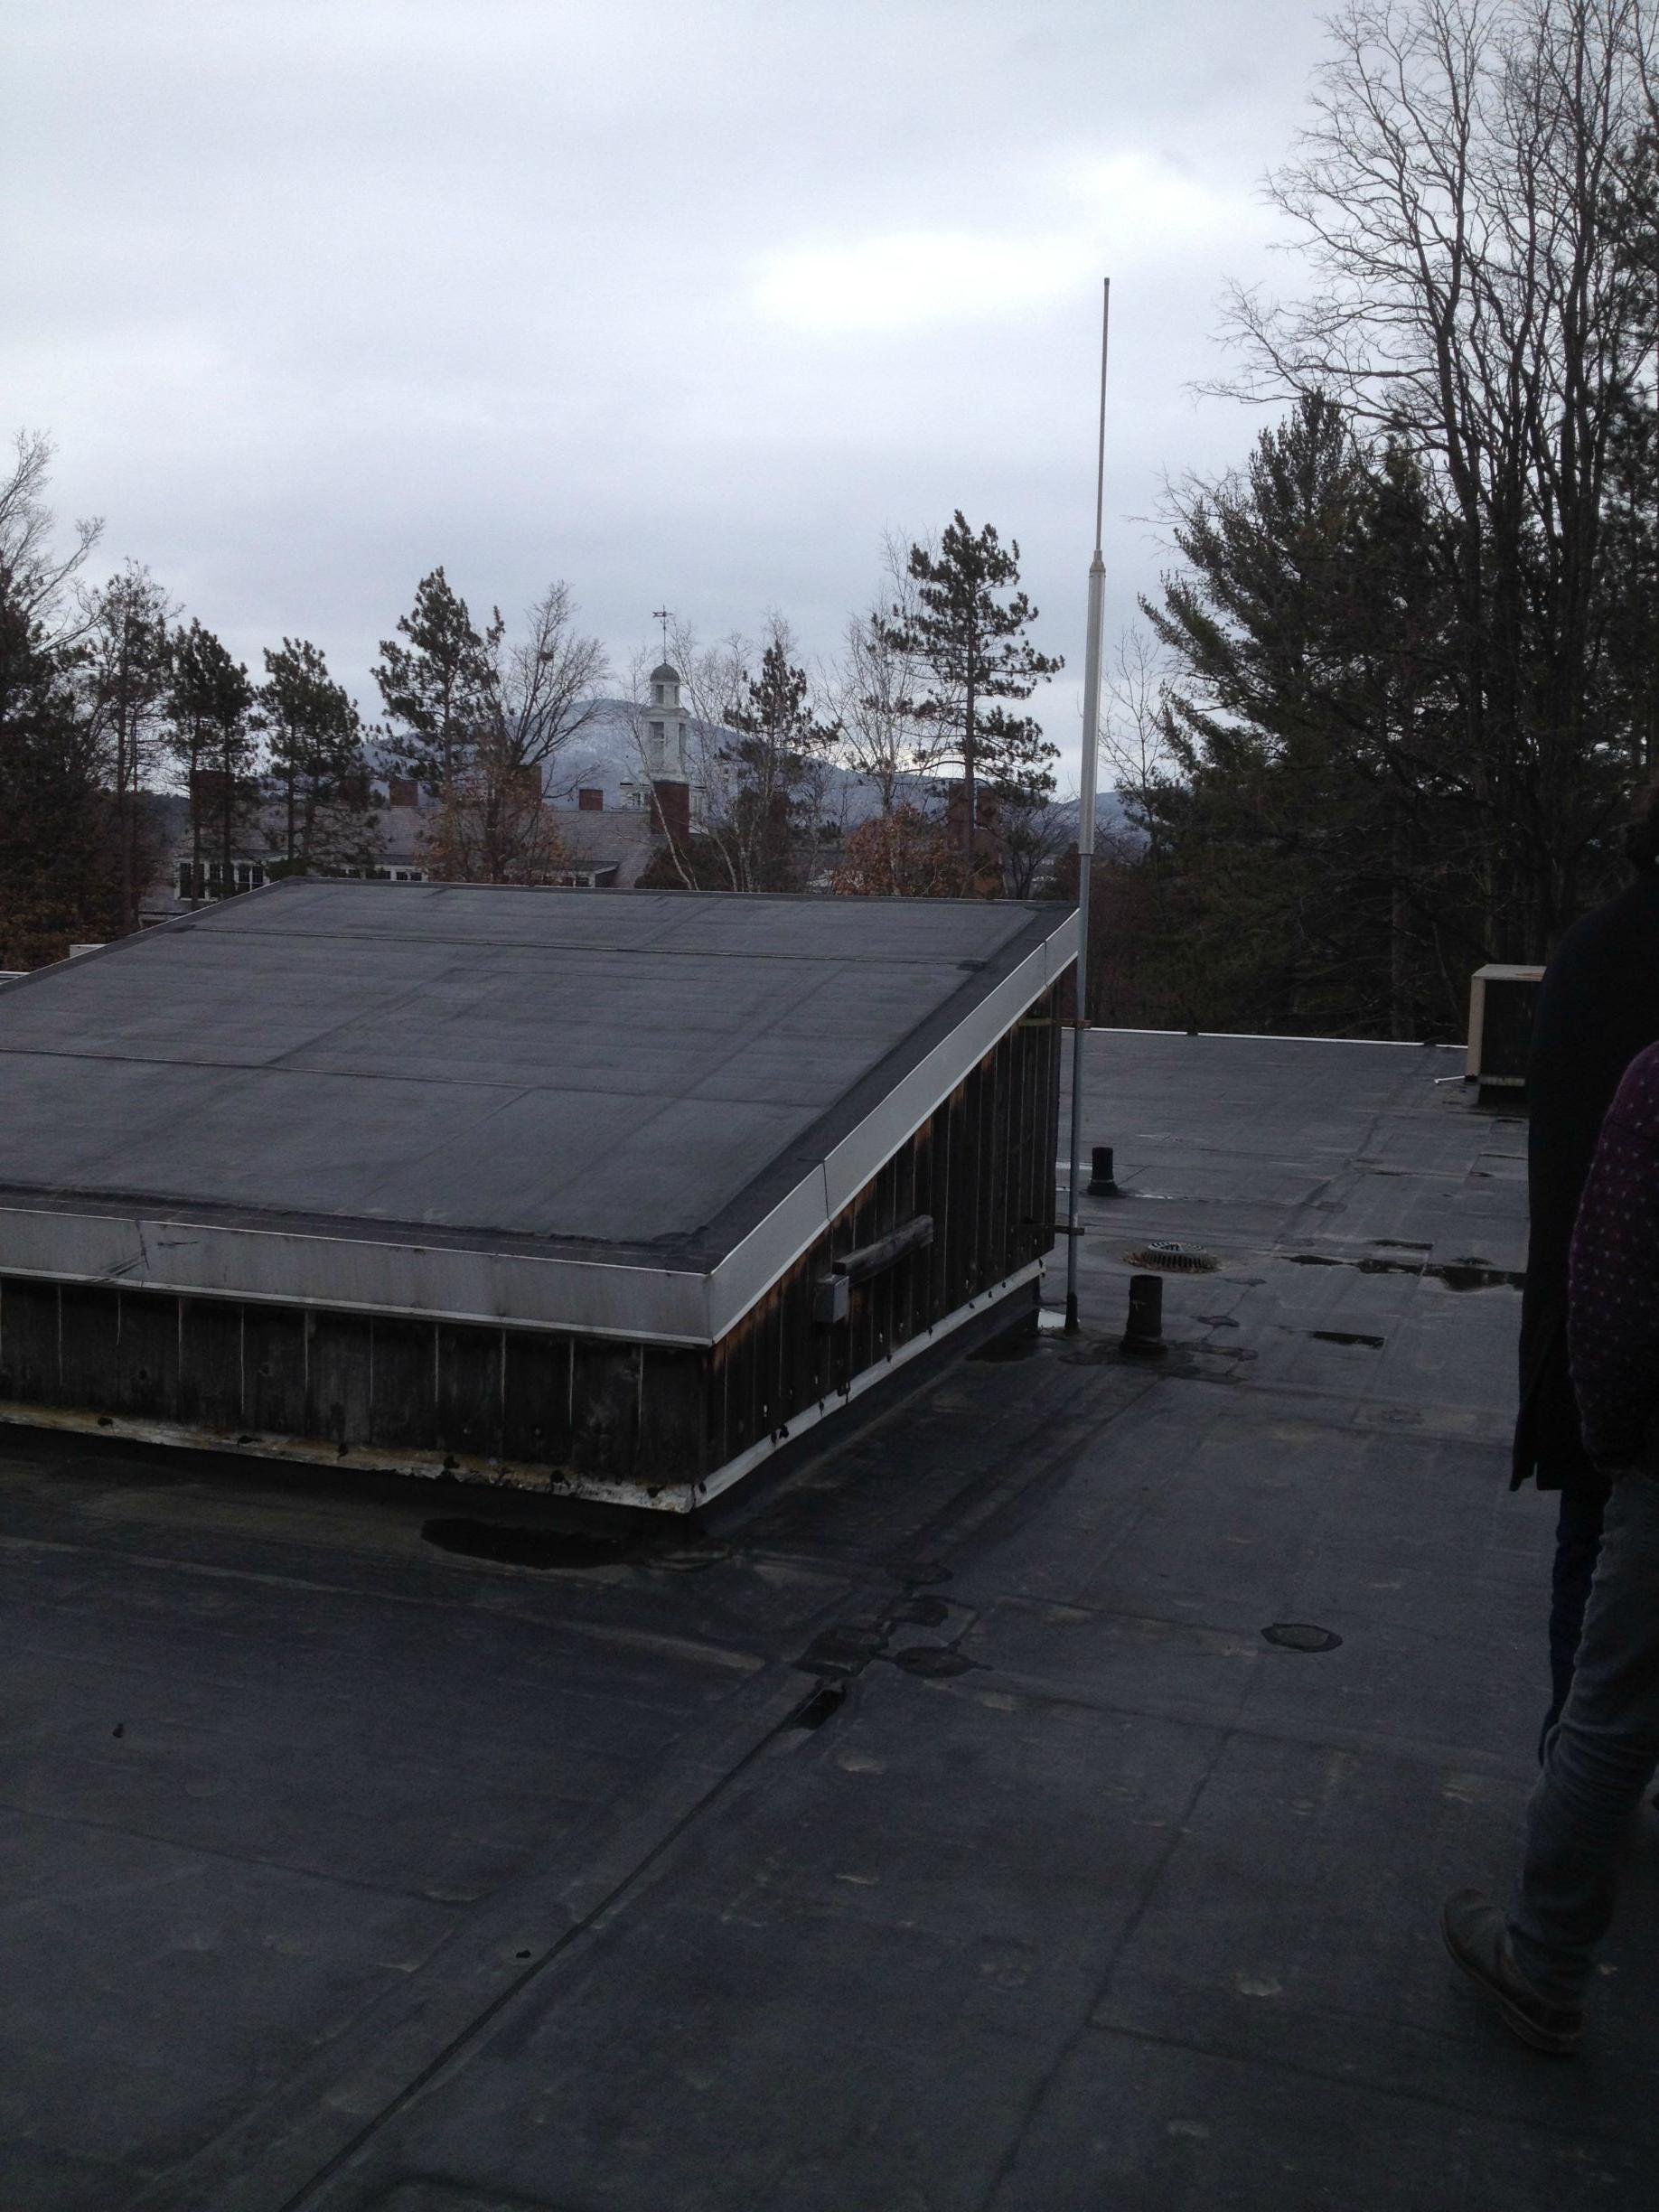
\includegraphics[scale=0.12]{roofmount/00.jpeg}
\end{center}

We used scrap metal to make our dish mount so we had to start by cleaning up the pieces of metal we were going to use and make them the right size.

We plasma cut a 1.5' x 3' rectangle of 5 gauge steel (about 3/16" thick, it later turned out this is to thin) and cleaned up the edges with a grinder.

\begin{center}
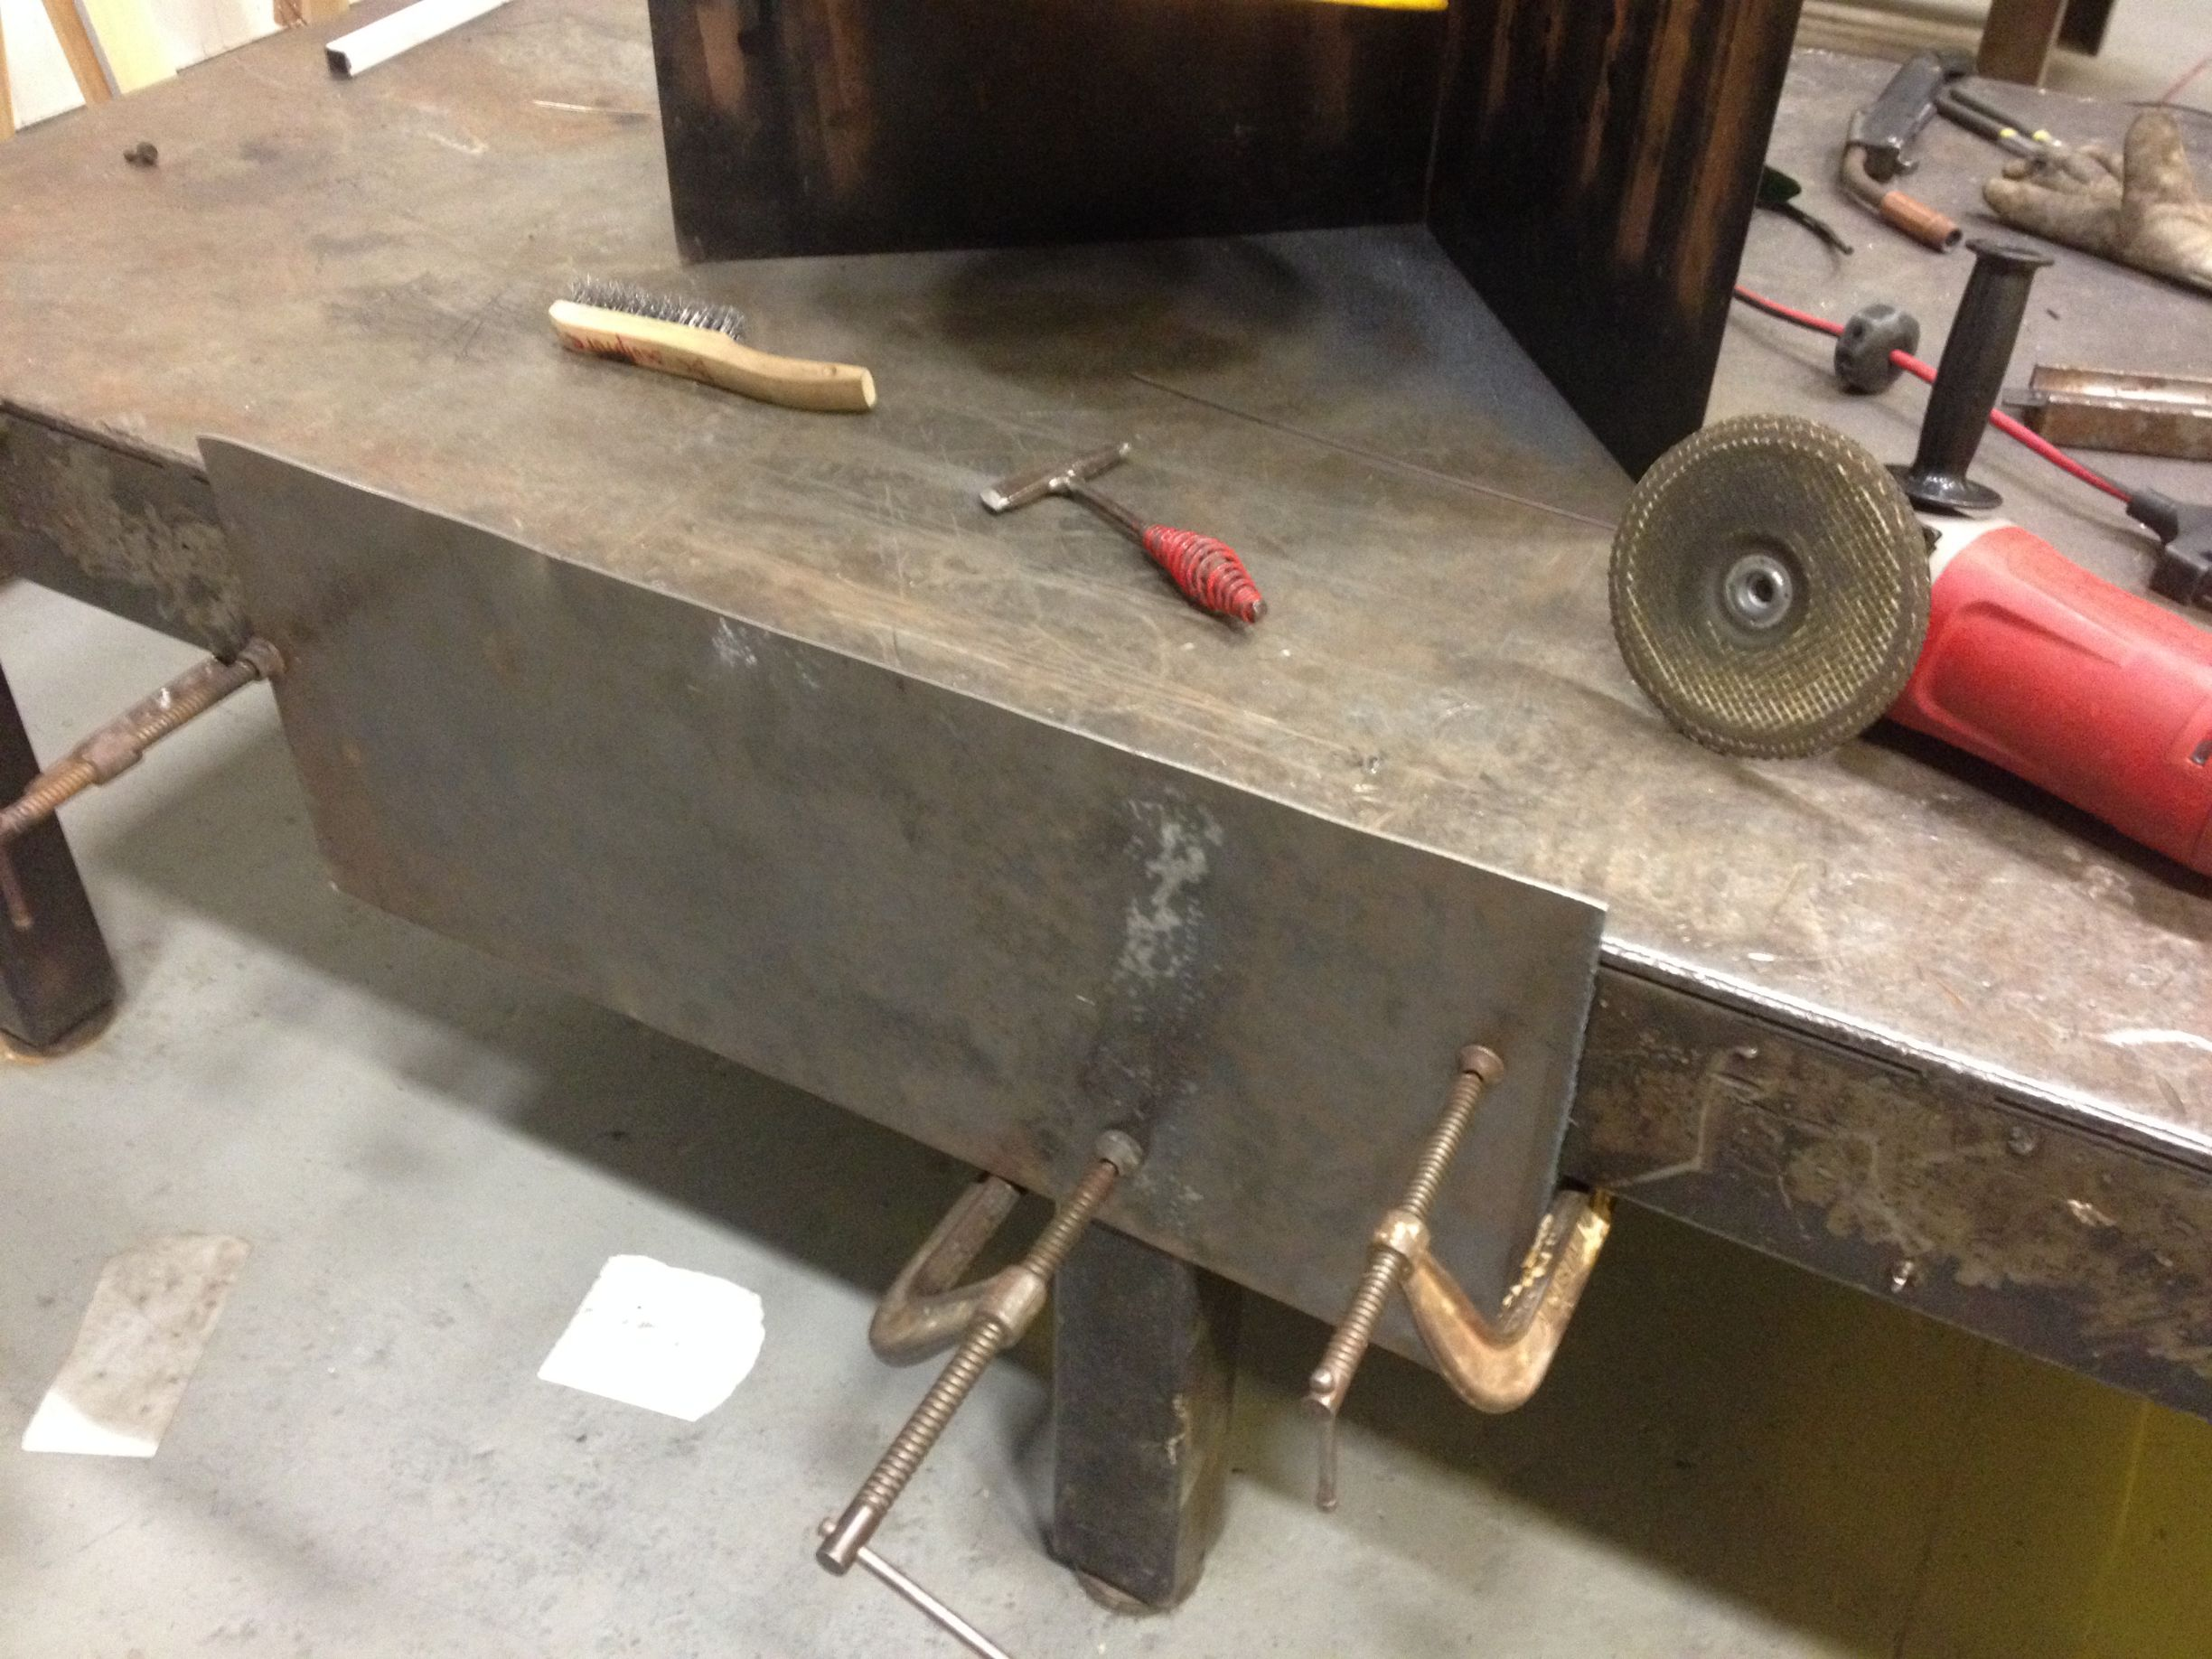
\includegraphics[scale=0.12]{roofmount/01.jpeg}
\end{center}

\begin{center}
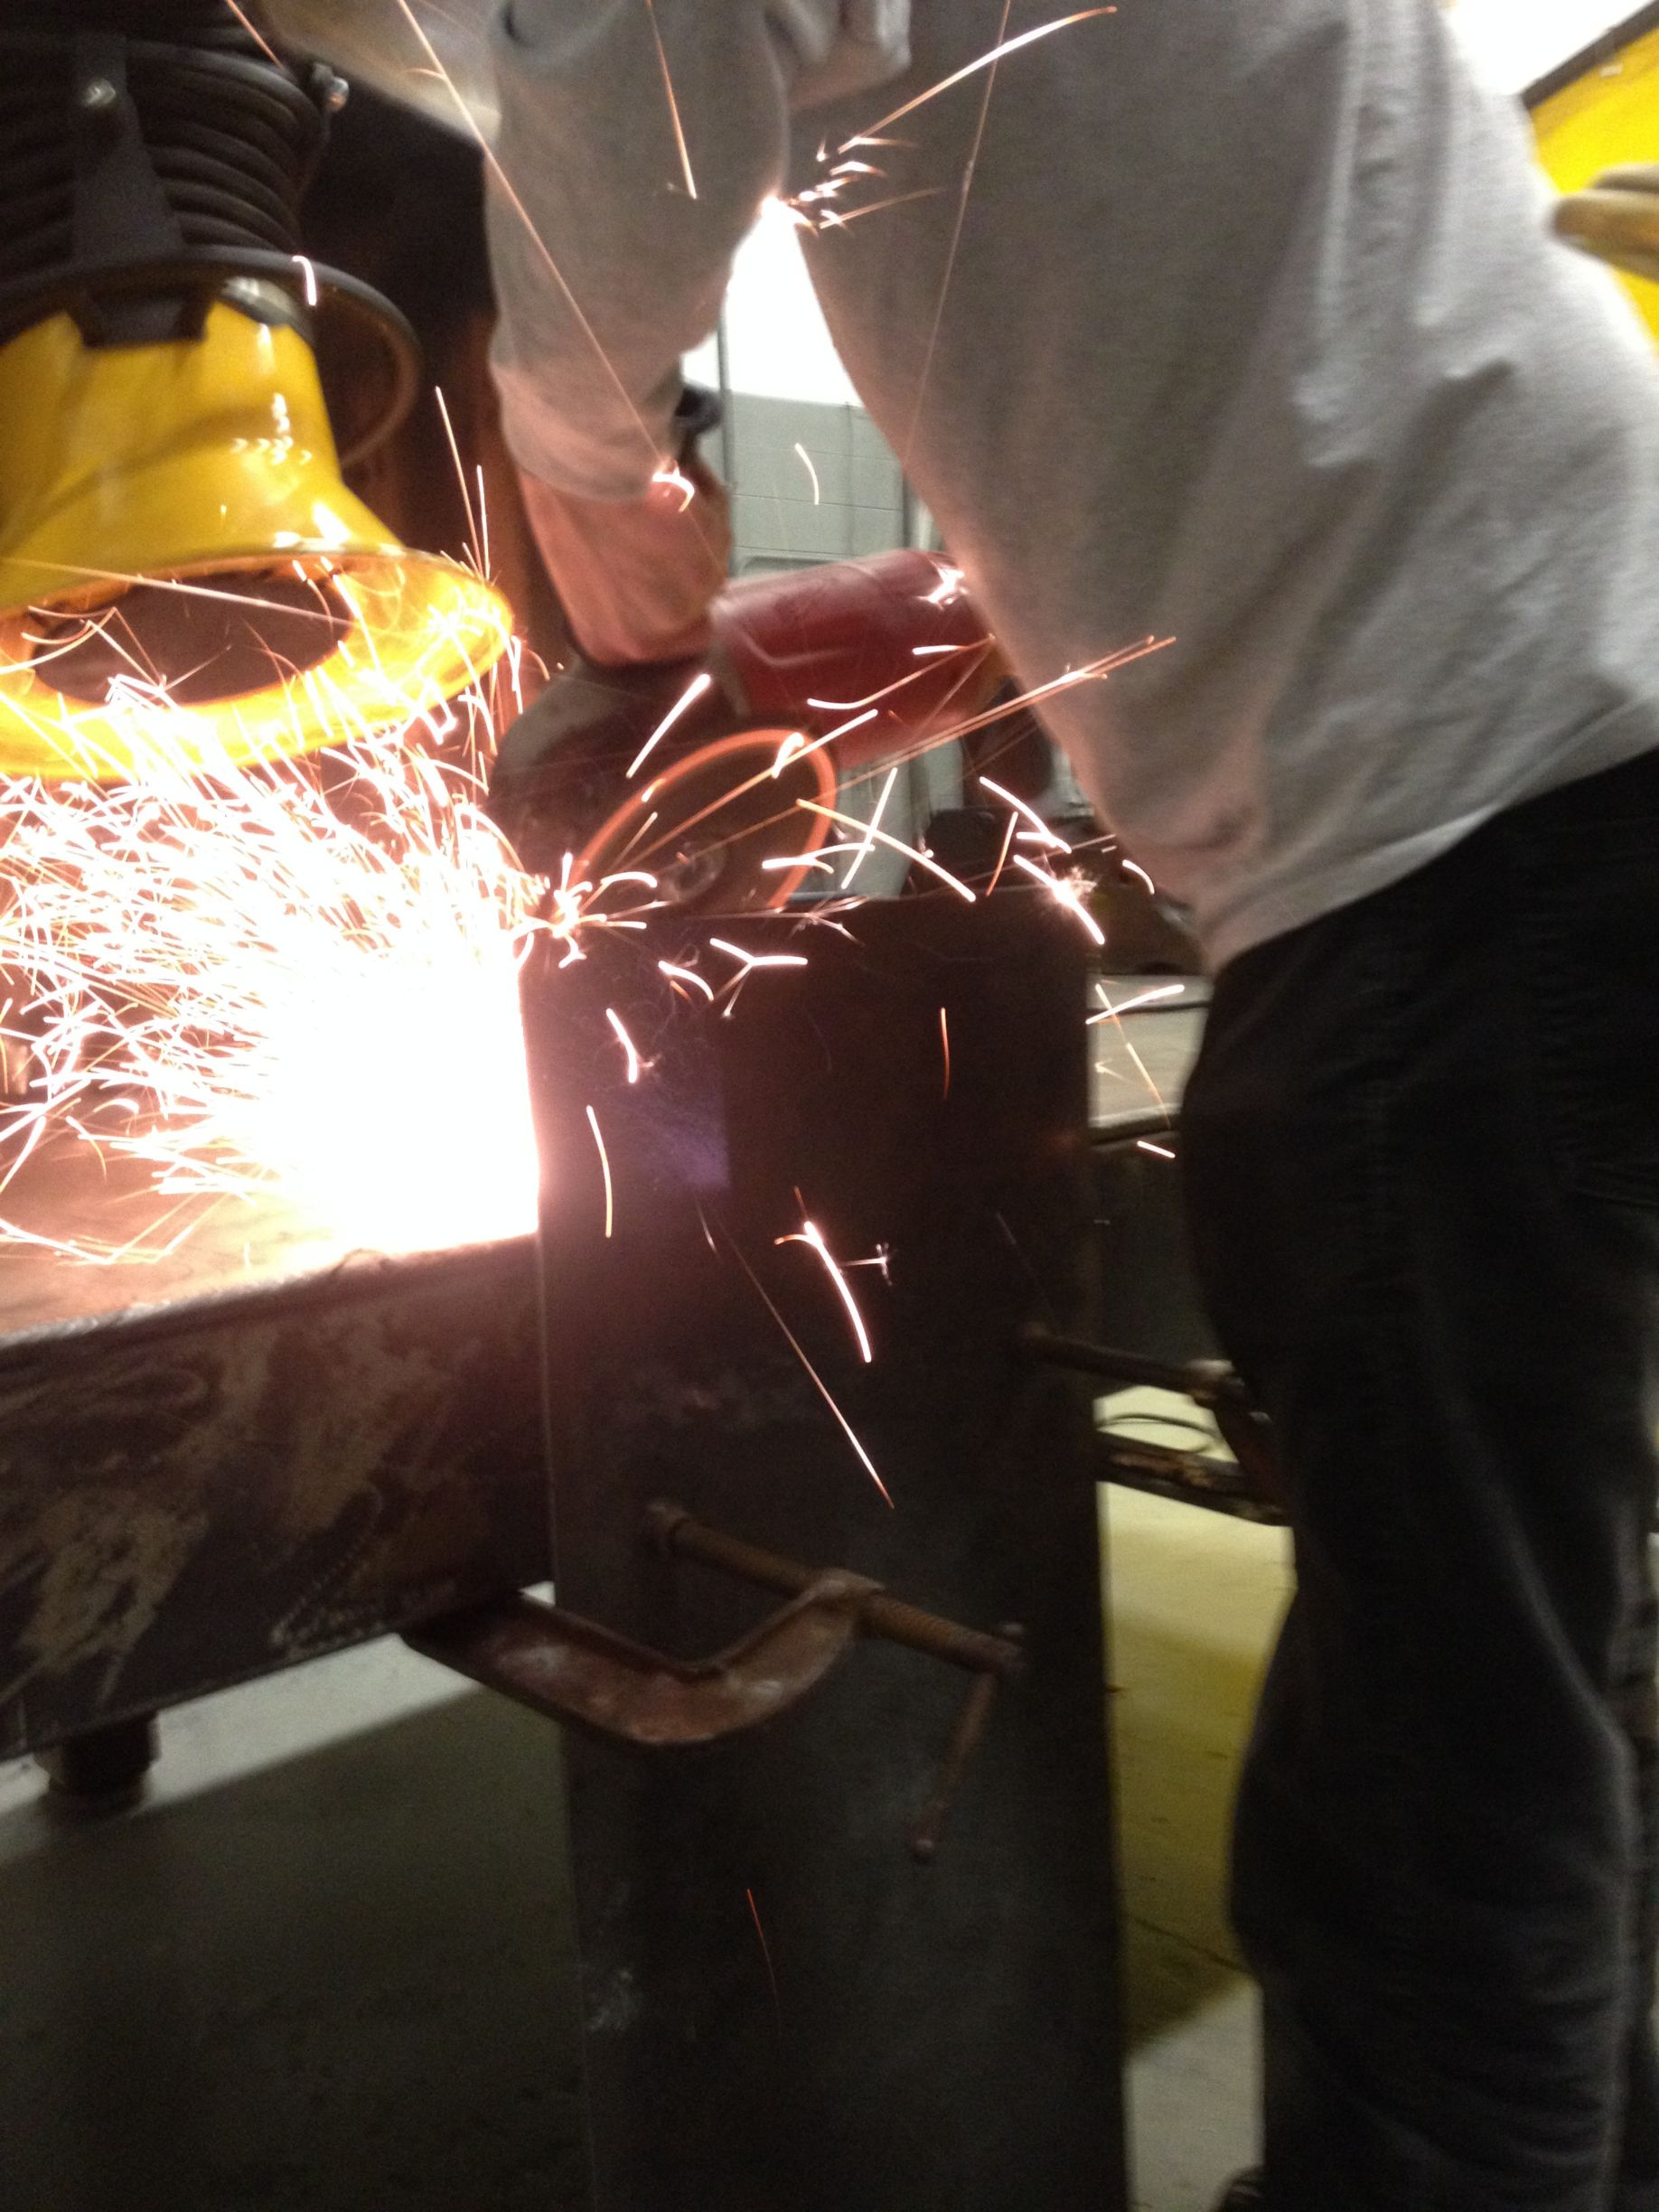
\includegraphics[scale=0.12]{roofmount/02.jpeg}
\end{center}


We cut an 11.5' length of 2.5" (exterior diameter) pipe and cleaned in using a steel brush head on a grinder.

\begin{center}
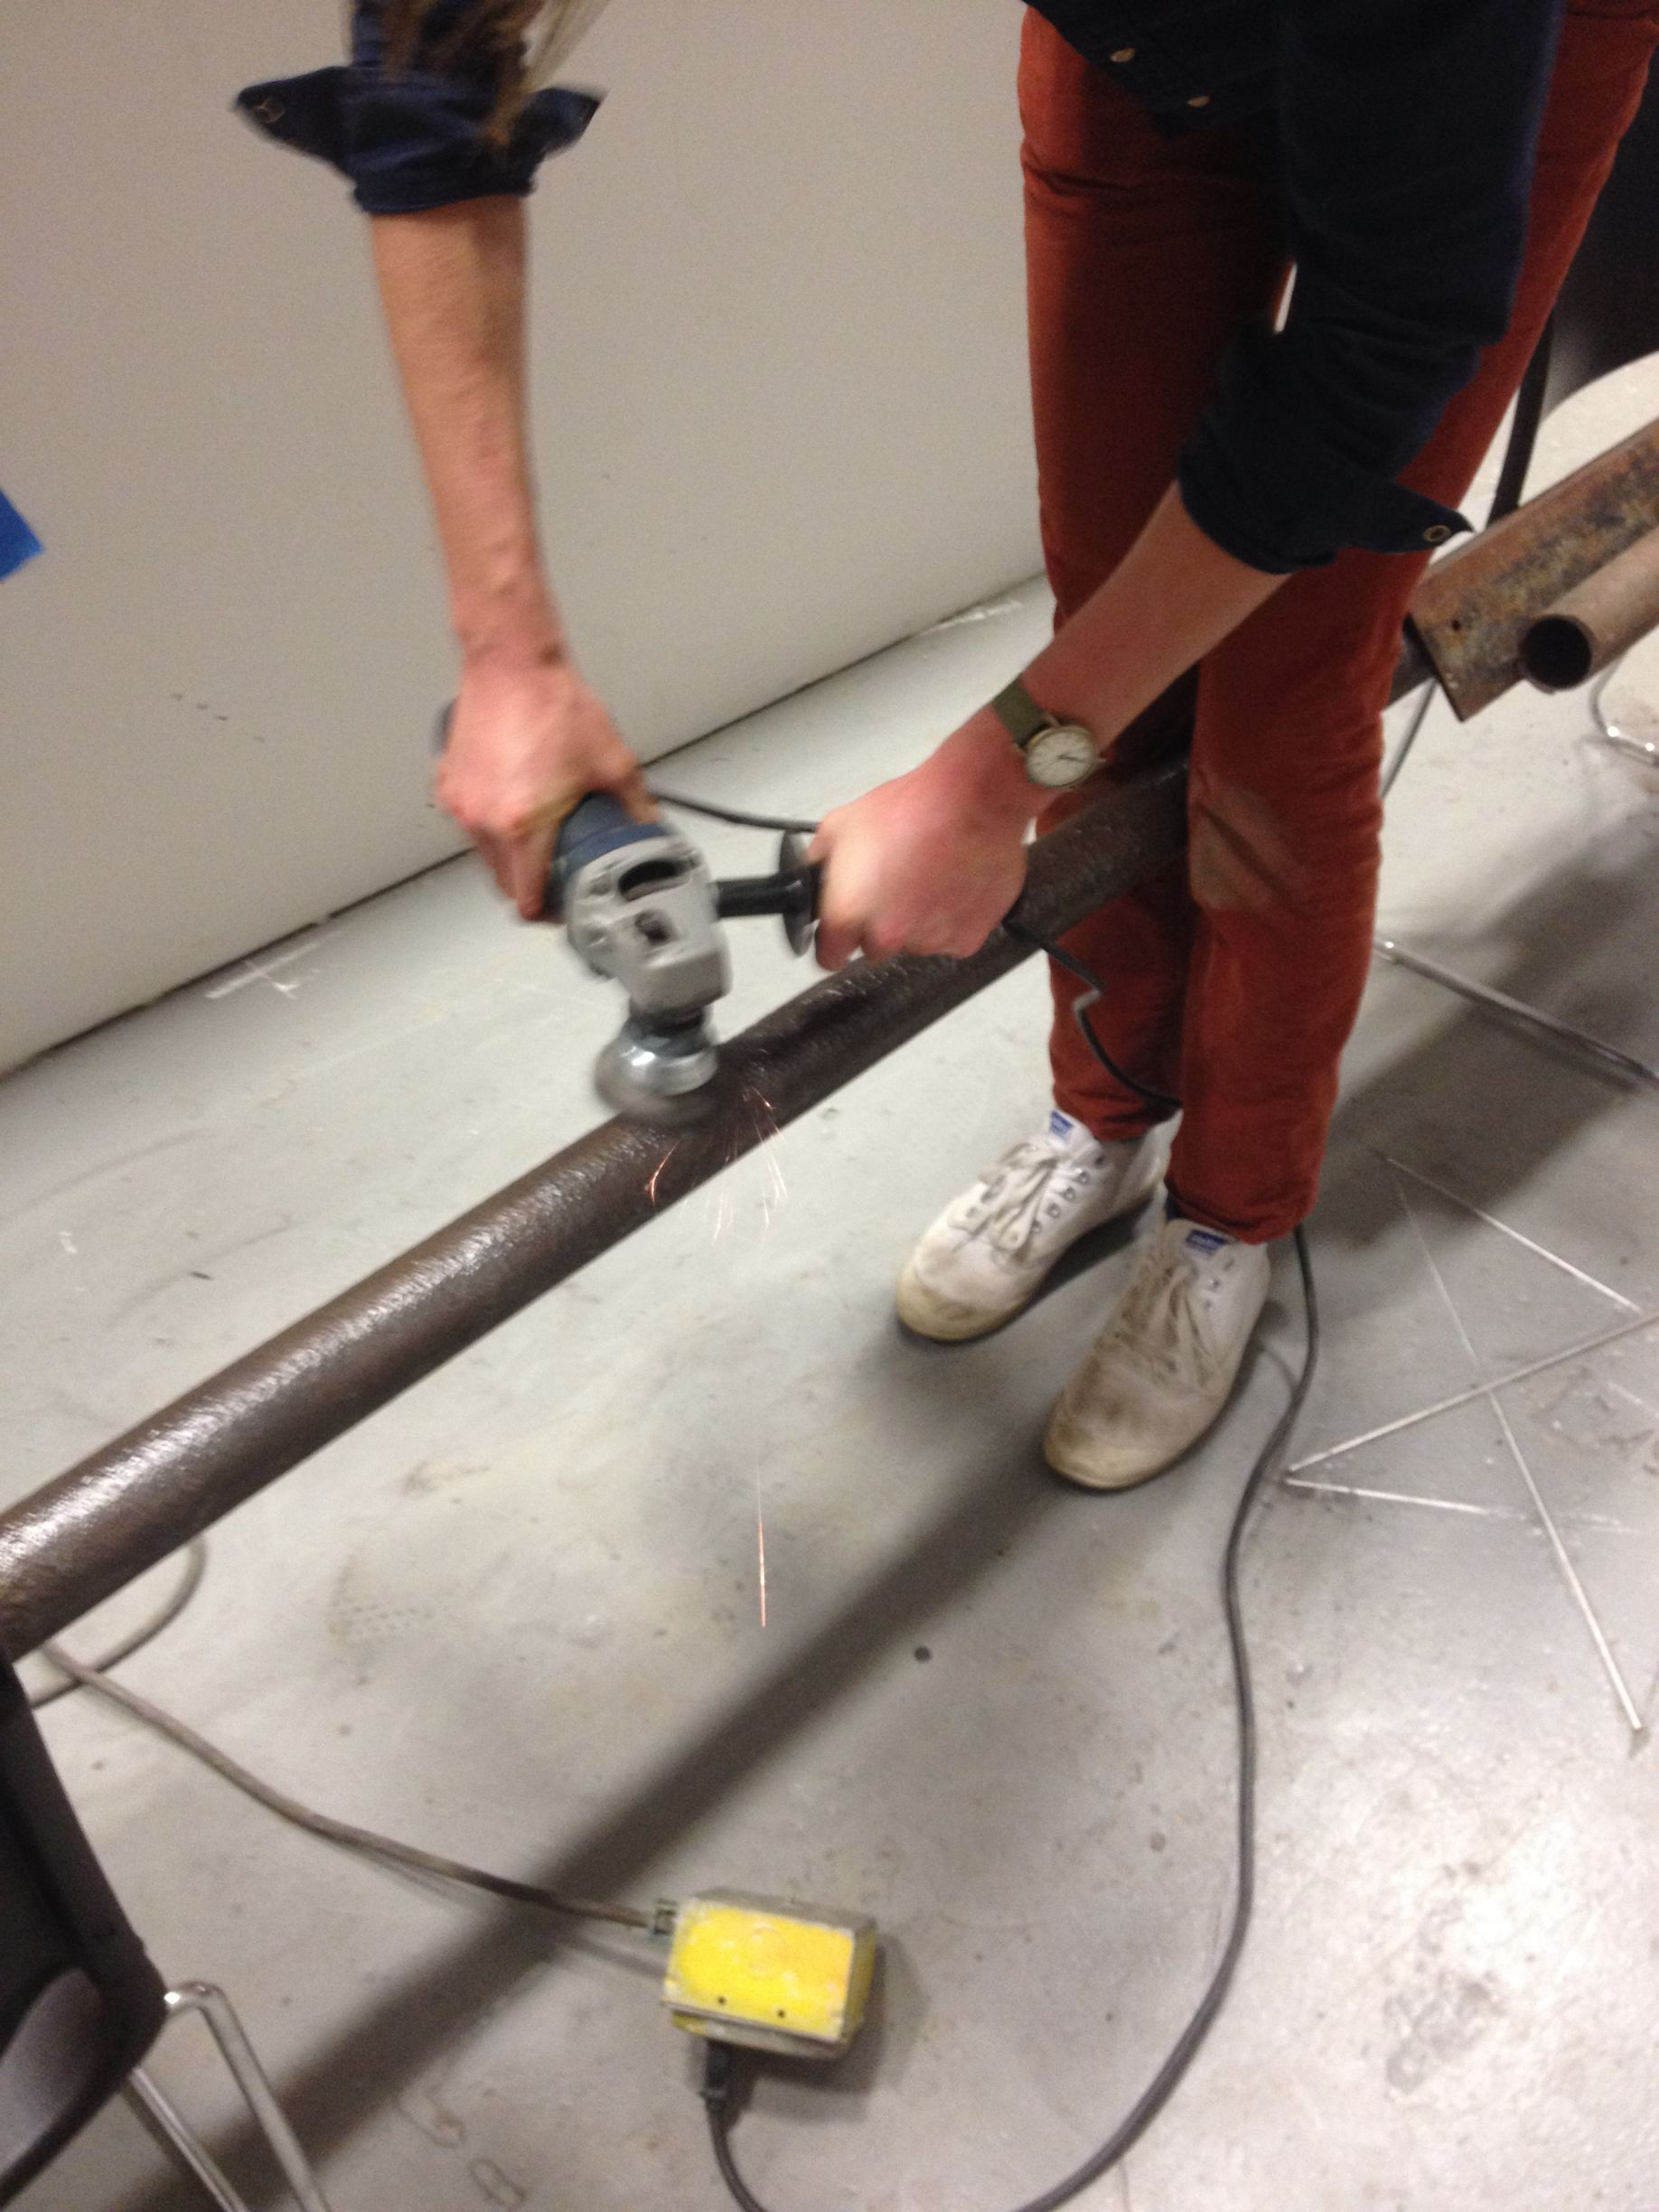
\includegraphics[scale=0.12]{roofmount/03.jpeg}
\end{center}


We then MIG welded the pipe to the plate. We reinforced the weld with a couple extra beads because most of the force in the system will be directed to this point.

\begin{center}
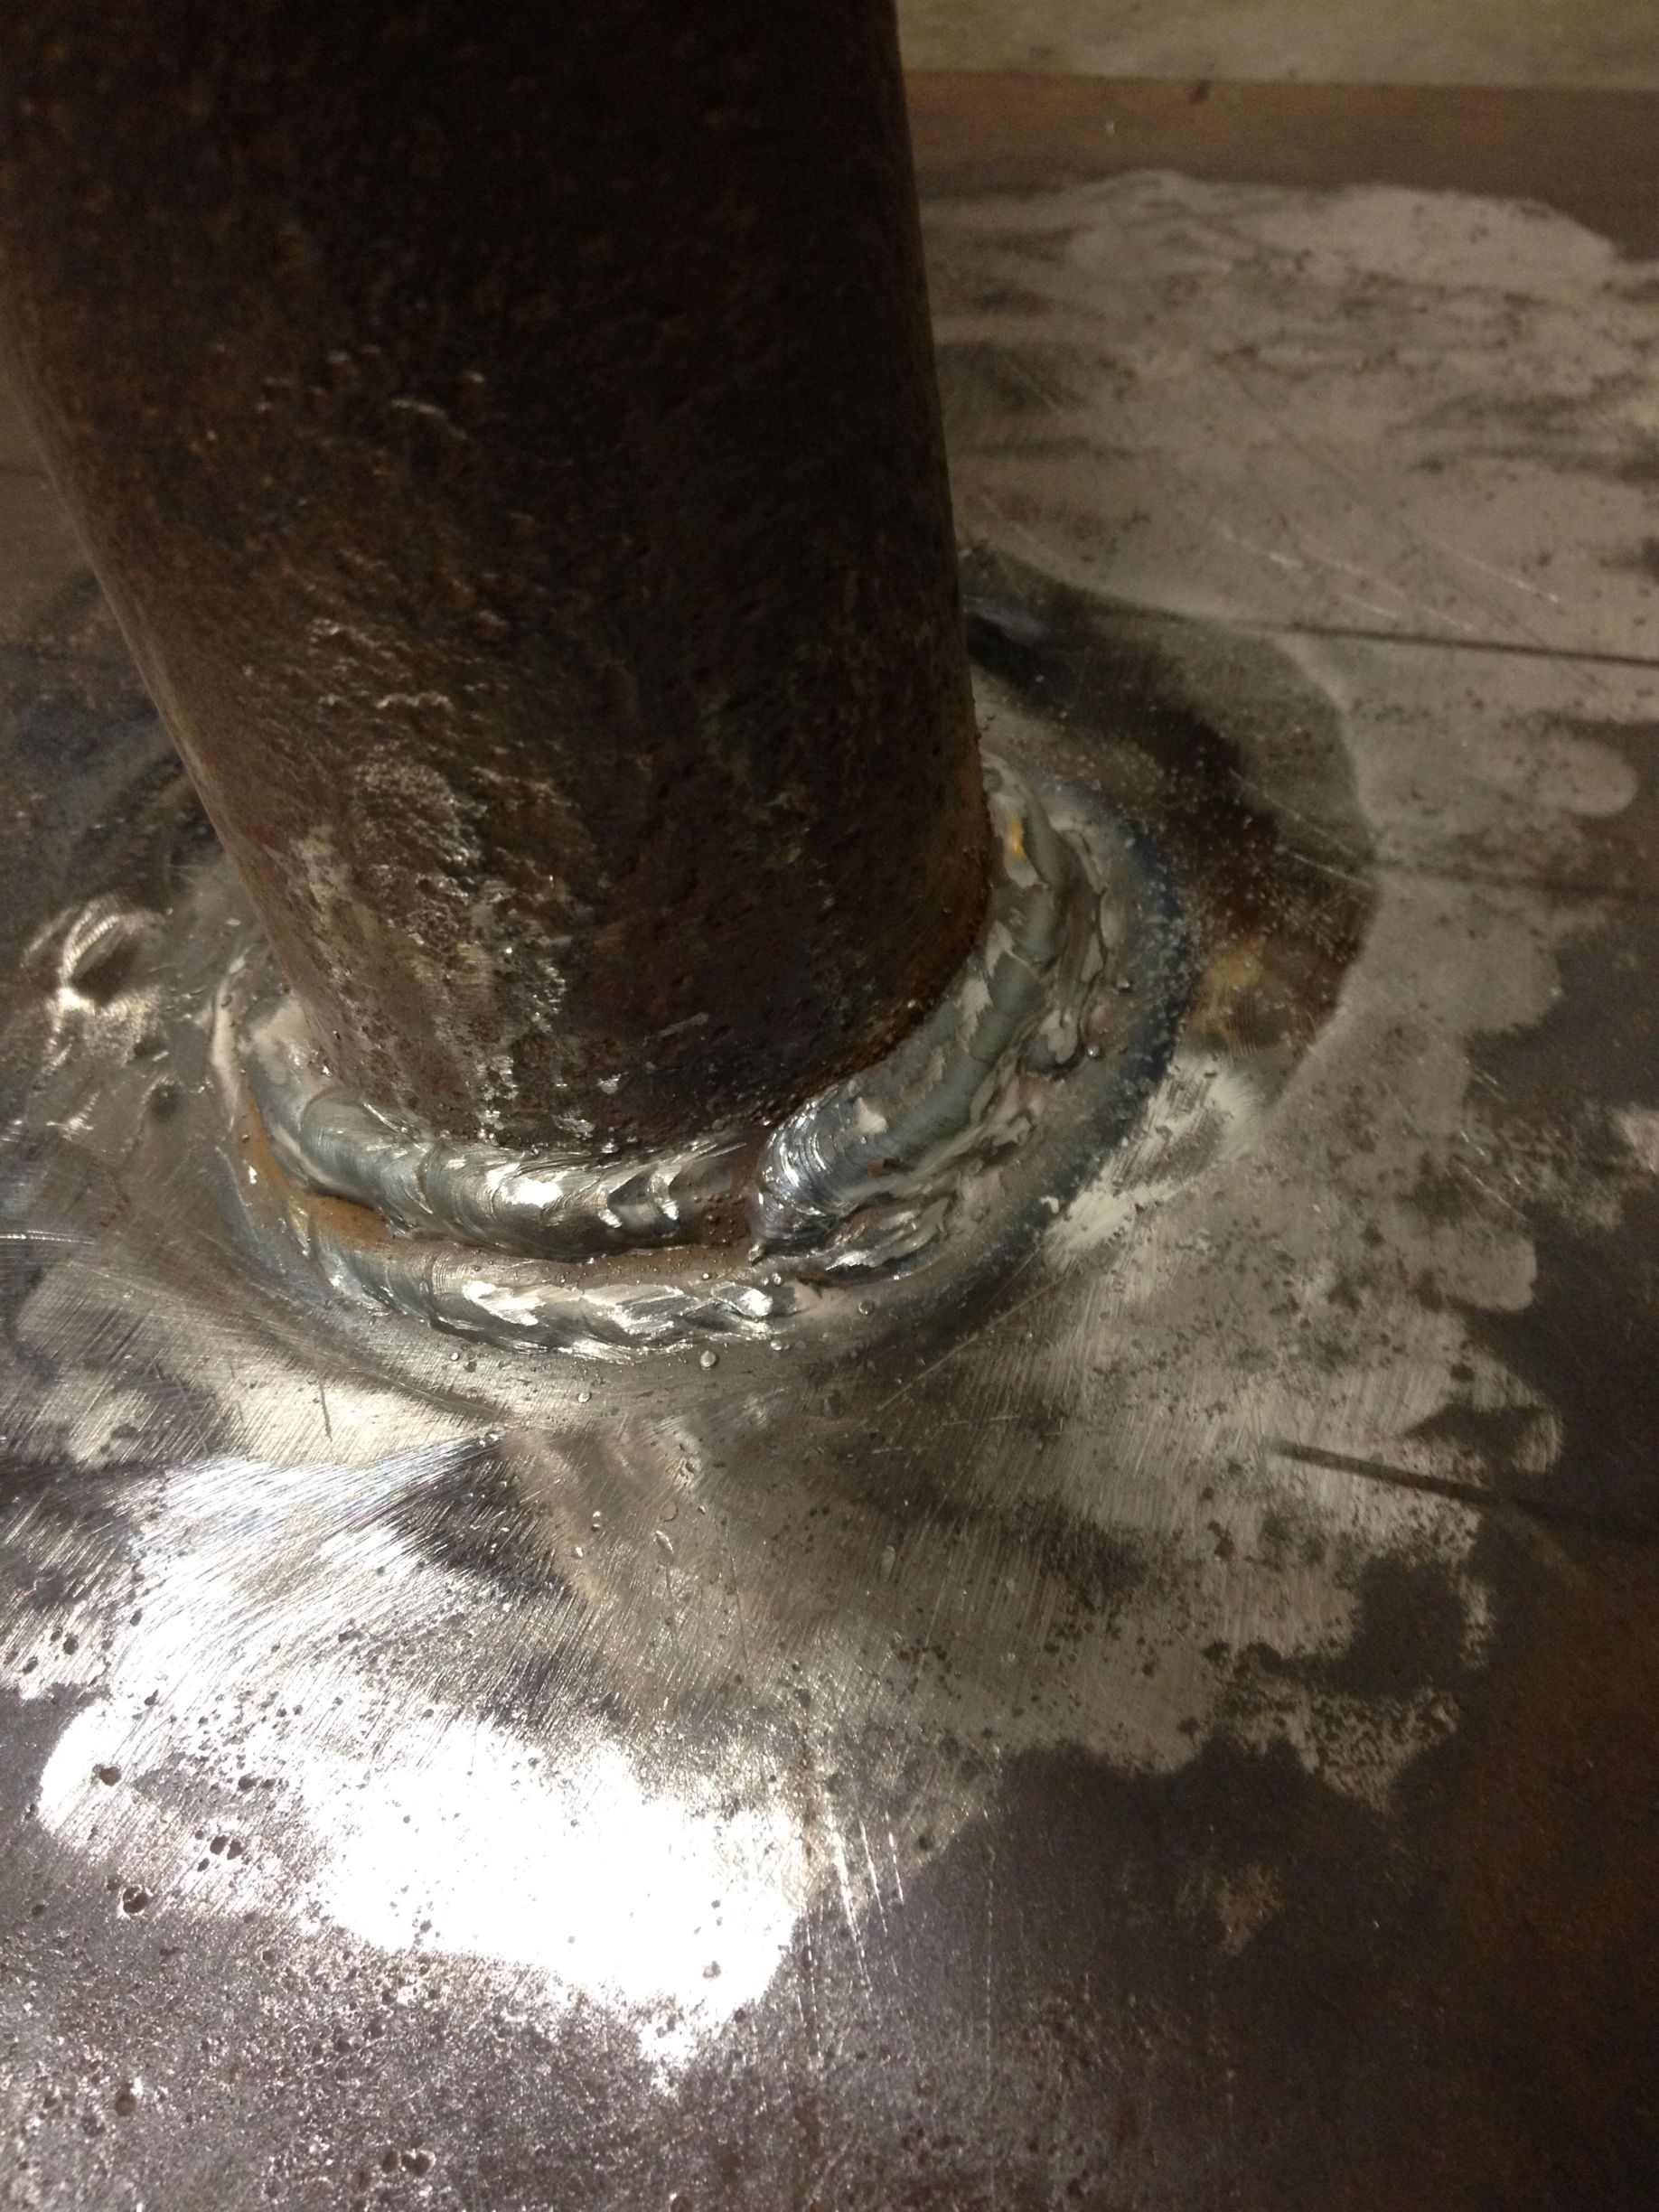
\includegraphics[scale=0.12]{roofmount/04.jpeg}
\end{center}


The real trick was getting the pipe perpendicular to the plate.

\begin{center}
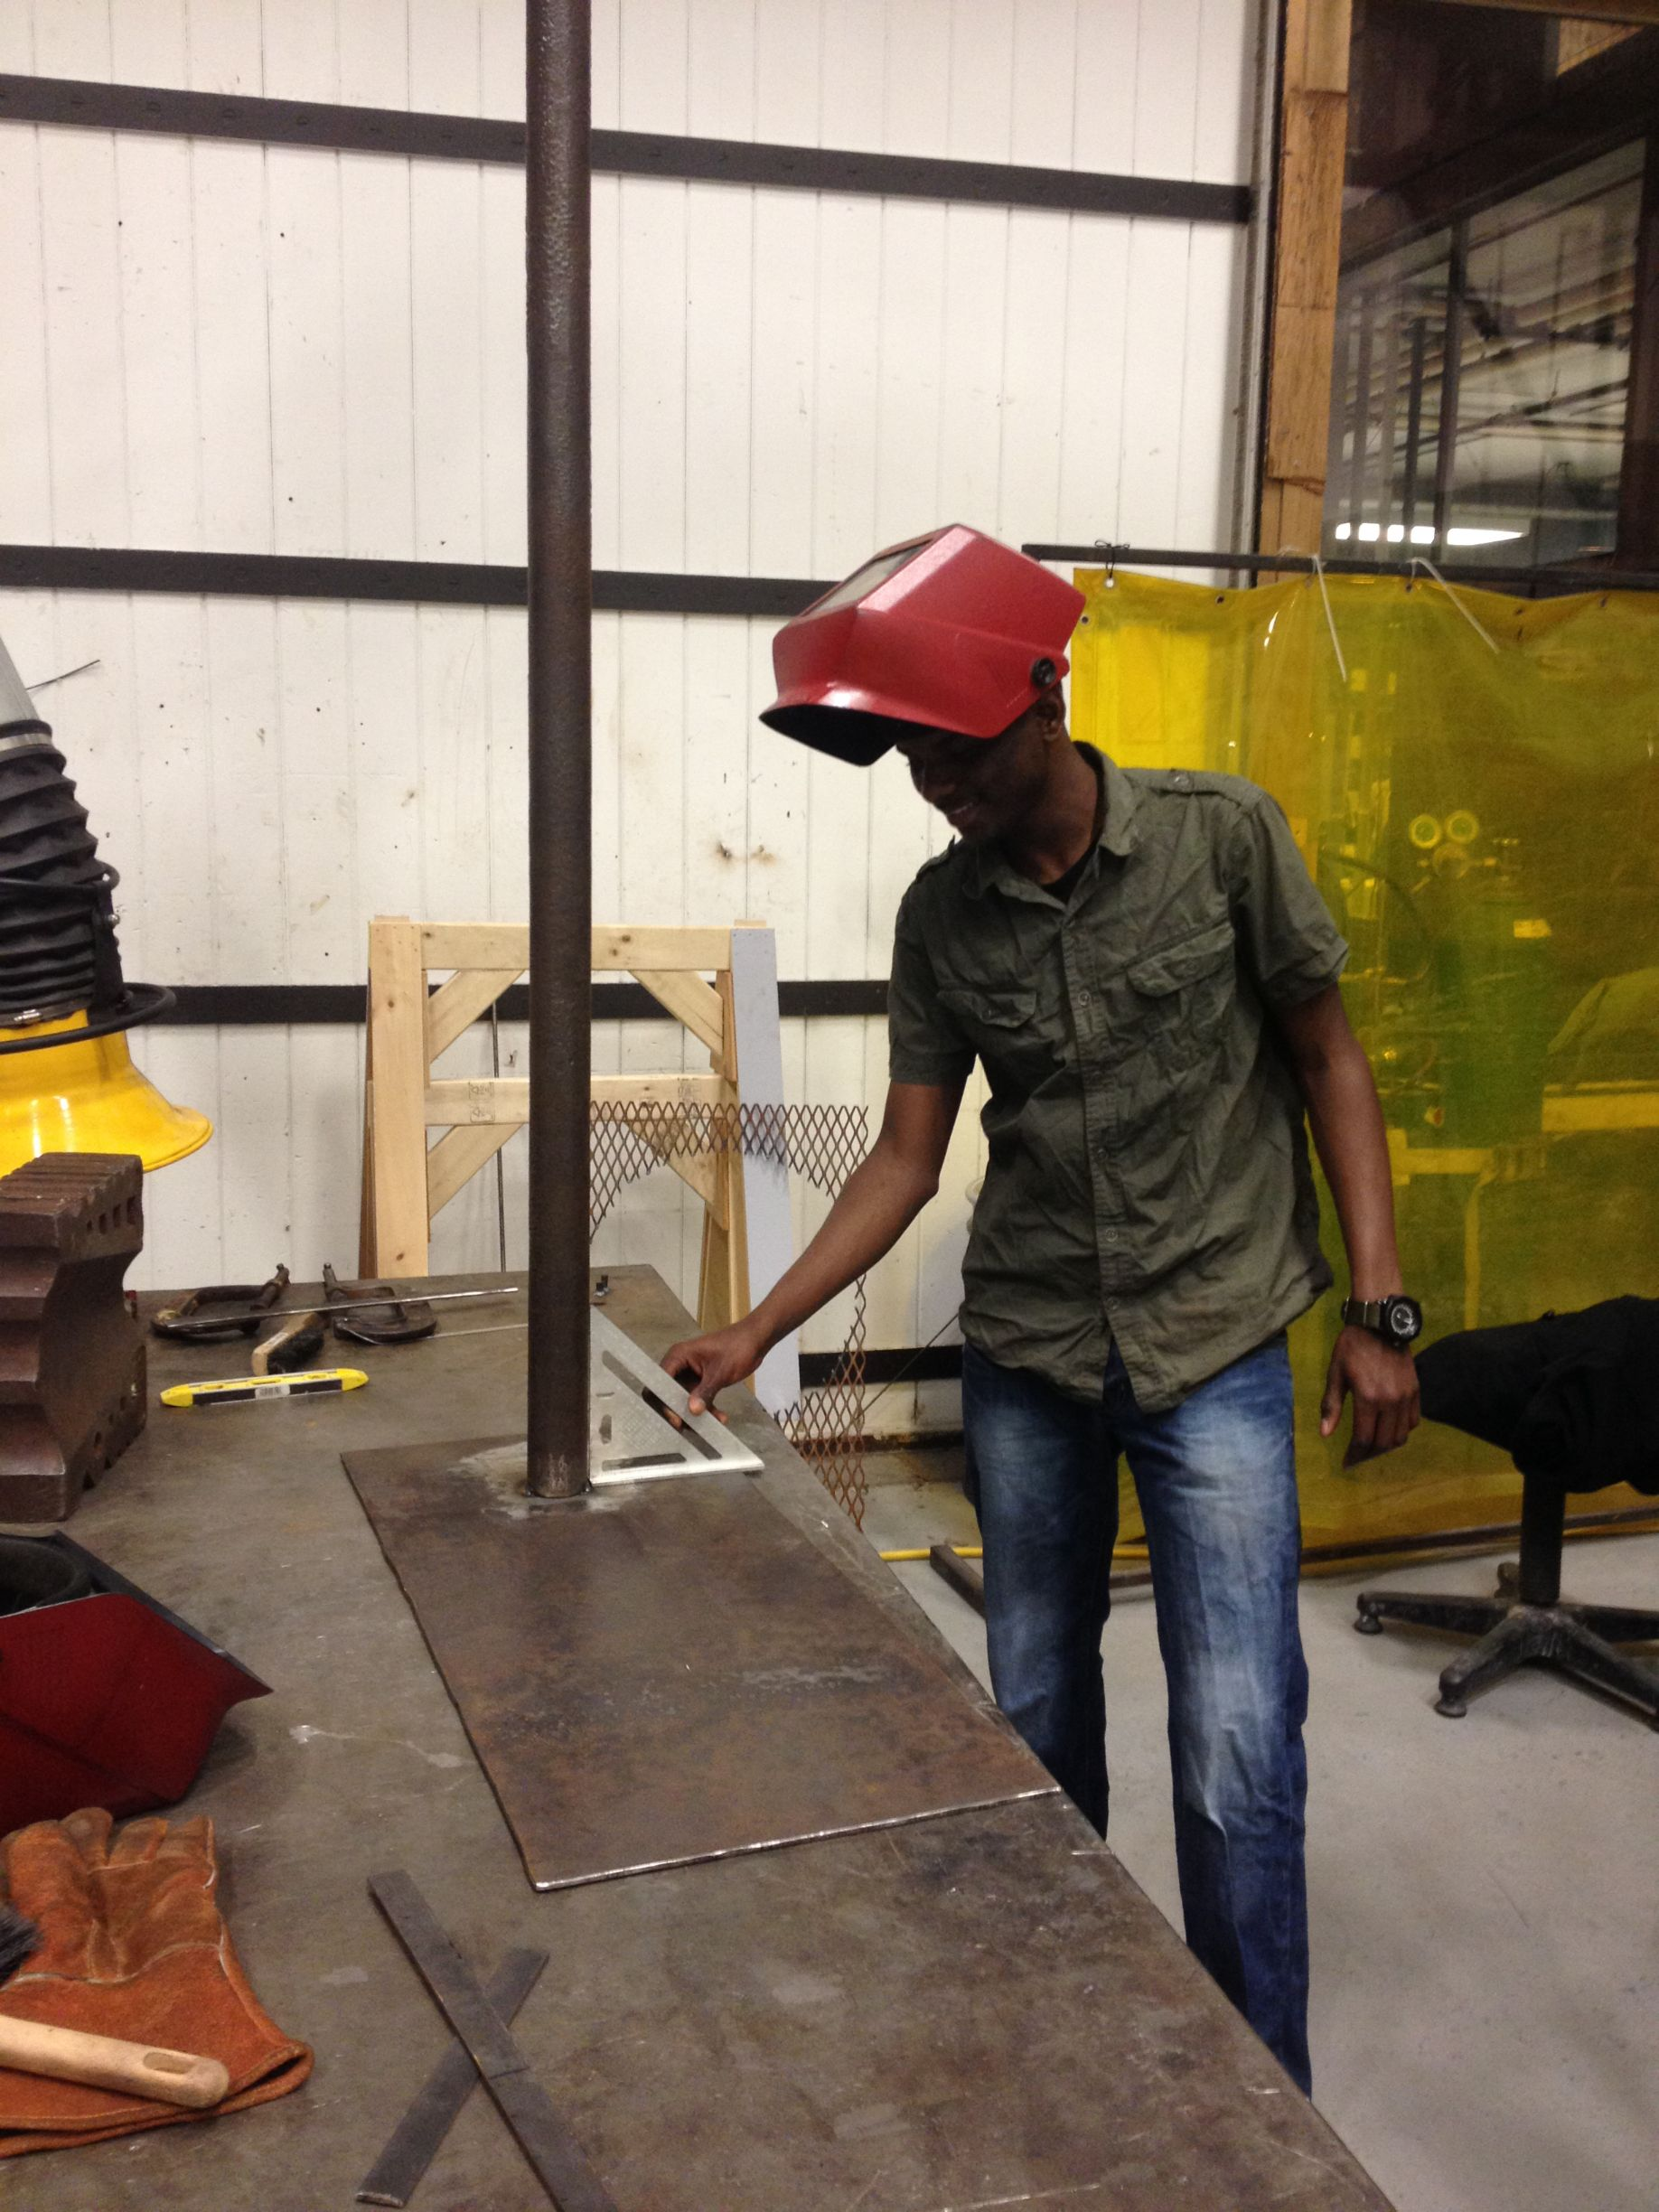
\includegraphics[scale=0.12]{roofmount/05.jpeg}
\end{center}


We ended up clamping the plate on one side of the table and then using the corner of the table as a perpendicular straight edge in two dimensions.

After some tests we realized the weight of the pipe was warping the plate so we successfully reinforced it with some angle iron.

\begin{center}
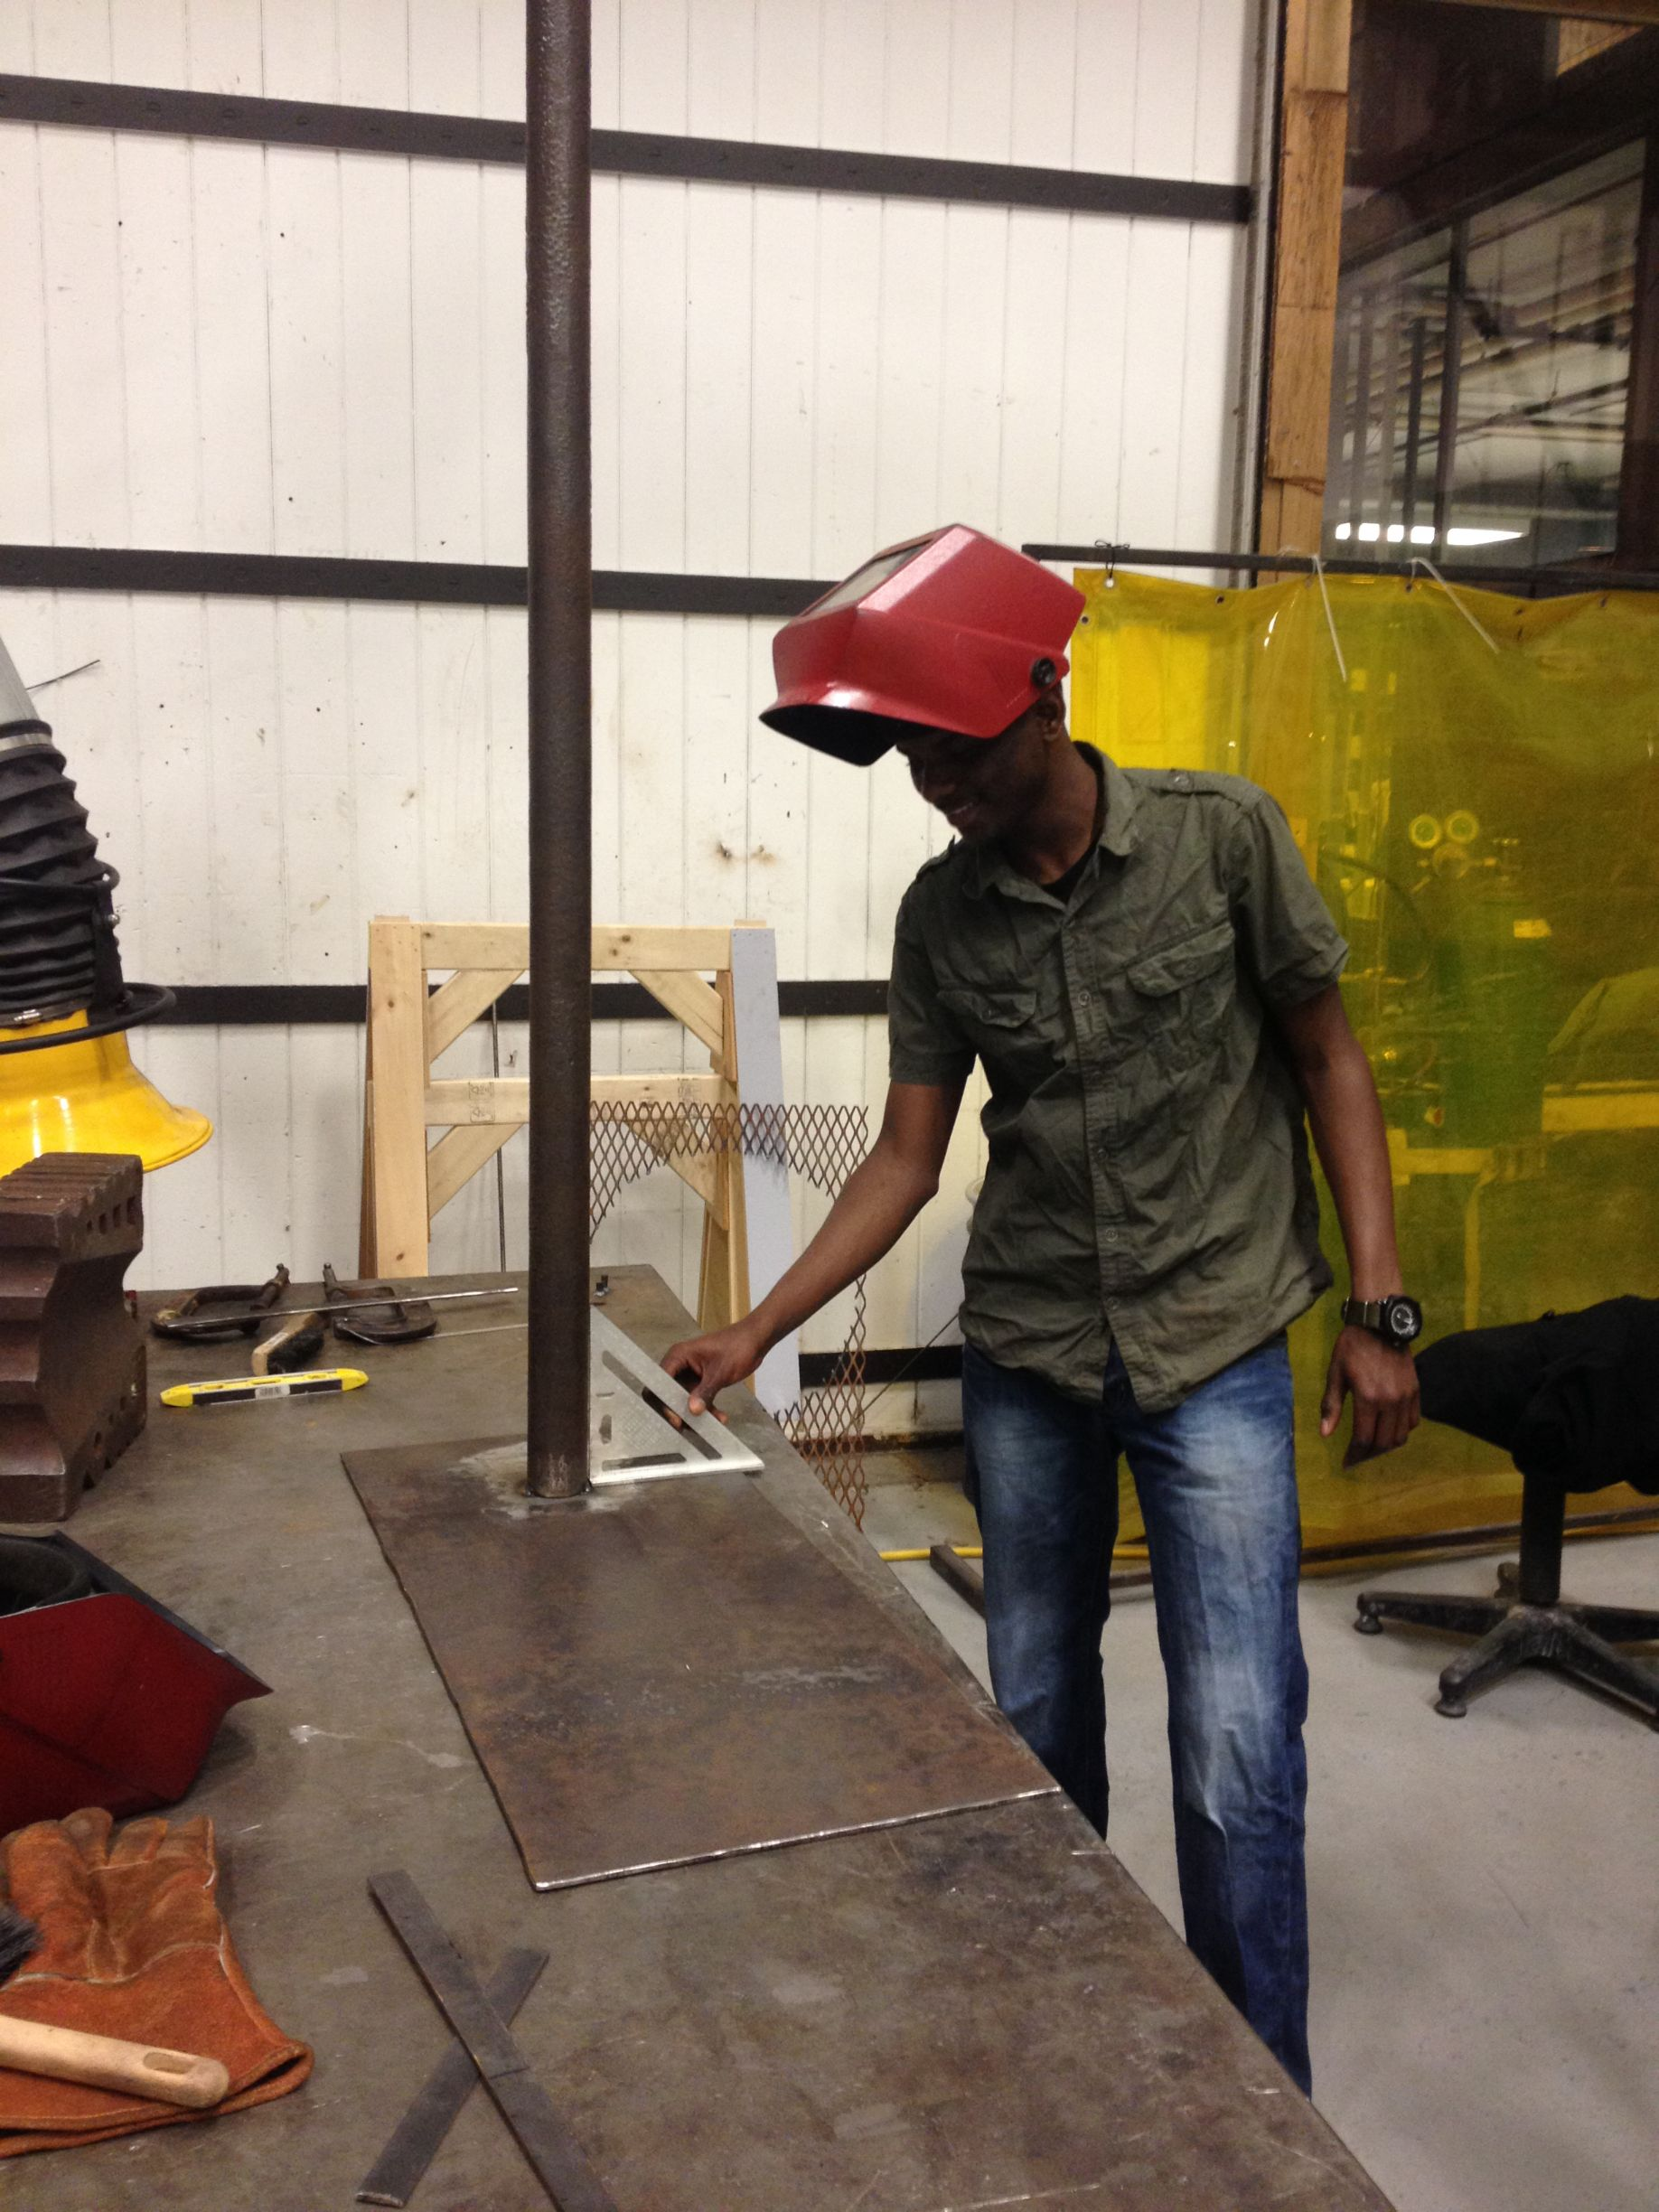
\includegraphics[scale=0.12]{roofmount/05.jpeg}
\end{center}

%%%%%%%%%%%%%%%%%%%%%%%%%%%%%%%%%%%%%%%%

\subsection{Dish}

We bolted together the central plates, trying to make sure they are parallel to each other.

Then we bolted on half of the dish arms which confirmed the accuracy of our central plate construction. This is as much of the dish as will fit out the door to the roof we will be mounting the dish on. The rest of the assembly happened on site.



\begin{center}
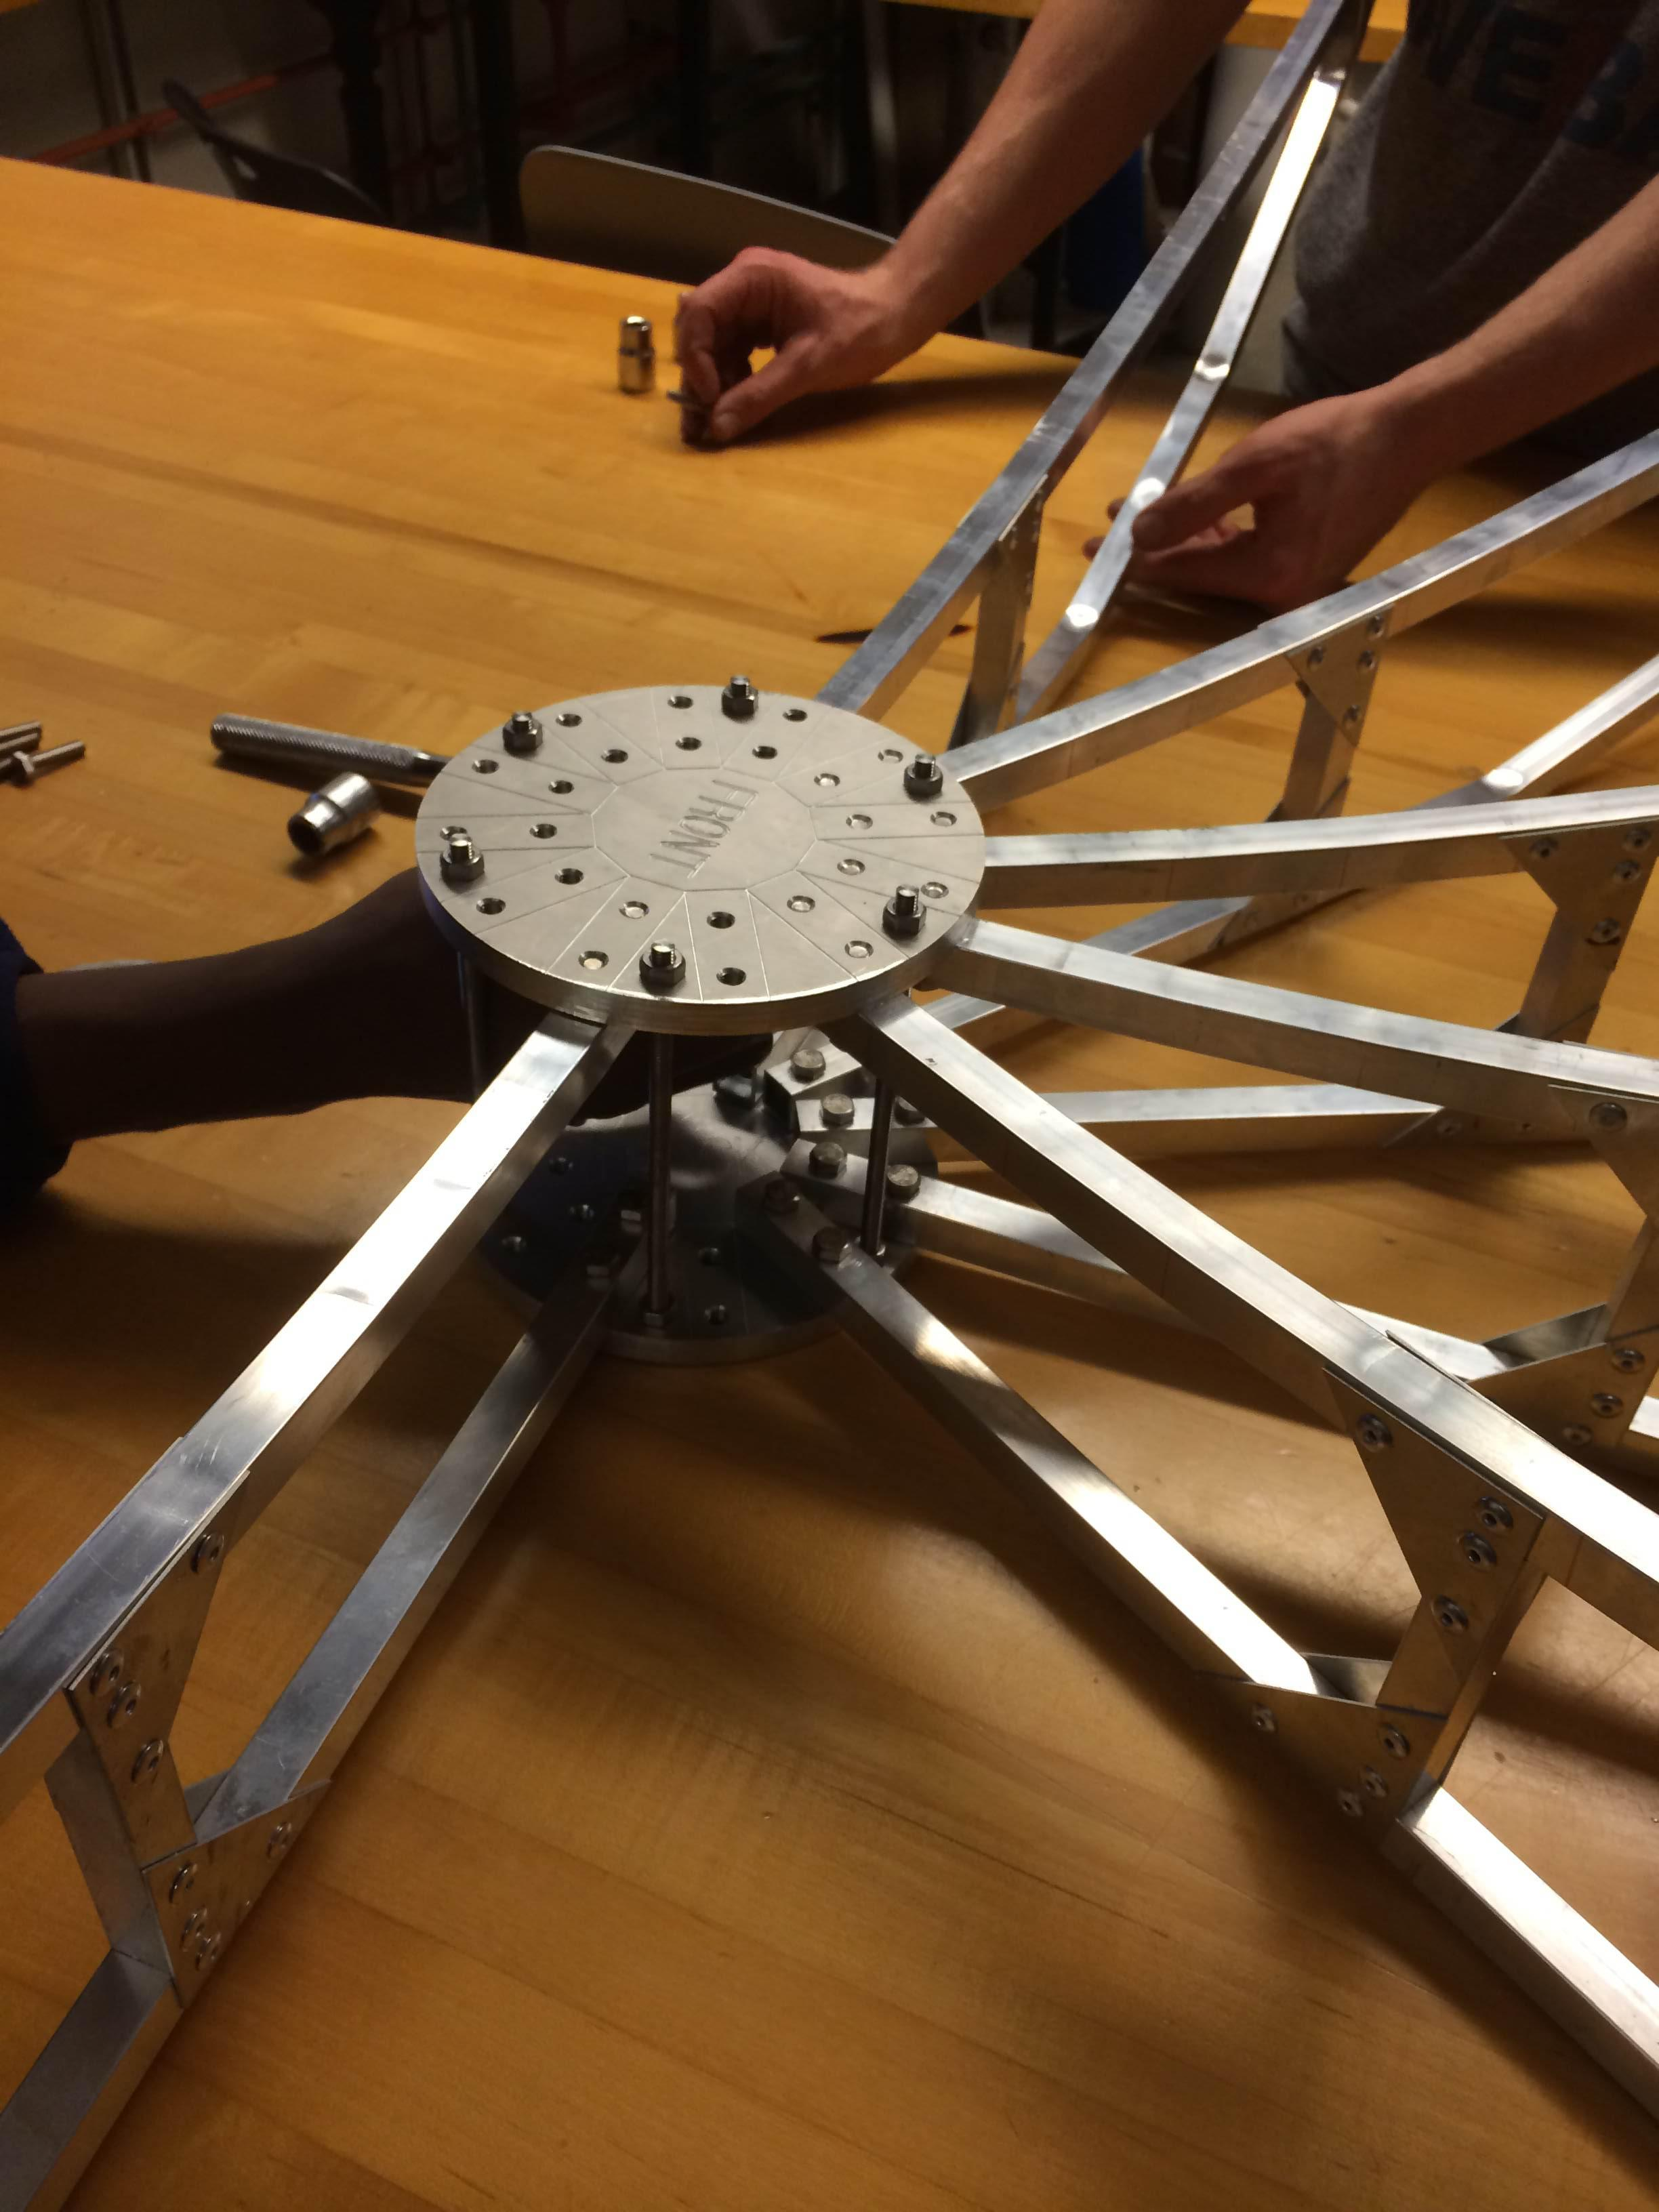
\includegraphics[scale=0.12]{dish/01.jpeg}
\end{center}

\begin{center}
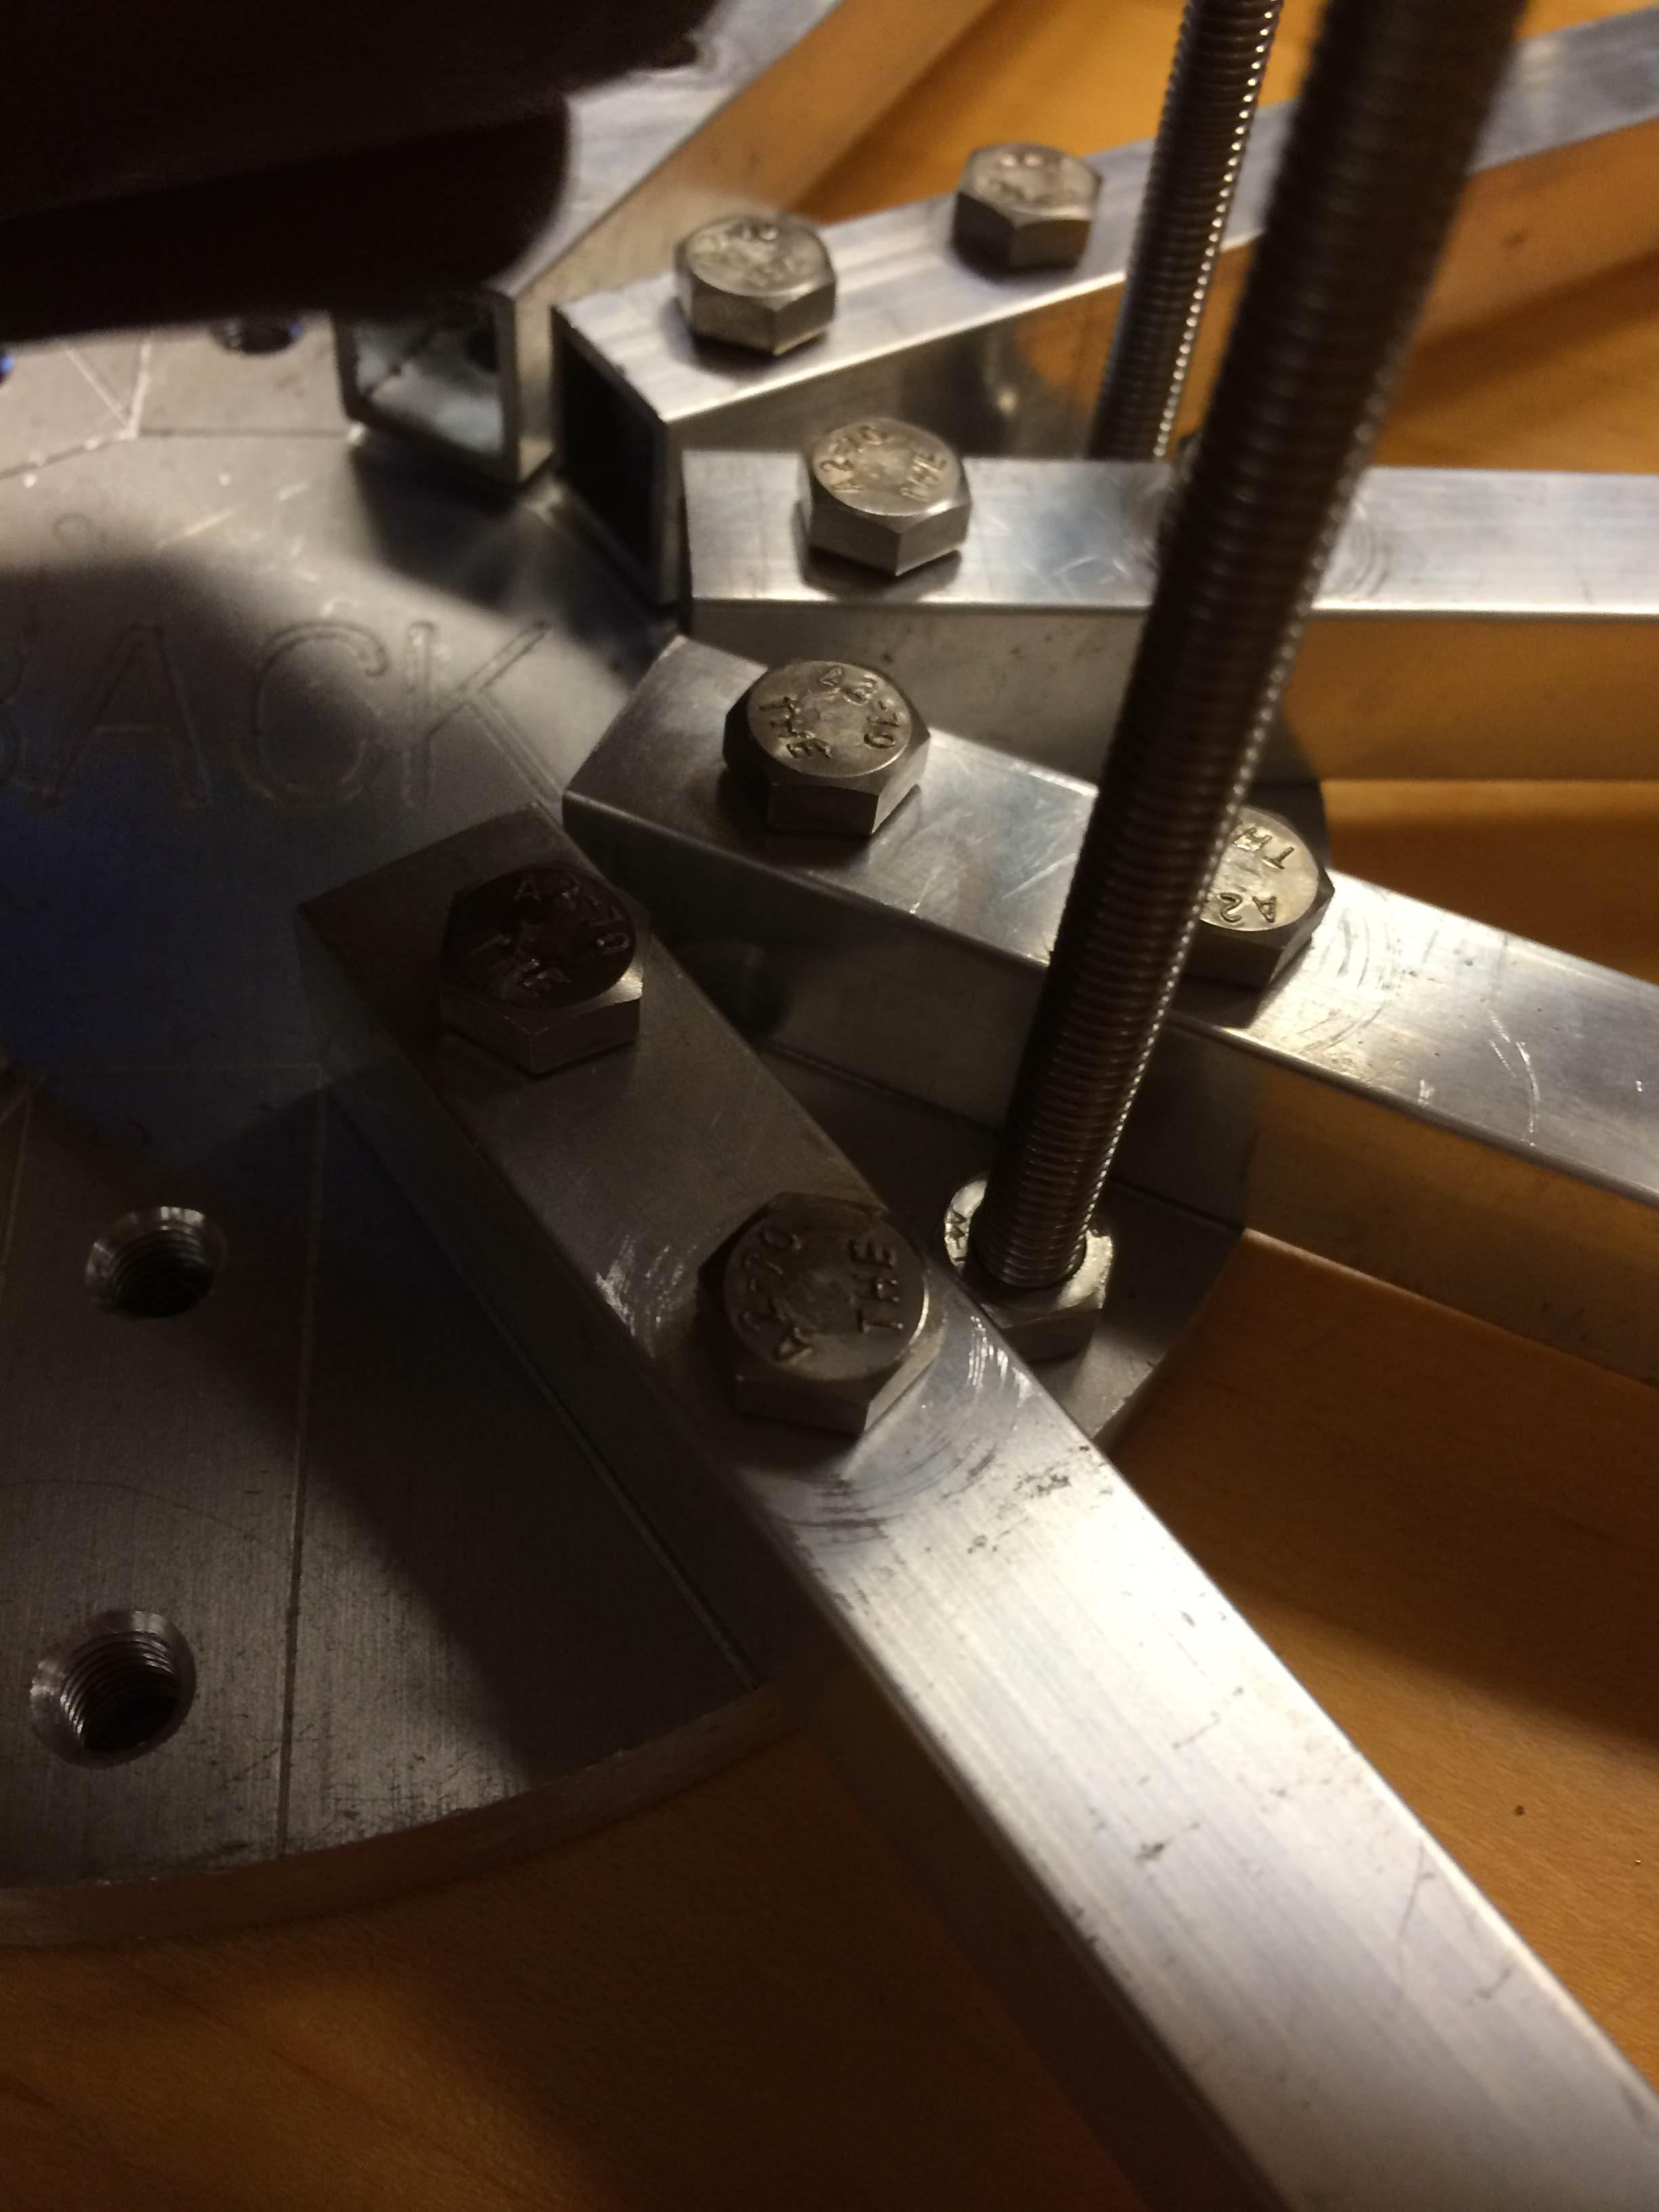
\includegraphics[scale=0.12]{dish/02.jpeg}
\end{center}

\begin{center}
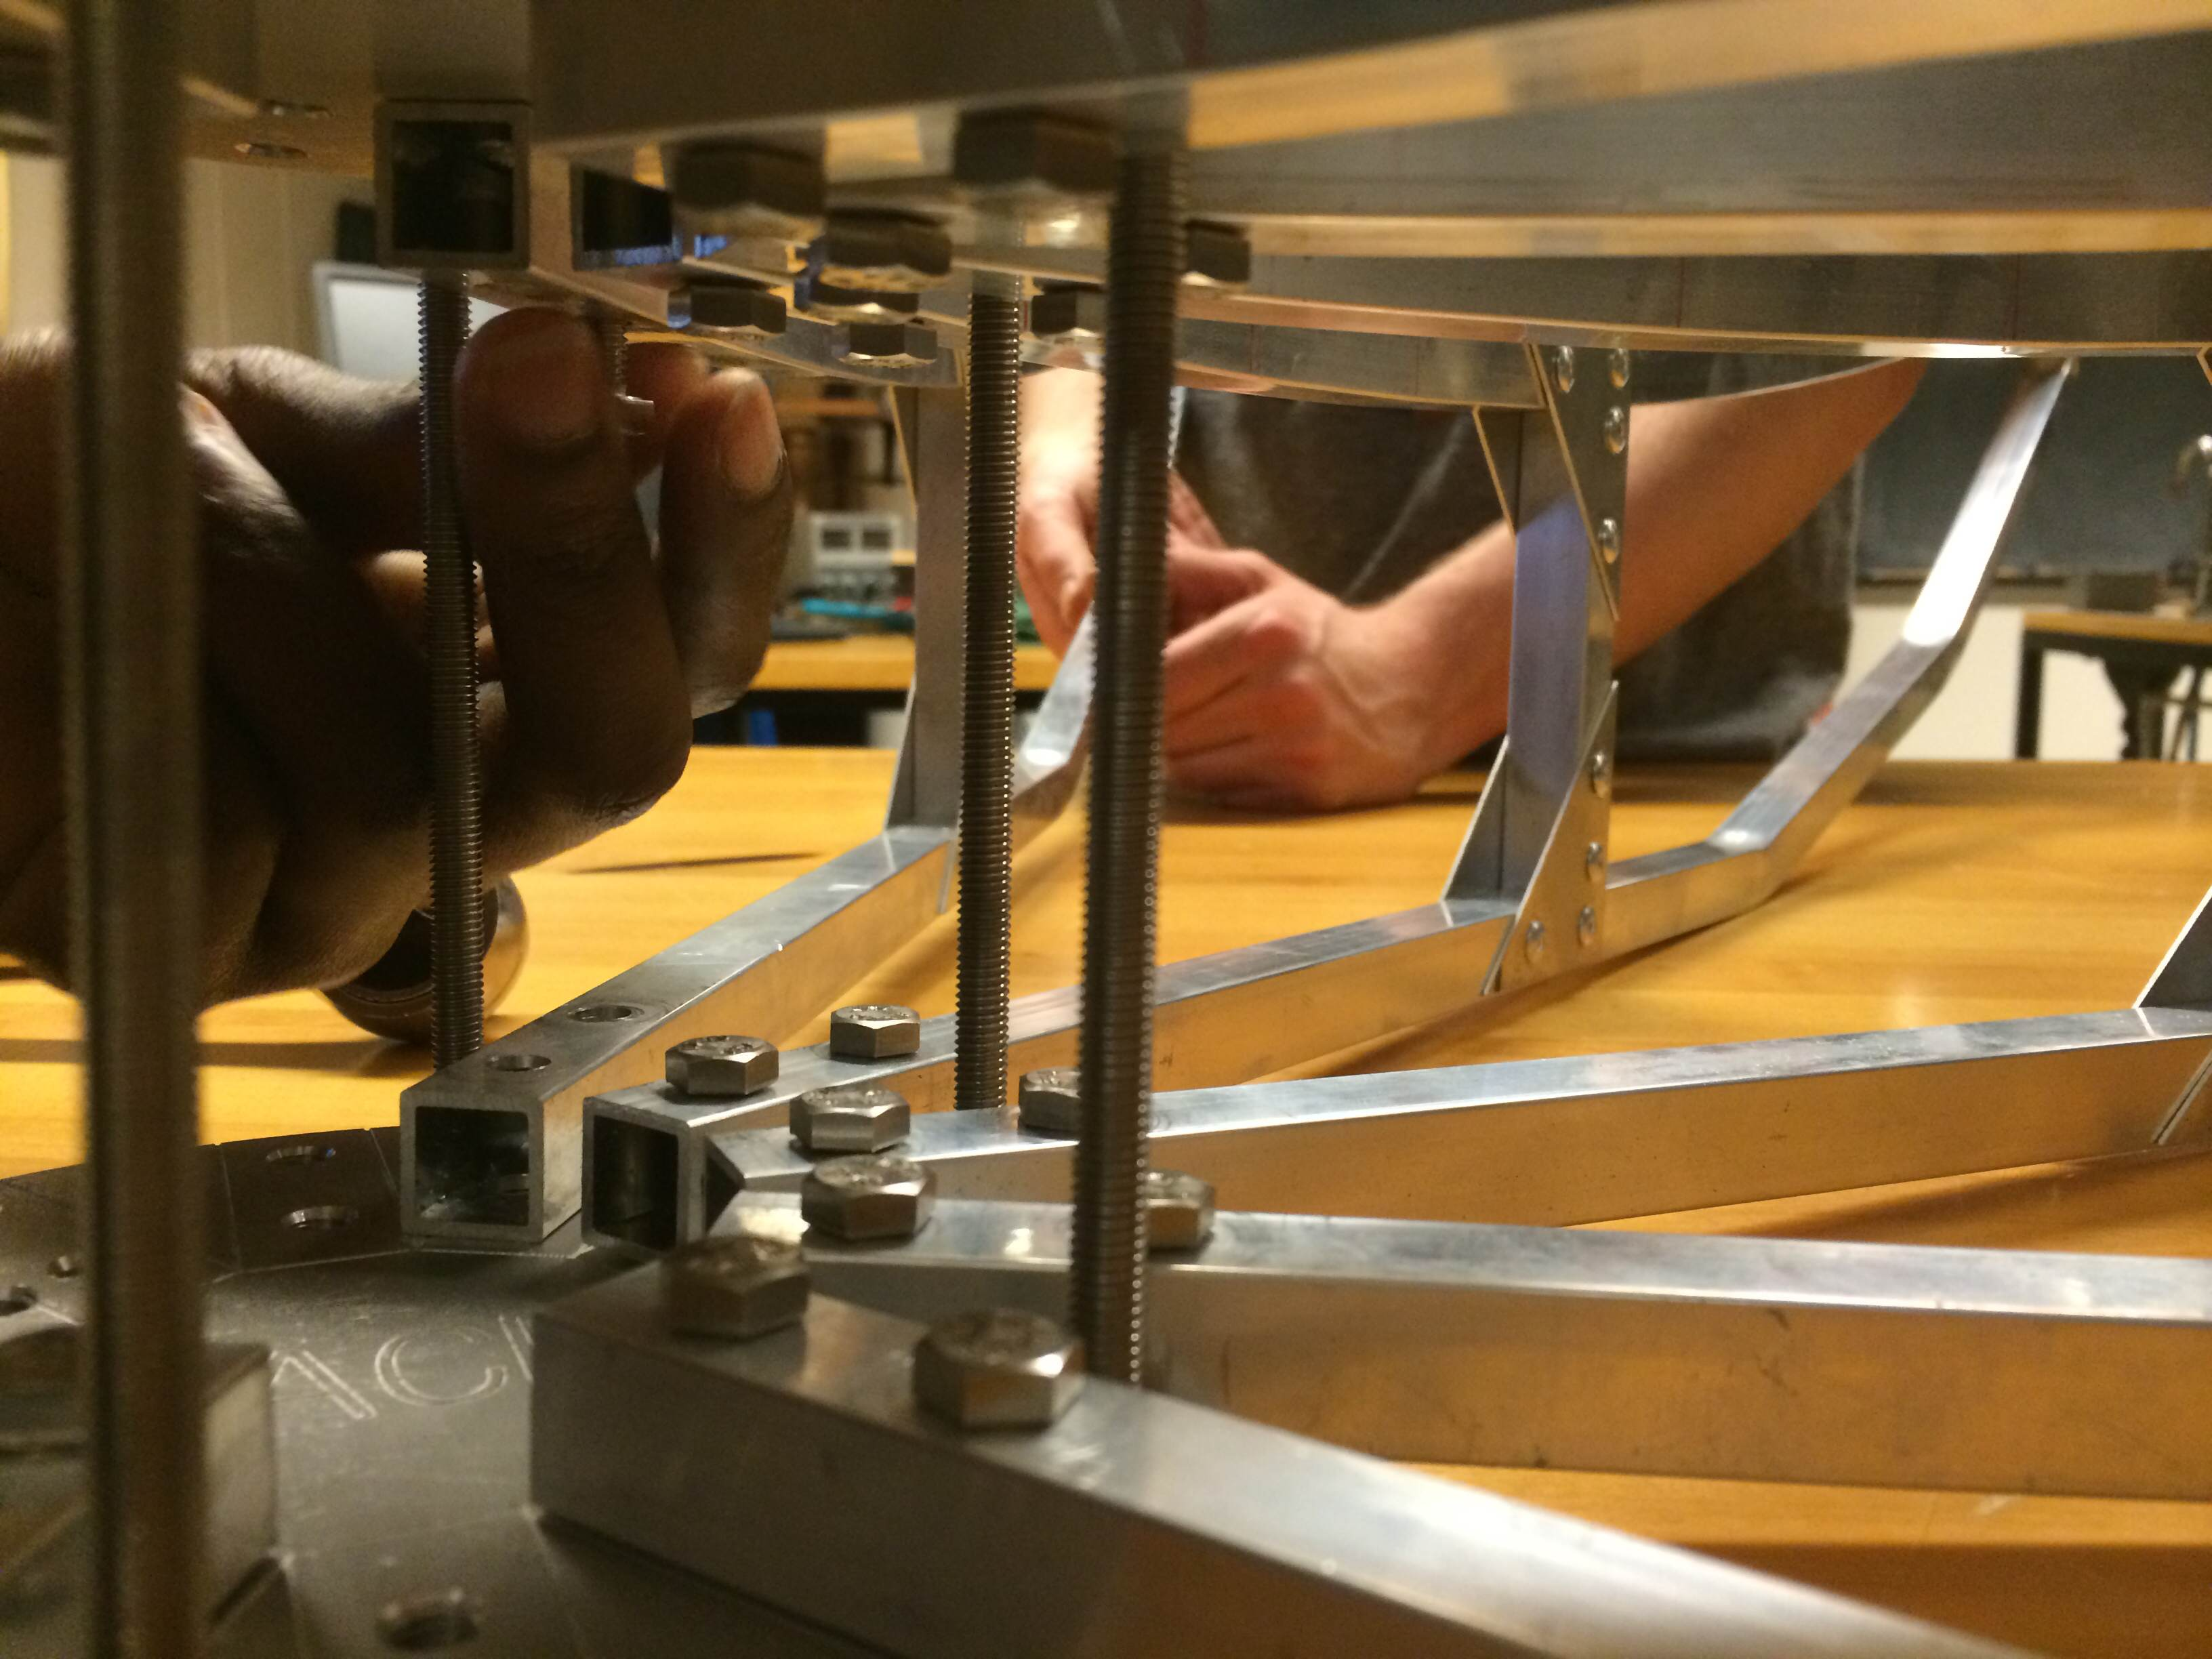
\includegraphics[scale=0.12]{dish/03.jpeg}
\end{center}

Once the ribs are put together and the support rings are in place, we are ready to put on the outer band.

\begin{center}
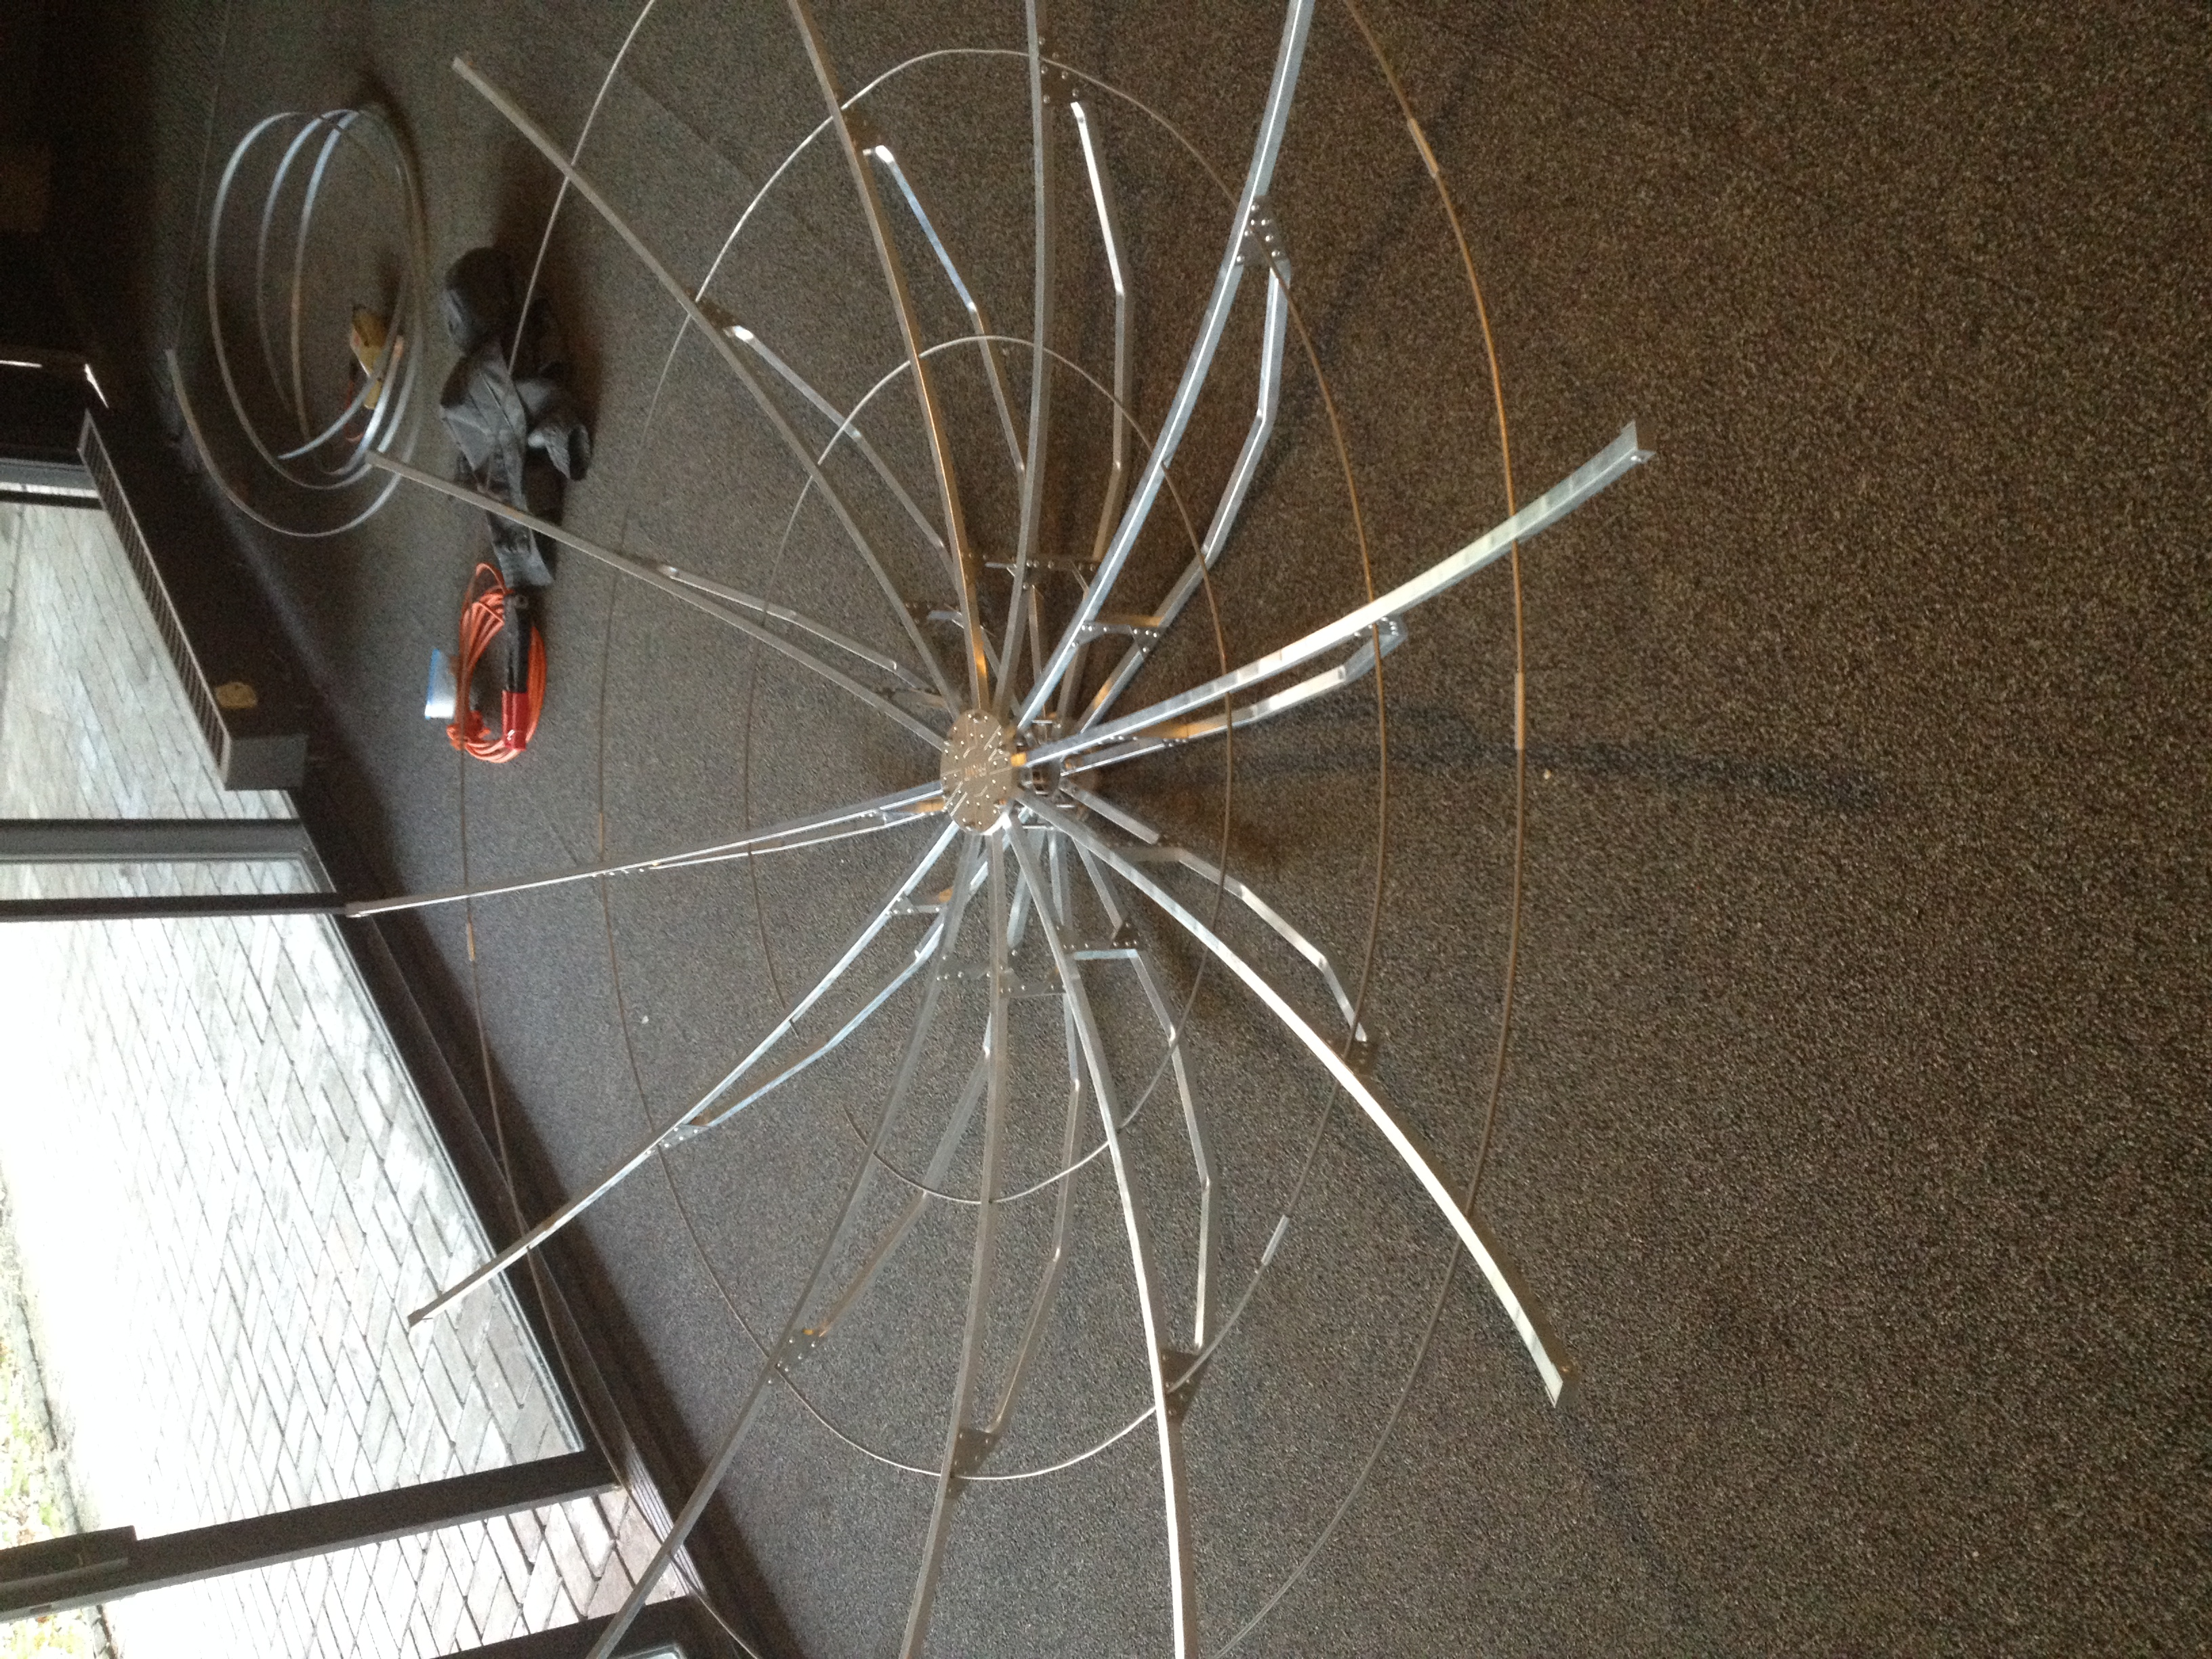
\includegraphics[scale=0.12]{dish/04.jpeg}
\end{center}

To do this, a hammer and tap were used to make dents in the end of the rib and the band

\begin{center}
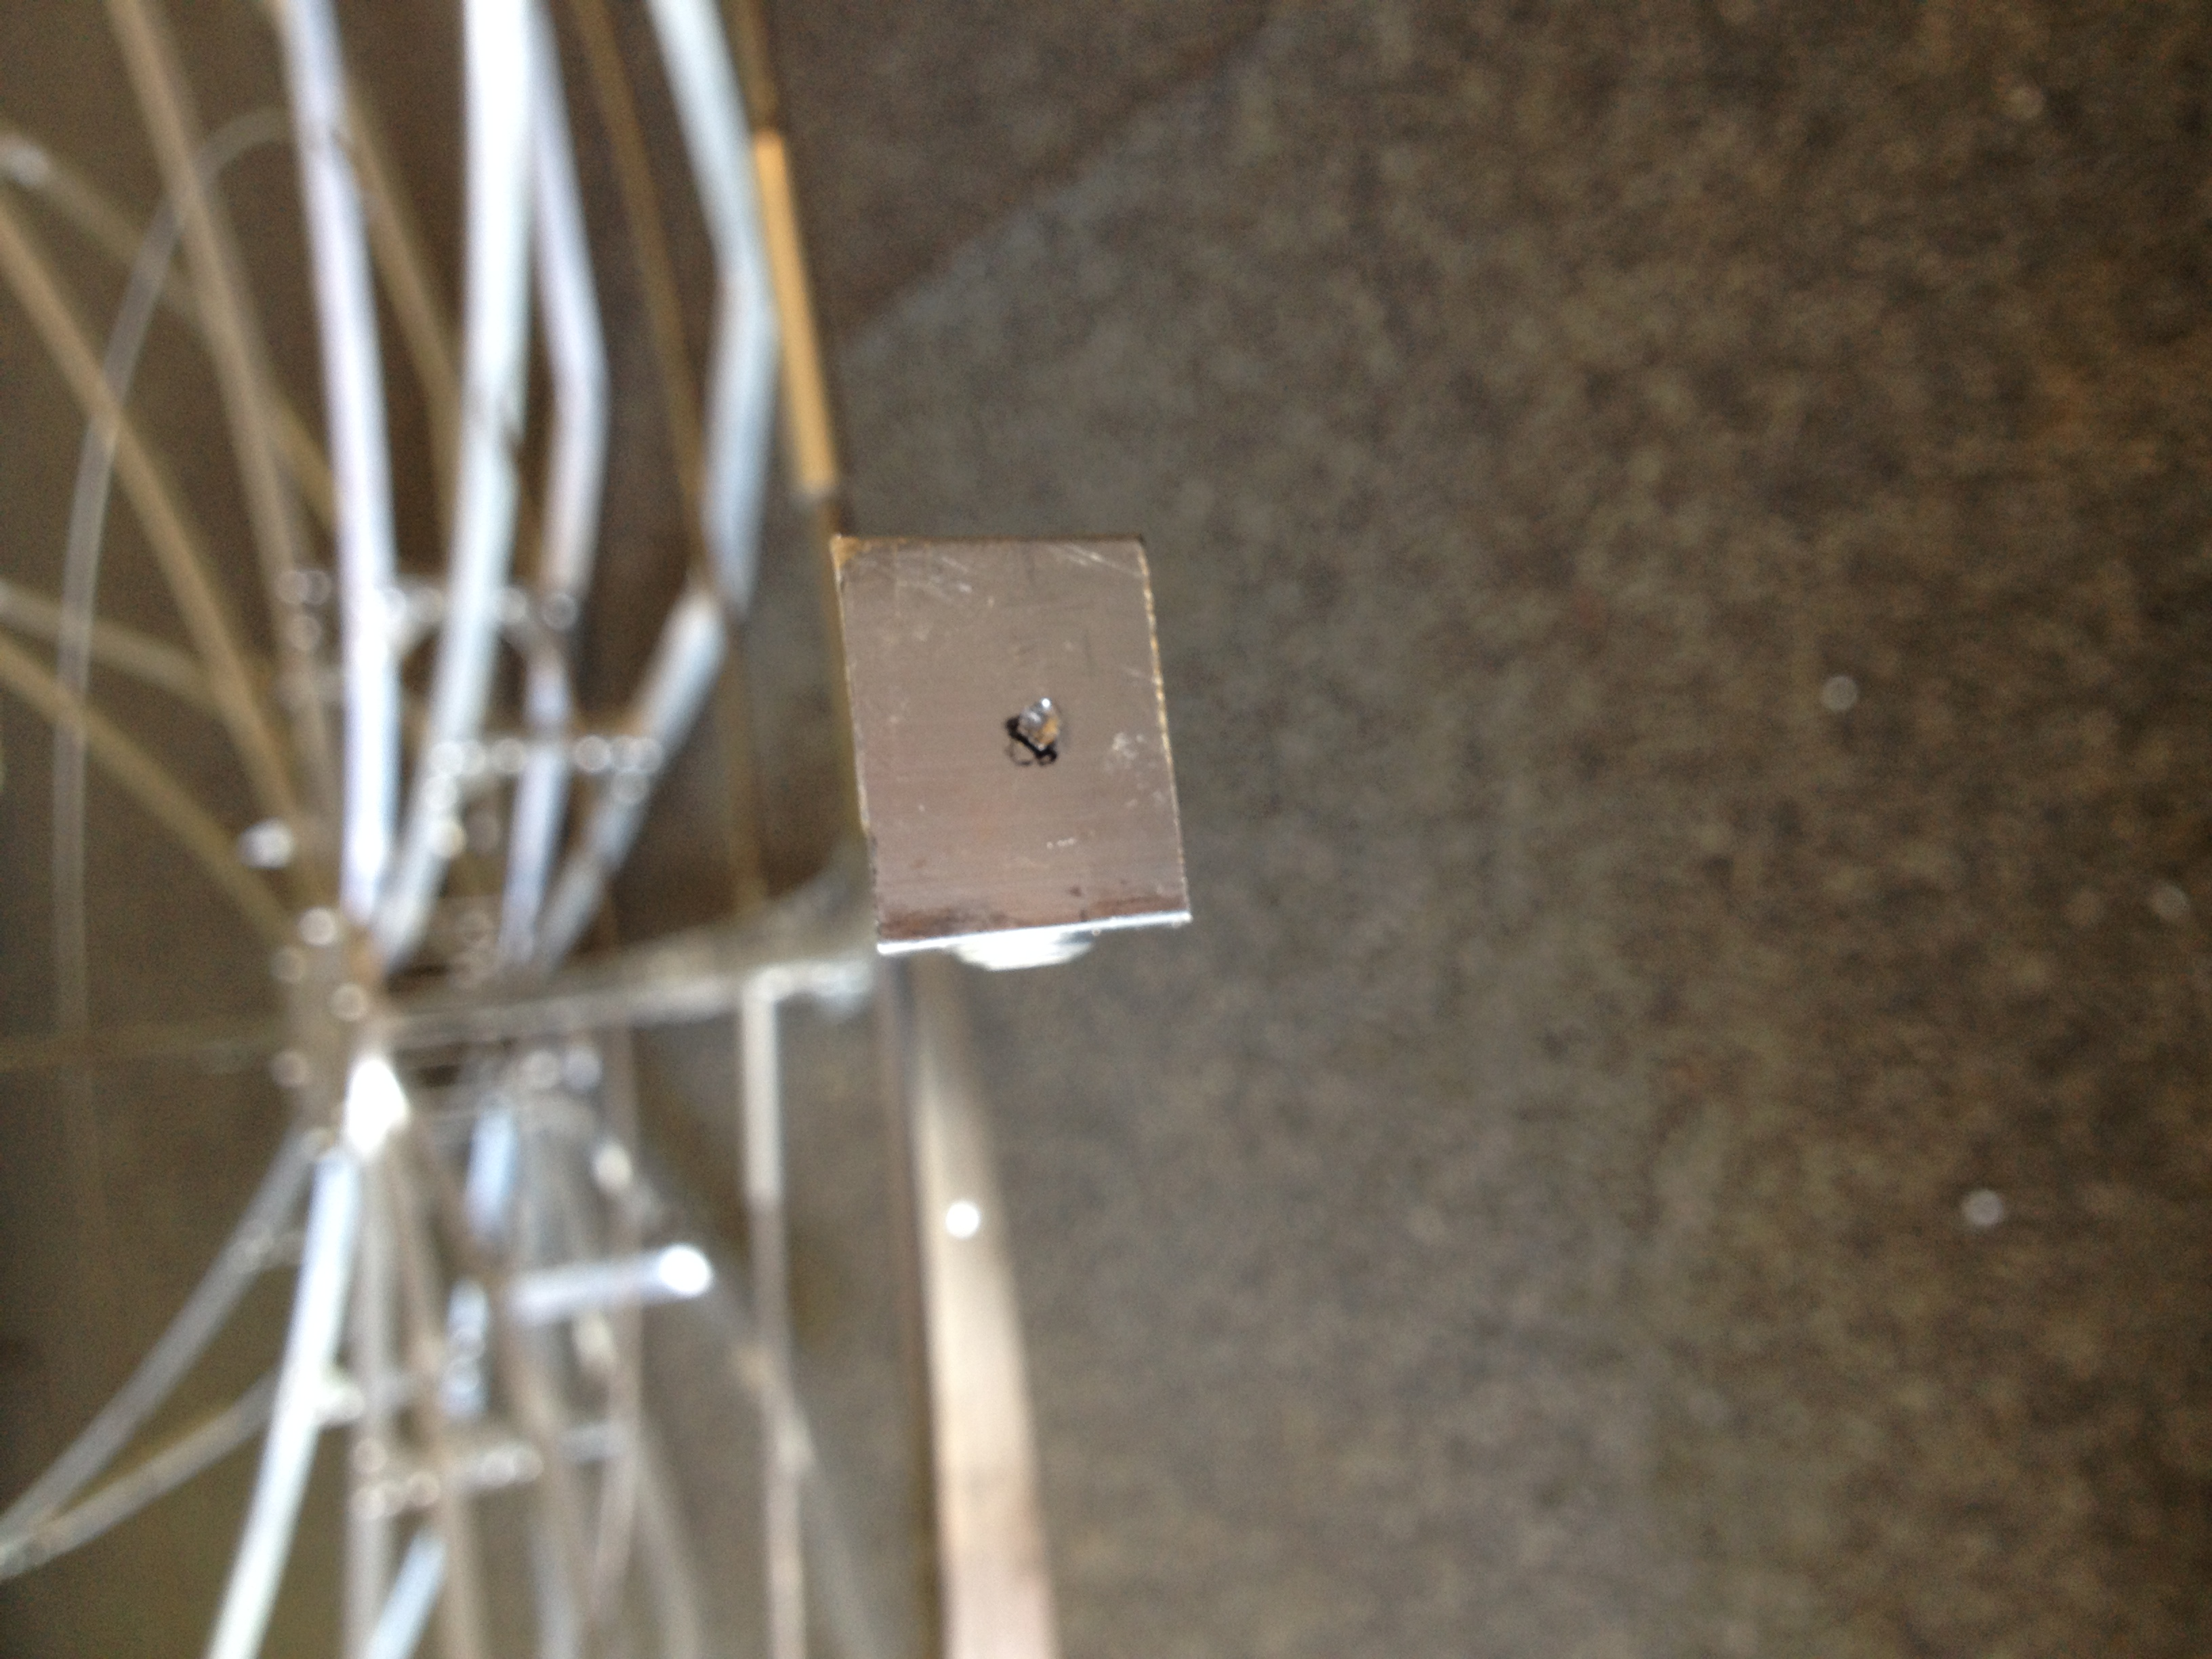
\includegraphics[scale=0.12]{dish/05.jpeg}
\end{center}

Then, using a power drill, holes were cut in both so they could be lined up and riveted.

\begin{center}
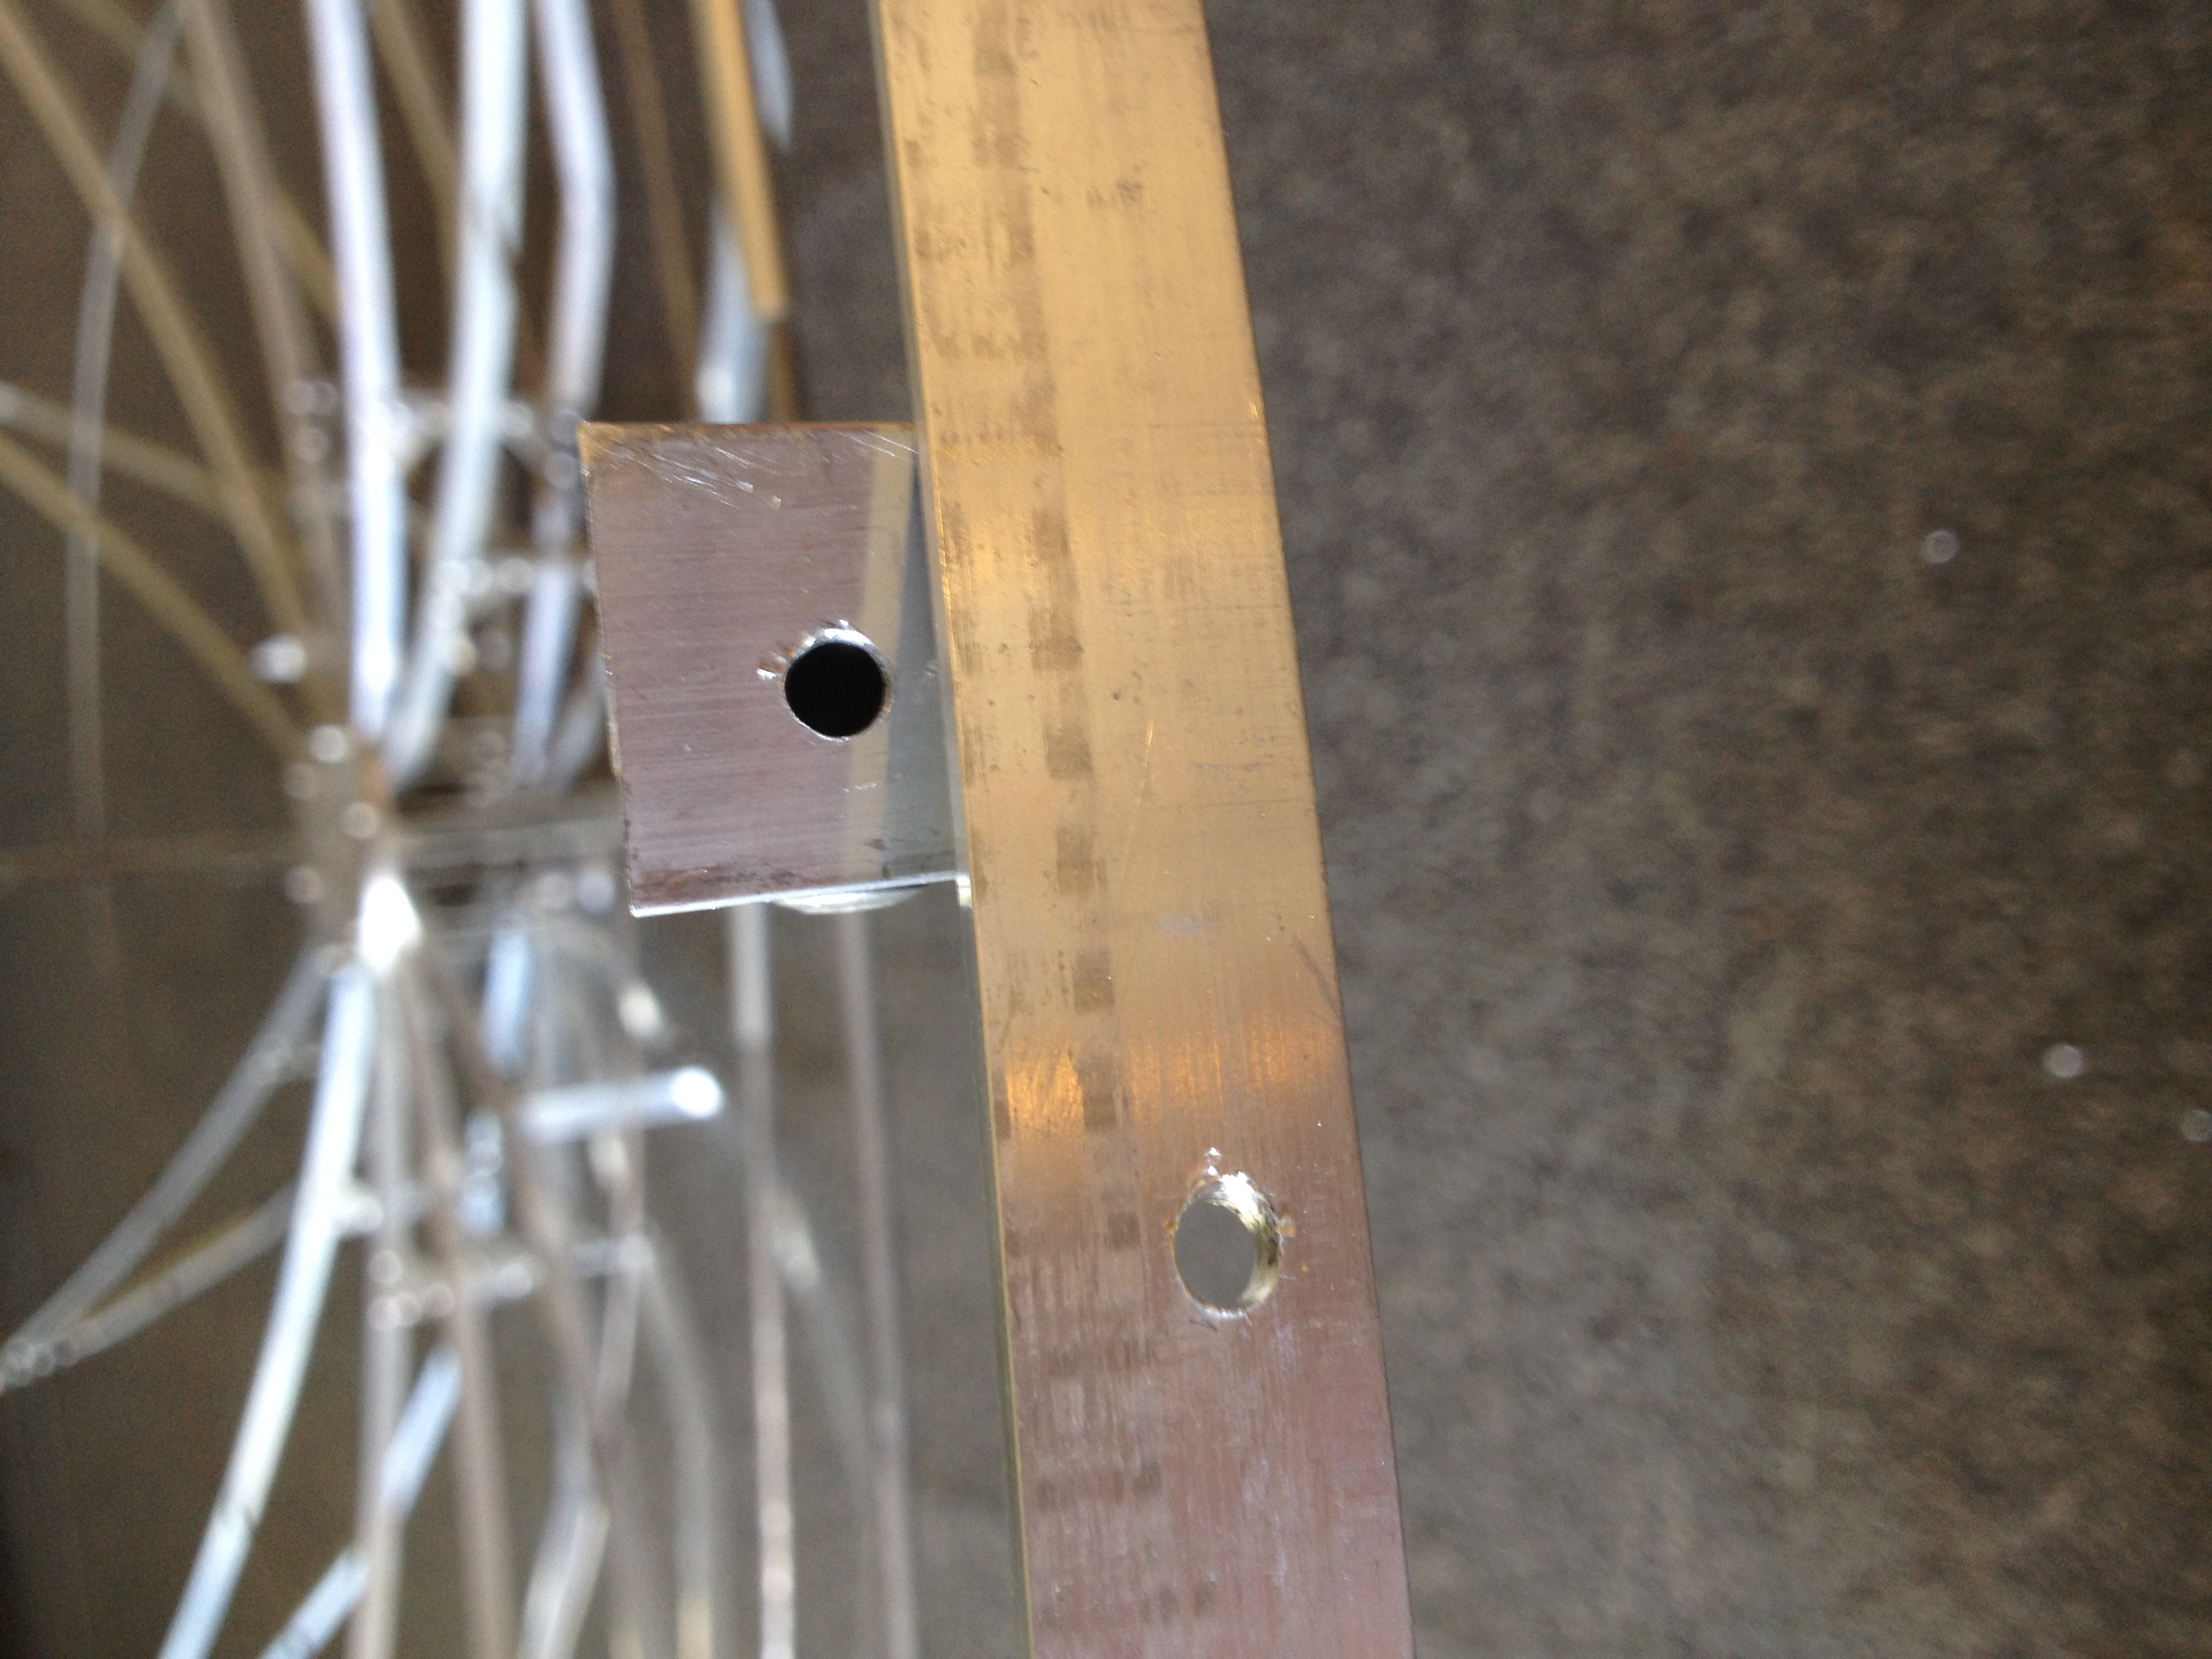
\includegraphics[scale=0.12]{dish/06.jpeg}
\end{center}


This process of tapping, drilling, and riveting was repeated for each of the 12 ribs of the dish. Once complete, we were ready to start putting the mesh on.

Make sure all the ends of the support rings are together. We did not crimp them, since they seemed secure enough so that they would not fall out.

\begin{center}
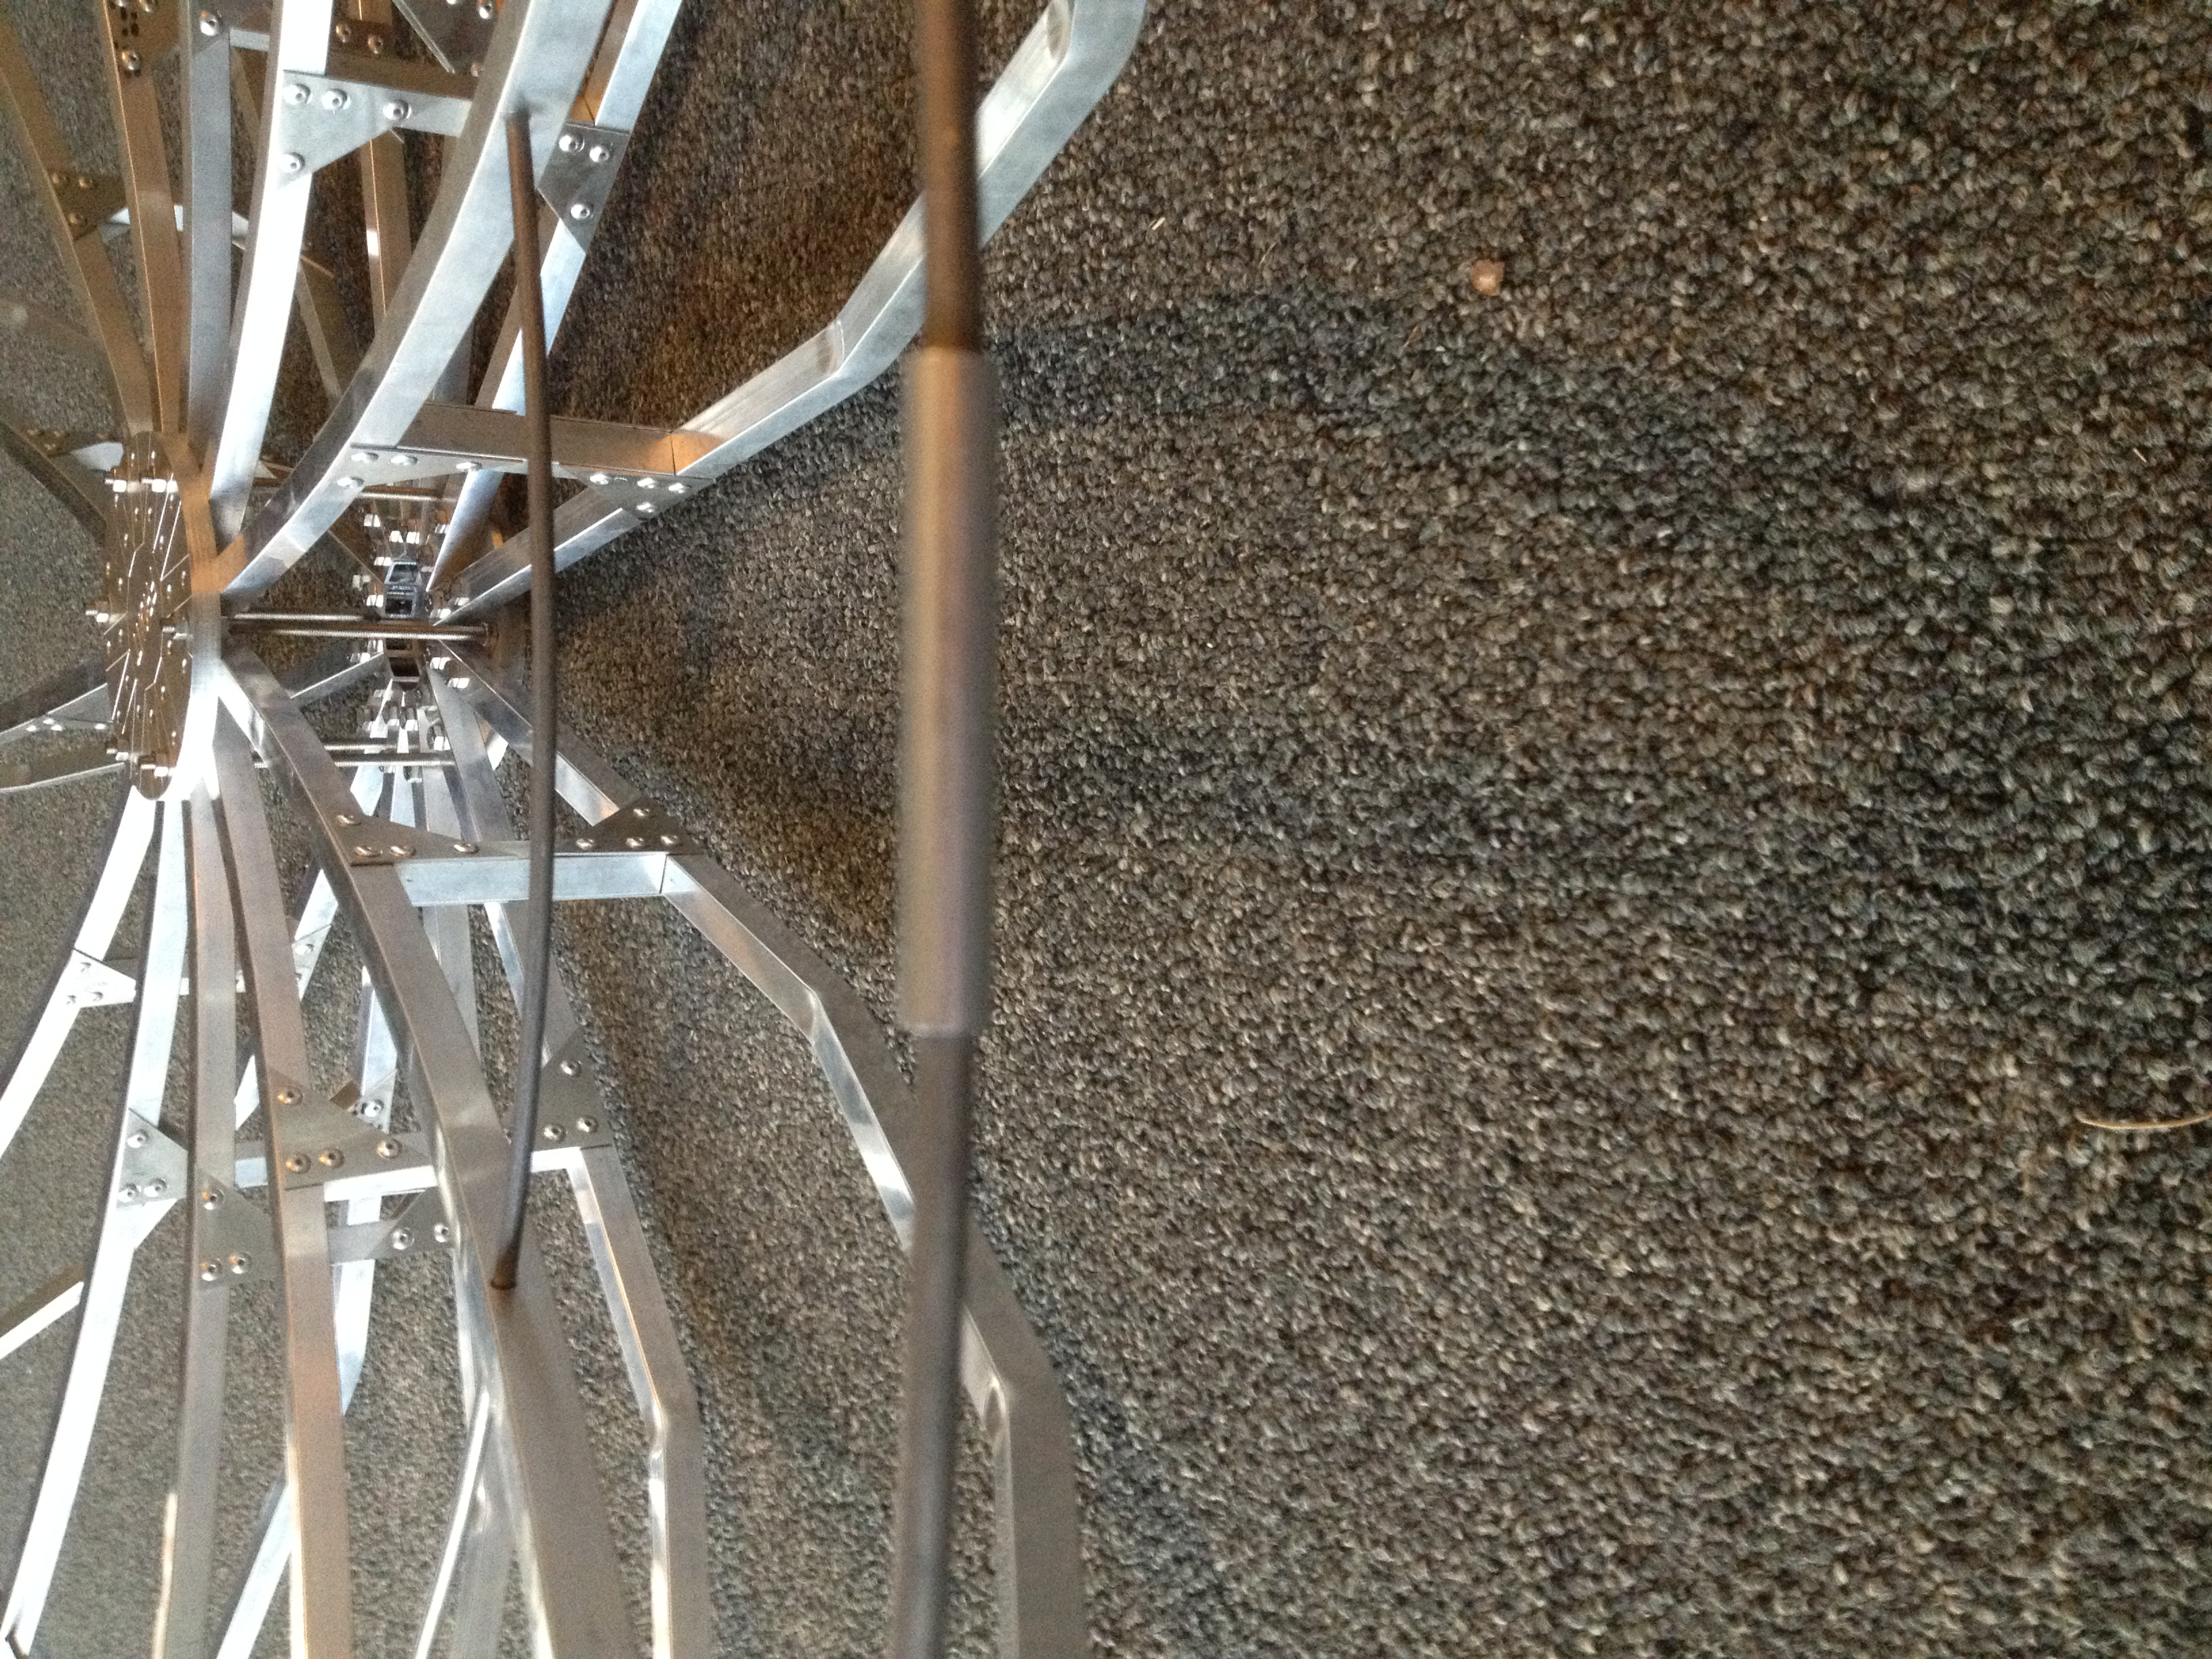
\includegraphics[scale=0.12]{dish/07.jpeg}
\end{center}

Cutting the mesh!

Below are some pictures that detail the mesh cutting process.



\begin{center}
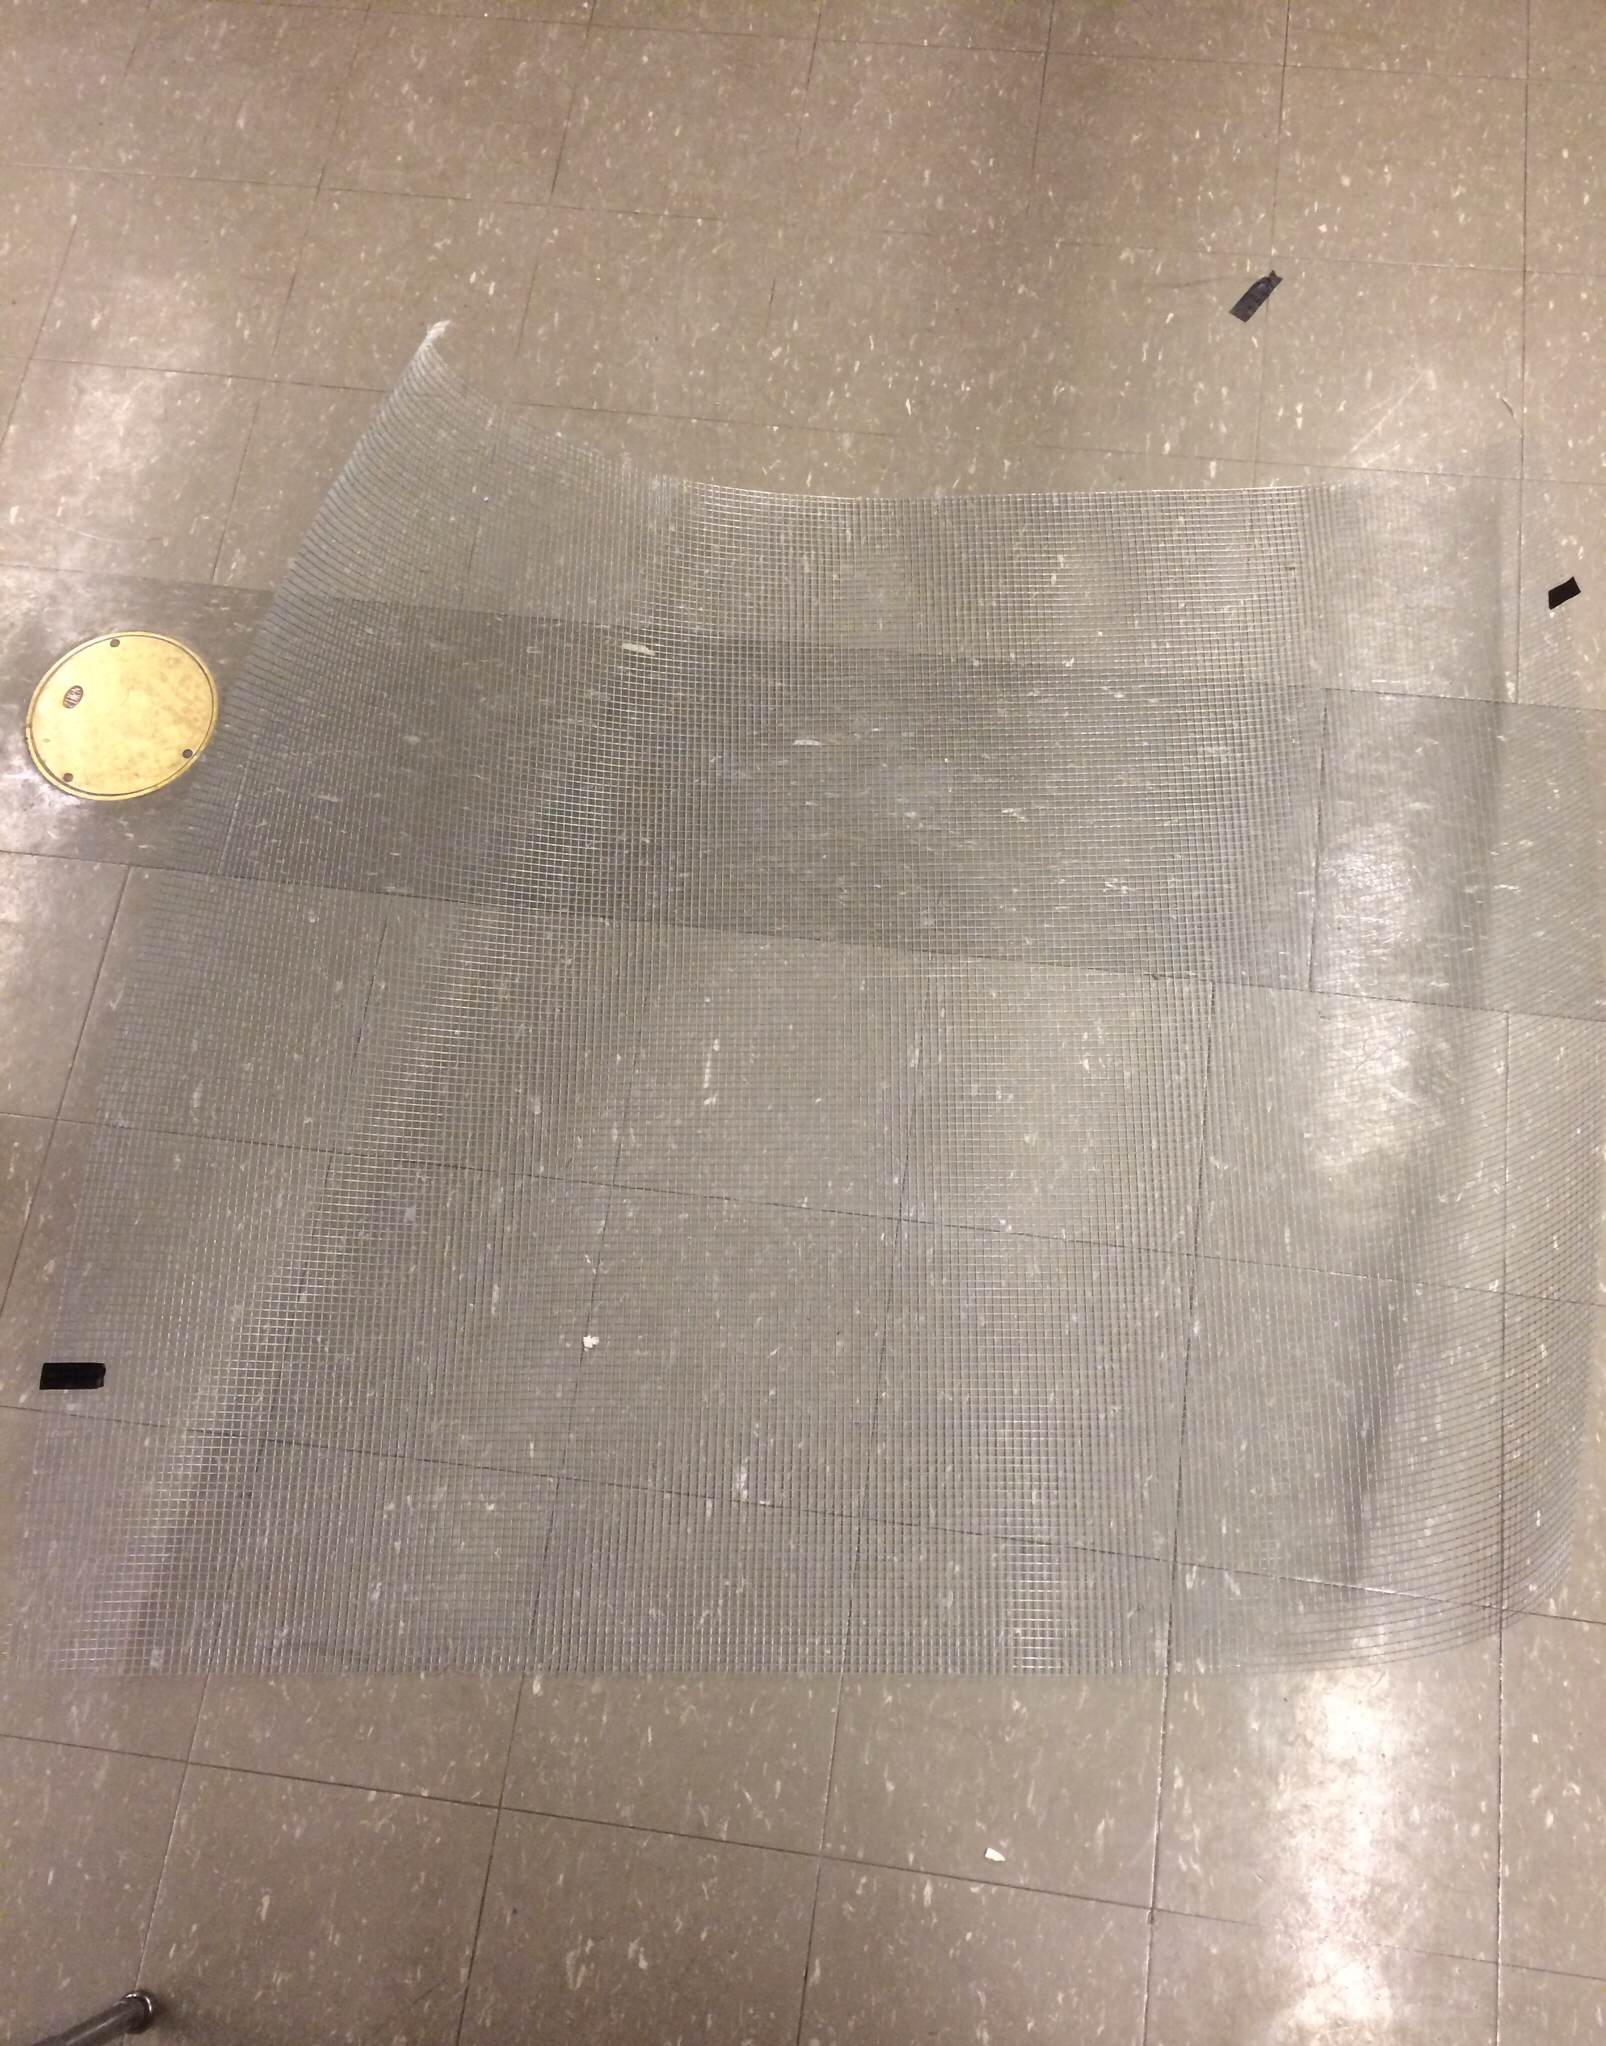
\includegraphics[scale=0.12]{dish/08.jpeg}
\end{center}

\begin{center}
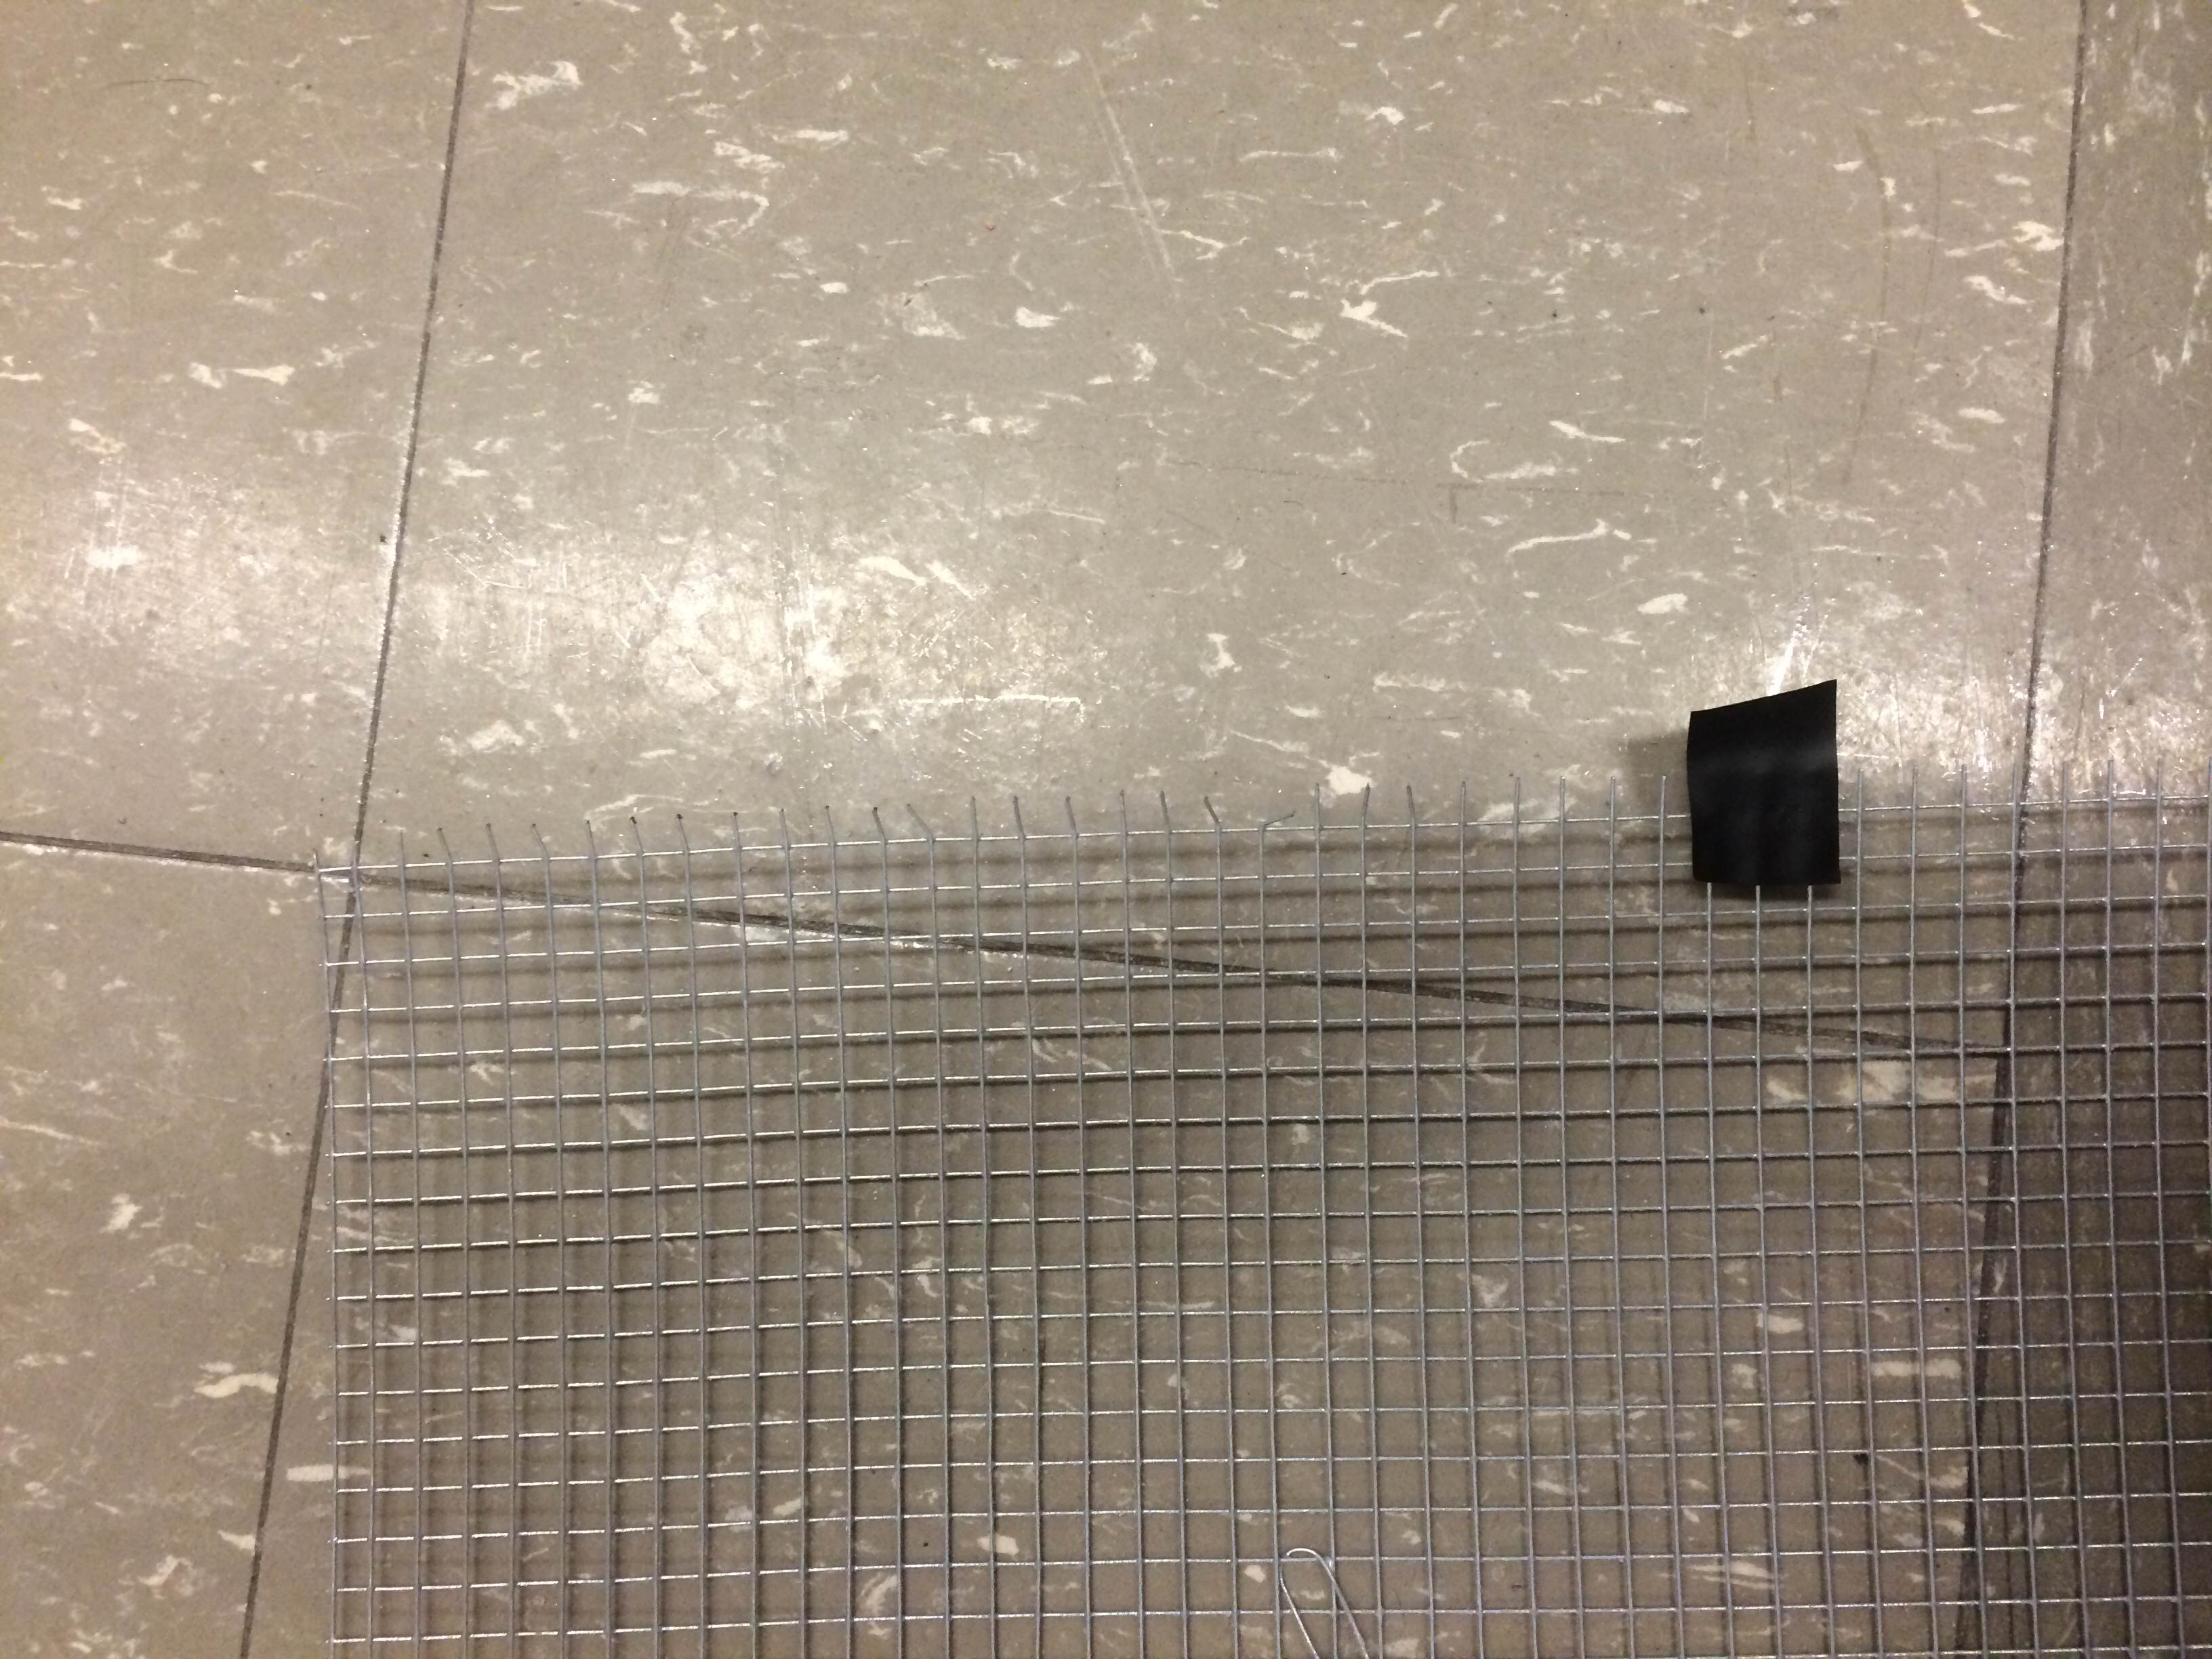
\includegraphics[scale=0.12]{dish/09.jpeg}
\end{center}

\begin{center}
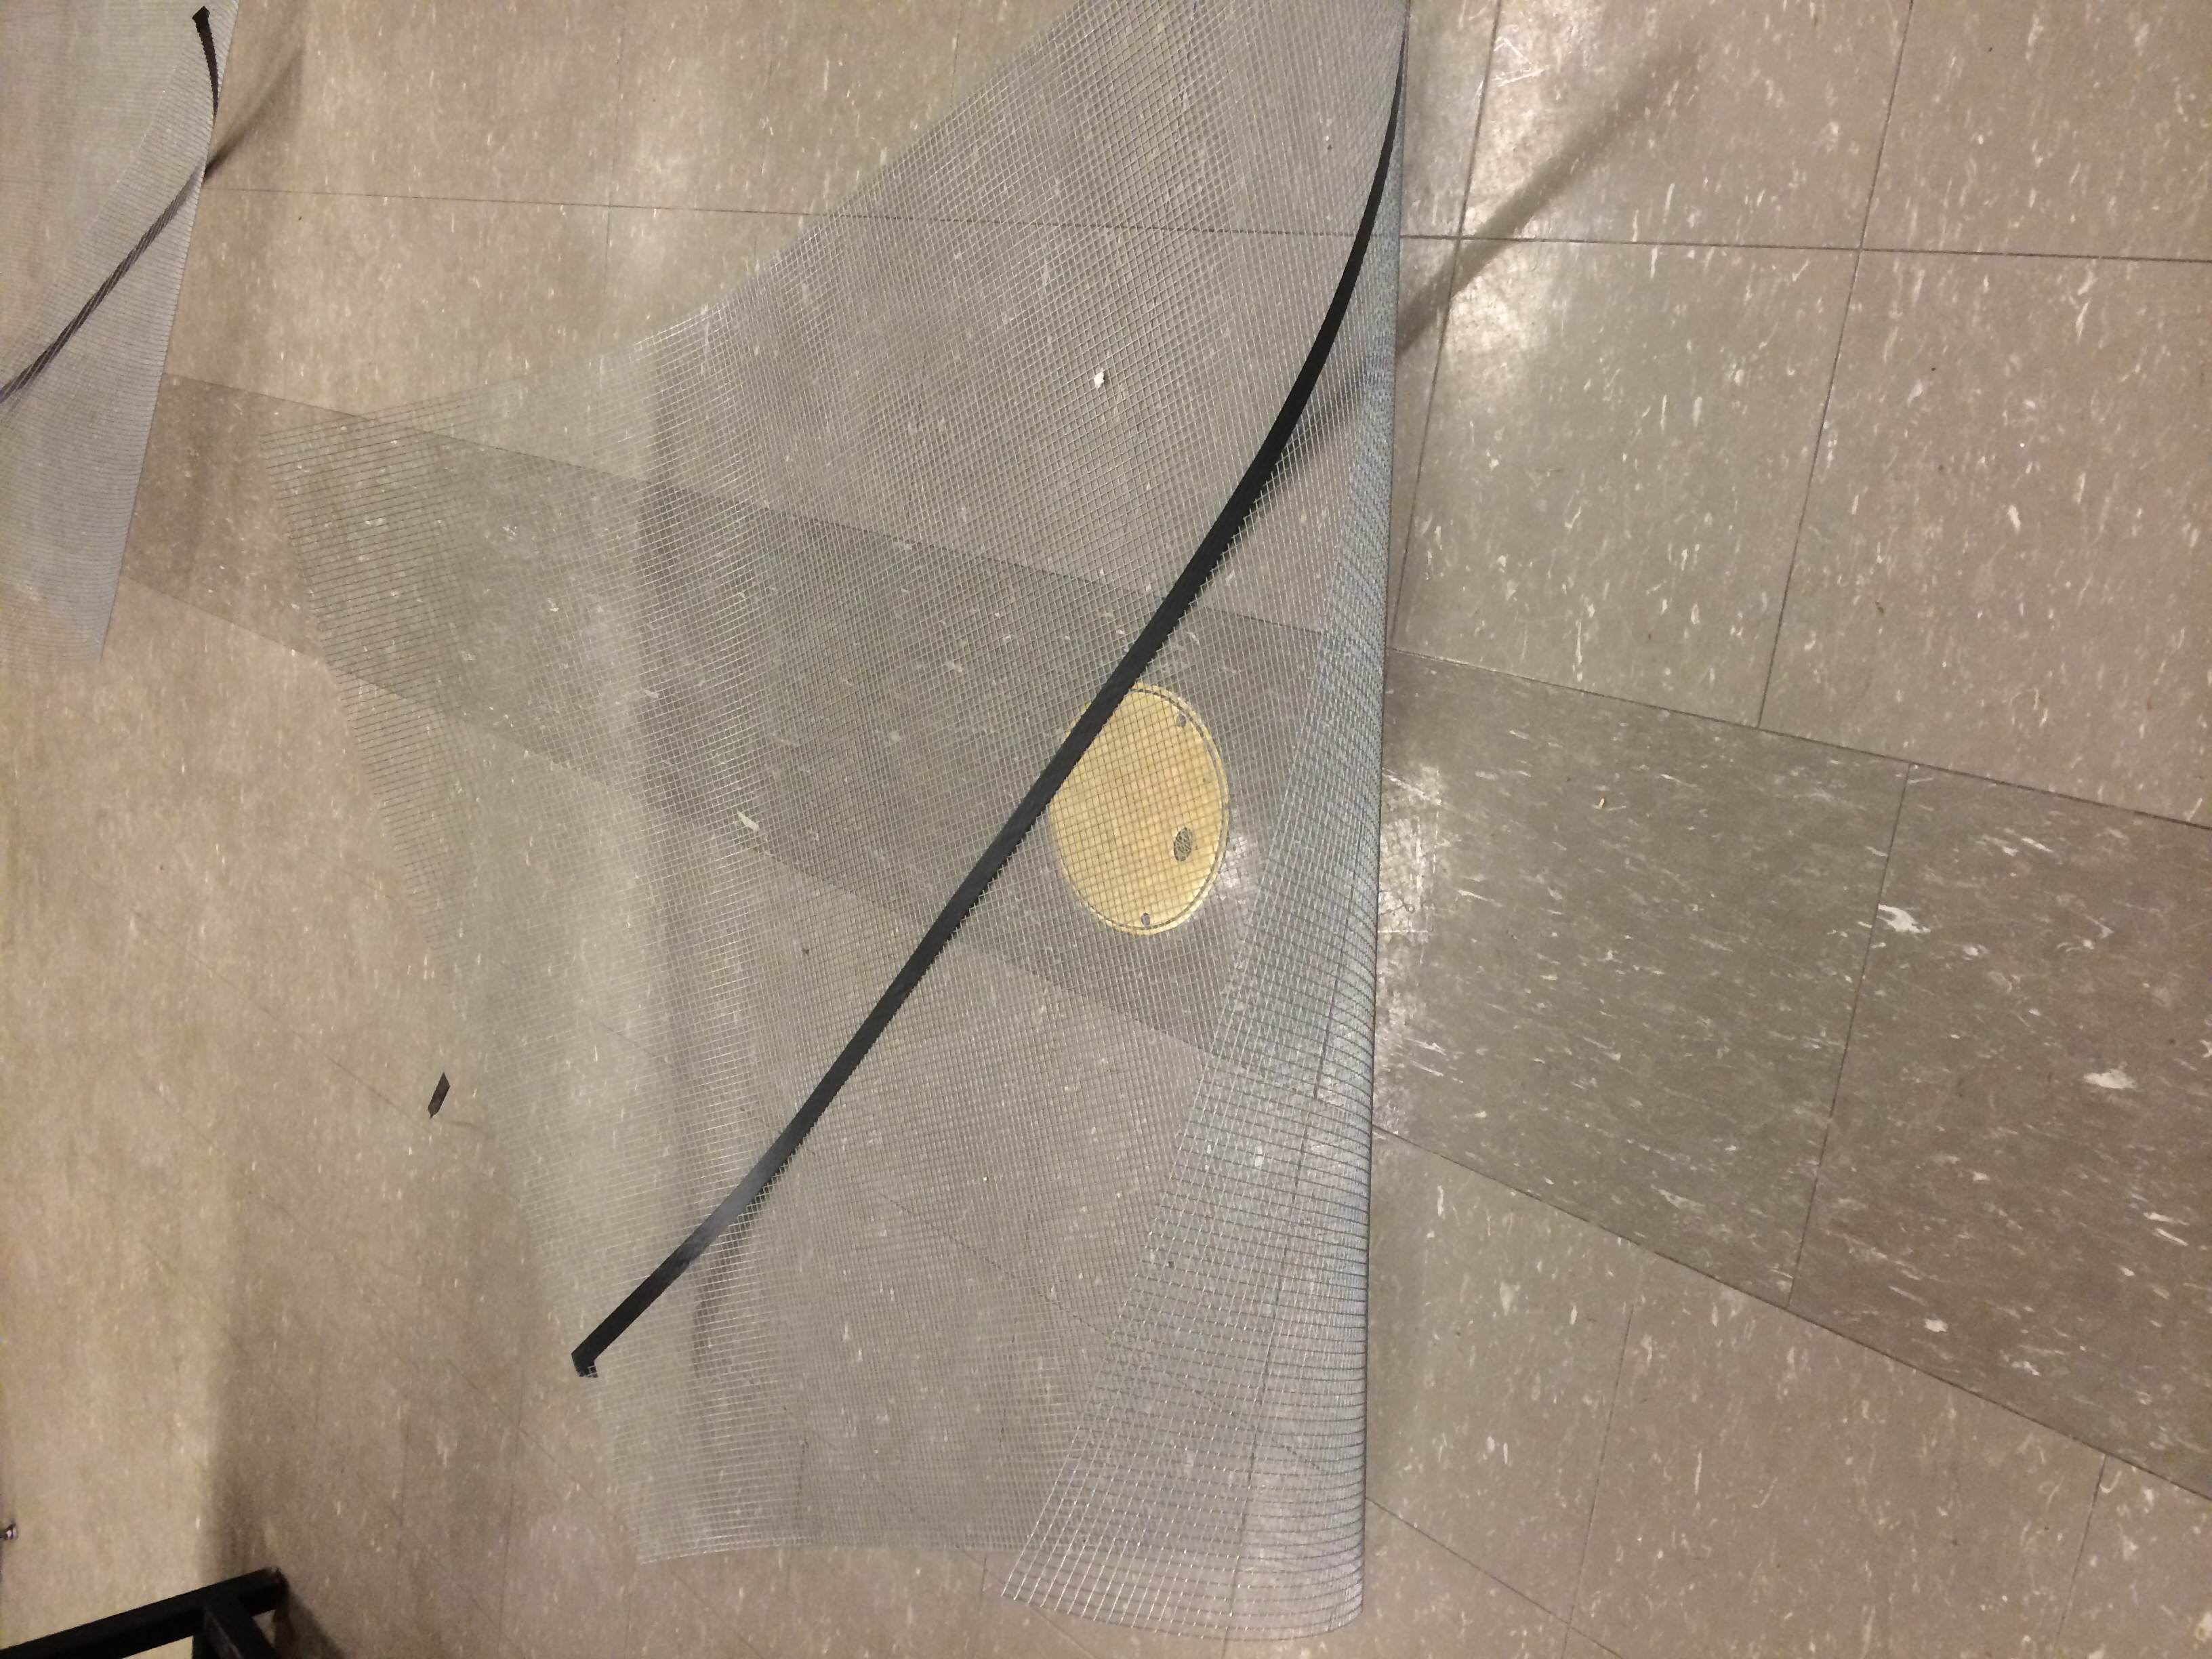
\includegraphics[scale=0.12]{dish/10.jpeg}
\end{center}

\begin{center}
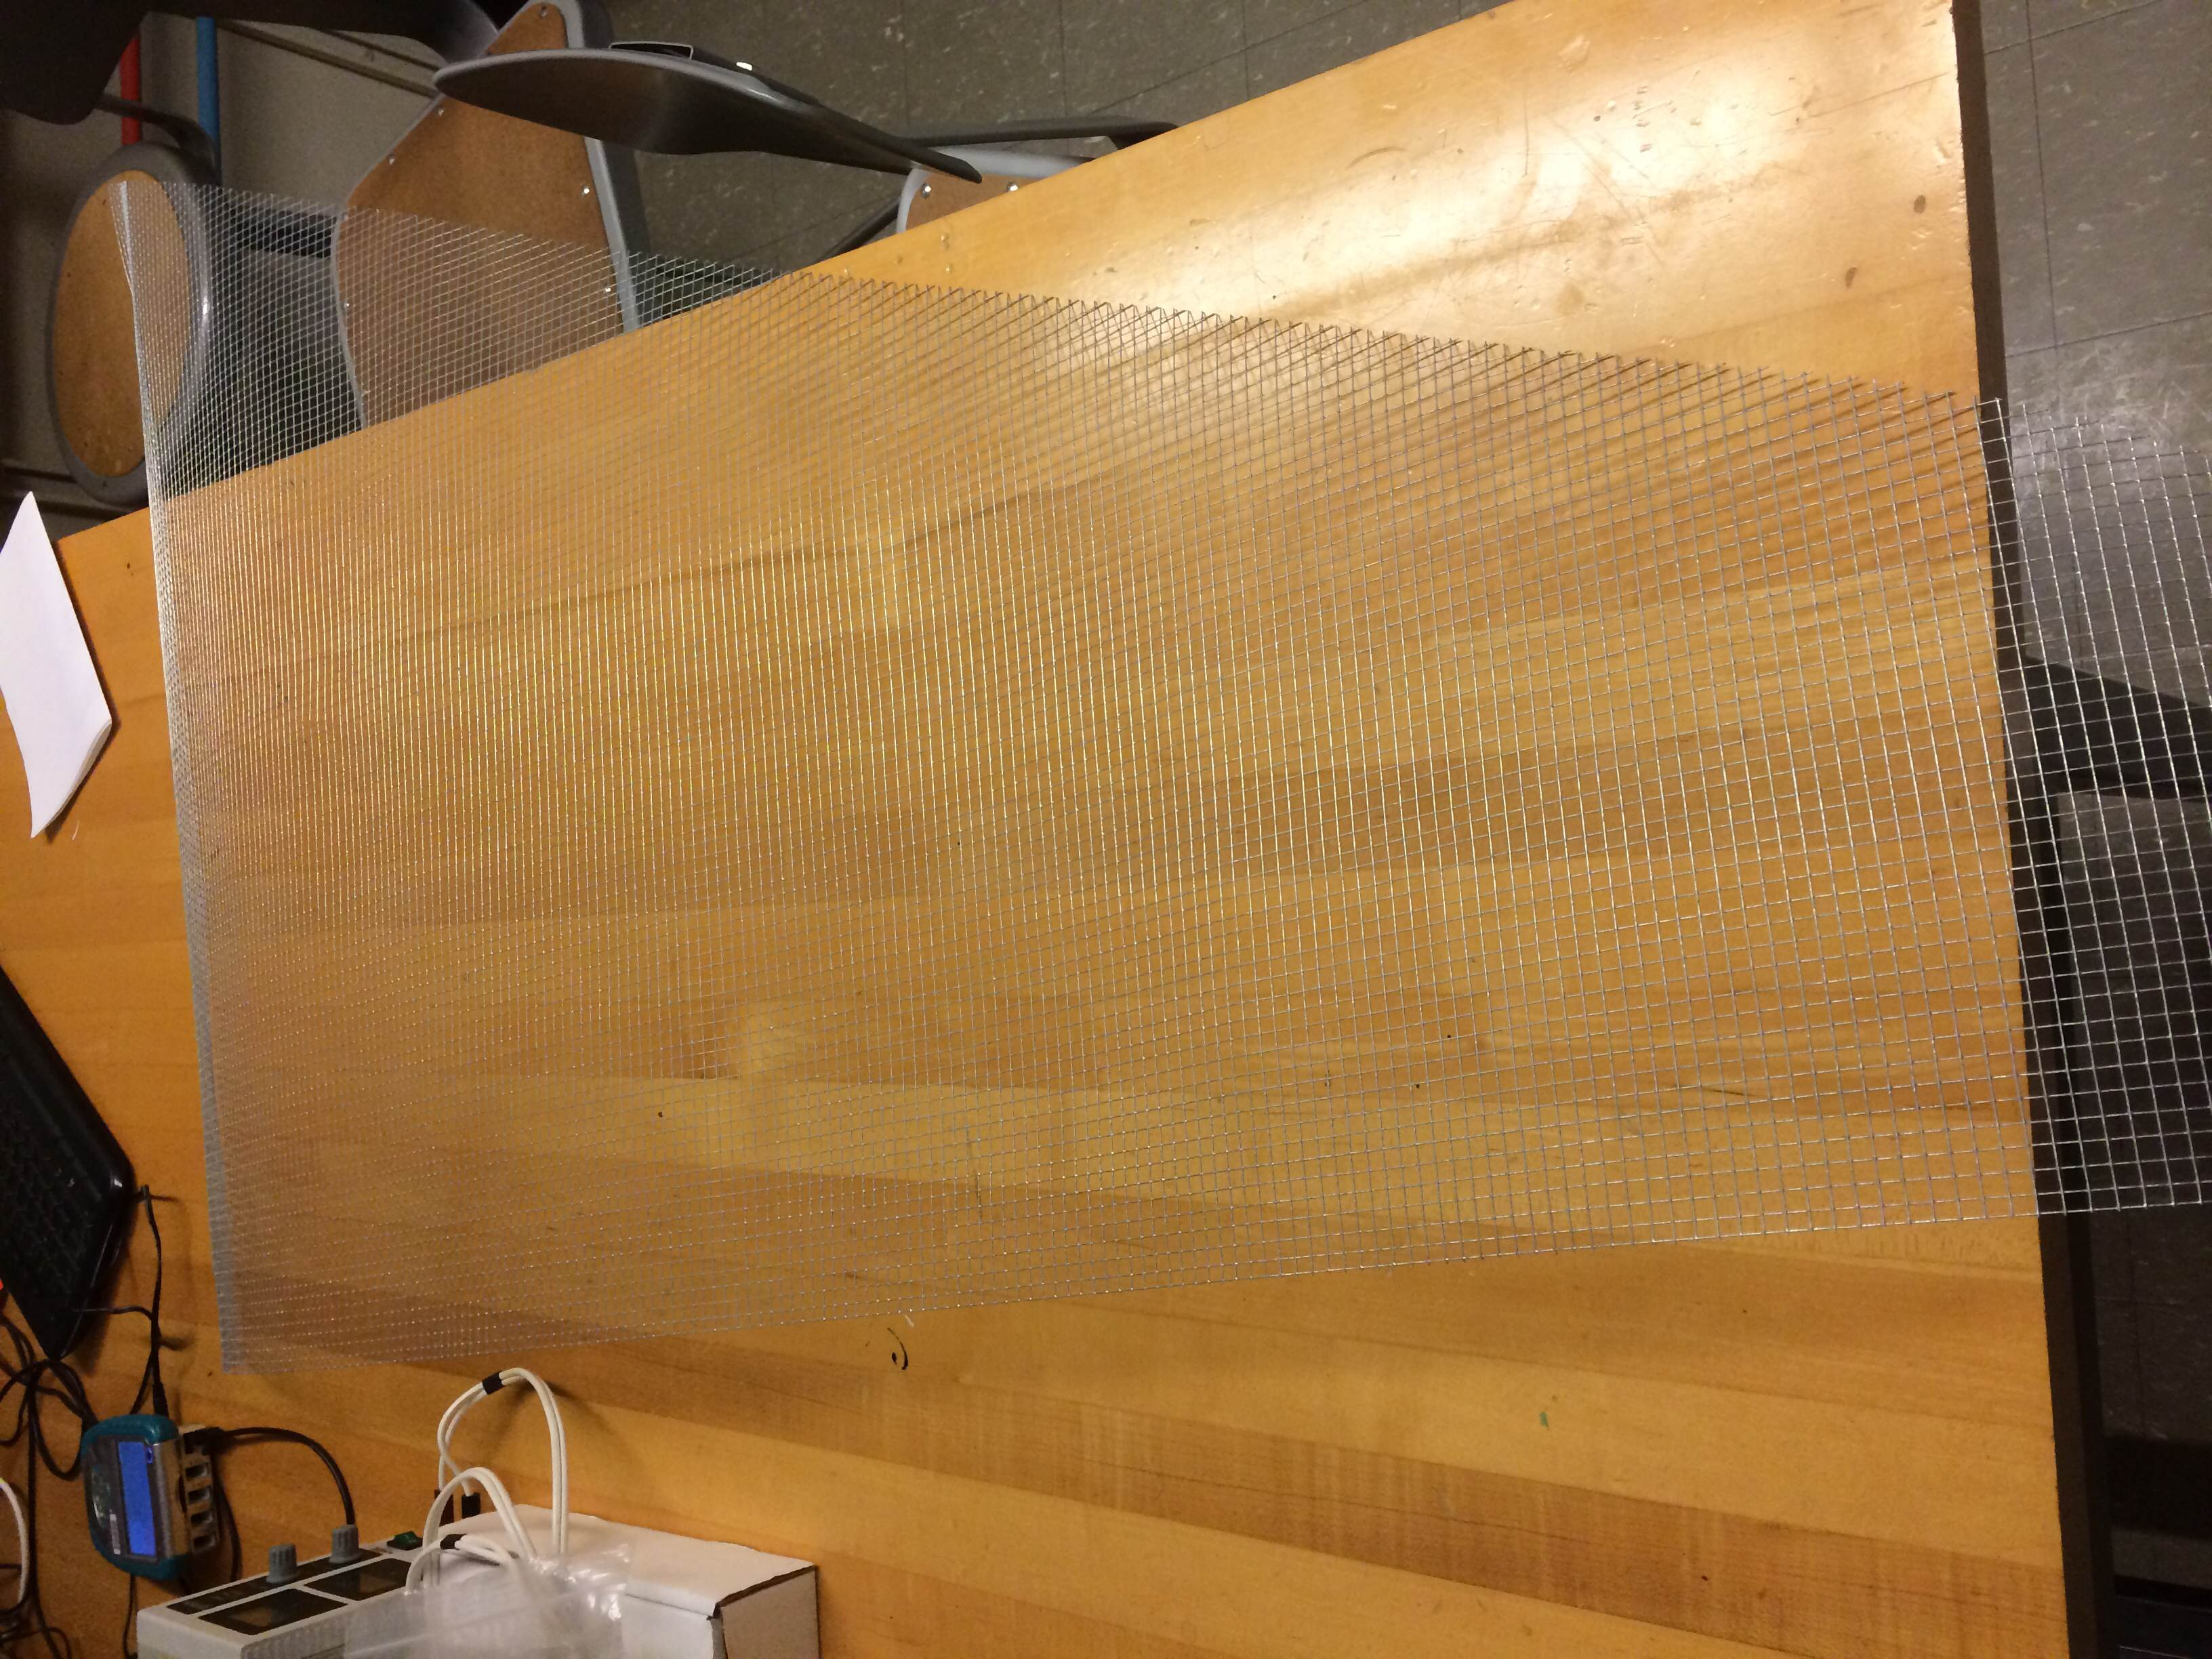
\includegraphics[scale=0.12]{dish/11.jpeg}
\end{center}


After the Mesh was cut to specifications, it was laid out on the skeleton of the dish, to make sure there was enough material and it would come together properly

\begin{center}
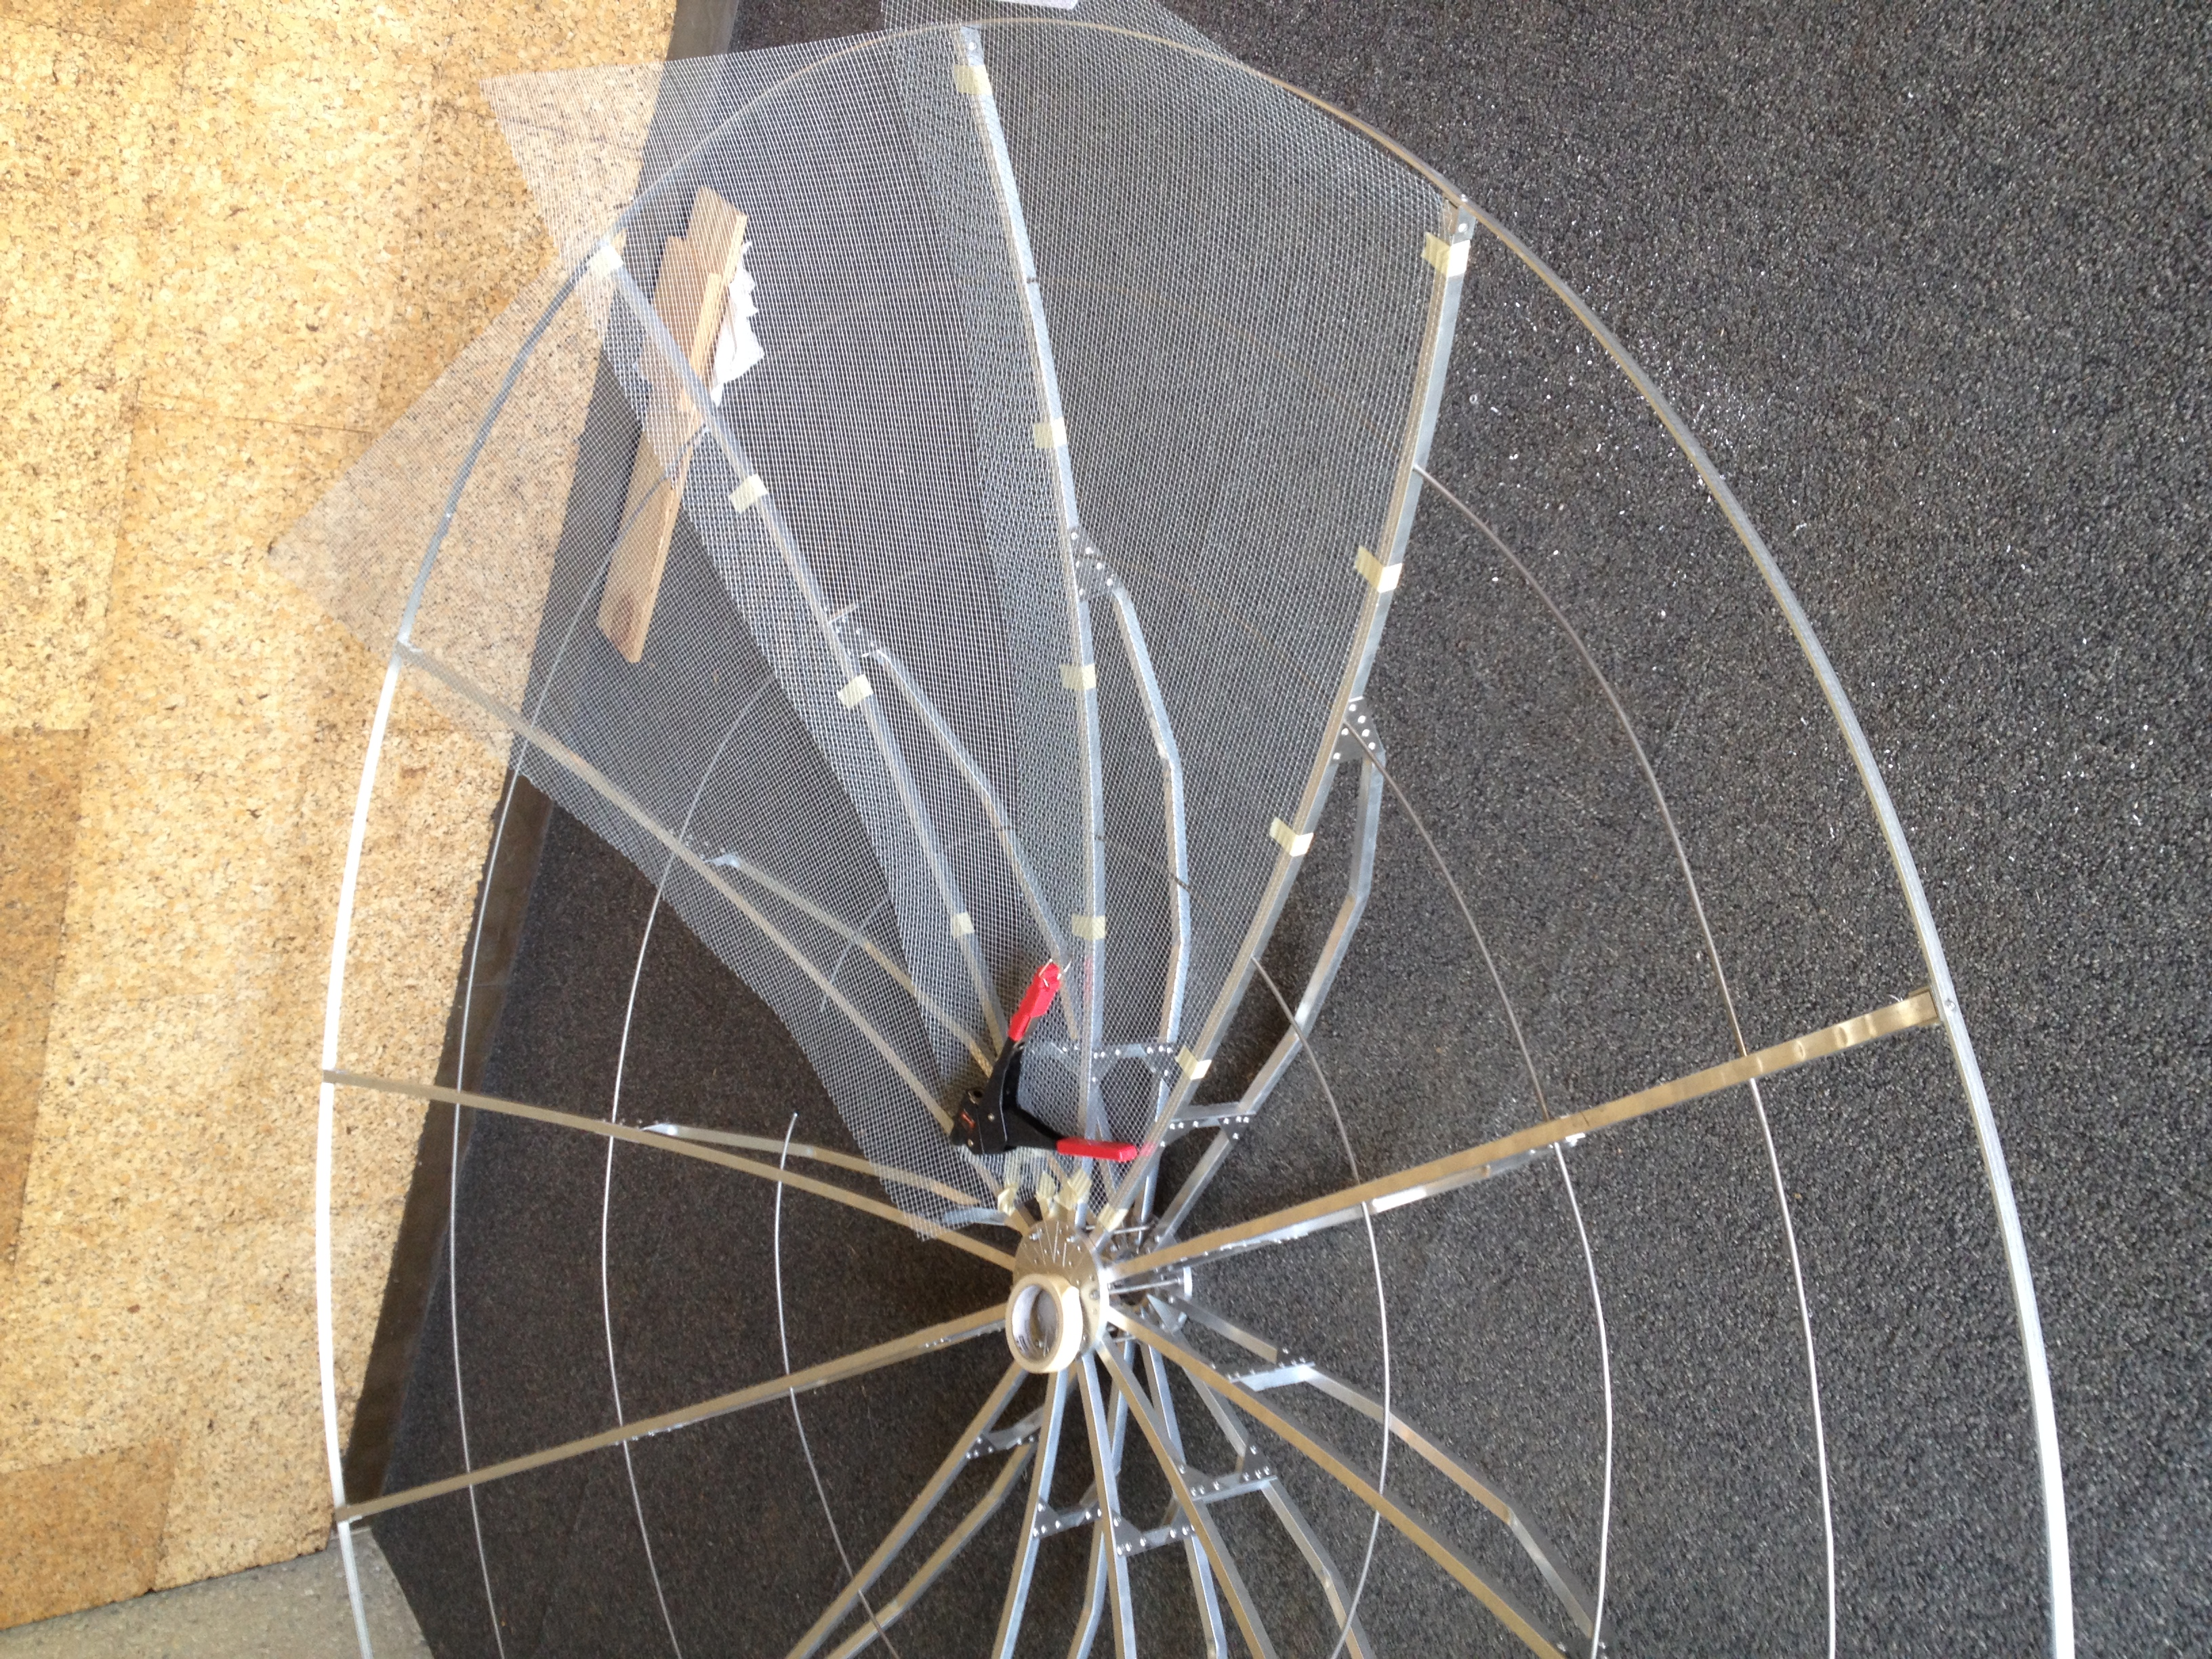
\includegraphics[scale=0.12]{dish/12.jpeg}
\end{center}

After we were sure that we had enough material all cut to the right size to allow for some extra, all the sheets were removed except for one. One end of the sheet was secured to a rib using tape, while the other end was trimmed down to be flush with the next rib

\begin{center}
\includegraphics[scale=0.12]{dish/13.jpeg}
\end{center}

Then, the next sheet is placed on top of the end of the first sheet so they are overlapping, and a strip with pre-drilled holes (which came with the kit) were lined up on top of the rib, and holes were drilled through the rib at the places where the holes in the strip were

\begin{center}
\includegraphics[scale=0.12]{dish/14.jpeg}
\end{center}

The strip, with the overlapping pieces of mesh underneath, was then riveted to the rib.

\begin{center}
\includegraphics[scale=0.12]{dish/15.jpeg}
\end{center}


This process was repeated for all 12 sections of the dish until it was complete.

\begin{center}
\includegraphics[scale=0.12]{dish/16.jpeg}
\end{center}

Then, the edges were trimmed, leaving about 1/4 to 1/2 inch mesh past the outer band (enough to wrap around the band a bit)

\begin{center}
\includegraphics[scale=0.12]{dish/17.jpeg}
\end{center}

It was then wrapped around the band

\begin{center}
\includegraphics[scale=0.12]{dish/18.jpeg}
\end{center}


And secured using zipties (~ 4 zipties per section * 12 sections = ~ 48 zipties)


\begin{center}
\includegraphics[scale=0.12]{dish/19.jpeg}
\end{center}

\end{document}
